\documentclass[british]{extarticle}

\usepackage[latin1]{inputenc}
\usepackage[T1]{fontenc}
%\usepackage{ae}
\usepackage[a4paper]{geometry}
\geometry{verbose,tmargin=3cm,bmargin=3cm,lmargin=3cm,rmargin=3cm,headheight=2cm,headsep=3cm,footskip=2cm}
\usepackage[light]{kpfonts}
\usepackage{amsmath, amssymb}
\usepackage{color}
\usepackage{graphicx,float}
\usepackage{parskip}
\usepackage{pstricks}
\usepackage{tikz}
\usepackage{scalefnt}
\usepackage{subfigure}
\usepackage{pdfpages}
\usepackage{wrapfig}
\usepackage[english]{babel}
\usepackage{tabularx}
%\usepackage[dvips,ps2pdf]{thumbpdf}
%\usepackage{textcomp}
\usepackage[font=small,labelfont=bf,textfont=it]{caption}
%\usepackage{caption2}
\usepackage{hyperref}

\numberwithin{figure}{section}
\let\footnote=\endnote
\hypersetup{colorlinks=true,linkcolor=black,citecolor=black}

%\hyphenpenalty=500

\includeonly{
	titlepage, 
	abstract,  
	toc, 
	%listofthings,
	section1-history_theory,
	section2-method, 
	section3-testing, 
	bib,
	appendix
}

\def\baselinestretch{1.3}

\begin{document}
\pagenumbering{roman}
%\begin{sloppypar}
\selectlanguage{english}

	\include{titlepage}
\setcounter{page}{1}
	\section*{Abstract}
\addcontentsline{toc}{section}{Abstract}
\thispagestyle{plain}

This report documents the building of the musical instrument known as the theremin, including the research, manufacture and subsequent testing of the product created. The instrument was made as an object intended to be understood rather than be economically or commercially viable in the form completed. Each stage was created so that it could be tested and added to the final assembly. Given more time, this could then be improved and developed into a finished product.

\vfill

\section*{Acknowledgements}
\addcontentsline{toc}{section}{Acknowledgements}
Many thanks to Tom Bryant for being a great lab partner, Dr.\ Signh and Mr.\ Barr for their help, advice and supervision, to the staff in the Physics and Astronomy stores for their patience and provision of components and Mark and Peter for their expertise and insights.

	\include{toc}

	\pagenumbering{arabic} 
\setcounter{page}{1}
\addcontentsline{toc}{part}{Building a Theremin}
\section{History and Theory}
\subsection{History}

The theremin was a product of research by the Russian government into proximity sensors and intelligence gathering. Lev Sergeivich Termen, known in Europe as Leon Theremin came across the apparatus' potential for sound production in October 1920. He showed it to Bolshevik leader Vladimir Lenin who dismissed the security value, but was incredibly impressed by the object as an instrument. He proposed that Theremin take it on a world tour to demonstrate the height of technology of the Soviet Union. This tour lasted until 1928 in Europe and, in 1929, he successfully patented the instrument in America. Despite the tour, the Theremin was not a commercial success until the mid 1930s and it fell into disuse after world war II when other electronic instruments came onto the market, such as the electric guitar, which had more immediate appeal though the sounds and relative easy of use. However, the theremin has remained a niche interest amongst electronic enthusiasts, such as Robert Moog, the inventor of the Moog Synthesiser and father of modern synthesizer technology.

The theremin was has had a variety of names, including the \ae therphone, thereminophone and termenvox and thereminvox. The final name was settled on after Theremin's death, using the Americanised version since that is where the patent was held at the time.

\subsection{Basic Theory}

The Theremin is an instrument which can be played without any physical contact from the user. This is certainly a contributing factor to its ongoing popularity amongst electronics enthusiasts such as Moog. 

The instrument uses two radio frequency oscillators to generate high frequency signals which are processed by a mixer. The mixer adds and subtracts the input signals and outputs a waveform which is chosen to be in the audible range, 20\,Hz to 20 000\,Hz. This method of converting high frequency signals down to lower frequency is known as heterodyning. One oscillator remains fixed whilst the other can be adjusted by a change in capacitance of the antenna connected to the instrument. The capacitor is formed by the user's hand, which is effectively a grounded plate, and the antenna. The resulting signal is amplified and played by a loud speaker.

This method of sound production allows for a wide, continuous range of frequencies, over the whole human audible range, and for different types of sound to be produced through the addition of post production effects being added to the waveform before being played. It also gives the instrument a unique sound that is sometimes desired in situations such as TV soundtracks.

\subsubsection{Generation - Oscillators}

The oscillators used come under the class of VCOs, voltage control oscillators, as the input voltage is directly proportional to the frequency of the signal generated. 

\begin{wrapfigure}[10]{r}{0.4\textwidth}
  \begin{center}
    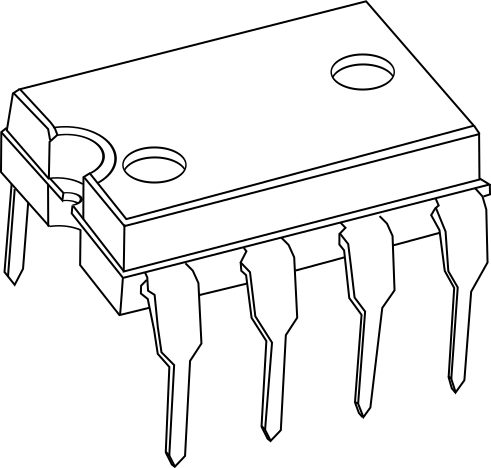
\includegraphics[width=0.3\textwidth]{report_img/ic}
  \end{center}
  \caption{A 555 timer integrated circuit VCO for use in bread board electronics.}
  \label{fig:timer ic}
\end{wrapfigure}

The VCOs are given an input voltage and output a series of pulses with a high time and low time determined by their governing equations. These equations are calculated by the manufacturers and vary between models, specific cases are discussed in sections~\ref{sec:555},~\ref{sec:4046} and~\ref{sec:7555}. This high-low nature means that the output signal is a close approximation to a square wave. A perfect sound wave is sinusoidal so this is not the ideal case, however, later stages in signal processing lead to the shape changing slightly and the difference in audible quality due to the wave not being sinusoidal is slight.

The VCOs are complete components supplied in the form of an monolithic integrated circuit, called an IC. They comprise a variety of components that shall be treated as a complete separate entity. These ICs are included in the circuit to perform a particular action, the inner workings will not be considered for this report.

\subsubsection{Control - Capacitor}
The capacitor is a simple parallel plate capacitor, one plate formed by the antenna, connected to the circuit, the other being the user's hand, or any other body part or other conducting object, that is near the first plate. The user is effectively grounded so the capacitor is connected once to the circuit and once to ground, as shown in figure~\ref{fig:capacitor}. The capacitor equation is given by,

\begin{figure}[htbp]
  \begin{center}
    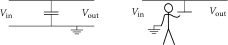
\includegraphics[scale=1.2]{report_img/plate_capacitor}
    \caption{A capacitor is used to control the sound produced by the circuit. When in the theremin, the capacitor is replaced by an antenna and a separate plate formed of the user's hand.}
    \label{fig:capacitor}
  \end{center}
\end{figure}

When the user moves closer to the plate, the capacitance decreases and, likewise, the capacitance increases when the user moves away. Also the area of plate, i.e.\ the size of the user's hand, will change the capacitance, in accordance with the capacitor equation, equation~(\ref{eqn:capacitor}), which gives another mode of control over the sound produced.
\begin{align}
  C &= \frac{k\varepsilon_0 A}{d}, \label{eqn:capacitor}
\end{align}
where,
\begin{itemize}
  \item $k$ is the relative permittivity of the dielectric material between the plates, in this case air which has $k=1$,
  \item $\varepsilon_0$ is the permittivity of free space, $\varepsilon_0 = 8.85 \times 10^{-12} \text{Fm}^{-1}$,
  \item $A$ is the area of the plates and
  \item $d$ is the separation of the two plates.
\end{itemize}

\newpage 

	\section{Method}
\subsection{Oscillator - 555 Timer IC}
\label{sec:555}
The first attempt made for the oscillators is to use a 555 timer chip to directly create an audible frequency square wave signal. The frequency of the 555 IC is determined by the size of the resistances, $R_1$ and $R_2$, and the capacitor, $C$, as located in figure~\ref{fig:555}.

\begin{figure}[htbp]
	\begin{center}
		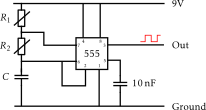
\includegraphics[scale=1.2]{report_img/555}
		\caption{Circuit diagram of the 555 timer IC with the immediate components used to make a VCO.}
		\label{fig:555}
	\end{center}
\end{figure}

The signal is generated by the chip using a series of capacitors and components contained within, a circuit diagram for the 555 can be seen in appendix~\ref{app:555}. The chip is connected in the astable mode so that the output signal is a continuous stream of rectangular pulses with a given frequency that obey equations (\ref{eqn:555freq}), (\ref{eqn:555high}) and (\ref{eqn:555low}), where $\tau_{\text{high}}$ is the time spent in the high voltage position and $\tau_{\text{low}}$ is the low time.\cite{NE555}
\begin{align}
	\label{eqn:555freq}
	f &= \frac{1}{\ln{2}C(R_1+R_2)}, \\
	\label{eqn:555high}
	\tau_{\text{high}} &= \ln{2}C(R_1+R_2), \\
	\label{eqn:555low}
	\tau_{\text{low}} &= \ln{2}CR_2. 
\end{align}
With two chips combined, a high degree of control over the output can be achieved by varying the value of the resistors. As a proof of concept, the circuit in figure \ref{fig:2x555} was built and a variable resistor in the form of an LDR was added. This allowed the pitch and volume to be controlled remotely using the fingers.

\begin{figure}[htbp]
	\begin{center}
		
\includegraphics[scale=0.8,angle=90]{report_img/2x555}
		\caption{Circuit diagram of the two 555 timer ICs used to make a rudimentary resistance controlled theremin.}
		\label{fig:2x555}
	\end{center}
\end{figure}

\subsection{Oscillator - HEF4046 IC}
\label{sec:4046}
Though a controllable waveform in the audible frequency range was produced using the previously described 555 timer method, the sound was not pleasant as the wave was square shape and so does not resemble the ideal sinusoidal sound wave. In an attempt to improve the quality of this sound, an alternative VCO chip is tried. The first choice is the 8068 chip but this is no longer in commercial production, so a close relative, the 4046 chip, is used.

This chip contains several components that shall not be used, but importantly has a voltage controlled oscillator that can be used independently. The circuit diagram is shown in appendix~\ref{app:4046}. Pins 4, 6, 7, 10, 13, 15 and 16 are used with others left open.

Under these conditions, with a capacitance of 10\,nF and resistance of 10\,k$\Omega$, an audible sound was produced, shown, as measured on an oscilloscope, in figure~\ref{fig:4046square}.

\begin{figure}[htbp]
	\centering
		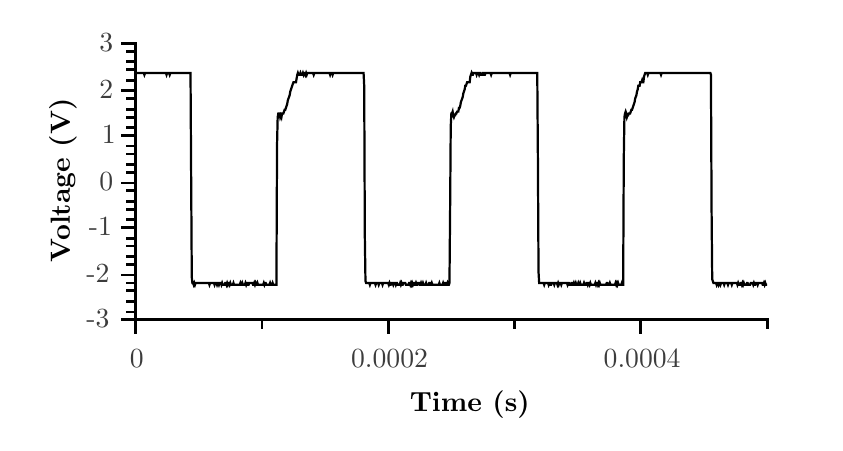
\begin{tikzpicture}{0pt}{0pt}{299pt}{150pt}
	\clip(0pt,150pt) -- (284.325pt,150pt) -- (284.325pt,7.36184pt) -- (0pt,7.36184pt) -- (0pt,150pt);
\begin{scope}
	\clip(38.9878pt,144.294pt) -- (267.209pt,144.294pt) -- (267.209pt,44.4478pt) -- (38.9878pt,44.4478pt) -- (38.9878pt,144.294pt);
	\color[gray]{0}
	\draw[line width=0.8pt, line join=miter, line cap=rect](39.216pt,133.644pt) -- (39.4442pt,133.644pt) -- (39.6724pt,133.644pt) -- (39.9006pt,133.644pt) -- (40.1289pt,133.644pt) -- (40.3571pt,133.644pt) -- (40.5853pt,133.644pt) -- (40.8135pt,133.644pt) -- (41.0418pt,133.644pt) -- (41.27pt,133.644pt) -- (41.4982pt,133.644pt) -- (41.7264pt,133.644pt) -- (41.9546pt,133.644pt) -- (42.1829pt,132.979pt) -- (42.4111pt,133.644pt) -- (42.6393pt,133.644pt) -- (42.8675pt,133.644pt) -- (43.0957pt,133.644pt) -- (43.324pt,133.644pt) -- (43.5522pt,133.644pt) -- (43.7804pt,133.644pt) -- (44.0086pt,133.644pt) -- (44.2368pt,133.644pt) -- (44.4651pt,133.644pt) -- (44.6933pt,133.644pt) -- (44.9215pt,133.644pt) -- (45.1497pt,133.644pt) -- (45.378pt,133.644pt) -- (45.6062pt,133.644pt) -- (45.8344pt,133.644pt) -- (46.0626pt,133.644pt) -- (46.2908pt,133.644pt) -- (46.5191pt,133.644pt) -- (46.7473pt,133.644pt) -- (46.9755pt,133.644pt) -- (47.2037pt,133.644pt) -- (47.4319pt,133.644pt) -- (47.6602pt,133.644pt) -- (47.8884pt,133.644pt) -- (48.1166pt,133.644pt) -- (48.3448pt,133.644pt) -- (48.573pt,133.644pt) -- (48.8013pt,133.644pt) -- (49.0295pt,133.644pt) -- (49.2577pt,133.644pt) -- (49.4859pt,133.644pt) -- (49.7142pt,133.644pt) -- (49.9424pt,133.644pt) -- (50.1706pt,132.979pt) -- (50.3988pt,133.644pt) -- (50.627pt,133.644pt) -- (50.8553pt,133.644pt) -- (51.0835pt,133.644pt) -- (51.3117pt,132.979pt) -- (51.5399pt,133.644pt) -- (51.7681pt,133.644pt) -- (51.9964pt,133.644pt) -- (52.2246pt,133.644pt) -- (52.4528pt,133.644pt) -- (52.681pt,133.644pt) -- (52.9092pt,133.644pt) -- (53.1375pt,133.644pt) -- (53.3657pt,133.644pt) -- (53.5939pt,133.644pt) -- (53.8221pt,133.644pt) -- (54.0504pt,133.644pt) -- (54.2786pt,133.644pt) -- (54.5068pt,133.644pt) -- (54.735pt,133.644pt) -- (54.9632pt,133.644pt) -- (55.1915pt,133.644pt) -- (55.4197pt,133.644pt) -- (55.6479pt,133.644pt) -- (55.8761pt,133.644pt) -- (56.1043pt,133.644pt) -- (56.3326pt,133.644pt) -- (56.5608pt,133.644pt) -- (56.789pt,133.644pt) -- (57.0172pt,133.644pt) -- (57.2454pt,133.644pt) -- (57.4737pt,133.644pt) -- (57.7019pt,133.644pt) -- (57.9301pt,133.644pt) -- (58.1583pt,133.644pt) -- (58.3866pt,133.644pt) -- (58.6148pt,133.644pt) -- (58.843pt,133.644pt) -- (59.0712pt,95.7024pt) -- (59.2994pt,59.7576pt) -- (59.5277pt,57.7607pt) -- (59.7559pt,57.7607pt) -- (59.9841pt,57.095pt) -- (60.2123pt,57.7607pt) -- (60.4405pt,57.095pt) -- (60.6688pt,57.7607pt) -- (60.897pt,57.7607pt) -- (61.1252pt,57.7607pt) -- (61.3534pt,57.7607pt) -- (61.5816pt,57.7607pt) -- (61.8099pt,57.7607pt) -- (62.0381pt,57.7607pt) -- (62.2663pt,57.7607pt) -- (62.4945pt,57.7607pt) -- (62.7228pt,57.7607pt) -- (62.951pt,57.7607pt) -- (63.1792pt,57.7607pt) -- (63.4074pt,57.7607pt) -- (63.6356pt,57.7607pt) -- (63.8639pt,57.7607pt) -- (64.0921pt,57.7607pt) -- (64.3203pt,57.7607pt) -- (64.5485pt,57.7607pt) -- (64.7767pt,57.7607pt) -- (65.005pt,57.7607pt) -- (65.2332pt,57.7607pt) -- (65.4614pt,57.7607pt) -- (65.6896pt,57.095pt) -- (65.9178pt,57.7607pt) -- (66.1461pt,57.7607pt) -- (66.3743pt,57.7607pt) -- (66.6025pt,57.7607pt) -- (66.8307pt,57.7607pt) -- (67.059pt,57.7607pt) -- (67.2872pt,57.7607pt) -- (67.5154pt,57.095pt) -- (67.7436pt,57.7607pt) -- (67.9718pt,57.7607pt) -- (68.2001pt,57.7607pt) -- (68.4283pt,57.095pt) -- (68.6565pt,57.7607pt) -- (68.8847pt,57.7607pt) -- (69.1129pt,57.095pt) -- (69.3412pt,57.7607pt) -- (69.5694pt,57.7607pt) -- (69.7976pt,57.7607pt) -- (70.0258pt,57.095pt) -- (70.254pt,57.7607pt) -- (70.4823pt,57.095pt) -- (70.7105pt,57.095pt) -- (70.9387pt,57.095pt) -- (71.1669pt,57.095pt) -- (71.3952pt,57.7607pt) -- (71.6234pt,57.7607pt) -- (71.8516pt,57.095pt) -- (72.0798pt,57.7607pt) -- (72.308pt,57.095pt) -- (72.5363pt,57.7607pt) -- (72.7645pt,57.7607pt) -- (72.9927pt,57.095pt) -- (73.2209pt,57.7607pt) -- (73.4491pt,57.095pt) -- (73.6774pt,57.095pt) -- (73.9056pt,57.095pt) -- (74.1338pt,57.095pt) -- (74.362pt,57.7607pt) -- (74.5902pt,57.095pt) -- (74.8185pt,57.095pt) -- (75.0467pt,57.095pt) -- (75.2749pt,57.095pt) -- (75.5031pt,57.095pt) -- (75.7314pt,57.095pt) -- (75.9596pt,57.095pt) -- (76.1878pt,57.095pt) -- (76.416pt,57.095pt) -- (76.6442pt,57.095pt) -- (76.8725pt,57.7607pt) -- (77.1007pt,57.095pt) -- (77.3289pt,57.095pt) -- (77.5571pt,57.7607pt) -- (77.7853pt,57.095pt) -- (78.0136pt,57.095pt) -- (78.2418pt,57.095pt) -- (78.47pt,57.095pt) -- (78.6982pt,57.7607pt) -- (78.9264pt,57.095pt) -- (79.1547pt,57.7607pt) -- (79.3829pt,57.7607pt) -- (79.6111pt,57.095pt) -- (79.8393pt,57.095pt) -- (80.0676pt,57.7607pt) -- (80.2958pt,57.7607pt) -- (80.524pt,57.7607pt) -- (80.7522pt,57.7607pt) -- (80.9804pt,57.7607pt) -- (81.2087pt,57.7607pt) -- (81.4369pt,57.095pt) -- (81.6651pt,57.095pt) -- (81.8933pt,57.7607pt) -- (82.1215pt,57.095pt) -- (82.3498pt,57.7607pt) -- (82.578pt,57.095pt) -- (82.8062pt,57.095pt) -- (83.0344pt,57.7607pt) -- (83.2626pt,57.095pt) -- (83.4909pt,57.095pt) -- (83.7191pt,57.095pt) -- (83.9473pt,57.095pt) -- (84.1755pt,57.095pt) -- (84.4038pt,57.095pt) -- (84.632pt,57.095pt) -- (84.8602pt,57.095pt) -- (85.0884pt,57.095pt) -- (85.3166pt,57.7607pt) -- (85.5449pt,57.095pt) -- (85.7731pt,57.7607pt) -- (86.0013pt,57.7607pt) -- (86.2295pt,57.095pt) -- (86.4577pt,57.095pt) -- (86.686pt,57.095pt) -- (86.9142pt,57.095pt) -- (87.1424pt,57.095pt) -- (87.3706pt,57.095pt) -- (87.5988pt,57.7607pt) -- (87.8271pt,57.095pt) -- (88.0553pt,57.095pt) -- (88.2835pt,57.095pt) -- (88.5117pt,57.7607pt) -- (88.74pt,57.095pt) -- (88.9682pt,57.095pt) -- (89.1964pt,57.095pt) -- (89.4246pt,57.095pt) -- (89.6528pt,57.095pt) -- (89.8811pt,57.095pt) -- (90.1093pt,107.684pt) -- (90.3375pt,117.669pt) -- (90.5657pt,119pt) -- (90.7939pt,119pt) -- (91.0222pt,119pt) -- (91.2504pt,117.669pt) -- (91.4786pt,118.334pt) -- (91.7068pt,117.669pt) -- (91.935pt,119pt) -- (92.1633pt,119pt) -- (92.3915pt,119pt) -- (92.6197pt,119.666pt) -- (92.8479pt,120.331pt) -- (93.0762pt,120.331pt) -- (93.3044pt,120.997pt) -- (93.5326pt,121.663pt) -- (93.7608pt,122.328pt) -- (93.989pt,123.659pt) -- (94.2173pt,124.325pt) -- (94.4455pt,124.991pt) -- (94.6737pt,125.656pt) -- (94.9019pt,126.988pt) -- (95.1301pt,127.653pt) -- (95.3584pt,128.319pt) -- (95.5866pt,128.985pt) -- (95.8148pt,129.65pt) -- (96.043pt,130.316pt) -- (96.2712pt,130.316pt) -- (96.4995pt,130.316pt) -- (96.7277pt,130.316pt) -- (96.9559pt,130.316pt) -- (97.1841pt,131.647pt) -- (97.4124pt,132.979pt) -- (97.6406pt,133.644pt) -- (97.8688pt,132.979pt) -- (98.097pt,132.979pt) -- (98.3252pt,132.979pt) -- (98.5535pt,133.644pt) -- (98.7817pt,132.979pt) -- (99.0099pt,132.979pt) -- (99.2381pt,132.979pt) -- (99.4663pt,133.644pt) -- (99.6946pt,132.979pt) -- (99.9228pt,133.644pt) -- (100.151pt,133.644pt) -- (100.379pt,132.979pt) -- (100.607pt,133.644pt) -- (100.836pt,132.979pt) -- (101.064pt,133.644pt) -- (101.292pt,133.644pt) -- (101.52pt,133.644pt) -- (101.749pt,133.644pt) -- (101.977pt,133.644pt) -- (102.205pt,133.644pt) -- (102.433pt,133.644pt) -- (102.661pt,133.644pt) -- (102.89pt,133.644pt) -- (103.118pt,133.644pt) -- (103.346pt,132.979pt) -- (103.574pt,133.644pt) -- (103.803pt,133.644pt) -- (104.031pt,133.644pt) -- (104.259pt,133.644pt) -- (104.487pt,133.644pt) -- (104.715pt,133.644pt) -- (104.944pt,133.644pt) -- (105.172pt,133.644pt) -- (105.4pt,133.644pt) -- (105.628pt,133.644pt) -- (105.857pt,133.644pt) -- (106.085pt,133.644pt) -- (106.313pt,133.644pt) -- (106.541pt,133.644pt) -- (106.769pt,133.644pt) -- (106.998pt,133.644pt) -- (107.226pt,133.644pt) -- (107.454pt,133.644pt) -- (107.682pt,133.644pt) -- (107.911pt,133.644pt) -- (108.139pt,133.644pt) -- (108.367pt,133.644pt) -- (108.595pt,133.644pt) -- (108.823pt,133.644pt) -- (109.052pt,133.644pt) -- (109.28pt,132.979pt) -- (109.508pt,133.644pt) -- (109.736pt,133.644pt) -- (109.965pt,133.644pt) -- (110.193pt,132.979pt) -- (110.421pt,133.644pt) -- (110.649pt,133.644pt) -- (110.877pt,133.644pt) -- (111.106pt,133.644pt) -- (111.334pt,133.644pt) -- (111.562pt,133.644pt) -- (111.79pt,133.644pt) -- (112.019pt,133.644pt) -- (112.247pt,133.644pt) -- (112.475pt,133.644pt) -- (112.703pt,133.644pt) -- (112.931pt,133.644pt) -- (113.16pt,133.644pt) -- (113.388pt,133.644pt) -- (113.616pt,133.644pt) -- (113.844pt,133.644pt) -- (114.072pt,133.644pt) -- (114.301pt,133.644pt) -- (114.529pt,133.644pt) -- (114.757pt,133.644pt) -- (114.985pt,133.644pt) -- (115.214pt,133.644pt) -- (115.442pt,133.644pt) -- (115.67pt,133.644pt) -- (115.898pt,133.644pt) -- (116.126pt,133.644pt) -- (116.355pt,133.644pt) -- (116.583pt,133.644pt) -- (116.811pt,133.644pt) -- (117.039pt,133.644pt) -- (117.268pt,133.644pt) -- (117.496pt,133.644pt) -- (117.724pt,133.644pt) -- (117.952pt,133.644pt) -- (118.18pt,133.644pt) -- (118.409pt,133.644pt) -- (118.637pt,133.644pt) -- (118.865pt,133.644pt) -- (119.093pt,133.644pt) -- (119.322pt,133.644pt) -- (119.55pt,133.644pt) -- (119.778pt,133.644pt) -- (120.006pt,133.644pt) -- (120.234pt,133.644pt) -- (120.463pt,133.644pt) -- (120.691pt,133.644pt) -- (120.919pt,133.644pt) -- (121.147pt,133.644pt) -- (121.376pt,133.644pt) -- (121.604pt,128.985pt) -- (121.832pt,74.4018pt) -- (122.06pt,58.4263pt) -- (122.288pt,57.7607pt) -- (122.517pt,57.7607pt) -- (122.745pt,57.7607pt) -- (122.973pt,57.7607pt) -- (123.201pt,57.7607pt) -- (123.43pt,57.7607pt) -- (123.658pt,57.095pt) -- (123.886pt,57.7607pt) -- (124.114pt,57.7607pt) -- (124.342pt,57.7607pt) -- (124.571pt,57.7607pt) -- (124.799pt,57.7607pt) -- (125.027pt,57.7607pt) -- (125.255pt,57.7607pt) -- (125.484pt,57.7607pt) -- (125.712pt,57.095pt) -- (125.94pt,57.7607pt) -- (126.168pt,57.7607pt) -- (126.396pt,57.7607pt) -- (126.625pt,57.7607pt) -- (126.853pt,57.095pt) -- (127.081pt,57.7607pt) -- (127.309pt,57.7607pt) -- (127.538pt,57.7607pt) -- (127.766pt,57.7607pt) -- (127.994pt,57.7607pt) -- (128.222pt,57.095pt) -- (128.45pt,57.7607pt) -- (128.679pt,57.7607pt) -- (128.907pt,57.7607pt) -- (129.135pt,57.7607pt) -- (129.363pt,57.7607pt) -- (129.592pt,57.7607pt) -- (129.82pt,57.7607pt) -- (130.048pt,57.7607pt) -- (130.276pt,57.7607pt) -- (130.504pt,57.095pt) -- (130.733pt,57.7607pt) -- (130.961pt,57.095pt) -- (131.189pt,57.095pt) -- (131.417pt,57.7607pt) -- (131.646pt,57.7607pt) -- (131.874pt,57.7607pt) -- (132.102pt,57.095pt) -- (132.33pt,57.7607pt) -- (132.558pt,57.7607pt) -- (132.787pt,57.7607pt) -- (133.015pt,57.095pt) -- (133.243pt,57.7607pt) -- (133.471pt,57.7607pt) -- (133.7pt,57.095pt) -- (133.928pt,57.095pt) -- (134.156pt,57.095pt) -- (134.384pt,57.095pt) -- (134.612pt,57.7607pt) -- (134.841pt,57.095pt) -- (135.069pt,57.7607pt) -- (135.297pt,57.095pt) -- (135.525pt,57.095pt) -- (135.753pt,57.7607pt) -- (135.982pt,57.7607pt) -- (136.21pt,57.7607pt) -- (136.438pt,57.7607pt) -- (136.666pt,57.095pt) -- (136.895pt,57.095pt) -- (137.123pt,57.095pt) -- (137.351pt,57.095pt) -- (137.579pt,57.095pt) -- (137.807pt,57.7607pt) -- (138.036pt,57.7607pt) -- (138.264pt,57.095pt) -- (138.492pt,57.7607pt) -- (138.72pt,57.095pt) -- (138.949pt,57.7607pt) -- (139.177pt,57.095pt) -- (139.405pt,57.7607pt) -- (139.633pt,57.7607pt) -- (139.861pt,57.095pt) -- (140.09pt,57.095pt) -- (140.318pt,57.7607pt) -- (140.546pt,57.095pt) -- (140.774pt,57.095pt) -- (141.003pt,57.7607pt) -- (141.231pt,57.7607pt) -- (141.459pt,57.7607pt) -- (141.687pt,57.095pt) -- (141.915pt,57.095pt) -- (142.144pt,57.7607pt) -- (142.372pt,57.095pt) -- (142.6pt,57.095pt) -- (142.828pt,57.7607pt) -- (143.057pt,57.095pt) -- (143.285pt,57.095pt) -- (143.513pt,57.095pt) -- (143.741pt,57.095pt) -- (143.969pt,57.7607pt) -- (144.198pt,57.095pt) -- (144.426pt,57.095pt) -- (144.654pt,57.095pt) -- (144.882pt,57.095pt) -- (145.111pt,57.7607pt) -- (145.339pt,57.7607pt) -- (145.567pt,57.095pt) -- (145.795pt,57.095pt) -- (146.023pt,57.7607pt) -- (146.252pt,57.095pt) -- (146.48pt,57.095pt) -- (146.708pt,57.095pt) -- (146.936pt,57.095pt) -- (147.165pt,57.095pt) -- (147.393pt,57.095pt) -- (147.621pt,57.095pt) -- (147.849pt,57.095pt) -- (148.077pt,57.095pt) -- (148.306pt,57.095pt) -- (148.534pt,57.095pt) -- (148.762pt,57.7607pt) -- (148.99pt,57.095pt) -- (149.219pt,57.095pt) -- (149.447pt,57.095pt) -- (149.675pt,57.095pt) -- (149.903pt,57.095pt) -- (150.131pt,57.7607pt) -- (150.36pt,57.095pt) -- (150.588pt,57.095pt) -- (150.816pt,57.7607pt) -- (151.044pt,57.7607pt) -- (151.273pt,57.095pt) -- (151.501pt,57.095pt) -- (151.729pt,57.7607pt) -- (151.957pt,57.095pt) -- (152.185pt,57.095pt) -- (152.414pt,57.7607pt) -- (152.642pt,83.7208pt) -- (152.87pt,114.34pt) -- (153.098pt,119pt) -- (153.327pt,119pt) -- (153.555pt,119.666pt) -- (153.783pt,118.334pt) -- (154.011pt,117.669pt) -- (154.239pt,118.334pt) -- (154.468pt,118.334pt) -- (154.696pt,119pt) -- (154.924pt,119pt) -- (155.152pt,119.666pt) -- (155.38pt,119.666pt) -- (155.609pt,119.666pt) -- (155.837pt,120.997pt) -- (156.065pt,120.997pt) -- (156.293pt,121.663pt) -- (156.522pt,122.994pt) -- (156.75pt,123.659pt) -- (156.978pt,124.325pt) -- (157.206pt,124.991pt) -- (157.434pt,126.322pt) -- (157.663pt,126.988pt) -- (157.891pt,127.653pt) -- (158.119pt,128.985pt) -- (158.347pt,128.985pt) -- (158.576pt,129.65pt) -- (158.804pt,130.316pt) -- (159.032pt,130.316pt) -- (159.26pt,130.316pt) -- (159.488pt,130.316pt) -- (159.717pt,130.316pt) -- (159.945pt,132.313pt) -- (160.173pt,132.979pt) -- (160.401pt,133.644pt) -- (160.63pt,132.979pt) -- (160.858pt,132.979pt) -- (161.086pt,133.644pt) -- (161.314pt,133.644pt) -- (161.542pt,133.644pt) -- (161.771pt,133.644pt) -- (161.999pt,133.644pt) -- (162.227pt,132.979pt) -- (162.455pt,133.644pt) -- (162.684pt,133.644pt) -- (162.912pt,133.644pt) -- (163.14pt,132.979pt) -- (163.368pt,133.644pt) -- (163.596pt,133.644pt) -- (163.825pt,132.979pt) -- (164.053pt,132.979pt) -- (164.281pt,132.979pt) -- (164.509pt,133.644pt) -- (164.738pt,133.644pt) -- (164.966pt,132.979pt) -- (165.194pt,132.979pt) -- (165.422pt,133.644pt) -- (165.65pt,133.644pt) -- (165.879pt,133.644pt) -- (166.107pt,133.644pt) -- (166.335pt,133.644pt) -- (166.563pt,133.644pt) -- (166.792pt,133.644pt) -- (167.02pt,133.644pt) -- (167.248pt,133.644pt) -- (167.476pt,132.979pt) -- (167.704pt,133.644pt) -- (167.933pt,133.644pt) -- (168.161pt,133.644pt) -- (168.389pt,133.644pt) -- (168.617pt,133.644pt) -- (168.846pt,133.644pt) -- (169.074pt,133.644pt) -- (169.302pt,133.644pt) -- (169.53pt,133.644pt) -- (169.758pt,133.644pt) -- (169.987pt,133.644pt) -- (170.215pt,133.644pt) -- (170.443pt,133.644pt) -- (170.671pt,133.644pt) -- (170.9pt,133.644pt) -- (171.128pt,133.644pt) -- (171.356pt,133.644pt) -- (171.584pt,133.644pt) -- (171.812pt,133.644pt) -- (172.041pt,133.644pt) -- (172.269pt,133.644pt) -- (172.497pt,133.644pt) -- (172.725pt,133.644pt) -- (172.954pt,133.644pt) -- (173.182pt,133.644pt) -- (173.41pt,133.644pt) -- (173.638pt,133.644pt) -- (173.866pt,133.644pt) -- (174.095pt,133.644pt) -- (174.323pt,132.979pt) -- (174.551pt,133.644pt) -- (174.779pt,133.644pt) -- (175.008pt,133.644pt) -- (175.236pt,133.644pt) -- (175.464pt,133.644pt) -- (175.692pt,133.644pt) -- (175.92pt,133.644pt) -- (176.149pt,133.644pt) -- (176.377pt,133.644pt) -- (176.605pt,133.644pt) -- (176.833pt,133.644pt) -- (177.061pt,133.644pt) -- (177.29pt,133.644pt) -- (177.518pt,133.644pt) -- (177.746pt,133.644pt) -- (177.974pt,133.644pt) -- (178.203pt,133.644pt) -- (178.431pt,133.644pt) -- (178.659pt,133.644pt) -- (178.887pt,133.644pt) -- (179.115pt,133.644pt) -- (179.344pt,133.644pt) -- (179.572pt,133.644pt) -- (179.8pt,133.644pt) -- (180.028pt,133.644pt) -- (180.257pt,133.644pt) -- (180.485pt,133.644pt) -- (180.713pt,133.644pt) -- (180.941pt,133.644pt) -- (181.169pt,133.644pt) -- (181.398pt,133.644pt) -- (181.626pt,133.644pt) -- (181.854pt,133.644pt) -- (182.082pt,133.644pt) -- (182.311pt,133.644pt) -- (182.539pt,133.644pt) -- (182.767pt,133.644pt) -- (182.995pt,133.644pt) -- (183.223pt,133.644pt) -- (183.452pt,133.644pt) -- (183.68pt,133.644pt) -- (183.908pt,133.644pt) -- (184.136pt,133.644pt) -- (184.365pt,103.025pt) -- (184.593pt,61.7545pt) -- (184.821pt,57.7607pt) -- (185.049pt,57.7607pt) -- (185.277pt,57.7607pt) -- (185.506pt,57.7607pt) -- (185.734pt,57.7607pt) -- (185.962pt,57.7607pt) -- (186.19pt,57.7607pt) -- (186.419pt,57.7607pt) -- (186.647pt,57.095pt) -- (186.875pt,57.7607pt) -- (187.103pt,57.7607pt) -- (187.331pt,57.7607pt) -- (187.56pt,57.7607pt) -- (187.788pt,57.7607pt) -- (188.016pt,57.7607pt) -- (188.244pt,57.095pt) -- (188.473pt,57.7607pt) -- (188.701pt,57.7607pt) -- (188.929pt,57.095pt) -- (189.157pt,57.095pt) -- (189.385pt,57.7607pt) -- (189.614pt,57.7607pt) -- (189.842pt,57.7607pt) -- (190.07pt,57.7607pt) -- (190.298pt,57.095pt) -- (190.527pt,57.7607pt) -- (190.755pt,57.7607pt) -- (190.983pt,57.7607pt) -- (191.211pt,57.7607pt) -- (191.439pt,57.095pt) -- (191.668pt,57.7607pt) -- (191.896pt,57.095pt) -- (192.124pt,57.7607pt) -- (192.352pt,57.7607pt) -- (192.581pt,57.7607pt) -- (192.809pt,57.095pt) -- (193.037pt,57.7607pt) -- (193.265pt,57.7607pt) -- (193.493pt,57.7607pt) -- (193.722pt,57.7607pt) -- (193.95pt,57.7607pt) -- (194.178pt,57.7607pt) -- (194.406pt,57.7607pt) -- (194.635pt,57.7607pt) -- (194.863pt,57.7607pt) -- (195.091pt,57.095pt) -- (195.319pt,57.7607pt) -- (195.547pt,57.7607pt) -- (195.776pt,57.095pt) -- (196.004pt,57.095pt) -- (196.232pt,57.095pt) -- (196.46pt,57.7607pt) -- (196.689pt,57.7607pt) -- (196.917pt,57.095pt) -- (197.145pt,57.095pt) -- (197.373pt,57.7607pt) -- (197.601pt,57.095pt) -- (197.83pt,57.095pt) -- (198.058pt,57.7607pt) -- (198.286pt,57.095pt) -- (198.514pt,57.095pt) -- (198.742pt,57.095pt) -- (198.971pt,57.7607pt) -- (199.199pt,57.095pt) -- (199.427pt,57.095pt) -- (199.655pt,57.7607pt) -- (199.884pt,57.095pt) -- (200.112pt,57.095pt) -- (200.34pt,57.095pt) -- (200.568pt,57.095pt) -- (200.796pt,57.095pt) -- (201.025pt,57.7607pt) -- (201.253pt,57.095pt) -- (201.481pt,57.095pt) -- (201.709pt,57.095pt) -- (201.938pt,57.7607pt) -- (202.166pt,57.7607pt) -- (202.394pt,57.095pt) -- (202.622pt,57.7607pt) -- (202.85pt,57.7607pt) -- (203.079pt,57.095pt) -- (203.307pt,57.7607pt) -- (203.535pt,57.095pt) -- (203.763pt,57.095pt) -- (203.992pt,57.095pt) -- (204.22pt,57.095pt) -- (204.448pt,57.095pt) -- (204.676pt,57.095pt) -- (204.904pt,57.095pt) -- (205.133pt,57.7607pt) -- (205.361pt,57.095pt) -- (205.589pt,57.7607pt) -- (205.817pt,57.7607pt) -- (206.046pt,57.095pt) -- (206.274pt,57.7607pt) -- (206.502pt,57.095pt) -- (206.73pt,57.7607pt) -- (206.958pt,57.095pt) -- (207.187pt,57.095pt) -- (207.415pt,57.095pt) -- (207.643pt,57.095pt) -- (207.871pt,57.095pt) -- (208.1pt,57.095pt) -- (208.328pt,57.095pt) -- (208.556pt,57.095pt) -- (208.784pt,57.095pt) -- (209.012pt,57.095pt) -- (209.241pt,57.7607pt) -- (209.469pt,57.7607pt) -- (209.697pt,57.095pt) -- (209.925pt,57.095pt) -- (210.154pt,57.095pt) -- (210.382pt,57.7607pt) -- (210.61pt,57.095pt) -- (210.838pt,57.095pt) -- (211.066pt,57.095pt) -- (211.295pt,57.095pt) -- (211.523pt,57.095pt) -- (211.751pt,57.095pt) -- (211.979pt,57.095pt) -- (212.208pt,57.095pt) -- (212.436pt,57.7607pt) -- (212.664pt,57.095pt) -- (212.892pt,57.7607pt) -- (213.12pt,57.095pt) -- (213.349pt,57.7607pt) -- (213.577pt,57.095pt) -- (213.805pt,57.095pt) -- (214.033pt,57.095pt) -- (214.262pt,57.095pt) -- (214.49pt,57.095pt) -- (214.718pt,57.7607pt) -- (214.946pt,57.095pt) -- (215.174pt,57.095pt) -- (215.403pt,103.025pt) -- (215.631pt,117.669pt) -- (215.859pt,119pt) -- (216.087pt,119.666pt) -- (216.316pt,119pt) -- (216.544pt,117.669pt) -- (216.772pt,118.334pt) -- (217pt,118.334pt) -- (217.228pt,119pt) -- (217.457pt,119pt) -- (217.685pt,119pt) -- (217.913pt,119.666pt) -- (218.141pt,120.331pt) -- (218.37pt,120.331pt) -- (218.598pt,120.997pt) -- (218.826pt,121.663pt) -- (219.054pt,122.328pt) -- (219.282pt,122.994pt) -- (219.511pt,124.325pt) -- (219.739pt,124.991pt) -- (219.967pt,125.656pt) -- (220.195pt,126.988pt) -- (220.423pt,127.653pt) -- (220.652pt,128.985pt) -- (220.88pt,128.985pt) -- (221.108pt,128.985pt) -- (221.336pt,130.316pt) -- (221.565pt,130.316pt) -- (221.793pt,130.316pt) -- (222.021pt,130.982pt) -- (222.249pt,130.316pt) -- (222.477pt,130.316pt) -- (222.706pt,132.313pt) -- (222.934pt,132.979pt) -- (223.162pt,133.644pt) -- (223.39pt,133.644pt) -- (223.619pt,133.644pt) -- (223.847pt,133.644pt) -- (224.075pt,132.979pt) -- (224.303pt,133.644pt) -- (224.531pt,133.644pt) -- (224.76pt,133.644pt) -- (224.988pt,133.644pt) -- (225.216pt,133.644pt) -- (225.444pt,133.644pt) -- (225.673pt,133.644pt) -- (225.901pt,133.644pt) -- (226.129pt,133.644pt) -- (226.357pt,133.644pt) -- (226.585pt,133.644pt) -- (226.814pt,133.644pt) -- (227.042pt,133.644pt) -- (227.27pt,133.644pt) -- (227.498pt,133.644pt) -- (227.727pt,133.644pt) -- (227.955pt,133.644pt) -- (228.183pt,133.644pt) -- (228.411pt,133.644pt) -- (228.639pt,133.644pt) -- (228.868pt,132.979pt) -- (229.096pt,133.644pt) -- (229.324pt,133.644pt) -- (229.552pt,133.644pt) -- (229.781pt,133.644pt) -- (230.009pt,133.644pt) -- (230.237pt,133.644pt) -- (230.465pt,133.644pt) -- (230.693pt,133.644pt) -- (230.922pt,133.644pt) -- (231.15pt,133.644pt) -- (231.378pt,133.644pt) -- (231.606pt,133.644pt) -- (231.835pt,133.644pt) -- (232.063pt,133.644pt) -- (232.291pt,133.644pt) -- (232.519pt,133.644pt) -- (232.747pt,133.644pt) -- (232.976pt,133.644pt) -- (233.204pt,133.644pt) -- (233.432pt,133.644pt) -- (233.66pt,133.644pt) -- (233.889pt,133.644pt) -- (234.117pt,133.644pt) -- (234.345pt,133.644pt) -- (234.573pt,133.644pt) -- (234.801pt,133.644pt) -- (235.03pt,133.644pt) -- (235.258pt,133.644pt) -- (235.486pt,133.644pt) -- (235.714pt,133.644pt) -- (235.943pt,133.644pt) -- (236.171pt,133.644pt) -- (236.399pt,133.644pt) -- (236.627pt,133.644pt) -- (236.855pt,133.644pt) -- (237.084pt,133.644pt) -- (237.312pt,133.644pt) -- (237.54pt,133.644pt) -- (237.768pt,133.644pt) -- (237.997pt,133.644pt) -- (238.225pt,133.644pt) -- (238.453pt,133.644pt) -- (238.681pt,133.644pt) -- (238.909pt,133.644pt) -- (239.138pt,133.644pt) -- (239.366pt,133.644pt) -- (239.594pt,133.644pt) -- (239.822pt,133.644pt) -- (240.051pt,133.644pt) -- (240.279pt,133.644pt) -- (240.507pt,133.644pt) -- (240.735pt,133.644pt) -- (240.963pt,133.644pt) -- (241.192pt,133.644pt) -- (241.42pt,133.644pt) -- (241.648pt,133.644pt) -- (241.876pt,133.644pt) -- (242.104pt,133.644pt) -- (242.333pt,133.644pt) -- (242.561pt,133.644pt) -- (242.789pt,133.644pt) -- (243.017pt,133.644pt) -- (243.246pt,133.644pt) -- (243.474pt,133.644pt) -- (243.702pt,133.644pt) -- (243.93pt,133.644pt) -- (244.158pt,133.644pt) -- (244.387pt,133.644pt) -- (244.615pt,133.644pt) -- (244.843pt,133.644pt) -- (245.071pt,133.644pt) -- (245.3pt,133.644pt) -- (245.528pt,133.644pt) -- (245.756pt,133.644pt) -- (245.984pt,133.644pt) -- (246.212pt,133.644pt) -- (246.441pt,133.644pt) -- (246.669pt,133.644pt) -- (246.897pt,132.979pt) -- (247.125pt,84.3864pt) -- (247.354pt,59.0919pt) -- (247.582pt,58.4263pt) -- (247.81pt,57.7607pt) -- (248.038pt,57.7607pt) -- (248.266pt,57.7607pt) -- (248.495pt,57.7607pt) -- (248.723pt,57.7607pt) -- (248.951pt,57.095pt) -- (249.179pt,57.7607pt) -- (249.408pt,57.7607pt) -- (249.636pt,57.095pt) -- (249.864pt,57.7607pt) -- (250.092pt,57.7607pt) -- (250.32pt,57.095pt) -- (250.549pt,57.7607pt) -- (250.777pt,57.7607pt) -- (251.005pt,57.7607pt) -- (251.233pt,57.7607pt) -- (251.462pt,57.7607pt) -- (251.69pt,57.095pt) -- (251.918pt,57.7607pt) -- (252.146pt,57.7607pt) -- (252.374pt,57.7607pt) -- (252.603pt,57.7607pt) -- (252.831pt,57.7607pt) -- (253.059pt,57.095pt) -- (253.287pt,57.7607pt) -- (253.516pt,57.7607pt) -- (253.744pt,57.7607pt) -- (253.972pt,57.7607pt) -- (254.2pt,57.7607pt) -- (254.428pt,57.095pt) -- (254.657pt,57.7607pt) -- (254.885pt,57.7607pt) -- (255.113pt,57.7607pt) -- (255.341pt,57.7607pt) -- (255.57pt,57.7607pt) -- (255.798pt,57.7607pt) -- (256.026pt,57.7607pt) -- (256.254pt,57.7607pt) -- (256.482pt,57.095pt) -- (256.711pt,57.7607pt) -- (256.939pt,57.095pt) -- (257.167pt,57.095pt) -- (257.395pt,57.095pt) -- (257.624pt,57.7607pt) -- (257.852pt,57.7607pt) -- (258.08pt,57.095pt) -- (258.308pt,57.7607pt) -- (258.536pt,57.095pt) -- (258.765pt,57.7607pt) -- (258.993pt,57.095pt) -- (259.221pt,57.095pt) -- (259.449pt,57.095pt) -- (259.678pt,57.095pt) -- (259.906pt,57.7607pt) -- (260.134pt,57.7607pt) -- (260.362pt,57.095pt) -- (260.59pt,57.095pt) -- (260.819pt,57.095pt) -- (261.047pt,57.095pt) -- (261.275pt,57.7607pt) -- (261.503pt,57.7607pt) -- (261.732pt,57.7607pt) -- (261.96pt,57.7607pt) -- (262.188pt,57.095pt) -- (262.416pt,57.7607pt) -- (262.644pt,57.095pt) -- (262.873pt,57.095pt) -- (263.101pt,57.7607pt) -- (263.329pt,57.7607pt) -- (263.557pt,57.7607pt) -- (263.785pt,57.095pt) -- (264.014pt,57.7607pt) -- (264.242pt,57.7607pt) -- (264.47pt,57.7607pt) -- (264.698pt,57.7607pt) -- (264.927pt,57.7607pt) -- (265.155pt,57.7607pt) -- (265.383pt,57.7607pt) -- (265.611pt,57.095pt) -- (265.839pt,57.095pt) -- (266.068pt,57.7607pt) -- (266.296pt,57.095pt) -- (266.524pt,57.7607pt) -- (266.752pt,57.095pt) -- (266.981pt,57.095pt) -- (267.209pt,57.095pt);
\end{scope}
\begin{scope}
	\color[gray]{0}
	\pgftext[center, base, at={\pgfpoint{15.2147pt}{94.8391pt}},rotate=90]{\textbf{Voltage (V)}}
	\color[gray]{0.235294}
	\pgftext[center, base, at={\pgfpoint{25.3628pt}{41.595pt}}]{-3}
	\pgftext[center, base, at={\pgfpoint{25.3628pt}{57.7607pt}}]{-2}
	\pgftext[center, base, at={\pgfpoint{26.3138pt}{74.8772pt}}]{-1}
	\pgftext[center, base, at={\pgfpoint{28.3716pt}{91.0429pt}}]{0}
	\pgftext[center, base, at={\pgfpoint{29.3225pt}{108.159pt}}]{1}
	\pgftext[center, base, at={\pgfpoint{28.3716pt}{124.325pt}}]{2}
	\pgftext[center, base, at={\pgfpoint{28.3716pt}{141.442pt}}]{3}
	\color[gray]{0}
	\draw[line width=1pt, line join=bevel, line cap=rect](38.9878pt,47.3005pt) -- (36.135pt,47.3005pt);
	\draw[line width=1pt, line join=bevel, line cap=rect](38.9878pt,51.1042pt) -- (36.135pt,51.1042pt);
	\draw[line width=1pt, line join=bevel, line cap=rect](38.9878pt,54.9079pt) -- (36.135pt,54.9079pt);
	\draw[line width=1pt, line join=bevel, line cap=rect](38.9878pt,57.7607pt) -- (36.135pt,57.7607pt);
	\draw[line width=1pt, line join=bevel, line cap=rect](38.9878pt,64.4171pt) -- (36.135pt,64.4171pt);
	\draw[line width=1pt, line join=bevel, line cap=rect](38.9878pt,67.2699pt) -- (36.135pt,67.2699pt);
	\draw[line width=1pt, line join=bevel, line cap=rect](38.9878pt,71.0736pt) -- (36.135pt,71.0736pt);
	\draw[line width=1pt, line join=bevel, line cap=rect](38.9878pt,73.9263pt) -- (36.135pt,73.9263pt);
	\draw[line width=1pt, line join=bevel, line cap=rect](38.9878pt,80.5828pt) -- (36.135pt,80.5828pt);
	\draw[line width=1pt, line join=bevel, line cap=rect](38.9878pt,84.3864pt) -- (36.135pt,84.3864pt);
	\draw[line width=1pt, line join=bevel, line cap=rect](38.9878pt,87.2392pt) -- (36.135pt,87.2392pt);
	\draw[line width=1pt, line join=bevel, line cap=rect](38.9878pt,91.0429pt) -- (36.135pt,91.0429pt);
	\draw[line width=1pt, line join=bevel, line cap=rect](38.9878pt,97.6993pt) -- (36.135pt,97.6993pt);
	\draw[line width=1pt, line join=bevel, line cap=rect](38.9878pt,100.552pt) -- (36.135pt,100.552pt);
	\draw[line width=1pt, line join=bevel, line cap=rect](38.9878pt,104.356pt) -- (36.135pt,104.356pt);
	\draw[line width=1pt, line join=bevel, line cap=rect](38.9878pt,107.209pt) -- (36.135pt,107.209pt);
	\draw[line width=1pt, line join=bevel, line cap=rect](38.9878pt,113.865pt) -- (36.135pt,113.865pt);
	\draw[line width=1pt, line join=bevel, line cap=rect](38.9878pt,117.669pt) -- (36.135pt,117.669pt);
	\draw[line width=1pt, line join=bevel, line cap=rect](38.9878pt,120.521pt) -- (36.135pt,120.521pt);
	\draw[line width=1pt, line join=bevel, line cap=rect](38.9878pt,124.325pt) -- (36.135pt,124.325pt);
	\draw[line width=1pt, line join=bevel, line cap=rect](38.9878pt,130.982pt) -- (36.135pt,130.982pt);
	\draw[line width=1pt, line join=bevel, line cap=rect](38.9878pt,134.785pt) -- (36.135pt,134.785pt);
	\draw[line width=1pt, line join=bevel, line cap=rect](38.9878pt,137.638pt) -- (36.135pt,137.638pt);
	\draw[line width=1pt, line join=bevel, line cap=rect](38.9878pt,141.442pt) -- (36.135pt,141.442pt);
	\draw[line width=1pt, line join=bevel, line cap=rect](38.9878pt,44.4478pt) -- (34.2332pt,44.4478pt);
	\draw[line width=1pt, line join=bevel, line cap=rect](38.9878pt,60.6134pt) -- (34.2332pt,60.6134pt);
	\draw[line width=1pt, line join=bevel, line cap=rect](38.9878pt,77.73pt) -- (34.2332pt,77.73pt);
	\draw[line width=1pt, line join=bevel, line cap=rect](38.9878pt,93.8957pt) -- (34.2332pt,93.8957pt);
	\draw[line width=1pt, line join=bevel, line cap=rect](38.9878pt,111.012pt) -- (34.2332pt,111.012pt);
	\draw[line width=1pt, line join=bevel, line cap=rect](38.9878pt,127.178pt) -- (34.2332pt,127.178pt);
	\draw[line width=1pt, line join=bevel, line cap=rect](38.9878pt,144.294pt) -- (34.2332pt,144.294pt);
	\draw[line width=1pt, line join=bevel, line cap=rect](38.9878pt,144.294pt) -- (38.9878pt,44.4478pt);
	\pgftext[center, base, at={\pgfpoint{159.755pt}{11.1655pt}}]{\textbf{Time (s)}}
	\color[gray]{0.235294}
	\pgftext[center, base, at={\pgfpoint{39.4558pt}{27.3312pt}}]{0}
	\pgftext[center, base, at={\pgfpoint{130.744pt}{27.3312pt}}]{0.0002}
	\pgftext[center, base, at={\pgfpoint{222.033pt}{27.3312pt}}]{0.0004}
	\color[gray]{0}
	\draw[line width=1pt, line join=bevel, line cap=rect](84.632pt,44.4478pt) -- (84.632pt,41.595pt);
	\draw[line width=1pt, line join=bevel, line cap=rect](175.92pt,44.4478pt) -- (175.92pt,41.595pt);
	\draw[line width=1pt, line join=bevel, line cap=rect](267.209pt,44.4478pt) -- (267.209pt,41.595pt);
	\draw[line width=1pt, line join=bevel, line cap=rect](38.9878pt,44.4478pt) -- (38.9878pt,39.6932pt);
	\draw[line width=1pt, line join=bevel, line cap=rect](130.276pt,44.4478pt) -- (130.276pt,39.6932pt);
	\draw[line width=1pt, line join=bevel, line cap=rect](221.565pt,44.4478pt) -- (221.565pt,39.6932pt);
	\draw[line width=1pt, line join=bevel, line cap=rect](38.9878pt,44.4478pt) -- (267.209pt,44.4478pt);
\end{scope}
\end{tikzpicture}

		\caption{Circuit diagram of the 555 timer IC with the immediate components used to make a VCO.}
		\label{fig:4046square}
\end{figure}

The slight imperfections seen on the upstroke of the waveform are due to inaccuracies in the formation of the wave in the chip. The imperfections are inaudible when played through a speaker and so shall not be addressed in great detail. The values of the capacitor is chosen from the graph in figure~\ref{fig:4046graph} which is from the data sheet.

\begin{figure}[htbp]
	\begin{center}
		\includegraphics[scale=0.4]{report_img/4046graph}
		\caption{The capacitance used is determines the frequency of the signal produced. This graph, from the chip data sheet, allows the necessary capacitor to be chosen}
		\label{fig:4046graph}
	\end{center}
\end{figure}

Using trial and error, an optimum value for the capacitance was found at 2.8\,nF. In this arrangement, the maximum frequency that was available was measured and found to be 25600Hz and, similarly, the lowest frequency possible was 16.9\,Hz, shown in figure~\ref{fig:4046_high_low}. These are both outside audible range giving room for a decrease in range later. 

\begin{figure}[htbp]
	\centering
		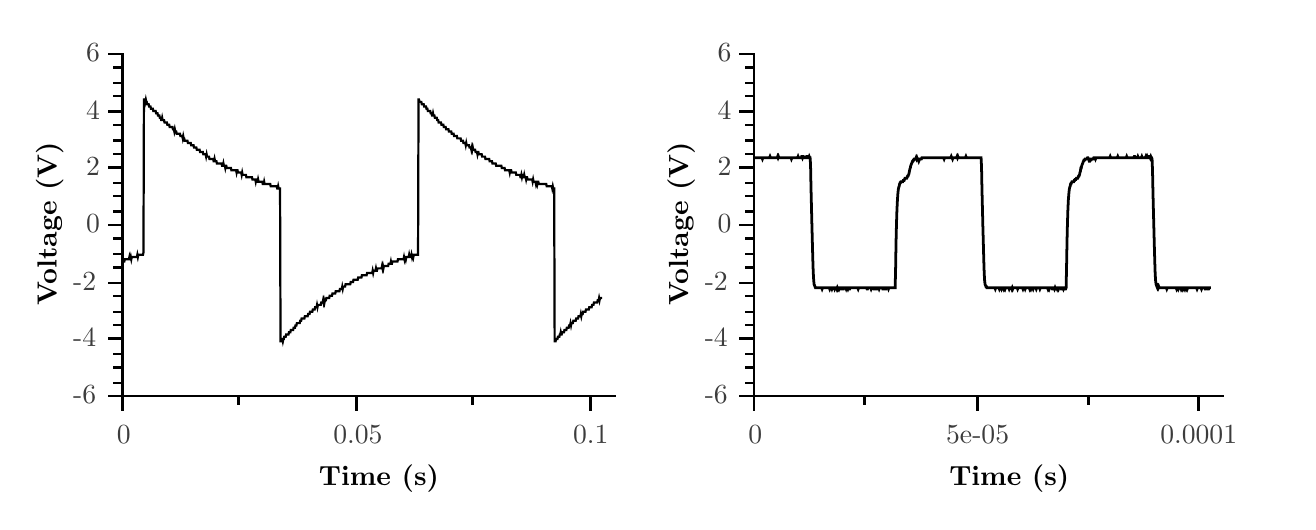
\begin{tikzpicture}{0pt}{0pt}{479pt}{180pt}
	\clip(0pt,180pt) -- (455.491pt,180pt) -- (455.491pt,8.83421pt) -- (0pt,8.83421pt) -- (0pt,180pt);
\begin{scope}
	\clip(262.454pt,170.491pt) -- (431.718pt,170.491pt) -- (431.718pt,46.8711pt) -- (262.454pt,46.8711pt) -- (262.454pt,170.491pt);
	\color[gray]{0}
	\draw[line width=1pt, line join=miter, line cap=rect](262.615pt,132.993pt) -- (262.776pt,132.993pt) -- (262.937pt,132.993pt) -- (263.098pt,132.993pt) -- (263.259pt,132.993pt) -- (263.42pt,132.993pt) -- (263.58pt,132.993pt) -- (263.741pt,132.993pt) -- (263.902pt,132.993pt) -- (264.063pt,132.993pt) -- (264.224pt,132.993pt) -- (264.385pt,132.993pt) -- (264.546pt,132.993pt) -- (264.707pt,132.993pt) -- (264.868pt,132.993pt) -- (265.029pt,132.993pt) -- (265.189pt,132.993pt) -- (265.35pt,132.993pt) -- (265.511pt,132.581pt) -- (265.672pt,132.993pt) -- (265.833pt,132.993pt) -- (265.994pt,132.993pt) -- (266.155pt,132.993pt) -- (266.316pt,132.993pt) -- (266.477pt,132.993pt) -- (266.638pt,132.993pt) -- (266.798pt,132.993pt) -- (266.959pt,132.993pt) -- (267.12pt,132.993pt) -- (267.281pt,132.993pt) -- (267.442pt,132.993pt) -- (267.603pt,132.993pt) -- (267.764pt,132.993pt) -- (267.925pt,132.993pt) -- (268.086pt,132.993pt) -- (268.247pt,133.405pt) -- (268.407pt,132.993pt) -- (268.568pt,132.993pt) -- (268.729pt,132.993pt) -- (268.89pt,132.993pt) -- (269.051pt,132.993pt) -- (269.212pt,132.993pt) -- (269.373pt,132.993pt) -- (269.534pt,132.993pt) -- (269.695pt,132.993pt) -- (269.855pt,132.993pt) -- (270.016pt,132.993pt) -- (270.177pt,132.993pt) -- (270.338pt,132.993pt) -- (270.499pt,132.993pt) -- (270.66pt,132.993pt) -- (270.821pt,132.993pt) -- (270.982pt,133.405pt) -- (271.143pt,132.993pt) -- (271.304pt,133.405pt) -- (271.464pt,132.993pt) -- (271.625pt,132.993pt) -- (271.786pt,132.993pt) -- (271.947pt,132.993pt) -- (272.108pt,132.993pt) -- (272.269pt,132.993pt) -- (272.43pt,132.993pt) -- (272.591pt,132.993pt) -- (272.752pt,132.993pt) -- (272.913pt,132.993pt) -- (273.073pt,132.993pt) -- (273.234pt,132.993pt) -- (273.395pt,132.993pt) -- (273.556pt,132.993pt) -- (273.717pt,132.993pt) -- (273.878pt,132.993pt) -- (274.039pt,132.993pt) -- (274.2pt,132.993pt) -- (274.361pt,132.993pt) -- (274.522pt,132.993pt) -- (274.682pt,132.993pt) -- (274.843pt,132.993pt) -- (275.004pt,132.993pt) -- (275.165pt,132.993pt) -- (275.326pt,132.993pt) -- (275.487pt,132.993pt) -- (275.648pt,132.993pt) -- (275.809pt,132.993pt) -- (275.97pt,132.581pt) -- (276.13pt,132.993pt) -- (276.291pt,132.993pt) -- (276.452pt,132.993pt) -- (276.613pt,132.993pt) -- (276.774pt,132.993pt) -- (276.935pt,132.993pt) -- (277.096pt,132.993pt) -- (277.257pt,132.993pt) -- (277.418pt,132.993pt) -- (277.579pt,132.993pt) -- (277.739pt,132.993pt) -- (277.9pt,132.993pt) -- (278.061pt,132.993pt) -- (278.222pt,132.993pt) -- (278.383pt,133.405pt) -- (278.544pt,132.993pt) -- (278.705pt,132.993pt) -- (278.866pt,132.993pt) -- (279.027pt,132.993pt) -- (279.188pt,132.993pt) -- (279.348pt,132.993pt) -- (279.509pt,132.993pt) -- (279.67pt,133.405pt) -- (279.831pt,133.405pt) -- (279.992pt,132.993pt) -- (280.153pt,133.405pt) -- (280.314pt,133.405pt) -- (280.475pt,132.993pt) -- (280.636pt,132.993pt) -- (280.797pt,132.993pt) -- (280.957pt,132.993pt) -- (281.118pt,132.993pt) -- (281.279pt,132.993pt) -- (281.44pt,133.405pt) -- (281.601pt,133.405pt) -- (281.762pt,133.405pt) -- (281.923pt,132.993pt) -- (282.084pt,132.993pt) -- (282.245pt,132.993pt) -- (282.405pt,133.405pt) -- (282.566pt,132.993pt) -- (282.727pt,132.993pt) -- (282.888pt,130.52pt) -- (283.049pt,122.279pt) -- (283.21pt,115.686pt) -- (283.371pt,109.093pt) -- (283.532pt,102.912pt) -- (283.693pt,96.731pt) -- (283.854pt,91.7862pt) -- (284.014pt,88.9018pt) -- (284.175pt,87.2535pt) -- (284.336pt,86.8414pt) -- (284.497pt,86.4294pt) -- (284.658pt,86.0173pt) -- (284.819pt,86.0173pt) -- (284.98pt,86.0173pt) -- (285.141pt,86.0173pt) -- (285.302pt,86.0173pt) -- (285.463pt,86.0173pt) -- (285.623pt,86.0173pt) -- (285.784pt,86.0173pt) -- (285.945pt,86.0173pt) -- (286.106pt,86.0173pt) -- (286.267pt,86.0173pt) -- (286.428pt,86.0173pt) -- (286.589pt,86.0173pt) -- (286.75pt,86.0173pt) -- (286.911pt,86.0173pt) -- (287.071pt,85.6052pt) -- (287.232pt,86.0173pt) -- (287.393pt,86.0173pt) -- (287.554pt,86.0173pt) -- (287.715pt,86.0173pt) -- (287.876pt,86.0173pt) -- (288.037pt,86.0173pt) -- (288.198pt,86.0173pt) -- (288.359pt,86.0173pt) -- (288.52pt,86.0173pt) -- (288.68pt,86.0173pt) -- (288.841pt,86.0173pt) -- (289.002pt,86.0173pt) -- (289.163pt,86.0173pt) -- (289.324pt,86.0173pt) -- (289.485pt,86.0173pt) -- (289.646pt,86.0173pt) -- (289.807pt,85.6052pt) -- (289.968pt,86.0173pt) -- (290.129pt,86.0173pt) -- (290.289pt,86.0173pt) -- (290.45pt,86.0173pt) -- (290.611pt,85.6052pt) -- (290.772pt,86.0173pt) -- (290.933pt,86.0173pt) -- (291.094pt,86.0173pt) -- (291.255pt,86.0173pt) -- (291.416pt,86.0173pt) -- (291.577pt,85.6052pt) -- (291.738pt,86.0173pt) -- (291.898pt,86.0173pt) -- (292.059pt,86.0173pt) -- (292.22pt,86.0173pt) -- (292.381pt,85.6052pt) -- (292.542pt,86.0173pt) -- (292.703pt,85.6052pt) -- (292.864pt,86.0173pt) -- (293.025pt,86.0173pt) -- (293.186pt,85.6052pt) -- (293.346pt,86.0173pt) -- (293.507pt,86.0173pt) -- (293.668pt,85.6052pt) -- (293.829pt,85.6052pt) -- (293.99pt,86.0173pt) -- (294.151pt,86.0173pt) -- (294.312pt,86.0173pt) -- (294.473pt,85.6052pt) -- (294.634pt,85.6052pt) -- (294.795pt,85.6052pt) -- (294.955pt,86.0173pt) -- (295.116pt,86.0173pt) -- (295.277pt,86.0173pt) -- (295.438pt,86.0173pt) -- (295.599pt,86.0173pt) -- (295.76pt,85.6052pt) -- (295.921pt,86.0173pt) -- (296.082pt,86.0173pt) -- (296.243pt,86.0173pt) -- (296.404pt,85.6052pt) -- (296.564pt,86.0173pt) -- (296.725pt,86.0173pt) -- (296.886pt,85.6052pt) -- (297.047pt,85.6052pt) -- (297.208pt,86.0173pt) -- (297.369pt,86.0173pt) -- (297.53pt,86.0173pt) -- (297.691pt,86.0173pt) -- (297.852pt,86.0173pt) -- (298.013pt,86.0173pt) -- (298.173pt,86.0173pt) -- (298.334pt,86.0173pt) -- (298.495pt,86.0173pt) -- (298.656pt,86.0173pt) -- (298.817pt,86.0173pt) -- (298.978pt,86.0173pt) -- (299.139pt,86.0173pt) -- (299.3pt,86.0173pt) -- (299.461pt,86.0173pt) -- (299.621pt,86.0173pt) -- (299.782pt,86.0173pt) -- (299.943pt,86.0173pt) -- (300.104pt,85.6052pt) -- (300.265pt,86.0173pt) -- (300.426pt,86.0173pt) -- (300.587pt,86.0173pt) -- (300.748pt,86.0173pt) -- (300.909pt,86.0173pt) -- (301.07pt,86.0173pt) -- (301.23pt,86.0173pt) -- (301.391pt,86.0173pt) -- (301.552pt,86.0173pt) -- (301.713pt,86.0173pt) -- (301.874pt,86.0173pt) -- (302.035pt,86.0173pt) -- (302.196pt,86.0173pt) -- (302.357pt,86.0173pt) -- (302.518pt,86.0173pt) -- (302.679pt,86.0173pt) -- (302.839pt,86.0173pt) -- (303pt,86.0173pt) -- (303.161pt,86.0173pt) -- (303.322pt,85.6052pt) -- (303.483pt,85.6052pt) -- (303.644pt,86.0173pt) -- (303.805pt,86.0173pt) -- (303.966pt,86.0173pt) -- (304.127pt,86.0173pt) -- (304.288pt,86.0173pt) -- (304.448pt,86.0173pt) -- (304.609pt,86.0173pt) -- (304.77pt,85.6052pt) -- (304.931pt,86.0173pt) -- (305.092pt,86.0173pt) -- (305.253pt,86.0173pt) -- (305.414pt,86.0173pt) -- (305.575pt,86.0173pt) -- (305.736pt,85.6052pt) -- (305.896pt,85.6052pt) -- (306.057pt,86.0173pt) -- (306.218pt,86.0173pt) -- (306.379pt,86.0173pt) -- (306.54pt,86.0173pt) -- (306.701pt,85.6052pt) -- (306.862pt,85.6052pt) -- (307.023pt,86.0173pt) -- (307.184pt,86.0173pt) -- (307.345pt,86.0173pt) -- (307.505pt,86.0173pt) -- (307.666pt,85.6052pt) -- (307.827pt,86.0173pt) -- (307.988pt,86.0173pt) -- (308.149pt,86.0173pt) -- (308.31pt,86.0173pt) -- (308.471pt,86.0173pt) -- (308.632pt,86.0173pt) -- (308.793pt,86.0173pt) -- (308.954pt,85.6052pt) -- (309.114pt,85.6052pt) -- (309.275pt,85.6052pt) -- (309.436pt,86.0173pt) -- (309.597pt,86.0173pt) -- (309.758pt,86.0173pt) -- (309.919pt,85.6052pt) -- (310.08pt,85.6052pt) -- (310.241pt,86.0173pt) -- (310.402pt,86.0173pt) -- (310.562pt,86.0173pt) -- (310.723pt,86.0173pt) -- (310.884pt,86.0173pt) -- (311.045pt,85.6052pt) -- (311.206pt,86.0173pt) -- (311.367pt,86.0173pt) -- (311.528pt,86.0173pt) -- (311.689pt,86.0173pt) -- (311.85pt,86.0173pt) -- (312.011pt,86.0173pt) -- (312.171pt,86.0173pt) -- (312.332pt,86.0173pt) -- (312.493pt,86.0173pt) -- (312.654pt,86.0173pt) -- (312.815pt,86.0173pt) -- (312.976pt,86.0173pt) -- (313.137pt,86.0173pt) -- (313.298pt,86.0173pt) -- (313.459pt,86.0173pt) -- (313.62pt,92.6104pt) -- (313.78pt,102.5pt) -- (313.941pt,109.093pt) -- (314.102pt,114.038pt) -- (314.263pt,117.334pt) -- (314.424pt,119.807pt) -- (314.585pt,121.455pt) -- (314.746pt,122.279pt) -- (314.907pt,122.691pt) -- (315.068pt,123.515pt) -- (315.229pt,123.927pt) -- (315.389pt,123.927pt) -- (315.55pt,124.339pt) -- (315.711pt,124.339pt) -- (315.872pt,124.339pt) -- (316.033pt,124.339pt) -- (316.194pt,124.339pt) -- (316.355pt,124.751pt) -- (316.516pt,124.751pt) -- (316.677pt,124.751pt) -- (316.837pt,125.164pt) -- (316.998pt,125.576pt) -- (317.159pt,125.576pt) -- (317.32pt,125.576pt) -- (317.481pt,125.576pt) -- (317.642pt,125.576pt) -- (317.803pt,125.988pt) -- (317.964pt,126.4pt) -- (318.125pt,126.4pt) -- (318.286pt,126.812pt) -- (318.446pt,127.224pt) -- (318.607pt,128.048pt) -- (318.768pt,128.872pt) -- (318.929pt,129.284pt) -- (319.09pt,130.108pt) -- (319.251pt,130.52pt) -- (319.412pt,130.932pt) -- (319.573pt,131.345pt) -- (319.734pt,131.757pt) -- (319.895pt,131.757pt) -- (320.055pt,132.169pt) -- (320.216pt,132.169pt) -- (320.377pt,132.581pt) -- (320.538pt,132.581pt) -- (320.699pt,132.581pt) -- (320.86pt,132.581pt) -- (321.021pt,132.993pt) -- (321.182pt,132.581pt) -- (321.343pt,132.993pt) -- (321.504pt,132.581pt) -- (321.664pt,132.581pt) -- (321.825pt,132.169pt) -- (321.986pt,131.757pt) -- (322.147pt,132.169pt) -- (322.308pt,132.581pt) -- (322.469pt,132.581pt) -- (322.63pt,132.581pt) -- (322.791pt,132.581pt) -- (322.952pt,132.581pt) -- (323.112pt,132.993pt) -- (323.273pt,132.993pt) -- (323.434pt,132.993pt) -- (323.595pt,132.993pt) -- (323.756pt,132.993pt) -- (323.917pt,132.993pt) -- (324.078pt,132.993pt) -- (324.239pt,132.993pt) -- (324.4pt,132.993pt) -- (324.561pt,132.993pt) -- (324.721pt,132.993pt) -- (324.882pt,132.993pt) -- (325.043pt,132.993pt) -- (325.204pt,132.993pt) -- (325.365pt,132.993pt) -- (325.526pt,132.993pt) -- (325.687pt,132.993pt) -- (325.848pt,132.993pt) -- (326.009pt,132.993pt) -- (326.17pt,132.993pt) -- (326.33pt,132.993pt) -- (326.491pt,132.993pt) -- (326.652pt,132.993pt) -- (326.813pt,132.993pt) -- (326.974pt,132.993pt) -- (327.135pt,132.993pt) -- (327.296pt,132.993pt) -- (327.457pt,132.993pt) -- (327.618pt,132.993pt) -- (327.779pt,132.993pt) -- (327.939pt,132.993pt) -- (328.1pt,132.993pt) -- (328.261pt,132.993pt) -- (328.422pt,132.993pt) -- (328.583pt,132.993pt) -- (328.744pt,132.993pt) -- (328.905pt,132.993pt) -- (329.066pt,132.993pt) -- (329.227pt,132.993pt) -- (329.387pt,132.993pt) -- (329.548pt,132.993pt) -- (329.709pt,132.993pt) -- (329.87pt,132.993pt) -- (330.031pt,132.993pt) -- (330.192pt,132.993pt) -- (330.353pt,132.993pt) -- (330.514pt,132.993pt) -- (330.675pt,132.993pt) -- (330.836pt,132.993pt) -- (330.996pt,132.993pt) -- (331.157pt,132.581pt) -- (331.318pt,132.993pt) -- (331.479pt,132.993pt) -- (331.64pt,132.993pt) -- (331.801pt,132.993pt) -- (331.962pt,132.993pt) -- (332.123pt,132.993pt) -- (332.284pt,132.993pt) -- (332.445pt,132.993pt) -- (332.605pt,132.993pt) -- (332.766pt,132.993pt) -- (332.927pt,132.993pt) -- (333.088pt,132.993pt) -- (333.249pt,132.993pt) -- (333.41pt,132.993pt) -- (333.571pt,132.993pt) -- (333.732pt,133.405pt) -- (333.893pt,132.993pt) -- (334.054pt,132.993pt) -- (334.214pt,132.581pt) -- (334.375pt,132.993pt) -- (334.536pt,132.993pt) -- (334.697pt,132.993pt) -- (334.858pt,132.993pt) -- (335.019pt,132.993pt) -- (335.18pt,132.993pt) -- (335.341pt,132.993pt) -- (335.502pt,132.993pt) -- (335.662pt,132.993pt) -- (335.823pt,133.405pt) -- (335.984pt,132.993pt) -- (336.145pt,133.405pt) -- (336.306pt,132.993pt) -- (336.467pt,132.993pt) -- (336.628pt,132.993pt) -- (336.789pt,132.993pt) -- (336.95pt,132.993pt) -- (337.111pt,132.993pt) -- (337.271pt,132.993pt) -- (337.432pt,132.993pt) -- (337.593pt,132.993pt) -- (337.754pt,132.993pt) -- (337.915pt,132.993pt) -- (338.076pt,132.993pt) -- (338.237pt,132.993pt) -- (338.398pt,132.993pt) -- (338.559pt,132.993pt) -- (338.72pt,132.993pt) -- (338.88pt,132.993pt) -- (339.041pt,133.405pt) -- (339.202pt,132.993pt) -- (339.363pt,132.993pt) -- (339.524pt,132.993pt) -- (339.685pt,132.993pt) -- (339.846pt,132.993pt) -- (340.007pt,132.993pt) -- (340.168pt,132.993pt) -- (340.328pt,132.993pt) -- (340.489pt,132.993pt) -- (340.65pt,132.993pt) -- (340.811pt,132.993pt) -- (340.972pt,132.993pt) -- (341.133pt,132.993pt) -- (341.294pt,132.993pt) -- (341.455pt,132.993pt) -- (341.616pt,132.993pt) -- (341.777pt,132.993pt) -- (341.937pt,132.993pt) -- (342.098pt,132.993pt) -- (342.259pt,132.993pt) -- (342.42pt,132.993pt) -- (342.581pt,132.993pt) -- (342.742pt,132.993pt) -- (342.903pt,132.993pt) -- (343.064pt,132.993pt) -- (343.225pt,132.993pt) -- (343.386pt,132.993pt) -- (343.546pt,132.993pt) -- (343.707pt,132.993pt) -- (343.868pt,132.993pt) -- (344.029pt,132.993pt) -- (344.19pt,132.993pt) -- (344.351pt,132.993pt) -- (344.512pt,132.993pt) -- (344.673pt,129.696pt) -- (344.834pt,121.455pt) -- (344.995pt,114.862pt) -- (345.155pt,108.269pt) -- (345.316pt,102.5pt) -- (345.477pt,96.3189pt) -- (345.638pt,91.3742pt) -- (345.799pt,88.4897pt) -- (345.96pt,87.2535pt) -- (346.121pt,86.8414pt) -- (346.282pt,86.4294pt) -- (346.443pt,86.4294pt) -- (346.603pt,86.0173pt) -- (346.764pt,86.0173pt) -- (346.925pt,86.0173pt) -- (347.086pt,86.0173pt) -- (347.247pt,86.0173pt) -- (347.408pt,86.0173pt) -- (347.569pt,86.0173pt) -- (347.73pt,86.0173pt) -- (347.891pt,86.0173pt) -- (348.052pt,86.0173pt) -- (348.212pt,86.0173pt) -- (348.373pt,86.0173pt) -- (348.534pt,86.0173pt) -- (348.695pt,86.0173pt) -- (348.856pt,86.0173pt) -- (349.017pt,86.0173pt) -- (349.178pt,86.0173pt) -- (349.339pt,86.0173pt) -- (349.5pt,86.0173pt) -- (349.661pt,85.6052pt) -- (349.821pt,86.0173pt) -- (349.982pt,86.0173pt) -- (350.143pt,86.0173pt) -- (350.304pt,86.0173pt) -- (350.465pt,86.0173pt) -- (350.626pt,86.0173pt) -- (350.787pt,86.0173pt) -- (350.948pt,86.0173pt) -- (351.109pt,85.6052pt) -- (351.27pt,86.0173pt) -- (351.43pt,86.0173pt) -- (351.591pt,86.0173pt) -- (351.752pt,86.0173pt) -- (351.913pt,85.6052pt) -- (352.074pt,86.0173pt) -- (352.235pt,86.0173pt) -- (352.396pt,86.0173pt) -- (352.557pt,86.0173pt) -- (352.718pt,85.6052pt) -- (352.878pt,86.0173pt) -- (353.039pt,86.0173pt) -- (353.2pt,85.6052pt) -- (353.361pt,86.0173pt) -- (353.522pt,86.0173pt) -- (353.683pt,86.0173pt) -- (353.844pt,86.0173pt) -- (354.005pt,86.0173pt) -- (354.166pt,86.0173pt) -- (354.327pt,86.0173pt) -- (354.487pt,86.0173pt) -- (354.648pt,85.6052pt) -- (354.809pt,86.0173pt) -- (354.97pt,86.0173pt) -- (355.131pt,86.0173pt) -- (355.292pt,86.0173pt) -- (355.453pt,86.0173pt) -- (355.614pt,85.6052pt) -- (355.775pt,86.0173pt) -- (355.936pt,85.6052pt) -- (356.096pt,86.0173pt) -- (356.257pt,86.0173pt) -- (356.418pt,86.0173pt) -- (356.579pt,86.0173pt) -- (356.74pt,86.0173pt) -- (356.901pt,86.0173pt) -- (357.062pt,86.0173pt) -- (357.223pt,86.0173pt) -- (357.384pt,86.0173pt) -- (357.545pt,86.0173pt) -- (357.705pt,85.6052pt) -- (357.866pt,86.0173pt) -- (358.027pt,86.0173pt) -- (358.188pt,86.0173pt) -- (358.349pt,86.0173pt) -- (358.51pt,86.0173pt) -- (358.671pt,86.0173pt) -- (358.832pt,86.0173pt) -- (358.993pt,86.0173pt) -- (359.153pt,86.0173pt) -- (359.314pt,86.0173pt) -- (359.475pt,86.0173pt) -- (359.636pt,85.6052pt) -- (359.797pt,86.0173pt) -- (359.958pt,86.0173pt) -- (360.119pt,86.0173pt) -- (360.28pt,86.0173pt) -- (360.441pt,85.6052pt) -- (360.602pt,86.0173pt) -- (360.762pt,86.0173pt) -- (360.923pt,86.0173pt) -- (361.084pt,86.0173pt) -- (361.245pt,86.0173pt) -- (361.406pt,86.0173pt) -- (361.567pt,86.0173pt) -- (361.728pt,86.0173pt) -- (361.889pt,86.0173pt) -- (362.05pt,85.6052pt) -- (362.211pt,86.0173pt) -- (362.371pt,86.0173pt) -- (362.532pt,85.6052pt) -- (362.693pt,86.0173pt) -- (362.854pt,86.0173pt) -- (363.015pt,86.0173pt) -- (363.176pt,86.0173pt) -- (363.337pt,85.6052pt) -- (363.498pt,86.0173pt) -- (363.659pt,86.0173pt) -- (363.82pt,86.0173pt) -- (363.98pt,86.0173pt) -- (364.141pt,86.0173pt) -- (364.302pt,86.0173pt) -- (364.463pt,85.6052pt) -- (364.624pt,86.0173pt) -- (364.785pt,86.0173pt) -- (364.946pt,86.0173pt) -- (365.107pt,86.0173pt) -- (365.268pt,86.0173pt) -- (365.428pt,86.0173pt) -- (365.589pt,86.0173pt) -- (365.75pt,85.6052pt) -- (365.911pt,86.0173pt) -- (366.072pt,86.0173pt) -- (366.233pt,86.0173pt) -- (366.394pt,86.0173pt) -- (366.555pt,86.0173pt) -- (366.716pt,86.0173pt) -- (366.877pt,86.0173pt) -- (367.037pt,86.0173pt) -- (367.198pt,86.0173pt) -- (367.359pt,86.0173pt) -- (367.52pt,86.0173pt) -- (367.681pt,86.0173pt) -- (367.842pt,86.0173pt) -- (368.003pt,86.0173pt) -- (368.164pt,86.0173pt) -- (368.325pt,86.0173pt) -- (368.486pt,86.0173pt) -- (368.646pt,85.6052pt) -- (368.807pt,86.0173pt) -- (368.968pt,86.0173pt) -- (369.129pt,85.6052pt) -- (369.29pt,86.0173pt) -- (369.451pt,86.0173pt) -- (369.612pt,86.0173pt) -- (369.773pt,86.0173pt) -- (369.934pt,86.0173pt) -- (370.094pt,86.0173pt) -- (370.255pt,85.6052pt) -- (370.416pt,85.6052pt) -- (370.577pt,86.0173pt) -- (370.738pt,86.0173pt) -- (370.899pt,86.0173pt) -- (371.06pt,85.6052pt) -- (371.221pt,86.0173pt) -- (371.382pt,85.6052pt) -- (371.543pt,85.6052pt) -- (371.703pt,86.0173pt) -- (371.864pt,86.0173pt) -- (372.025pt,85.6052pt) -- (372.186pt,86.0173pt) -- (372.347pt,86.0173pt) -- (372.508pt,85.6052pt) -- (372.669pt,86.0173pt) -- (372.83pt,86.0173pt) -- (372.991pt,86.0173pt) -- (373.152pt,86.0173pt) -- (373.312pt,86.0173pt) -- (373.473pt,85.6052pt) -- (373.634pt,85.6052pt) -- (373.795pt,86.0173pt) -- (373.956pt,86.0173pt) -- (374.117pt,86.0173pt) -- (374.278pt,85.6052pt) -- (374.439pt,86.0173pt) -- (374.6pt,86.0173pt) -- (374.761pt,86.0173pt) -- (374.921pt,85.6052pt) -- (375.082pt,85.6052pt) -- (375.243pt,86.0173pt) -- (375.404pt,93.8466pt) -- (375.565pt,102.912pt) -- (375.726pt,109.505pt) -- (375.887pt,114.45pt) -- (376.048pt,117.746pt) -- (376.209pt,119.807pt) -- (376.369pt,121.455pt) -- (376.53pt,122.279pt) -- (376.691pt,122.691pt) -- (376.852pt,123.515pt) -- (377.013pt,123.515pt) -- (377.174pt,123.927pt) -- (377.335pt,124.339pt) -- (377.496pt,124.339pt) -- (377.657pt,124.339pt) -- (377.818pt,124.339pt) -- (377.978pt,124.339pt) -- (378.139pt,124.751pt) -- (378.3pt,124.751pt) -- (378.461pt,125.164pt) -- (378.622pt,125.164pt) -- (378.783pt,125.164pt) -- (378.944pt,125.576pt) -- (379.105pt,125.576pt) -- (379.266pt,125.576pt) -- (379.427pt,125.576pt) -- (379.587pt,125.988pt) -- (379.748pt,126.4pt) -- (379.909pt,126.4pt) -- (380.07pt,126.812pt) -- (380.231pt,127.636pt) -- (380.392pt,128.048pt) -- (380.553pt,129.284pt) -- (380.714pt,129.284pt) -- (380.875pt,130.108pt) -- (381.036pt,130.52pt) -- (381.196pt,130.932pt) -- (381.357pt,131.345pt) -- (381.518pt,131.757pt) -- (381.679pt,132.169pt) -- (381.84pt,132.169pt) -- (382.001pt,132.169pt) -- (382.162pt,132.581pt) -- (382.323pt,132.581pt) -- (382.484pt,132.581pt) -- (382.644pt,132.581pt) -- (382.805pt,132.581pt) -- (382.966pt,132.993pt) -- (383.127pt,132.993pt) -- (383.288pt,132.581pt) -- (383.449pt,132.581pt) -- (383.61pt,131.757pt) -- (383.771pt,131.757pt) -- (383.932pt,132.169pt) -- (384.093pt,132.169pt) -- (384.253pt,132.169pt) -- (384.414pt,132.581pt) -- (384.575pt,132.581pt) -- (384.736pt,132.581pt) -- (384.897pt,132.581pt) -- (385.058pt,132.581pt) -- (385.219pt,132.993pt) -- (385.38pt,132.993pt) -- (385.541pt,132.993pt) -- (385.702pt,132.993pt) -- (385.862pt,132.581pt) -- (386.023pt,132.993pt) -- (386.184pt,132.993pt) -- (386.345pt,132.993pt) -- (386.506pt,132.993pt) -- (386.667pt,132.993pt) -- (386.828pt,132.993pt) -- (386.989pt,132.993pt) -- (387.15pt,132.993pt) -- (387.311pt,132.993pt) -- (387.471pt,132.993pt) -- (387.632pt,132.993pt) -- (387.793pt,132.993pt) -- (387.954pt,132.993pt) -- (388.115pt,132.993pt) -- (388.276pt,132.993pt) -- (388.437pt,132.993pt) -- (388.598pt,132.993pt) -- (388.759pt,132.993pt) -- (388.919pt,132.993pt) -- (389.08pt,132.993pt) -- (389.241pt,132.993pt) -- (389.402pt,132.993pt) -- (389.563pt,132.993pt) -- (389.724pt,132.993pt) -- (389.885pt,132.993pt) -- (390.046pt,132.993pt) -- (390.207pt,132.993pt) -- (390.368pt,132.993pt) -- (390.528pt,132.993pt) -- (390.689pt,132.993pt) -- (390.85pt,132.993pt) -- (391.011pt,132.993pt) -- (391.172pt,133.405pt) -- (391.333pt,132.993pt) -- (391.494pt,132.993pt) -- (391.655pt,132.993pt) -- (391.816pt,132.993pt) -- (391.977pt,132.993pt) -- (392.137pt,132.993pt) -- (392.298pt,132.993pt) -- (392.459pt,132.993pt) -- (392.62pt,132.993pt) -- (392.781pt,132.993pt) -- (392.942pt,132.993pt) -- (393.103pt,132.993pt) -- (393.264pt,132.993pt) -- (393.425pt,132.993pt) -- (393.586pt,132.993pt) -- (393.746pt,132.993pt) -- (393.907pt,133.405pt) -- (394.068pt,132.993pt) -- (394.229pt,132.993pt) -- (394.39pt,132.993pt) -- (394.551pt,132.993pt) -- (394.712pt,132.993pt) -- (394.873pt,132.993pt) -- (395.034pt,132.993pt) -- (395.194pt,132.993pt) -- (395.355pt,132.993pt) -- (395.516pt,132.993pt) -- (395.677pt,132.993pt) -- (395.838pt,132.993pt) -- (395.999pt,132.993pt) -- (396.16pt,132.993pt) -- (396.321pt,132.993pt) -- (396.482pt,132.993pt) -- (396.643pt,132.993pt) -- (396.803pt,132.993pt) -- (396.964pt,132.993pt) -- (397.125pt,133.405pt) -- (397.286pt,132.993pt) -- (397.447pt,132.993pt) -- (397.608pt,132.993pt) -- (397.769pt,132.993pt) -- (397.93pt,132.993pt) -- (398.091pt,132.993pt) -- (398.252pt,132.993pt) -- (398.412pt,132.993pt) -- (398.573pt,132.993pt) -- (398.734pt,132.993pt) -- (398.895pt,132.993pt) -- (399.056pt,132.993pt) -- (399.217pt,132.993pt) -- (399.378pt,132.993pt) -- (399.539pt,132.993pt) -- (399.7pt,132.993pt) -- (399.86pt,133.405pt) -- (400.021pt,133.405pt) -- (400.182pt,132.993pt) -- (400.343pt,132.993pt) -- (400.504pt,132.993pt) -- (400.665pt,132.993pt) -- (400.826pt,132.993pt) -- (400.987pt,132.993pt) -- (401.148pt,133.405pt) -- (401.309pt,132.993pt) -- (401.469pt,132.993pt) -- (401.63pt,132.993pt) -- (401.791pt,132.993pt) -- (401.952pt,132.993pt) -- (402.113pt,132.993pt) -- (402.274pt,132.993pt) -- (402.435pt,132.993pt) -- (402.596pt,133.405pt) -- (402.757pt,132.993pt) -- (402.918pt,132.993pt) -- (403.078pt,132.993pt) -- (403.239pt,132.993pt) -- (403.4pt,132.993pt) -- (403.561pt,132.993pt) -- (403.722pt,132.993pt) -- (403.883pt,132.993pt) -- (404.044pt,133.405pt) -- (404.205pt,132.993pt) -- (404.366pt,132.993pt) -- (404.527pt,133.405pt) -- (404.687pt,132.993pt) -- (404.848pt,132.993pt) -- (405.009pt,132.993pt) -- (405.17pt,133.405pt) -- (405.331pt,133.405pt) -- (405.492pt,133.405pt) -- (405.653pt,132.993pt) -- (405.814pt,133.405pt) -- (405.975pt,132.993pt) -- (406.135pt,132.993pt) -- (406.296pt,132.581pt) -- (406.457pt,128.46pt) -- (406.618pt,120.631pt) -- (406.779pt,114.038pt) -- (406.94pt,107.857pt) -- (407.101pt,101.676pt) -- (407.262pt,95.9069pt) -- (407.423pt,90.9621pt) -- (407.584pt,88.4897pt) -- (407.744pt,87.2535pt) -- (407.905pt,86.8414pt) -- (408.066pt,86.4294pt) -- (408.227pt,86.0173pt) -- (408.388pt,86.4294pt) -- (408.549pt,86.0173pt) -- (408.71pt,86.4294pt) -- (408.871pt,86.0173pt) -- (409.032pt,86.0173pt) -- (409.193pt,86.0173pt) -- (409.353pt,86.0173pt) -- (409.514pt,86.0173pt) -- (409.675pt,86.0173pt) -- (409.836pt,86.0173pt) -- (409.997pt,86.0173pt) -- (410.158pt,86.0173pt) -- (410.319pt,86.0173pt) -- (410.48pt,86.0173pt) -- (410.641pt,86.0173pt) -- (410.802pt,86.0173pt) -- (410.962pt,86.0173pt) -- (411.123pt,86.0173pt) -- (411.284pt,86.0173pt) -- (411.445pt,86.0173pt) -- (411.606pt,85.6052pt) -- (411.767pt,86.0173pt) -- (411.928pt,86.0173pt) -- (412.089pt,86.0173pt) -- (412.25pt,86.0173pt) -- (412.41pt,86.0173pt) -- (412.571pt,86.0173pt) -- (412.732pt,86.0173pt) -- (412.893pt,86.0173pt) -- (413.054pt,86.0173pt) -- (413.215pt,86.0173pt) -- (413.376pt,86.0173pt) -- (413.537pt,86.0173pt) -- (413.698pt,86.0173pt) -- (413.859pt,86.0173pt) -- (414.019pt,86.0173pt) -- (414.18pt,86.0173pt) -- (414.341pt,86.0173pt) -- (414.502pt,86.0173pt) -- (414.663pt,86.0173pt) -- (414.824pt,86.0173pt) -- (414.985pt,86.0173pt) -- (415.146pt,85.6052pt) -- (415.307pt,86.0173pt) -- (415.468pt,86.0173pt) -- (415.628pt,86.0173pt) -- (415.789pt,85.6052pt) -- (415.95pt,86.0173pt) -- (416.111pt,86.0173pt) -- (416.272pt,86.0173pt) -- (416.433pt,86.0173pt) -- (416.594pt,86.0173pt) -- (416.755pt,85.6052pt) -- (416.916pt,86.0173pt) -- (417.077pt,86.0173pt) -- (417.237pt,85.6052pt) -- (417.398pt,86.0173pt) -- (417.559pt,86.0173pt) -- (417.72pt,86.0173pt) -- (417.881pt,85.6052pt) -- (418.042pt,86.0173pt) -- (418.203pt,86.0173pt) -- (418.364pt,86.0173pt) -- (418.525pt,85.6052pt) -- (418.685pt,86.0173pt) -- (418.846pt,86.0173pt) -- (419.007pt,85.6052pt) -- (419.168pt,86.0173pt) -- (419.329pt,86.0173pt) -- (419.49pt,86.0173pt) -- (419.651pt,86.0173pt) -- (419.812pt,86.0173pt) -- (419.973pt,86.0173pt) -- (420.134pt,86.0173pt) -- (420.294pt,86.0173pt) -- (420.455pt,86.0173pt) -- (420.616pt,86.0173pt) -- (420.777pt,86.0173pt) -- (420.938pt,86.0173pt) -- (421.099pt,86.0173pt) -- (421.26pt,86.0173pt) -- (421.421pt,86.0173pt) -- (421.582pt,86.0173pt) -- (421.743pt,86.0173pt) -- (421.903pt,86.0173pt) -- (422.064pt,86.0173pt) -- (422.225pt,86.0173pt) -- (422.386pt,86.0173pt) -- (422.547pt,85.6052pt) -- (422.708pt,86.0173pt) -- (422.869pt,86.0173pt) -- (423.03pt,86.0173pt) -- (423.191pt,86.0173pt) -- (423.351pt,86.0173pt) -- (423.512pt,86.0173pt) -- (423.673pt,86.0173pt) -- (423.834pt,86.0173pt) -- (423.995pt,86.0173pt) -- (424.156pt,85.6052pt) -- (424.317pt,86.0173pt) -- (424.478pt,86.0173pt) -- (424.639pt,86.0173pt) -- (424.8pt,86.0173pt) -- (424.96pt,86.0173pt) -- (425.121pt,86.0173pt) -- (425.282pt,86.0173pt) -- (425.443pt,85.6052pt) -- (425.604pt,85.6052pt) -- (425.765pt,86.0173pt) -- (425.926pt,86.0173pt) -- (426.087pt,86.0173pt) -- (426.248pt,86.0173pt) -- (426.409pt,85.6052pt) -- (426.569pt,85.6052pt) -- (426.73pt,85.6052pt) -- (426.891pt,86.0173pt) -- (427.052pt,86.0173pt);
\end{scope}
\begin{scope}
	\color[gray]{0}
	\pgftext[center, base, at={\pgfpoint{238.681pt}{109.156pt}},rotate=90]{\textbf{Voltage (V)}}
	\color[gray]{0.235294}
	\pgftext[center, base, at={\pgfpoint{248.829pt}{44.0183pt}}]{-6}
	\pgftext[center, base, at={\pgfpoint{248.829pt}{64.9386pt}}]{-4}
	\pgftext[center, base, at={\pgfpoint{248.829pt}{84.9079pt}}]{-2}
	\pgftext[center, base, at={\pgfpoint{251.838pt}{105.828pt}}]{0}
	\pgftext[center, base, at={\pgfpoint{251.838pt}{126.748pt}}]{2}
	\pgftext[center, base, at={\pgfpoint{251.838pt}{146.718pt}}]{4}
	\pgftext[center, base, at={\pgfpoint{251.838pt}{167.638pt}}]{6}
	\color[gray]{0}
	\draw[line width=1pt, line join=bevel, line cap=rect](262.454pt,51.6257pt) -- (259.601pt,51.6257pt);
	\draw[line width=1pt, line join=bevel, line cap=rect](262.454pt,62.0858pt) -- (259.601pt,62.0858pt);
	\draw[line width=1pt, line join=bevel, line cap=rect](262.454pt,72.5459pt) -- (259.601pt,72.5459pt);
	\draw[line width=1pt, line join=bevel, line cap=rect](262.454pt,83.0061pt) -- (259.601pt,83.0061pt);
	\draw[line width=1pt, line join=bevel, line cap=rect](262.454pt,93.4662pt) -- (259.601pt,93.4662pt);
	\draw[line width=1pt, line join=bevel, line cap=rect](262.454pt,103.926pt) -- (259.601pt,103.926pt);
	\draw[line width=1pt, line join=bevel, line cap=rect](262.454pt,113.436pt) -- (259.601pt,113.436pt);
	\draw[line width=1pt, line join=bevel, line cap=rect](262.454pt,123.896pt) -- (259.601pt,123.896pt);
	\draw[line width=1pt, line join=bevel, line cap=rect](262.454pt,134.356pt) -- (259.601pt,134.356pt);
	\draw[line width=1pt, line join=bevel, line cap=rect](262.454pt,144.816pt) -- (259.601pt,144.816pt);
	\draw[line width=1pt, line join=bevel, line cap=rect](262.454pt,155.276pt) -- (259.601pt,155.276pt);
	\draw[line width=1pt, line join=bevel, line cap=rect](262.454pt,165.736pt) -- (259.601pt,165.736pt);
	\draw[line width=1pt, line join=bevel, line cap=rect](262.454pt,57.3312pt) -- (259.601pt,57.3312pt);
	\draw[line width=1pt, line join=bevel, line cap=rect](262.454pt,77.3005pt) -- (259.601pt,77.3005pt);
	\draw[line width=1pt, line join=bevel, line cap=rect](262.454pt,98.2208pt) -- (259.601pt,98.2208pt);
	\draw[line width=1pt, line join=bevel, line cap=rect](262.454pt,119.141pt) -- (259.601pt,119.141pt);
	\draw[line width=1pt, line join=bevel, line cap=rect](262.454pt,139.11pt) -- (259.601pt,139.11pt);
	\draw[line width=1pt, line join=bevel, line cap=rect](262.454pt,160.031pt) -- (259.601pt,160.031pt);
	\draw[line width=1pt, line join=bevel, line cap=rect](262.454pt,46.8711pt) -- (257.7pt,46.8711pt);
	\draw[line width=1pt, line join=bevel, line cap=rect](262.454pt,67.7913pt) -- (257.7pt,67.7913pt);
	\draw[line width=1pt, line join=bevel, line cap=rect](262.454pt,87.7607pt) -- (257.7pt,87.7607pt);
	\draw[line width=1pt, line join=bevel, line cap=rect](262.454pt,108.681pt) -- (257.7pt,108.681pt);
	\draw[line width=1pt, line join=bevel, line cap=rect](262.454pt,129.601pt) -- (257.7pt,129.601pt);
	\draw[line width=1pt, line join=bevel, line cap=rect](262.454pt,149.571pt) -- (257.7pt,149.571pt);
	\draw[line width=1pt, line join=bevel, line cap=rect](262.454pt,170.491pt) -- (257.7pt,170.491pt);
	\draw[line width=1pt, line join=bevel, line cap=rect](262.454pt,170.491pt) -- (262.454pt,46.8711pt);
	\pgftext[center, base, at={\pgfpoint{354.694pt}{14.5397pt}}]{\textbf{Time (s)}}
	\color[gray]{0.235294}
	\pgftext[center, base, at={\pgfpoint{262.922pt}{29.7545pt}}]{0}
	\pgftext[center, base, at={\pgfpoint{343.275pt}{29.7545pt}}]{5e-05}
	\pgftext[center, base, at={\pgfpoint{423.152pt}{29.7545pt}}]{0.0001}
	\color[gray]{0}
	\draw[line width=1pt, line join=bevel, line cap=rect](302.393pt,46.8711pt) -- (302.393pt,44.0183pt);
	\draw[line width=1pt, line join=bevel, line cap=rect](383.221pt,46.8711pt) -- (383.221pt,44.0183pt);
	\draw[line width=1pt, line join=bevel, line cap=rect](262.454pt,46.8711pt) -- (262.454pt,42.1164pt);
	\draw[line width=1pt, line join=bevel, line cap=rect](343.282pt,46.8711pt) -- (343.282pt,42.1164pt);
	\draw[line width=1pt, line join=bevel, line cap=rect](423.16pt,46.8711pt) -- (423.16pt,42.1164pt);
	\draw[line width=1pt, line join=bevel, line cap=rect](262.454pt,46.8711pt) -- (431.718pt,46.8711pt);
\end{scope}
\begin{scope}
	\clip(34.2332pt,170.491pt) -- (212.055pt,170.491pt) -- (212.055pt,46.8711pt) -- (34.2332pt,46.8711pt) -- (34.2332pt,170.491pt);
	\color[gray]{0}
	\draw[line width=0.8pt, line join=miter, line cap=rect](34.4022pt,95.4948pt) -- (34.5712pt,95.4948pt) -- (34.7403pt,95.4948pt) -- (34.9093pt,95.4948pt) -- (35.0783pt,96.3189pt) -- (35.2474pt,96.3189pt) -- (35.4164pt,96.3189pt) -- (35.5854pt,96.3189pt) -- (35.7545pt,96.3189pt) -- (35.9235pt,96.3189pt) -- (36.0925pt,96.3189pt) -- (36.2615pt,96.3189pt) -- (36.4306pt,96.3189pt) -- (36.5996pt,96.3189pt) -- (36.7686pt,97.1431pt) -- (36.9377pt,96.3189pt) -- (37.1067pt,96.3189pt) -- (37.2757pt,97.1431pt) -- (37.4448pt,96.3189pt) -- (37.6138pt,97.1431pt) -- (37.7828pt,97.1431pt) -- (37.9519pt,97.1431pt) -- (38.1209pt,97.1431pt) -- (38.2899pt,97.1431pt) -- (38.459pt,97.1431pt) -- (38.628pt,97.1431pt) -- (38.797pt,97.1431pt) -- (38.9661pt,97.1431pt) -- (39.1351pt,97.1431pt) -- (39.3041pt,97.1431pt) -- (39.4732pt,97.1431pt) -- (39.6422pt,97.9672pt) -- (39.8112pt,97.1431pt) -- (39.9803pt,97.9672pt) -- (40.1493pt,97.9672pt) -- (40.3183pt,97.9672pt) -- (40.4874pt,97.9672pt) -- (40.6564pt,97.9672pt) -- (40.8254pt,97.9672pt) -- (40.9945pt,97.9672pt) -- (41.1635pt,97.9672pt) -- (41.3325pt,97.9672pt) -- (41.5016pt,97.9672pt) -- (41.6706pt,97.9672pt) -- (41.8396pt,98.7913pt) -- (42.0087pt,154.008pt) -- (42.1777pt,154.008pt) -- (42.3467pt,154.008pt) -- (42.5158pt,153.184pt) -- (42.6848pt,154.008pt) -- (42.8538pt,153.184pt) -- (43.0229pt,153.184pt) -- (43.1919pt,152.36pt) -- (43.3609pt,152.36pt) -- (43.5299pt,152.36pt) -- (43.699pt,152.36pt) -- (43.868pt,151.536pt) -- (44.037pt,151.536pt) -- (44.2061pt,151.536pt) -- (44.3751pt,151.536pt) -- (44.5441pt,150.712pt) -- (44.7132pt,150.712pt) -- (44.8822pt,150.712pt) -- (45.0512pt,150.712pt) -- (45.2203pt,150.712pt) -- (45.3893pt,149.887pt) -- (45.5583pt,149.887pt) -- (45.7274pt,149.887pt) -- (45.8964pt,149.887pt) -- (46.0654pt,149.887pt) -- (46.2345pt,149.887pt) -- (46.4035pt,149.063pt) -- (46.5725pt,149.063pt) -- (46.7416pt,149.063pt) -- (46.9106pt,149.063pt) -- (47.0796pt,148.239pt) -- (47.2487pt,148.239pt) -- (47.4177pt,148.239pt) -- (47.5867pt,148.239pt) -- (47.7558pt,147.415pt) -- (47.9248pt,147.415pt) -- (48.0938pt,147.415pt) -- (48.2629pt,146.591pt) -- (48.4319pt,146.591pt) -- (48.6009pt,147.415pt) -- (48.77pt,146.591pt) -- (48.939pt,146.591pt) -- (49.108pt,146.591pt) -- (49.2771pt,146.591pt) -- (49.4461pt,145.767pt) -- (49.6151pt,145.767pt) -- (49.7842pt,145.767pt) -- (49.9532pt,145.767pt) -- (50.1222pt,145.767pt) -- (50.2912pt,145.767pt) -- (50.4603pt,144.943pt) -- (50.6293pt,144.943pt) -- (50.7983pt,144.943pt) -- (50.9674pt,144.943pt) -- (51.1364pt,144.943pt) -- (51.3054pt,144.119pt) -- (51.4745pt,144.119pt) -- (51.6435pt,144.119pt) -- (51.8125pt,144.119pt) -- (51.9816pt,144.119pt) -- (52.1506pt,144.119pt) -- (52.3196pt,144.119pt) -- (52.4887pt,143.294pt) -- (52.6577pt,143.294pt) -- (52.8267pt,143.294pt) -- (52.9958pt,142.47pt) -- (53.1648pt,143.294pt) -- (53.3338pt,142.47pt) -- (53.5029pt,142.47pt) -- (53.6719pt,142.47pt) -- (53.8409pt,141.646pt) -- (54.01pt,141.646pt) -- (54.179pt,141.646pt) -- (54.348pt,141.646pt) -- (54.5171pt,141.646pt) -- (54.6861pt,141.646pt) -- (54.8551pt,141.646pt) -- (55.0242pt,141.646pt) -- (55.1932pt,140.822pt) -- (55.3622pt,140.822pt) -- (55.5313pt,140.822pt) -- (55.7003pt,140.822pt) -- (55.8693pt,140.822pt) -- (56.0384pt,139.998pt) -- (56.2074pt,140.822pt) -- (56.3764pt,139.998pt) -- (56.5455pt,139.998pt) -- (56.7145pt,139.174pt) -- (56.8835pt,139.174pt) -- (57.0526pt,139.174pt) -- (57.2216pt,139.174pt) -- (57.3906pt,139.174pt) -- (57.5596pt,139.174pt) -- (57.7287pt,139.174pt) -- (57.8977pt,138.35pt) -- (58.0667pt,138.35pt) -- (58.2358pt,138.35pt) -- (58.4048pt,138.35pt) -- (58.5738pt,138.35pt) -- (58.7429pt,138.35pt) -- (58.9119pt,138.35pt) -- (59.0809pt,137.526pt) -- (59.25pt,137.526pt) -- (59.419pt,137.526pt) -- (59.588pt,137.526pt) -- (59.7571pt,137.526pt) -- (59.9261pt,137.526pt) -- (60.0951pt,136.701pt) -- (60.2642pt,136.701pt) -- (60.4332pt,136.701pt) -- (60.6022pt,136.701pt) -- (60.7713pt,136.701pt) -- (60.9403pt,136.701pt) -- (61.1093pt,135.877pt) -- (61.2784pt,135.877pt) -- (61.4474pt,135.877pt) -- (61.6164pt,135.877pt) -- (61.7855pt,135.877pt) -- (61.9545pt,135.877pt) -- (62.1235pt,135.877pt) -- (62.2926pt,135.053pt) -- (62.4616pt,135.053pt) -- (62.6306pt,135.053pt) -- (62.7997pt,135.053pt) -- (62.9687pt,135.053pt) -- (63.1377pt,135.053pt) -- (63.3068pt,135.053pt) -- (63.4758pt,134.229pt) -- (63.6448pt,134.229pt) -- (63.8139pt,134.229pt) -- (63.9829pt,134.229pt) -- (64.1519pt,134.229pt) -- (64.321pt,134.229pt) -- (64.49pt,133.405pt) -- (64.659pt,134.229pt) -- (64.828pt,133.405pt) -- (64.9971pt,133.405pt) -- (65.1661pt,133.405pt) -- (65.3351pt,133.405pt) -- (65.5042pt,133.405pt) -- (65.6732pt,132.581pt) -- (65.8422pt,132.581pt) -- (66.0113pt,132.581pt) -- (66.1803pt,132.581pt) -- (66.3493pt,132.581pt) -- (66.5184pt,132.581pt) -- (66.6874pt,132.581pt) -- (66.8564pt,132.581pt) -- (67.0255pt,132.581pt) -- (67.1945pt,131.757pt) -- (67.3635pt,131.757pt) -- (67.5326pt,132.581pt) -- (67.7016pt,131.757pt) -- (67.8706pt,131.757pt) -- (68.0397pt,131.757pt) -- (68.2087pt,131.757pt) -- (68.3777pt,130.932pt) -- (68.5468pt,130.932pt) -- (68.7158pt,130.932pt) -- (68.8848pt,130.932pt) -- (69.0539pt,130.932pt) -- (69.2229pt,130.932pt) -- (69.3919pt,130.932pt) -- (69.561pt,130.932pt) -- (69.73pt,130.932pt) -- (69.899pt,130.932pt) -- (70.0681pt,130.932pt) -- (70.2371pt,130.108pt) -- (70.4061pt,130.108pt) -- (70.5752pt,130.108pt) -- (70.7442pt,130.932pt) -- (70.9132pt,130.108pt) -- (71.0823pt,130.108pt) -- (71.2513pt,130.108pt) -- (71.4203pt,129.284pt) -- (71.5894pt,130.108pt) -- (71.7584pt,130.108pt) -- (71.9274pt,129.284pt) -- (72.0964pt,129.284pt) -- (72.2655pt,129.284pt) -- (72.4345pt,129.284pt) -- (72.6035pt,129.284pt) -- (72.7726pt,129.284pt) -- (72.9416pt,129.284pt) -- (73.1106pt,129.284pt) -- (73.2797pt,129.284pt) -- (73.4487pt,129.284pt) -- (73.6177pt,128.46pt) -- (73.7868pt,128.46pt) -- (73.9558pt,128.46pt) -- (74.1248pt,128.46pt) -- (74.2939pt,128.46pt) -- (74.4629pt,128.46pt) -- (74.6319pt,128.46pt) -- (74.801pt,128.46pt) -- (74.97pt,128.46pt) -- (75.139pt,128.46pt) -- (75.3081pt,128.46pt) -- (75.4771pt,127.636pt) -- (75.6461pt,128.46pt) -- (75.8152pt,128.46pt) -- (75.9842pt,127.636pt) -- (76.1532pt,127.636pt) -- (76.3223pt,127.636pt) -- (76.4913pt,127.636pt) -- (76.6603pt,127.636pt) -- (76.8294pt,127.636pt) -- (76.9984pt,127.636pt) -- (77.1674pt,127.636pt) -- (77.3365pt,126.812pt) -- (77.5055pt,127.636pt) -- (77.6745pt,126.812pt) -- (77.8436pt,126.812pt) -- (78.0126pt,126.812pt) -- (78.1816pt,126.812pt) -- (78.3507pt,126.812pt) -- (78.5197pt,126.812pt) -- (78.6887pt,126.812pt) -- (78.8577pt,126.812pt) -- (79.0268pt,125.988pt) -- (79.1958pt,125.988pt) -- (79.3648pt,125.988pt) -- (79.5339pt,125.988pt) -- (79.7029pt,125.988pt) -- (79.8719pt,125.988pt) -- (80.041pt,125.988pt) -- (80.21pt,125.988pt) -- (80.379pt,125.988pt) -- (80.5481pt,125.988pt) -- (80.7171pt,125.988pt) -- (80.8861pt,125.988pt) -- (81.0552pt,125.988pt) -- (81.2242pt,125.164pt) -- (81.3932pt,125.164pt) -- (81.5623pt,125.164pt) -- (81.7313pt,125.164pt) -- (81.9003pt,125.164pt) -- (82.0694pt,125.164pt) -- (82.2384pt,125.164pt) -- (82.4074pt,124.339pt) -- (82.5765pt,125.164pt) -- (82.7455pt,125.164pt) -- (82.9145pt,124.339pt) -- (83.0836pt,124.339pt) -- (83.2526pt,125.164pt) -- (83.4216pt,124.339pt) -- (83.5907pt,124.339pt) -- (83.7597pt,124.339pt) -- (83.9287pt,124.339pt) -- (84.0978pt,124.339pt) -- (84.2668pt,124.339pt) -- (84.4358pt,124.339pt) -- (84.6049pt,124.339pt) -- (84.7739pt,124.339pt) -- (84.9429pt,123.515pt) -- (85.112pt,123.515pt) -- (85.281pt,123.515pt) -- (85.45pt,124.339pt) -- (85.6191pt,123.515pt) -- (85.7881pt,123.515pt) -- (85.9571pt,123.515pt) -- (86.1261pt,123.515pt) -- (86.2952pt,123.515pt) -- (86.4642pt,123.515pt) -- (86.6332pt,123.515pt) -- (86.8023pt,123.515pt) -- (86.9713pt,123.515pt) -- (87.1403pt,123.515pt) -- (87.3094pt,123.515pt) -- (87.4784pt,123.515pt) -- (87.6474pt,123.515pt) -- (87.8165pt,122.691pt) -- (87.9855pt,122.691pt) -- (88.1545pt,122.691pt) -- (88.3236pt,122.691pt) -- (88.4926pt,122.691pt) -- (88.6616pt,122.691pt) -- (88.8307pt,122.691pt) -- (88.9997pt,122.691pt) -- (89.1687pt,122.691pt) -- (89.3378pt,122.691pt) -- (89.5068pt,122.691pt) -- (89.6758pt,122.691pt) -- (89.8449pt,122.691pt) -- (90.0139pt,122.691pt) -- (90.1829pt,121.867pt) -- (90.352pt,121.867pt) -- (90.521pt,122.691pt) -- (90.69pt,121.867pt) -- (90.8591pt,121.867pt) -- (91.0281pt,121.867pt) -- (91.1971pt,121.867pt) -- (91.3662pt,66.6502pt) -- (91.5352pt,66.6502pt) -- (91.7042pt,66.6502pt) -- (91.8733pt,67.4743pt) -- (92.0423pt,67.4743pt) -- (92.2113pt,66.6502pt) -- (92.3804pt,67.4743pt) -- (92.5494pt,67.4743pt) -- (92.7184pt,68.2985pt) -- (92.8875pt,68.2985pt) -- (93.0565pt,68.2985pt) -- (93.2255pt,68.2985pt) -- (93.3945pt,69.1226pt) -- (93.5636pt,69.1226pt) -- (93.7326pt,69.1226pt) -- (93.9016pt,69.1226pt) -- (94.0707pt,69.1226pt) -- (94.2397pt,69.1226pt) -- (94.4087pt,69.9467pt) -- (94.5778pt,69.9467pt) -- (94.7468pt,69.9467pt) -- (94.9158pt,69.9467pt) -- (95.0849pt,70.7709pt) -- (95.2539pt,70.7709pt) -- (95.4229pt,70.7709pt) -- (95.592pt,70.7709pt) -- (95.761pt,70.7709pt) -- (95.93pt,70.7709pt) -- (96.0991pt,71.595pt) -- (96.2681pt,71.595pt) -- (96.4371pt,71.595pt) -- (96.6062pt,71.595pt) -- (96.7752pt,72.4191pt) -- (96.9442pt,72.4191pt) -- (97.1133pt,72.4191pt) -- (97.2823pt,73.2433pt) -- (97.4513pt,73.2433pt) -- (97.6204pt,73.2433pt) -- (97.7894pt,73.2433pt) -- (97.9584pt,73.2433pt) -- (98.1275pt,73.2433pt) -- (98.2965pt,73.2433pt) -- (98.4655pt,74.0674pt) -- (98.6346pt,74.0674pt) -- (98.8036pt,74.0674pt) -- (98.9726pt,74.8915pt) -- (99.1417pt,74.8915pt) -- (99.3107pt,74.8915pt) -- (99.4797pt,74.8915pt) -- (99.6488pt,74.8915pt) -- (99.8178pt,74.8915pt) -- (99.9868pt,74.8915pt) -- (100.156pt,75.7157pt) -- (100.325pt,75.7157pt) -- (100.494pt,75.7157pt) -- (100.663pt,75.7157pt) -- (100.832pt,75.7157pt) -- (101.001pt,75.7157pt) -- (101.17pt,75.7157pt) -- (101.339pt,76.5398pt) -- (101.508pt,76.5398pt) -- (101.677pt,76.5398pt) -- (101.846pt,76.5398pt) -- (102.015pt,77.3639pt) -- (102.184pt,77.3639pt) -- (102.353pt,77.3639pt) -- (102.522pt,77.3639pt) -- (102.691pt,77.3639pt) -- (102.86pt,77.3639pt) -- (103.029pt,78.1881pt) -- (103.198pt,78.1881pt) -- (103.367pt,78.1881pt) -- (103.537pt,78.1881pt) -- (103.706pt,78.1881pt) -- (103.875pt,79.0122pt) -- (104.044pt,79.0122pt) -- (104.213pt,79.0122pt) -- (104.382pt,79.0122pt) -- (104.551pt,79.8363pt) -- (104.72pt,79.0122pt) -- (104.889pt,79.8363pt) -- (105.058pt,79.8363pt) -- (105.227pt,79.8363pt) -- (105.396pt,79.8363pt) -- (105.565pt,79.8363pt) -- (105.734pt,79.8363pt) -- (105.903pt,79.8363pt) -- (106.072pt,80.6604pt) -- (106.241pt,80.6604pt) -- (106.41pt,80.6604pt) -- (106.579pt,80.6604pt) -- (106.748pt,81.4846pt) -- (106.917pt,80.6604pt) -- (107.086pt,81.4846pt) -- (107.255pt,80.6604pt) -- (107.424pt,81.4846pt) -- (107.593pt,81.4846pt) -- (107.762pt,81.4846pt) -- (107.931pt,82.3087pt) -- (108.1pt,82.3087pt) -- (108.269pt,82.3087pt) -- (108.438pt,82.3087pt) -- (108.607pt,82.3087pt) -- (108.777pt,82.3087pt) -- (108.946pt,82.3087pt) -- (109.115pt,83.1328pt) -- (109.284pt,83.1328pt) -- (109.453pt,83.1328pt) -- (109.622pt,83.1328pt) -- (109.791pt,83.1328pt) -- (109.96pt,83.1328pt) -- (110.129pt,83.957pt) -- (110.298pt,83.957pt) -- (110.467pt,83.957pt) -- (110.636pt,83.957pt) -- (110.805pt,83.957pt) -- (110.974pt,83.957pt) -- (111.143pt,83.957pt) -- (111.312pt,84.7811pt) -- (111.481pt,84.7811pt) -- (111.65pt,84.7811pt) -- (111.819pt,84.7811pt) -- (111.988pt,84.7811pt) -- (112.157pt,84.7811pt) -- (112.326pt,84.7811pt) -- (112.495pt,84.7811pt) -- (112.664pt,84.7811pt) -- (112.833pt,85.6052pt) -- (113.002pt,85.6052pt) -- (113.171pt,85.6052pt) -- (113.34pt,85.6052pt) -- (113.509pt,85.6052pt) -- (113.678pt,86.4294pt) -- (113.847pt,85.6052pt) -- (114.017pt,86.4294pt) -- (114.186pt,86.4294pt) -- (114.355pt,86.4294pt) -- (114.524pt,86.4294pt) -- (114.693pt,86.4294pt) -- (114.862pt,87.2535pt) -- (115.031pt,87.2535pt) -- (115.2pt,87.2535pt) -- (115.369pt,87.2535pt) -- (115.538pt,87.2535pt) -- (115.707pt,87.2535pt) -- (115.876pt,87.2535pt) -- (116.045pt,87.2535pt) -- (116.214pt,87.2535pt) -- (116.383pt,87.2535pt) -- (116.552pt,87.2535pt) -- (116.721pt,88.0776pt) -- (116.89pt,88.0776pt) -- (117.059pt,88.0776pt) -- (117.228pt,88.0776pt) -- (117.397pt,88.0776pt) -- (117.566pt,88.0776pt) -- (117.735pt,88.9018pt) -- (117.904pt,88.9018pt) -- (118.073pt,88.9018pt) -- (118.242pt,88.9018pt) -- (118.411pt,88.9018pt) -- (118.58pt,88.9018pt) -- (118.749pt,88.9018pt) -- (118.918pt,88.9018pt) -- (119.087pt,88.9018pt) -- (119.257pt,88.9018pt) -- (119.426pt,89.7259pt) -- (119.595pt,89.7259pt) -- (119.764pt,89.7259pt) -- (119.933pt,89.7259pt) -- (120.102pt,89.7259pt) -- (120.271pt,89.7259pt) -- (120.44pt,89.7259pt) -- (120.609pt,89.7259pt) -- (120.778pt,90.55pt) -- (120.947pt,90.55pt) -- (121.116pt,90.55pt) -- (121.285pt,90.55pt) -- (121.454pt,90.55pt) -- (121.623pt,90.55pt) -- (121.792pt,90.55pt) -- (121.961pt,90.55pt) -- (122.13pt,90.55pt) -- (122.299pt,90.55pt) -- (122.468pt,90.55pt) -- (122.637pt,91.3742pt) -- (122.806pt,91.3742pt) -- (122.975pt,91.3742pt) -- (123.144pt,91.3742pt) -- (123.313pt,91.3742pt) -- (123.482pt,91.3742pt) -- (123.651pt,91.3742pt) -- (123.82pt,91.3742pt) -- (123.989pt,91.3742pt) -- (124.158pt,91.3742pt) -- (124.328pt,91.3742pt) -- (124.497pt,91.3742pt) -- (124.666pt,92.1983pt) -- (124.835pt,91.3742pt) -- (125.004pt,92.1983pt) -- (125.173pt,92.1983pt) -- (125.342pt,92.1983pt) -- (125.511pt,92.1983pt) -- (125.68pt,92.1983pt) -- (125.849pt,93.0224pt) -- (126.018pt,92.1983pt) -- (126.187pt,92.1983pt) -- (126.356pt,93.0224pt) -- (126.525pt,93.0224pt) -- (126.694pt,93.0224pt) -- (126.863pt,93.0224pt) -- (127.032pt,93.0224pt) -- (127.201pt,93.0224pt) -- (127.37pt,93.0224pt) -- (127.539pt,93.0224pt) -- (127.708pt,93.0224pt) -- (127.877pt,93.0224pt) -- (128.046pt,93.8466pt) -- (128.215pt,93.0224pt) -- (128.384pt,93.8466pt) -- (128.553pt,93.0224pt) -- (128.722pt,93.8466pt) -- (128.891pt,93.8466pt) -- (129.06pt,93.8466pt) -- (129.229pt,93.8466pt) -- (129.398pt,93.8466pt) -- (129.568pt,93.8466pt) -- (129.737pt,93.8466pt) -- (129.906pt,93.8466pt) -- (130.075pt,93.8466pt) -- (130.244pt,93.8466pt) -- (130.413pt,94.6707pt) -- (130.582pt,94.6707pt) -- (130.751pt,94.6707pt) -- (130.92pt,94.6707pt) -- (131.089pt,94.6707pt) -- (131.258pt,95.4948pt) -- (131.427pt,94.6707pt) -- (131.596pt,94.6707pt) -- (131.765pt,95.4948pt) -- (131.934pt,95.4948pt) -- (132.103pt,95.4948pt) -- (132.272pt,95.4948pt) -- (132.441pt,95.4948pt) -- (132.61pt,95.4948pt) -- (132.779pt,95.4948pt) -- (132.948pt,95.4948pt) -- (133.117pt,95.4948pt) -- (133.286pt,95.4948pt) -- (133.455pt,95.4948pt) -- (133.624pt,95.4948pt) -- (133.793pt,96.3189pt) -- (133.962pt,96.3189pt) -- (134.131pt,96.3189pt) -- (134.3pt,96.3189pt) -- (134.469pt,96.3189pt) -- (134.638pt,96.3189pt) -- (134.808pt,96.3189pt) -- (134.977pt,96.3189pt) -- (135.146pt,96.3189pt) -- (135.315pt,96.3189pt) -- (135.484pt,96.3189pt) -- (135.653pt,96.3189pt) -- (135.822pt,96.3189pt) -- (135.991pt,97.1431pt) -- (136.16pt,96.3189pt) -- (136.329pt,97.1431pt) -- (136.498pt,97.1431pt) -- (136.667pt,96.3189pt) -- (136.836pt,97.1431pt) -- (137.005pt,97.1431pt) -- (137.174pt,97.1431pt) -- (137.343pt,97.1431pt) -- (137.512pt,97.1431pt) -- (137.681pt,97.1431pt) -- (137.85pt,97.9672pt) -- (138.019pt,97.1431pt) -- (138.188pt,97.1431pt) -- (138.357pt,97.1431pt) -- (138.526pt,97.1431pt) -- (138.695pt,97.9672pt) -- (138.864pt,97.1431pt) -- (139.033pt,97.9672pt) -- (139.202pt,97.9672pt) -- (139.371pt,97.1431pt) -- (139.54pt,97.9672pt) -- (139.709pt,97.9672pt) -- (139.878pt,97.9672pt) -- (140.048pt,97.9672pt) -- (140.217pt,97.9672pt) -- (140.386pt,97.9672pt) -- (140.555pt,97.9672pt) -- (140.724pt,97.9672pt) -- (140.893pt,97.9672pt) -- (141.062pt,97.9672pt) -- (141.231pt,154.008pt) -- (141.4pt,154.008pt) -- (141.569pt,153.184pt) -- (141.738pt,153.184pt) -- (141.907pt,153.184pt) -- (142.076pt,153.184pt) -- (142.245pt,153.184pt) -- (142.414pt,152.36pt) -- (142.583pt,152.36pt) -- (142.752pt,152.36pt) -- (142.921pt,152.36pt) -- (143.09pt,152.36pt) -- (143.259pt,151.536pt) -- (143.428pt,151.536pt) -- (143.597pt,151.536pt) -- (143.766pt,151.536pt) -- (143.935pt,151.536pt) -- (144.104pt,150.712pt) -- (144.273pt,150.712pt) -- (144.442pt,150.712pt) -- (144.611pt,149.887pt) -- (144.78pt,149.887pt) -- (144.949pt,149.887pt) -- (145.119pt,149.887pt) -- (145.288pt,149.887pt) -- (145.457pt,149.887pt) -- (145.626pt,149.063pt) -- (145.795pt,149.063pt) -- (145.964pt,149.063pt) -- (146.133pt,148.239pt) -- (146.302pt,148.239pt) -- (146.471pt,149.063pt) -- (146.64pt,148.239pt) -- (146.809pt,148.239pt) -- (146.978pt,148.239pt) -- (147.147pt,147.415pt) -- (147.316pt,147.415pt) -- (147.485pt,147.415pt) -- (147.654pt,147.415pt) -- (147.823pt,147.415pt) -- (147.992pt,146.591pt) -- (148.161pt,146.591pt) -- (148.33pt,146.591pt) -- (148.499pt,145.767pt) -- (148.668pt,145.767pt) -- (148.837pt,145.767pt) -- (149.006pt,145.767pt) -- (149.175pt,145.767pt) -- (149.344pt,145.767pt) -- (149.513pt,144.943pt) -- (149.682pt,144.943pt) -- (149.851pt,144.943pt) -- (150.02pt,144.943pt) -- (150.189pt,144.943pt) -- (150.359pt,144.119pt) -- (150.528pt,144.119pt) -- (150.697pt,144.119pt) -- (150.866pt,144.119pt) -- (151.035pt,144.119pt) -- (151.204pt,143.294pt) -- (151.373pt,143.294pt) -- (151.542pt,143.294pt) -- (151.711pt,143.294pt) -- (151.88pt,143.294pt) -- (152.049pt,143.294pt) -- (152.218pt,142.47pt) -- (152.387pt,142.47pt) -- (152.556pt,142.47pt) -- (152.725pt,142.47pt) -- (152.894pt,142.47pt) -- (153.063pt,142.47pt) -- (153.232pt,141.646pt) -- (153.401pt,141.646pt) -- (153.57pt,141.646pt) -- (153.739pt,141.646pt) -- (153.908pt,141.646pt) -- (154.077pt,140.822pt) -- (154.246pt,140.822pt) -- (154.415pt,140.822pt) -- (154.584pt,140.822pt) -- (154.753pt,140.822pt) -- (154.922pt,140.822pt) -- (155.091pt,140.822pt) -- (155.26pt,139.998pt) -- (155.429pt,139.998pt) -- (155.599pt,139.998pt) -- (155.768pt,139.998pt) -- (155.937pt,139.998pt) -- (156.106pt,139.998pt) -- (156.275pt,139.998pt) -- (156.444pt,139.998pt) -- (156.613pt,139.174pt) -- (156.782pt,139.174pt) -- (156.951pt,139.174pt) -- (157.12pt,139.174pt) -- (157.289pt,139.174pt) -- (157.458pt,138.35pt) -- (157.627pt,138.35pt) -- (157.796pt,138.35pt) -- (157.965pt,138.35pt) -- (158.134pt,138.35pt) -- (158.303pt,137.526pt) -- (158.472pt,138.35pt) -- (158.641pt,137.526pt) -- (158.81pt,137.526pt) -- (158.979pt,137.526pt) -- (159.148pt,137.526pt) -- (159.317pt,137.526pt) -- (159.486pt,137.526pt) -- (159.655pt,136.701pt) -- (159.824pt,136.701pt) -- (159.993pt,136.701pt) -- (160.162pt,136.701pt) -- (160.331pt,135.877pt) -- (160.5pt,136.701pt) -- (160.67pt,135.877pt) -- (160.839pt,136.701pt) -- (161.008pt,135.877pt) -- (161.177pt,135.877pt) -- (161.346pt,135.877pt) -- (161.515pt,135.877pt) -- (161.684pt,135.877pt) -- (161.853pt,135.053pt) -- (162.022pt,135.053pt) -- (162.191pt,135.053pt) -- (162.36pt,135.053pt) -- (162.529pt,134.229pt) -- (162.698pt,135.053pt) -- (162.867pt,135.053pt) -- (163.036pt,134.229pt) -- (163.205pt,134.229pt) -- (163.374pt,134.229pt) -- (163.543pt,134.229pt) -- (163.712pt,134.229pt) -- (163.881pt,134.229pt) -- (164.05pt,134.229pt) -- (164.219pt,133.405pt) -- (164.388pt,133.405pt) -- (164.557pt,133.405pt) -- (164.726pt,133.405pt) -- (164.895pt,133.405pt) -- (165.064pt,133.405pt) -- (165.233pt,133.405pt) -- (165.402pt,132.581pt) -- (165.571pt,132.581pt) -- (165.74pt,132.581pt) -- (165.91pt,132.581pt) -- (166.079pt,132.581pt) -- (166.248pt,132.581pt) -- (166.417pt,132.581pt) -- (166.586pt,132.581pt) -- (166.755pt,132.581pt) -- (166.924pt,131.757pt) -- (167.093pt,131.757pt) -- (167.262pt,131.757pt) -- (167.431pt,131.757pt) -- (167.6pt,131.757pt) -- (167.769pt,131.757pt) -- (167.938pt,130.932pt) -- (168.107pt,130.932pt) -- (168.276pt,130.932pt) -- (168.445pt,130.932pt) -- (168.614pt,130.932pt) -- (168.783pt,130.932pt) -- (168.952pt,130.932pt) -- (169.121pt,130.932pt) -- (169.29pt,130.108pt) -- (169.459pt,130.108pt) -- (169.628pt,130.108pt) -- (169.797pt,130.108pt) -- (169.966pt,130.108pt) -- (170.135pt,130.108pt) -- (170.304pt,130.108pt) -- (170.473pt,130.108pt) -- (170.642pt,130.108pt) -- (170.811pt,130.108pt) -- (170.98pt,130.108pt) -- (171.15pt,130.108pt) -- (171.319pt,129.284pt) -- (171.488pt,129.284pt) -- (171.657pt,129.284pt) -- (171.826pt,129.284pt) -- (171.995pt,129.284pt) -- (172.164pt,129.284pt) -- (172.333pt,129.284pt) -- (172.502pt,128.46pt) -- (172.671pt,128.46pt) -- (172.84pt,128.46pt) -- (173.009pt,128.46pt) -- (173.178pt,128.46pt) -- (173.347pt,128.46pt) -- (173.516pt,128.46pt) -- (173.685pt,128.46pt) -- (173.854pt,128.46pt) -- (174.023pt,128.46pt) -- (174.192pt,127.636pt) -- (174.361pt,128.46pt) -- (174.53pt,128.46pt) -- (174.699pt,128.46pt) -- (174.868pt,127.636pt) -- (175.037pt,127.636pt) -- (175.206pt,127.636pt) -- (175.375pt,127.636pt) -- (175.544pt,127.636pt) -- (175.713pt,127.636pt) -- (175.882pt,127.636pt) -- (176.051pt,127.636pt) -- (176.22pt,127.636pt) -- (176.39pt,127.636pt) -- (176.559pt,126.812pt) -- (176.728pt,126.812pt) -- (176.897pt,126.812pt) -- (177.066pt,126.812pt) -- (177.235pt,126.812pt) -- (177.404pt,126.812pt) -- (177.573pt,126.812pt) -- (177.742pt,126.812pt) -- (177.911pt,126.812pt) -- (178.08pt,125.988pt) -- (178.249pt,125.988pt) -- (178.418pt,126.812pt) -- (178.587pt,125.988pt) -- (178.756pt,126.812pt) -- (178.925pt,126.812pt) -- (179.094pt,125.988pt) -- (179.263pt,125.988pt) -- (179.432pt,126.812pt) -- (179.601pt,125.988pt) -- (179.77pt,125.988pt) -- (179.939pt,125.988pt) -- (180.108pt,125.164pt) -- (180.277pt,125.988pt) -- (180.446pt,125.988pt) -- (180.615pt,125.164pt) -- (180.784pt,125.164pt) -- (180.953pt,125.164pt) -- (181.122pt,125.164pt) -- (181.291pt,125.164pt) -- (181.461pt,125.164pt) -- (181.63pt,125.164pt) -- (181.799pt,125.164pt) -- (181.968pt,125.164pt) -- (182.137pt,125.164pt) -- (182.306pt,125.164pt) -- (182.475pt,124.339pt) -- (182.644pt,125.164pt) -- (182.813pt,124.339pt) -- (182.982pt,124.339pt) -- (183.151pt,124.339pt) -- (183.32pt,124.339pt) -- (183.489pt,124.339pt) -- (183.658pt,123.515pt) -- (183.827pt,124.339pt) -- (183.996pt,124.339pt) -- (184.165pt,123.515pt) -- (184.334pt,124.339pt) -- (184.503pt,124.339pt) -- (184.672pt,123.515pt) -- (184.841pt,123.515pt) -- (185.01pt,123.515pt) -- (185.179pt,123.515pt) -- (185.348pt,123.515pt) -- (185.517pt,123.515pt) -- (185.686pt,123.515pt) -- (185.855pt,123.515pt) -- (186.024pt,123.515pt) -- (186.193pt,123.515pt) -- (186.362pt,123.515pt) -- (186.531pt,123.515pt) -- (186.701pt,123.515pt) -- (186.87pt,123.515pt) -- (187.039pt,123.515pt) -- (187.208pt,123.515pt) -- (187.377pt,123.515pt) -- (187.546pt,122.691pt) -- (187.715pt,122.691pt) -- (187.884pt,122.691pt) -- (188.053pt,122.691pt) -- (188.222pt,122.691pt) -- (188.391pt,122.691pt) -- (188.56pt,122.691pt) -- (188.729pt,122.691pt) -- (188.898pt,122.691pt) -- (189.067pt,122.691pt) -- (189.236pt,122.691pt) -- (189.405pt,122.691pt) -- (189.574pt,121.867pt) -- (189.743pt,122.691pt) -- (189.912pt,121.867pt) -- (190.081pt,121.867pt) -- (190.25pt,121.867pt) -- (190.419pt,66.6502pt) -- (190.588pt,66.6502pt) -- (190.757pt,66.6502pt) -- (190.926pt,67.4743pt) -- (191.095pt,67.4743pt) -- (191.264pt,67.4743pt) -- (191.433pt,67.4743pt) -- (191.602pt,68.2985pt) -- (191.771pt,68.2985pt) -- (191.941pt,68.2985pt) -- (192.11pt,68.2985pt) -- (192.279pt,69.1226pt) -- (192.448pt,69.1226pt) -- (192.617pt,69.9467pt) -- (192.786pt,69.1226pt) -- (192.955pt,69.1226pt) -- (193.124pt,69.9467pt) -- (193.293pt,69.9467pt) -- (193.462pt,69.9467pt) -- (193.631pt,69.9467pt) -- (193.8pt,69.9467pt) -- (193.969pt,70.7709pt) -- (194.138pt,70.7709pt) -- (194.307pt,70.7709pt) -- (194.476pt,70.7709pt) -- (194.645pt,70.7709pt) -- (194.814pt,71.595pt) -- (194.983pt,71.595pt) -- (195.152pt,71.595pt) -- (195.321pt,71.595pt) -- (195.49pt,71.595pt) -- (195.659pt,72.4191pt) -- (195.828pt,72.4191pt) -- (195.997pt,72.4191pt) -- (196.166pt,73.2433pt) -- (196.335pt,72.4191pt) -- (196.504pt,73.2433pt) -- (196.673pt,73.2433pt) -- (196.842pt,73.2433pt) -- (197.011pt,73.2433pt) -- (197.181pt,74.0674pt) -- (197.35pt,74.0674pt) -- (197.519pt,74.0674pt) -- (197.688pt,74.0674pt) -- (197.857pt,74.0674pt) -- (198.026pt,74.0674pt) -- (198.195pt,74.8915pt) -- (198.364pt,74.8915pt) -- (198.533pt,74.8915pt) -- (198.702pt,74.8915pt) -- (198.871pt,74.8915pt) -- (199.04pt,75.7157pt) -- (199.209pt,75.7157pt) -- (199.378pt,75.7157pt) -- (199.547pt,75.7157pt) -- (199.716pt,75.7157pt) -- (199.885pt,76.5398pt) -- (200.054pt,75.7157pt) -- (200.223pt,76.5398pt) -- (200.392pt,76.5398pt) -- (200.561pt,76.5398pt) -- (200.73pt,77.3639pt) -- (200.899pt,77.3639pt) -- (201.068pt,77.3639pt) -- (201.237pt,77.3639pt) -- (201.406pt,77.3639pt) -- (201.575pt,77.3639pt) -- (201.744pt,78.1881pt) -- (201.913pt,78.1881pt) -- (202.082pt,78.1881pt) -- (202.252pt,78.1881pt) -- (202.421pt,78.1881pt) -- (202.59pt,78.1881pt) -- (202.759pt,78.1881pt) -- (202.928pt,79.0122pt) -- (203.097pt,79.0122pt) -- (203.266pt,79.0122pt) -- (203.435pt,79.0122pt) -- (203.604pt,79.0122pt) -- (203.773pt,79.0122pt) -- (203.942pt,79.8363pt) -- (204.111pt,79.8363pt) -- (204.28pt,79.8363pt) -- (204.449pt,79.8363pt) -- (204.618pt,80.6604pt) -- (204.787pt,80.6604pt) -- (204.956pt,80.6604pt) -- (205.125pt,80.6604pt) -- (205.294pt,80.6604pt) -- (205.463pt,80.6604pt) -- (205.632pt,80.6604pt) -- (205.801pt,80.6604pt) -- (205.97pt,81.4846pt) -- (206.139pt,81.4846pt) -- (206.308pt,81.4846pt) -- (206.477pt,82.3087pt) -- (206.646pt,81.4846pt) -- (206.815pt,82.3087pt) -- (206.984pt,82.3087pt) -- (207.153pt,82.3087pt);
\end{scope}
\begin{scope}
	\color[gray]{0}
	\pgftext[center, base, at={\pgfpoint{10.4601pt}{109.156pt}},rotate=90]{\textbf{Voltage (V)}}
	\color[gray]{0.235294}
	\pgftext[center, base, at={\pgfpoint{20.6082pt}{44.0183pt}}]{-6}
	\pgftext[center, base, at={\pgfpoint{20.6082pt}{64.9386pt}}]{-4}
	\pgftext[center, base, at={\pgfpoint{20.6082pt}{84.9079pt}}]{-2}
	\pgftext[center, base, at={\pgfpoint{23.617pt}{105.828pt}}]{0}
	\pgftext[center, base, at={\pgfpoint{23.617pt}{126.748pt}}]{2}
	\pgftext[center, base, at={\pgfpoint{23.617pt}{146.718pt}}]{4}
	\pgftext[center, base, at={\pgfpoint{23.617pt}{167.638pt}}]{6}
	\color[gray]{0}
	\draw[line width=1pt, line join=bevel, line cap=rect](34.2332pt,51.6257pt) -- (31.3804pt,51.6257pt);
	\draw[line width=1pt, line join=bevel, line cap=rect](34.2332pt,62.0858pt) -- (31.3804pt,62.0858pt);
	\draw[line width=1pt, line join=bevel, line cap=rect](34.2332pt,72.5459pt) -- (31.3804pt,72.5459pt);
	\draw[line width=1pt, line join=bevel, line cap=rect](34.2332pt,83.0061pt) -- (31.3804pt,83.0061pt);
	\draw[line width=1pt, line join=bevel, line cap=rect](34.2332pt,93.4662pt) -- (31.3804pt,93.4662pt);
	\draw[line width=1pt, line join=bevel, line cap=rect](34.2332pt,103.926pt) -- (31.3804pt,103.926pt);
	\draw[line width=1pt, line join=bevel, line cap=rect](34.2332pt,113.436pt) -- (31.3804pt,113.436pt);
	\draw[line width=1pt, line join=bevel, line cap=rect](34.2332pt,123.896pt) -- (31.3804pt,123.896pt);
	\draw[line width=1pt, line join=bevel, line cap=rect](34.2332pt,134.356pt) -- (31.3804pt,134.356pt);
	\draw[line width=1pt, line join=bevel, line cap=rect](34.2332pt,144.816pt) -- (31.3804pt,144.816pt);
	\draw[line width=1pt, line join=bevel, line cap=rect](34.2332pt,155.276pt) -- (31.3804pt,155.276pt);
	\draw[line width=1pt, line join=bevel, line cap=rect](34.2332pt,165.736pt) -- (31.3804pt,165.736pt);
	\draw[line width=1pt, line join=bevel, line cap=rect](34.2332pt,57.3312pt) -- (31.3804pt,57.3312pt);
	\draw[line width=1pt, line join=bevel, line cap=rect](34.2332pt,77.3005pt) -- (31.3804pt,77.3005pt);
	\draw[line width=1pt, line join=bevel, line cap=rect](34.2332pt,98.2208pt) -- (31.3804pt,98.2208pt);
	\draw[line width=1pt, line join=bevel, line cap=rect](34.2332pt,119.141pt) -- (31.3804pt,119.141pt);
	\draw[line width=1pt, line join=bevel, line cap=rect](34.2332pt,139.11pt) -- (31.3804pt,139.11pt);
	\draw[line width=1pt, line join=bevel, line cap=rect](34.2332pt,160.031pt) -- (31.3804pt,160.031pt);
	\draw[line width=1pt, line join=bevel, line cap=rect](34.2332pt,46.8711pt) -- (29.4786pt,46.8711pt);
	\draw[line width=1pt, line join=bevel, line cap=rect](34.2332pt,67.7913pt) -- (29.4786pt,67.7913pt);
	\draw[line width=1pt, line join=bevel, line cap=rect](34.2332pt,87.7607pt) -- (29.4786pt,87.7607pt);
	\draw[line width=1pt, line join=bevel, line cap=rect](34.2332pt,108.681pt) -- (29.4786pt,108.681pt);
	\draw[line width=1pt, line join=bevel, line cap=rect](34.2332pt,129.601pt) -- (29.4786pt,129.601pt);
	\draw[line width=1pt, line join=bevel, line cap=rect](34.2332pt,149.571pt) -- (29.4786pt,149.571pt);
	\draw[line width=1pt, line join=bevel, line cap=rect](34.2332pt,170.491pt) -- (29.4786pt,170.491pt);
	\draw[line width=1pt, line join=bevel, line cap=rect](34.2332pt,170.491pt) -- (34.2332pt,46.8711pt);
	\pgftext[center, base, at={\pgfpoint{126.948pt}{14.5397pt}}]{\textbf{Time (s)}}
	\color[gray]{0.235294}
	\pgftext[center, base, at={\pgfpoint{34.7012pt}{29.7545pt}}]{0}
	\pgftext[center, base, at={\pgfpoint{119.333pt}{29.7545pt}}]{0.05}
	\pgftext[center, base, at={\pgfpoint{203.497pt}{29.7545pt}}]{0.1}
	\color[gray]{0}
	\draw[line width=1pt, line join=bevel, line cap=rect](76.0737pt,46.8711pt) -- (76.0737pt,44.0183pt);
	\draw[line width=1pt, line join=bevel, line cap=rect](160.706pt,46.8711pt) -- (160.706pt,44.0183pt);
	\draw[line width=1pt, line join=bevel, line cap=rect](34.2332pt,46.8711pt) -- (34.2332pt,42.1164pt);
	\draw[line width=1pt, line join=bevel, line cap=rect](118.865pt,46.8711pt) -- (118.865pt,42.1164pt);
	\draw[line width=1pt, line join=bevel, line cap=rect](203.497pt,46.8711pt) -- (203.497pt,42.1164pt);
	\draw[line width=1pt, line join=bevel, line cap=rect](34.2332pt,46.8711pt) -- (212.055pt,46.8711pt);
\end{scope}
\end{tikzpicture}
 
		\caption{The lowest, (a), and highest, (b), frequencies achievable using the 4046 VCO.}
		\label{fig:4046_high_low}
\end{figure}

\subsection{Oscillator - 555 with Capacitance Variation}
\label{sec:555capacitor}
Though the 555 method is not practically possible using a resistance controlled input frequency, the circuit shown in figure~\ref{fig:555} has a capacitor between the comparative resistors and ground. This means that changing the size of that capacitor will have an effect on the voltage entering the chip, and so the frequency of the waveform produced. For this method, the resistors are constant and so are chosen to give the best possible range for the frequencies as controlled by the capacitor.

Since, as was noted previously, the high time and low time are controlled by these resistors, the ideal scenario would be to have the resistor $R_1$ set to zero so the two times would be equal, in accordance with equation~\ref{eqn:555high} and \ref{eqn:555low}. This however is limited by the duty cycle of the chip which is defined by equation~\ref{eqn:duty cycle},
\begin{equation}
	D = \frac{R_2}{R_1 + 2R_2},
	\label{eqn:duty cycle}
\end{equation}
and is not permitted to be less than 50\% by the intrinsic properties of the chip. This means that the value of the first resistor cannot be zero, i.e.\ the resistor cannot be removed from the circuit, but must be some finite value, and so the wave cannot be perfectly symmetrical.

\subsection{Oscillator - 7555 CMOS Chip}
\label{sec:7555}
The new 555 method is a great improvement, but to improve the quality of the output signal, a change in design is required. Up to this point, the method of signal production relies simply on a single chip that provides an output depending on the voltage across the input pins. In order to achieve a greater range of frequencies from a smaller change of stimulus, a second chip is added and the two signal mixed together. The chip that is used now is the ICM7555 CMOS chip which has an identical internal structure to the regular 555 chip, but is capable of producing frequencies up to 3\,MHz\cite{CMOS-7555}.

When using this new chip, the output signal is much more acceptable, as shown in figure~\ref{fig:7555}. In order to ensure the signal is in the audible range, the arrangement of resistors and capacitors is edited in accordance with the equations governing the chip.

\begin{figure}[htbp]
	\centering
		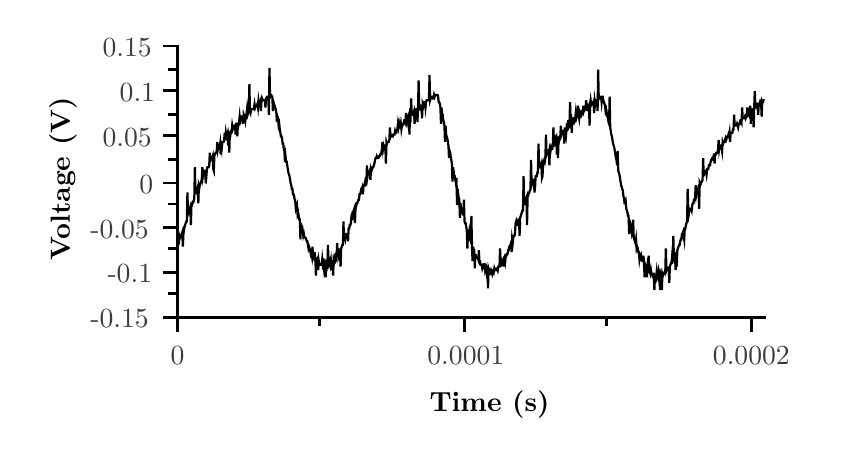
\begin{tikzpicture}{0pt}{0pt}{299pt}{150pt}
	\clip(0pt,150pt) -- (284.325pt,150pt) -- (284.325pt,7.36184pt) -- (0pt,7.36184pt) -- (0pt,150pt);
\begin{scope}
	\clip(54.2025pt,143.344pt) -- (266.258pt,143.344pt) -- (266.258pt,45.3987pt) -- (54.2025pt,45.3987pt) -- (54.2025pt,143.344pt);
	\color[gray]{0}
	\draw[line width=0.8pt, line join=miter, line cap=rect](54.4098pt,71.5173pt) -- (54.6171pt,72.1703pt) -- (54.8244pt,74.7821pt) -- (55.0317pt,74.1292pt) -- (55.2389pt,74.7821pt) -- (55.4462pt,74.7821pt) -- (55.6535pt,75.4351pt) -- (55.8608pt,76.0881pt) -- (56.0681pt,70.8644pt) -- (56.2754pt,75.4351pt) -- (56.4827pt,76.741pt) -- (56.69pt,78.047pt) -- (56.8972pt,78.6999pt) -- (57.1045pt,79.3529pt) -- (57.3118pt,80.0059pt) -- (57.5191pt,80.0059pt) -- (57.7264pt,90.4533pt) -- (57.9337pt,82.6177pt) -- (58.141pt,83.2707pt) -- (58.3483pt,84.5766pt) -- (58.5555pt,84.5766pt) -- (58.7628pt,85.2296pt) -- (58.9701pt,78.6999pt) -- (59.1774pt,85.8826pt) -- (59.3847pt,85.8826pt) -- (59.592pt,86.5355pt) -- (59.7993pt,87.1885pt) -- (60.0066pt,87.1885pt) -- (60.2138pt,88.4944pt) -- (60.4211pt,99.5948pt) -- (60.6284pt,89.8004pt) -- (60.8357pt,91.7593pt) -- (61.043pt,91.7593pt) -- (61.2503pt,91.7593pt) -- (61.4576pt,92.4122pt) -- (61.6649pt,86.5355pt) -- (61.8721pt,93.0652pt) -- (62.0794pt,92.4122pt) -- (62.2867pt,93.7182pt) -- (62.494pt,93.7182pt) -- (62.7013pt,94.3711pt) -- (62.9086pt,95.0241pt) -- (63.1159pt,99.5948pt) -- (63.3232pt,96.33pt) -- (63.5304pt,97.6359pt) -- (63.7377pt,97.6359pt) -- (63.945pt,98.2889pt) -- (64.1523pt,98.2889pt) -- (64.3596pt,93.7182pt) -- (64.5669pt,96.33pt) -- (64.7742pt,98.9419pt) -- (64.9815pt,99.5948pt) -- (65.1888pt,99.5948pt) -- (65.396pt,99.5948pt) -- (65.6033pt,100.248pt) -- (65.8106pt,104.819pt) -- (66.0179pt,102.207pt) -- (66.2252pt,102.86pt) -- (66.4325pt,102.86pt) -- (66.6398pt,102.86pt) -- (66.8471pt,103.513pt) -- (67.0543pt,98.9419pt) -- (67.2616pt,98.2889pt) -- (67.4689pt,104.166pt) -- (67.6762pt,104.166pt) -- (67.8835pt,104.819pt) -- (68.0908pt,104.819pt) -- (68.2981pt,104.819pt) -- (68.5054pt,108.736pt) -- (68.7126pt,106.125pt) -- (68.9199pt,107.43pt) -- (69.1272pt,107.43pt) -- (69.3345pt,106.777pt) -- (69.5418pt,108.083pt) -- (69.7491pt,104.166pt) -- (69.9564pt,108.736pt) -- (70.1637pt,106.777pt) -- (70.3709pt,108.736pt) -- (70.5782pt,108.736pt) -- (70.7855pt,108.736pt) -- (70.9928pt,109.389pt) -- (71.2001pt,112.001pt) -- (71.4074pt,109.389pt) -- (71.6147pt,112.001pt) -- (71.822pt,110.695pt) -- (72.0292pt,111.348pt) -- (72.2365pt,112.001pt) -- (72.4438pt,107.43pt) -- (72.6511pt,112.654pt) -- (72.8584pt,104.819pt) -- (73.0657pt,112.654pt) -- (73.273pt,111.348pt) -- (73.4803pt,112.654pt) -- (73.6876pt,112.654pt) -- (73.8948pt,114.613pt) -- (74.1021pt,113.307pt) -- (74.3094pt,113.96pt) -- (74.5167pt,113.96pt) -- (74.724pt,114.613pt) -- (74.9313pt,114.613pt) -- (75.1386pt,111.348pt) -- (75.3459pt,115.266pt) -- (75.5531pt,115.266pt) -- (75.7604pt,110.695pt) -- (75.9677pt,115.266pt) -- (76.175pt,115.266pt) -- (76.3823pt,115.919pt) -- (76.5896pt,117.878pt) -- (76.7969pt,115.919pt) -- (77.0042pt,116.572pt) -- (77.2114pt,116.572pt) -- (77.4187pt,117.878pt) -- (77.626pt,117.878pt) -- (77.8333pt,115.266pt) -- (78.0406pt,118.531pt) -- (78.2479pt,117.878pt) -- (78.4552pt,117.878pt) -- (78.6625pt,116.572pt) -- (78.8697pt,118.531pt) -- (79.077pt,118.531pt) -- (79.2843pt,120.49pt) -- (79.4916pt,118.531pt) -- (79.6989pt,119.184pt) -- (79.9062pt,119.837pt) -- (80.1135pt,129.631pt) -- (80.3208pt,119.837pt) -- (80.528pt,119.184pt) -- (80.7353pt,120.49pt) -- (80.9426pt,120.49pt) -- (81.1499pt,120.49pt) -- (81.3572pt,120.49pt) -- (81.5645pt,120.49pt) -- (81.7718pt,121.143pt) -- (81.9791pt,122.449pt) -- (82.1863pt,121.143pt) -- (82.3936pt,121.796pt) -- (82.6009pt,121.796pt) -- (82.8082pt,121.796pt) -- (83.0155pt,122.449pt) -- (83.2228pt,121.143pt) -- (83.4301pt,123.755pt) -- (83.6374pt,122.449pt) -- (83.8447pt,122.449pt) -- (84.0519pt,123.102pt) -- (84.2592pt,119.837pt) -- (84.4665pt,123.102pt) -- (84.6738pt,124.408pt) -- (84.8811pt,123.755pt) -- (85.0884pt,123.755pt) -- (85.2957pt,123.755pt) -- (85.503pt,123.755pt) -- (85.7102pt,123.755pt) -- (85.9175pt,121.143pt) -- (86.1248pt,124.408pt) -- (86.3321pt,124.408pt) -- (86.5394pt,125.061pt) -- (86.7467pt,125.061pt) -- (86.954pt,125.061pt) -- (87.1613pt,118.531pt) -- (87.3685pt,135.508pt) -- (87.5758pt,125.061pt) -- (87.7831pt,125.713pt) -- (87.9904pt,125.713pt) -- (88.1977pt,125.061pt) -- (88.405pt,125.061pt) -- (88.6123pt,119.837pt) -- (88.8196pt,123.102pt) -- (89.0268pt,122.449pt) -- (89.2341pt,121.796pt) -- (89.4414pt,121.143pt) -- (89.6487pt,120.49pt) -- (89.856pt,119.184pt) -- (90.0633pt,115.919pt) -- (90.2706pt,117.878pt) -- (90.4779pt,117.225pt) -- (90.6851pt,114.613pt) -- (90.8924pt,115.266pt) -- (91.0997pt,113.307pt) -- (91.307pt,112.001pt) -- (91.5143pt,110.695pt) -- (91.7216pt,110.695pt) -- (91.9289pt,110.042pt) -- (92.1362pt,108.083pt) -- (92.3435pt,108.083pt) -- (92.5507pt,106.125pt) -- (92.758pt,105.472pt) -- (92.9653pt,101.554pt) -- (93.1726pt,103.513pt) -- (93.3799pt,101.554pt) -- (93.5872pt,101.554pt) -- (93.7945pt,100.248pt) -- (94.0018pt,98.9419pt) -- (94.209pt,97.6359pt) -- (94.4163pt,96.983pt) -- (94.6236pt,96.33pt) -- (94.8309pt,95.0241pt) -- (95.0382pt,93.7182pt) -- (95.2455pt,93.0652pt) -- (95.4528pt,91.7593pt) -- (95.6601pt,91.7593pt) -- (95.8673pt,89.8004pt) -- (96.0746pt,89.8004pt) -- (96.2819pt,89.1474pt) -- (96.4892pt,87.8415pt) -- (96.6965pt,87.1885pt) -- (96.9038pt,84.5766pt) -- (97.1111pt,85.2296pt) -- (97.3184pt,85.8826pt) -- (97.5256pt,82.6177pt) -- (97.7329pt,83.2707pt) -- (97.9402pt,81.9648pt) -- (98.1475pt,80.6588pt) -- (98.3548pt,80.6588pt) -- (98.5621pt,73.4762pt) -- (98.7694pt,79.3529pt) -- (98.9767pt,78.047pt) -- (99.1839pt,78.047pt) -- (99.3912pt,76.741pt) -- (99.5985pt,74.7821pt) -- (99.8058pt,75.4351pt) -- (100.013pt,74.1292pt) -- (100.22pt,74.1292pt) -- (100.428pt,74.1292pt) -- (100.635pt,73.4762pt) -- (100.842pt,72.8232pt) -- (101.05pt,72.8232pt) -- (101.257pt,71.5173pt) -- (101.464pt,70.2114pt) -- (101.671pt,70.8644pt) -- (101.879pt,70.2114pt) -- (102.086pt,69.5584pt) -- (102.293pt,68.2525pt) -- (102.501pt,68.9055pt) -- (102.708pt,67.5995pt) -- (102.915pt,70.8644pt) -- (103.122pt,66.9466pt) -- (103.33pt,67.5995pt) -- (103.537pt,66.9466pt) -- (103.744pt,68.9055pt) -- (103.952pt,66.2936pt) -- (104.159pt,60.4169pt) -- (104.366pt,66.9466pt) -- (104.573pt,65.6406pt) -- (104.781pt,66.2936pt) -- (104.988pt,62.3758pt) -- (105.195pt,65.6406pt) -- (105.403pt,64.3347pt) -- (105.61pt,64.3347pt) -- (105.817pt,64.3347pt) -- (106.024pt,64.3347pt) -- (106.232pt,64.3347pt) -- (106.439pt,66.2936pt) -- (106.646pt,64.3347pt) -- (106.854pt,64.9877pt) -- (107.061pt,63.0288pt) -- (107.268pt,64.9877pt) -- (107.475pt,64.3347pt) -- (107.683pt,59.7639pt) -- (107.89pt,64.3347pt) -- (108.097pt,63.6817pt) -- (108.305pt,64.3347pt) -- (108.512pt,71.5173pt) -- (108.719pt,64.3347pt) -- (108.926pt,64.9877pt) -- (109.134pt,65.6406pt) -- (109.341pt,64.3347pt) -- (109.548pt,65.6406pt) -- (109.756pt,62.3758pt) -- (109.963pt,65.6406pt) -- (110.17pt,65.6406pt) -- (110.377pt,60.4169pt) -- (110.585pt,66.2936pt) -- (110.792pt,65.6406pt) -- (110.999pt,66.9466pt) -- (111.207pt,66.2936pt) -- (111.414pt,67.5995pt) -- (111.621pt,66.9466pt) -- (111.829pt,72.1703pt) -- (112.036pt,68.2525pt) -- (112.243pt,68.9055pt) -- (112.45pt,68.9055pt) -- (112.658pt,65.6406pt) -- (112.865pt,70.2114pt) -- (113.072pt,63.6817pt) -- (113.28pt,70.2114pt) -- (113.487pt,70.8644pt) -- (113.694pt,71.5173pt) -- (113.901pt,71.5173pt) -- (114.109pt,80.0059pt) -- (114.316pt,72.8232pt) -- (114.523pt,74.1292pt) -- (114.731pt,73.4762pt) -- (114.938pt,75.4351pt) -- (115.145pt,75.4351pt) -- (115.352pt,75.4351pt) -- (115.56pt,75.4351pt) -- (115.767pt,72.8232pt) -- (115.974pt,77.394pt) -- (116.182pt,77.394pt) -- (116.389pt,78.6999pt) -- (116.596pt,78.6999pt) -- (116.803pt,79.3529pt) -- (117.011pt,81.9648pt) -- (117.218pt,82.6177pt) -- (117.425pt,81.9648pt) -- (117.633pt,83.2707pt) -- (117.84pt,83.9237pt) -- (118.047pt,84.5766pt) -- (118.254pt,79.3529pt) -- (118.462pt,84.5766pt) -- (118.669pt,85.2296pt) -- (118.876pt,86.5355pt) -- (119.084pt,86.5355pt) -- (119.291pt,87.1885pt) -- (119.498pt,87.8415pt) -- (119.705pt,87.8415pt) -- (119.913pt,89.8004pt) -- (120.12pt,89.8004pt) -- (120.327pt,90.4533pt) -- (120.535pt,91.7593pt) -- (120.742pt,91.7593pt) -- (120.949pt,92.4122pt) -- (121.156pt,89.8004pt) -- (121.364pt,93.0652pt) -- (121.571pt,93.0652pt) -- (121.778pt,93.0652pt) -- (121.986pt,94.3711pt) -- (122.193pt,93.7182pt) -- (122.4pt,94.3711pt) -- (122.607pt,100.248pt) -- (122.815pt,96.33pt) -- (123.022pt,97.6359pt) -- (123.229pt,97.6359pt) -- (123.437pt,97.6359pt) -- (123.644pt,98.2889pt) -- (123.851pt,95.0241pt) -- (124.058pt,98.9419pt) -- (124.266pt,98.2889pt) -- (124.473pt,98.9419pt) -- (124.68pt,99.5948pt) -- (124.888pt,99.5948pt) -- (125.095pt,100.248pt) -- (125.302pt,100.901pt) -- (125.509pt,102.207pt) -- (125.717pt,102.86pt) -- (125.924pt,102.86pt) -- (126.131pt,103.513pt) -- (126.339pt,102.86pt) -- (126.546pt,102.86pt) -- (126.753pt,102.86pt) -- (126.961pt,103.513pt) -- (127.168pt,103.513pt) -- (127.375pt,104.166pt) -- (127.582pt,104.166pt) -- (127.79pt,104.819pt) -- (127.997pt,106.125pt) -- (128.204pt,108.736pt) -- (128.412pt,106.125pt) -- (128.619pt,107.43pt) -- (128.826pt,106.777pt) -- (129.033pt,107.43pt) -- (129.241pt,107.43pt) -- (129.448pt,100.901pt) -- (129.655pt,108.736pt) -- (129.863pt,108.083pt) -- (130.07pt,108.736pt) -- (130.277pt,108.736pt) -- (130.484pt,108.736pt) -- (130.692pt,109.389pt) -- (130.899pt,113.96pt) -- (131.106pt,110.695pt) -- (131.314pt,111.348pt) -- (131.521pt,111.348pt) -- (131.728pt,110.695pt) -- (131.935pt,110.695pt) -- (132.143pt,111.348pt) -- (132.35pt,111.348pt) -- (132.557pt,111.348pt) -- (132.765pt,112.654pt) -- (132.972pt,112.001pt) -- (133.179pt,112.001pt) -- (133.386pt,112.654pt) -- (133.594pt,113.307pt) -- (133.801pt,115.266pt) -- (134.008pt,113.96pt) -- (134.216pt,115.266pt) -- (134.423pt,113.96pt) -- (134.63pt,113.96pt) -- (134.837pt,115.266pt) -- (135.045pt,113.307pt) -- (135.252pt,114.613pt) -- (135.459pt,114.613pt) -- (135.667pt,115.266pt) -- (135.874pt,115.266pt) -- (136.081pt,116.572pt) -- (136.288pt,116.572pt) -- (136.496pt,115.919pt) -- (136.703pt,119.184pt) -- (136.91pt,117.225pt) -- (137.118pt,115.919pt) -- (137.325pt,117.225pt) -- (137.532pt,117.878pt) -- (137.739pt,118.531pt) -- (137.947pt,111.348pt) -- (138.154pt,118.531pt) -- (138.361pt,117.878pt) -- (138.569pt,124.408pt) -- (138.776pt,118.531pt) -- (138.983pt,118.531pt) -- (139.19pt,118.531pt) -- (139.398pt,119.184pt) -- (139.605pt,119.837pt) -- (139.812pt,115.266pt) -- (140.02pt,119.837pt) -- (140.227pt,119.837pt) -- (140.434pt,120.49pt) -- (140.642pt,120.49pt) -- (140.849pt,115.919pt) -- (141.056pt,121.143pt) -- (141.263pt,130.937pt) -- (141.471pt,121.143pt) -- (141.678pt,121.796pt) -- (141.885pt,121.143pt) -- (142.093pt,121.796pt) -- (142.3pt,121.796pt) -- (142.507pt,117.225pt) -- (142.714pt,122.449pt) -- (142.922pt,121.796pt) -- (143.129pt,123.102pt) -- (143.336pt,123.102pt) -- (143.544pt,123.102pt) -- (143.751pt,121.143pt) -- (143.958pt,123.102pt) -- (144.165pt,123.755pt) -- (144.373pt,123.755pt) -- (144.58pt,123.755pt) -- (144.787pt,123.755pt) -- (144.995pt,123.755pt) -- (145.202pt,132.896pt) -- (145.409pt,123.755pt) -- (145.616pt,124.408pt) -- (145.824pt,125.061pt) -- (146.031pt,125.061pt) -- (146.238pt,125.061pt) -- (146.446pt,124.408pt) -- (146.653pt,124.408pt) -- (146.86pt,125.713pt) -- (147.067pt,125.061pt) -- (147.275pt,125.713pt) -- (147.482pt,125.713pt) -- (147.689pt,125.713pt) -- (147.897pt,125.713pt) -- (148.104pt,125.713pt) -- (148.311pt,125.061pt) -- (148.518pt,123.102pt) -- (148.726pt,123.102pt) -- (148.933pt,122.449pt) -- (149.14pt,121.143pt) -- (149.348pt,115.266pt) -- (149.555pt,121.143pt) -- (149.762pt,118.531pt) -- (149.969pt,118.531pt) -- (150.177pt,116.572pt) -- (150.384pt,115.919pt) -- (150.591pt,114.613pt) -- (150.799pt,108.736pt) -- (151.006pt,114.613pt) -- (151.213pt,111.348pt) -- (151.42pt,110.695pt) -- (151.628pt,110.042pt) -- (151.835pt,108.736pt) -- (152.042pt,107.43pt) -- (152.25pt,102.86pt) -- (152.457pt,105.472pt) -- (152.664pt,104.819pt) -- (152.871pt,103.513pt) -- (153.079pt,102.207pt) -- (153.286pt,100.901pt) -- (153.493pt,94.3711pt) -- (153.701pt,99.5948pt) -- (153.908pt,98.2889pt) -- (154.115pt,96.33pt) -- (154.322pt,96.33pt) -- (154.53pt,95.0241pt) -- (154.737pt,93.7182pt) -- (154.944pt,95.6771pt) -- (155.152pt,85.8826pt) -- (155.359pt,91.7593pt) -- (155.566pt,89.8004pt) -- (155.774pt,88.4944pt) -- (155.981pt,87.8415pt) -- (156.188pt,81.3118pt) -- (156.395pt,86.5355pt) -- (156.603pt,84.5766pt) -- (156.81pt,84.5766pt) -- (157.017pt,83.2707pt) -- (157.225pt,82.6177pt) -- (157.432pt,82.6177pt) -- (157.639pt,87.8415pt) -- (157.846pt,80.0059pt) -- (158.054pt,79.3529pt) -- (158.261pt,79.3529pt) -- (158.468pt,78.047pt) -- (158.676pt,76.741pt) -- (158.883pt,70.2114pt) -- (159.09pt,75.4351pt) -- (159.297pt,74.7821pt) -- (159.505pt,76.0881pt) -- (159.712pt,73.4762pt) -- (159.919pt,73.4762pt) -- (160.127pt,72.8232pt) -- (160.334pt,81.9648pt) -- (160.541pt,71.5173pt) -- (160.748pt,65.6406pt) -- (160.956pt,70.8644pt) -- (161.163pt,69.5584pt) -- (161.37pt,69.5584pt) -- (161.578pt,63.0288pt) -- (161.785pt,68.2525pt) -- (161.992pt,66.9466pt) -- (162.199pt,66.9466pt) -- (162.407pt,66.9466pt) -- (162.614pt,66.9466pt) -- (162.821pt,66.2936pt) -- (163.029pt,69.5584pt) -- (163.236pt,65.6406pt) -- (163.443pt,65.6406pt) -- (163.65pt,64.3347pt) -- (163.858pt,64.3347pt) -- (164.065pt,64.3347pt) -- (164.272pt,63.0288pt) -- (164.48pt,63.6817pt) -- (164.687pt,63.0288pt) -- (164.894pt,63.0288pt) -- (165.101pt,64.9877pt) -- (165.309pt,62.3758pt) -- (165.516pt,63.0288pt) -- (165.723pt,61.7228pt) -- (165.931pt,63.0288pt) -- (166.138pt,62.3758pt) -- (166.345pt,55.8461pt) -- (166.552pt,63.0288pt) -- (166.76pt,62.3758pt) -- (166.967pt,62.3758pt) -- (167.174pt,61.7228pt) -- (167.382pt,62.3758pt) -- (167.589pt,61.7228pt) -- (167.796pt,61.0699pt) -- (168.003pt,62.3758pt) -- (168.211pt,62.3758pt) -- (168.418pt,61.7228pt) -- (168.625pt,63.0288pt) -- (168.833pt,62.3758pt) -- (169.04pt,62.3758pt) -- (169.247pt,62.3758pt) -- (169.455pt,63.0288pt) -- (169.662pt,63.0288pt) -- (169.869pt,62.3758pt) -- (170.076pt,63.6817pt) -- (170.284pt,63.6817pt) -- (170.491pt,63.6817pt) -- (170.698pt,70.2114pt) -- (170.906pt,63.6817pt) -- (171.113pt,64.9877pt) -- (171.32pt,65.6406pt) -- (171.527pt,64.9877pt) -- (171.735pt,65.6406pt) -- (171.942pt,63.6817pt) -- (172.149pt,66.2936pt) -- (172.357pt,66.9466pt) -- (172.564pt,65.6406pt) -- (172.771pt,67.5995pt) -- (172.978pt,67.5995pt) -- (173.186pt,68.2525pt) -- (173.393pt,68.2525pt) -- (173.6pt,69.5584pt) -- (173.808pt,69.5584pt) -- (174.015pt,70.8644pt) -- (174.222pt,70.8644pt) -- (174.429pt,71.5173pt) -- (174.637pt,72.1703pt) -- (174.844pt,68.9055pt) -- (175.051pt,73.4762pt) -- (175.259pt,72.1703pt) -- (175.466pt,74.1292pt) -- (175.673pt,74.7821pt) -- (175.88pt,74.7821pt) -- (176.088pt,75.4351pt) -- (176.295pt,79.3529pt) -- (176.502pt,80.0059pt) -- (176.71pt,78.6999pt) -- (176.917pt,78.6999pt) -- (177.124pt,79.3529pt) -- (177.331pt,80.6588pt) -- (177.539pt,80.6588pt) -- (177.746pt,74.7821pt) -- (177.953pt,81.3118pt) -- (178.161pt,81.9648pt) -- (178.368pt,82.6177pt) -- (178.575pt,83.2707pt) -- (178.782pt,83.9237pt) -- (178.99pt,83.9237pt) -- (179.197pt,96.33pt) -- (179.404pt,85.8826pt) -- (179.612pt,87.1885pt) -- (179.819pt,87.1885pt) -- (180.026pt,87.8415pt) -- (180.233pt,88.4944pt) -- (180.441pt,78.6999pt) -- (180.648pt,89.1474pt) -- (180.855pt,89.1474pt) -- (181.063pt,90.4533pt) -- (181.27pt,90.4533pt) -- (181.477pt,91.1063pt) -- (181.684pt,91.7593pt) -- (181.892pt,102.207pt) -- (182.099pt,93.0652pt) -- (182.306pt,93.7182pt) -- (182.514pt,94.3711pt) -- (182.721pt,95.0241pt) -- (182.928pt,95.0241pt) -- (183.135pt,90.4533pt) -- (183.343pt,92.4122pt) -- (183.55pt,96.33pt) -- (183.757pt,96.33pt) -- (183.965pt,96.33pt) -- (184.172pt,97.6359pt) -- (184.379pt,97.6359pt) -- (184.587pt,108.083pt) -- (184.794pt,99.5948pt) -- (185.001pt,99.5948pt) -- (185.208pt,100.248pt) -- (185.416pt,100.248pt) -- (185.623pt,100.901pt) -- (185.83pt,95.6771pt) -- (186.038pt,96.33pt) -- (186.245pt,100.901pt) -- (186.452pt,101.554pt) -- (186.659pt,102.207pt) -- (186.867pt,101.554pt) -- (187.074pt,102.86pt) -- (187.281pt,111.348pt) -- (187.489pt,104.166pt) -- (187.696pt,104.819pt) -- (187.903pt,104.819pt) -- (188.11pt,104.819pt) -- (188.318pt,105.472pt) -- (188.525pt,100.248pt) -- (188.732pt,106.125pt) -- (188.94pt,105.472pt) -- (189.147pt,106.777pt) -- (189.354pt,106.125pt) -- (189.561pt,106.125pt) -- (189.769pt,107.43pt) -- (189.976pt,113.96pt) -- (190.183pt,107.43pt) -- (190.391pt,111.348pt) -- (190.598pt,108.736pt) -- (190.805pt,109.389pt) -- (191.012pt,110.042pt) -- (191.22pt,104.166pt) -- (191.427pt,110.042pt) -- (191.634pt,102.86pt) -- (191.842pt,110.695pt) -- (192.049pt,109.389pt) -- (192.256pt,110.695pt) -- (192.463pt,110.695pt) -- (192.671pt,114.613pt) -- (192.878pt,111.348pt) -- (193.085pt,112.001pt) -- (193.293pt,112.001pt) -- (193.5pt,112.654pt) -- (193.707pt,112.654pt) -- (193.914pt,108.083pt) -- (194.122pt,113.96pt) -- (194.329pt,112.654pt) -- (194.536pt,111.348pt) -- (194.744pt,113.96pt) -- (194.951pt,113.307pt) -- (195.158pt,113.96pt) -- (195.365pt,116.572pt) -- (195.573pt,114.613pt) -- (195.78pt,115.266pt) -- (195.987pt,123.102pt) -- (196.195pt,115.919pt) -- (196.402pt,116.572pt) -- (196.609pt,112.001pt) -- (196.816pt,116.572pt) -- (197.024pt,115.919pt) -- (197.231pt,116.572pt) -- (197.438pt,115.919pt) -- (197.646pt,116.572pt) -- (197.853pt,117.225pt) -- (198.06pt,119.184pt) -- (198.268pt,117.225pt) -- (198.475pt,117.878pt) -- (198.682pt,117.878pt) -- (198.889pt,121.796pt) -- (199.097pt,118.531pt) -- (199.304pt,117.225pt) -- (199.511pt,119.184pt) -- (199.719pt,118.531pt) -- (199.926pt,119.184pt) -- (200.133pt,118.531pt) -- (200.34pt,119.184pt) -- (200.548pt,119.184pt) -- (200.755pt,121.796pt) -- (200.962pt,119.837pt) -- (201.17pt,120.49pt) -- (201.377pt,120.49pt) -- (201.584pt,120.49pt) -- (201.791pt,123.755pt) -- (201.999pt,119.837pt) -- (202.206pt,121.796pt) -- (202.413pt,121.143pt) -- (202.621pt,121.143pt) -- (202.828pt,121.796pt) -- (203.035pt,114.613pt) -- (203.242pt,121.796pt) -- (203.45pt,123.755pt) -- (203.657pt,122.449pt) -- (203.864pt,123.102pt) -- (204.072pt,123.102pt) -- (204.279pt,122.449pt) -- (204.486pt,123.102pt) -- (204.693pt,119.184pt) -- (204.901pt,123.755pt) -- (205.108pt,122.449pt) -- (205.315pt,123.755pt) -- (205.523pt,123.755pt) -- (205.73pt,123.755pt) -- (205.937pt,119.837pt) -- (206.144pt,134.855pt) -- (206.352pt,124.408pt) -- (206.559pt,125.061pt) -- (206.766pt,125.061pt) -- (206.974pt,125.061pt) -- (207.181pt,125.061pt) -- (207.388pt,123.102pt) -- (207.595pt,125.061pt) -- (207.803pt,125.061pt) -- (208.01pt,123.755pt) -- (208.217pt,123.102pt) -- (208.425pt,122.449pt) -- (208.632pt,121.796pt) -- (208.839pt,119.837pt) -- (209.046pt,120.49pt) -- (209.254pt,119.184pt) -- (209.461pt,117.878pt) -- (209.668pt,117.878pt) -- (209.876pt,115.919pt) -- (210.083pt,115.266pt) -- (210.29pt,125.061pt) -- (210.497pt,113.96pt) -- (210.705pt,112.654pt) -- (210.912pt,111.348pt) -- (211.119pt,110.695pt) -- (211.327pt,109.389pt) -- (211.534pt,108.083pt) -- (211.741pt,107.43pt) -- (211.948pt,106.777pt) -- (212.156pt,105.472pt) -- (212.363pt,104.166pt) -- (212.57pt,102.86pt) -- (212.778pt,102.207pt) -- (212.985pt,100.248pt) -- (213.192pt,105.472pt) -- (213.4pt,98.2889pt) -- (213.607pt,97.6359pt) -- (213.814pt,96.983pt) -- (214.021pt,95.6771pt) -- (214.229pt,94.3711pt) -- (214.436pt,93.0652pt) -- (214.643pt,92.4122pt) -- (214.851pt,91.7593pt) -- (215.058pt,91.1063pt) -- (215.265pt,89.1474pt) -- (215.472pt,88.4944pt) -- (215.68pt,86.5355pt) -- (215.887pt,86.5355pt) -- (216.094pt,87.1885pt) -- (216.302pt,84.5766pt) -- (216.509pt,83.9237pt) -- (216.716pt,83.2707pt) -- (216.923pt,81.9648pt) -- (217.131pt,81.9648pt) -- (217.338pt,75.4351pt) -- (217.545pt,80.0059pt) -- (217.753pt,79.3529pt) -- (217.96pt,78.047pt) -- (218.167pt,77.394pt) -- (218.374pt,75.4351pt) -- (218.582pt,76.0881pt) -- (218.789pt,80.6588pt) -- (218.996pt,74.1292pt) -- (219.204pt,73.4762pt) -- (219.411pt,72.8232pt) -- (219.618pt,72.1703pt) -- (219.825pt,73.4762pt) -- (220.033pt,70.2114pt) -- (220.24pt,70.8644pt) -- (220.447pt,70.2114pt) -- (220.655pt,68.9055pt) -- (220.862pt,68.9055pt) -- (221.069pt,66.2936pt) -- (221.276pt,67.5995pt) -- (221.484pt,66.9466pt) -- (221.691pt,67.5995pt) -- (221.898pt,66.2936pt) -- (222.106pt,65.6406pt) -- (222.313pt,65.6406pt) -- (222.52pt,67.5995pt) -- (222.727pt,64.3347pt) -- (222.935pt,59.7639pt) -- (223.142pt,64.3347pt) -- (223.349pt,63.6817pt) -- (223.557pt,63.0288pt) -- (223.764pt,59.7639pt) -- (223.971pt,63.0288pt) -- (224.178pt,61.7228pt) -- (224.386pt,67.5995pt) -- (224.593pt,61.7228pt) -- (224.8pt,61.7228pt) -- (225.008pt,61.0699pt) -- (225.215pt,62.3758pt) -- (225.422pt,61.0699pt) -- (225.629pt,61.0699pt) -- (225.837pt,60.4169pt) -- (226.044pt,61.0699pt) -- (226.251pt,61.0699pt) -- (226.459pt,55.1932pt) -- (226.666pt,60.4169pt) -- (226.873pt,60.4169pt) -- (227.081pt,59.7639pt) -- (227.288pt,61.7228pt) -- (227.495pt,59.7639pt) -- (227.702pt,60.4169pt) -- (227.91pt,61.7228pt) -- (228.117pt,59.7639pt) -- (228.324pt,61.0699pt) -- (228.532pt,55.1932pt) -- (228.739pt,61.0699pt) -- (228.946pt,60.4169pt) -- (229.153pt,55.1932pt) -- (229.361pt,61.0699pt) -- (229.568pt,60.4169pt) -- (229.775pt,61.0699pt) -- (229.983pt,61.0699pt) -- (230.19pt,61.7228pt) -- (230.397pt,61.7228pt) -- (230.604pt,70.2114pt) -- (230.812pt,62.3758pt) -- (231.019pt,63.0288pt) -- (231.226pt,62.3758pt) -- (231.434pt,62.3758pt) -- (231.641pt,63.6817pt) -- (231.848pt,57.805pt) -- (232.055pt,63.6817pt) -- (232.263pt,64.3347pt) -- (232.47pt,64.9877pt) -- (232.677pt,64.9877pt) -- (232.885pt,67.5995pt) -- (233.092pt,66.2936pt) -- (233.299pt,74.7821pt) -- (233.506pt,66.9466pt) -- (233.714pt,67.5995pt) -- (233.921pt,67.5995pt) -- (234.128pt,62.3758pt) -- (234.336pt,68.9055pt) -- (234.543pt,63.6817pt) -- (234.75pt,69.5584pt) -- (234.957pt,70.2114pt) -- (235.165pt,70.8644pt) -- (235.372pt,71.5173pt) -- (235.579pt,71.5173pt) -- (235.787pt,72.8232pt) -- (235.994pt,73.4762pt) -- (236.201pt,73.4762pt) -- (236.408pt,75.4351pt) -- (236.616pt,75.4351pt) -- (236.823pt,76.0881pt) -- (237.03pt,74.7821pt) -- (237.238pt,73.4762pt) -- (237.445pt,77.394pt) -- (237.652pt,77.394pt) -- (237.859pt,78.6999pt) -- (238.067pt,79.3529pt) -- (238.274pt,80.0059pt) -- (238.481pt,91.7593pt) -- (238.689pt,84.5766pt) -- (238.896pt,82.6177pt) -- (239.103pt,83.9237pt) -- (239.31pt,84.5766pt) -- (239.518pt,84.5766pt) -- (239.725pt,84.5766pt) -- (239.932pt,83.9237pt) -- (240.14pt,85.8826pt) -- (240.347pt,86.5355pt) -- (240.554pt,86.5355pt) -- (240.761pt,87.8415pt) -- (240.969pt,87.8415pt) -- (241.176pt,88.4944pt) -- (241.383pt,93.0652pt) -- (241.591pt,89.8004pt) -- (241.798pt,91.1063pt) -- (242.005pt,91.7593pt) -- (242.213pt,91.7593pt) -- (242.42pt,92.4122pt) -- (242.627pt,84.5766pt) -- (242.834pt,93.7182pt) -- (243.042pt,93.0652pt) -- (243.249pt,93.7182pt) -- (243.456pt,94.3711pt) -- (243.664pt,94.3711pt) -- (243.871pt,95.0241pt) -- (244.078pt,102.86pt) -- (244.285pt,96.33pt) -- (244.493pt,97.6359pt) -- (244.7pt,97.6359pt) -- (244.907pt,98.2889pt) -- (245.115pt,98.2889pt) -- (245.322pt,96.983pt) -- (245.529pt,98.9419pt) -- (245.736pt,98.9419pt) -- (245.944pt,98.9419pt) -- (246.151pt,100.248pt) -- (246.358pt,100.248pt) -- (246.566pt,100.248pt) -- (246.773pt,101.554pt) -- (246.98pt,102.207pt) -- (247.187pt,102.207pt) -- (247.395pt,102.86pt) -- (247.602pt,102.86pt) -- (247.809pt,103.513pt) -- (248.017pt,102.86pt) -- (248.224pt,100.901pt) -- (248.431pt,104.166pt) -- (248.638pt,104.166pt) -- (248.846pt,104.819pt) -- (249.053pt,104.819pt) -- (249.26pt,104.819pt) -- (249.468pt,106.125pt) -- (249.675pt,109.389pt) -- (249.882pt,106.125pt) -- (250.089pt,107.43pt) -- (250.297pt,107.43pt) -- (250.504pt,107.43pt) -- (250.711pt,106.777pt) -- (250.919pt,105.472pt) -- (251.126pt,108.736pt) -- (251.333pt,108.083pt) -- (251.54pt,108.736pt) -- (251.748pt,108.736pt) -- (251.955pt,109.389pt) -- (252.162pt,110.042pt) -- (252.37pt,109.389pt) -- (252.577pt,110.042pt) -- (252.784pt,110.695pt) -- (252.991pt,110.695pt) -- (253.199pt,111.348pt) -- (253.406pt,110.695pt) -- (253.613pt,112.001pt) -- (253.821pt,108.736pt) -- (254.028pt,112.001pt) -- (254.235pt,112.001pt) -- (254.442pt,112.001pt) -- (254.65pt,112.001pt) -- (254.857pt,113.307pt) -- (255.064pt,113.307pt) -- (255.272pt,118.531pt) -- (255.479pt,114.613pt) -- (255.686pt,114.613pt) -- (255.894pt,114.613pt) -- (256.101pt,114.613pt) -- (256.308pt,115.266pt) -- (256.515pt,114.613pt) -- (256.723pt,113.96pt) -- (256.93pt,115.266pt) -- (257.137pt,115.266pt) -- (257.345pt,115.266pt) -- (257.552pt,116.572pt) -- (257.759pt,116.572pt) -- (257.966pt,115.919pt) -- (258.174pt,121.143pt) -- (258.381pt,117.225pt) -- (258.588pt,117.225pt) -- (258.796pt,117.225pt) -- (259.003pt,117.225pt) -- (259.21pt,117.878pt) -- (259.417pt,117.225pt) -- (259.625pt,117.878pt) -- (259.832pt,117.878pt) -- (260.039pt,121.143pt) -- (260.247pt,119.184pt) -- (260.454pt,119.184pt) -- (260.661pt,118.531pt) -- (260.868pt,119.184pt) -- (261.076pt,121.796pt) -- (261.283pt,115.266pt) -- (261.49pt,119.837pt) -- (261.698pt,120.49pt) -- (261.905pt,120.49pt) -- (262.112pt,120.49pt) -- (262.319pt,113.96pt) -- (262.527pt,121.143pt) -- (262.734pt,127.019pt) -- (262.941pt,121.796pt) -- (263.149pt,121.143pt) -- (263.356pt,121.143pt) -- (263.563pt,121.796pt) -- (263.77pt,121.143pt) -- (263.978pt,118.531pt) -- (264.185pt,122.449pt) -- (264.392pt,122.449pt) -- (264.6pt,123.102pt) -- (264.807pt,122.449pt) -- (265.014pt,123.102pt) -- (265.221pt,117.878pt) -- (265.429pt,123.102pt) -- (265.636pt,123.102pt) -- (265.843pt,123.755pt) -- (266.051pt,123.755pt) -- (266.258pt,123.755pt);
\end{scope}
\begin{scope}
	\color[gray]{0}
	\pgftext[center, base, at={\pgfpoint{15.2147pt}{95.3146pt}},rotate=90]{\textbf{Voltage (V)}}
	\color[gray]{0.235294}
	\pgftext[center, base, at={\pgfpoint{33.2154pt}{41.595pt}}]{-0.15}
	\pgftext[center, base, at={\pgfpoint{36.9076pt}{57.7607pt}}]{-0.1}
	\pgftext[center, base, at={\pgfpoint{33.2154pt}{73.9263pt}}]{-0.05}
	\pgftext[center, base, at={\pgfpoint{42.9029pt}{90.092pt}}]{0}
	\pgftext[center, base, at={\pgfpoint{35.9567pt}{107.209pt}}]{0.05}
	\pgftext[center, base, at={\pgfpoint{39.649pt}{123.374pt}}]{0.1}
	\pgftext[center, base, at={\pgfpoint{35.9567pt}{139.54pt}}]{0.15}
	\color[gray]{0}
	\draw[line width=1pt, line join=bevel, line cap=rect](54.2025pt,53.957pt) -- (51.3497pt,53.957pt);
	\draw[line width=1pt, line join=bevel, line cap=rect](54.2025pt,70.1226pt) -- (51.3497pt,70.1226pt);
	\draw[line width=1pt, line join=bevel, line cap=rect](54.2025pt,86.2883pt) -- (51.3497pt,86.2883pt);
	\draw[line width=1pt, line join=bevel, line cap=rect](54.2025pt,102.454pt) -- (51.3497pt,102.454pt);
	\draw[line width=1pt, line join=bevel, line cap=rect](54.2025pt,118.62pt) -- (51.3497pt,118.62pt);
	\draw[line width=1pt, line join=bevel, line cap=rect](54.2025pt,134.785pt) -- (51.3497pt,134.785pt);
	\draw[line width=1pt, line join=bevel, line cap=rect](54.2025pt,45.3987pt) -- (49.4479pt,45.3987pt);
	\draw[line width=1pt, line join=bevel, line cap=rect](54.2025pt,61.5643pt) -- (49.4479pt,61.5643pt);
	\draw[line width=1pt, line join=bevel, line cap=rect](54.2025pt,77.73pt) -- (49.4479pt,77.73pt);
	\draw[line width=1pt, line join=bevel, line cap=rect](54.2025pt,93.8957pt) -- (49.4479pt,93.8957pt);
	\draw[line width=1pt, line join=bevel, line cap=rect](54.2025pt,111.012pt) -- (49.4479pt,111.012pt);
	\draw[line width=1pt, line join=bevel, line cap=rect](54.2025pt,127.178pt) -- (49.4479pt,127.178pt);
	\draw[line width=1pt, line join=bevel, line cap=rect](54.2025pt,143.344pt) -- (49.4479pt,143.344pt);
	\draw[line width=1pt, line join=bevel, line cap=rect](54.2025pt,143.344pt) -- (54.2025pt,45.3987pt);
	\pgftext[center, base, at={\pgfpoint{166.887pt}{11.1655pt}}]{\textbf{Time (s)}}
	\color[gray]{0.235294}
	\pgftext[center, base, at={\pgfpoint{54.1951pt}{28.2821pt}}]{0}
	\pgftext[center, base, at={\pgfpoint{158.328pt}{28.2821pt}}]{0.0001}
	\pgftext[center, base, at={\pgfpoint{261.503pt}{28.2821pt}}]{0.0002}
	\color[gray]{0}
	\draw[line width=1pt, line join=bevel, line cap=rect](105.552pt,45.3987pt) -- (105.552pt,42.5459pt);
	\draw[line width=1pt, line join=bevel, line cap=rect](209.203pt,45.3987pt) -- (209.203pt,42.5459pt);
	\draw[line width=1pt, line join=bevel, line cap=rect](54.2025pt,45.3987pt) -- (54.2025pt,40.6441pt);
	\draw[line width=1pt, line join=bevel, line cap=rect](157.853pt,45.3987pt) -- (157.853pt,40.6441pt);
	\draw[line width=1pt, line join=bevel, line cap=rect](261.503pt,45.3987pt) -- (261.503pt,40.6441pt);
	\draw[line width=1pt, line join=bevel, line cap=rect](54.2025pt,45.3987pt) -- (266.258pt,45.3987pt);
\end{scope}
\end{tikzpicture}

		\caption{New signal produced when the two 7555 chips are used in the circuit and combined by the mixer.}
		\label{fig:7555}
\end{figure}

\subsection{Mixer - SA612A}
\label{sec:SA612A-mixer}
The mixer chip is used to calculate the difference in frequency between the input signals and output this difference as a new signal. This allows a small influence to the circuit to cause a big difference in the signal by comparing two high frequency inputs so that the relative difference is large. The chip that is used is the SA612A IC which is a double-balanced mixer and oscillator\cite{SA612A}. The pin configuration and internal block configuration is shown in appendix~\ref{app:SA612A}. This particular mixer chip subtracts the lower frequency signal from the higher one to give a simple difference relation.

The chip is tested using a pair of TG315 signal generators to provide a known input frequency that can be used to examine the performance of the mixer chip. It is found, when using this set-up, that though the output signal is the difference between the inputs, as expected, the signal is not perfectly clean, and there is a considerable amount of high frequency noise left. This produces a unpleasant rough high pitched addition to the sound. This is required to be removed in order that the instrument be acceptable to listen to. These unwanted parts of the signal shall be removed using a low pass filter.

\subsection{Low Pass Filter}
\label{sec:lowpass}
A low pass filter is a circuit whose output depends on the frequency of the input. The circuit has a cut off frequency, above which the amplitude of the signal is severely attenuated. This cut-off can be chosen depending on the components used. This allows the high frequency noise to be removed whilst leaving the important signal largely unaffected.

The low pass filter is composed of a resistor and a capacitor to ground, as shown in figure~\ref{fig:low_pass}. The capacitor acts as an open circuit at low frequency signals, so these parts are not affected, but acts as a short circuit at high frequencies, so these pass to ground and hence are removed from signal. To satisfactorily remove the noise, two low pass filters are placed in series with a $\times 1$ buffer amplifier between them. This produces a sharper cut-off so that less of the important signal is lost. The buffer amplifier is added to ensure the two filters are isolated from each other. It is formed of an operational-amplifier (op-amp) with the output fed back into the inverting input. The op-amp used is the LT081 operational amplifier, described in appendix~\ref{app:lt081}.

\begin{figure}[htbp]
	\begin{center}
		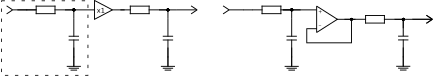
\includegraphics[width=\textwidth]{report_img/buffer_amp}
		\caption{The low pass filter is an extremely simple circuit to remove unwanted high frequency noise. The circuit on the left shows the principle of having two low pass filters separated by a $\times 1$ buffer amplifier, with the single low pass filter highlighted. The second circuit shows the implementation of the op-amp bases buffer.}
		\label{fig:low_pass}
	\end{center}
\end{figure}

The approximate frequency of the cut-off of the low pass filter is given by the equation
\begin{equation}
	f_c = \frac{1}{2\pi RC},
\end{equation}
where $R$ is the resistor and $C$ is the capacitor in the previous circuit. A cut-off of around 20\,kHz is desired, corresponding to the upper limit of human hearing, and so a resistor of 820\,$\Omega$ and capacitor of 10\,nF is used. Equation~\ref{eqn:low pass numbers} shows that this gives a value that is very close to the desired value,
\begin{equation}
		f_c \frac{1}{2\pi\times 820 \times 10 \times 10^{-9}} = 19,409\,\text{Hz}.
		\label{eqn:low pass numbers}
\end{equation}
The resulting signal is much cleaner in the high frequency range and so much more pleasant to listen to. A comparison of the signal before and after the low pass filter is shown in figure~\ref{fig:filter before after}.

\begin{figure}[htbp]
	\centering
		\input{report_img/before_after_filter.tex} 
		\vspace{-10pt}
		\caption{The signal before the low pass filter, left, and after, right. Only the high frequency oscillations are affected leaving the envelope signal unchanged, but cleaner.}
		\label{fig:filter before after}
\end{figure}

\subsection{Parallel Plate Capacitor}
\label{sec:PPCapacitor}
The main attraction of the theremin is the novel control of the instrument remotely. This is achieved using a parallel plate capacitor. A capacitor is "a device used to store an electrical charge, consisting of one or more pairs of conductors separated by an insulator"\cite{OED2000}. When used in the theremin, one of the conductors is the user, via their hand which is closest to the instrument, and the other is the aerial connected to the circuit; the insulator is the air in between them. 

The aerial used to test the theremin, is a square of metal of known dimensions, insulated from, and suspended by a retort stand. The definite size of this piece of equipment allows the capacitance to be estimated from the simple capacitor equation (equation~(\ref{eqn:capacitor})). The plate capacitor is connected to the VCO that controls the pitch. For a complete theremin, there would be two separate plate capacitors, one for pitch and one for volume, but only one shall be used here for simplicity.

This set-up is used to produce the variation in frequency shown in figure~\ref{fig:capacitor high low}. Though this represents a definite change in the output frequency of the VCO, the change is too small to be heard. The shape of the wave is also not as expected since the high time and low time are not equal. This was expected to a small degree since the duty cycle of the chip is always less than 50\%, but not to the extent seen here.

\begin{figure}[htbp]
	\centering
		\input{report_img/capacitor_high_low.tex} 
		\caption{The change in frequency accessible by the plate capacitor. The original frequency, black, is when there is minimal external presence near the capacitor, and so a minuscule capacitance, compared with the maximum frequency possible, red, when a user's hand is placed directly next to, but not touching, the plate.}
		\label{fig:capacitor high low}
\end{figure}

The metal used for the aerial is roughly a square with sides $15\times 15\,\text{cm}$. The area of the average human hand is roughly $420\,\text{cm}^2$ and so the area concerned with the plate capacitor is about half of this value, $210\,\text{cm}^2$\cite{Joo-Young-Lee2007}. From this, it is possible to estimate a value for the capacitance provided by the parallel plate capacitor at different distances, as shown in equation~(\ref{eqn:cap0.03}) and (\ref{eqn:cap0.01})
\begin{align}
	\text{For } d = 0.3, \qquad C &= \frac{1\times 8.854\times 10^{-12} \times 0.021}{0.03} \label{eqn:cap0.03}\\
			&= 6.20\times 10^{-13}\,F \nonumber \\
	\text{For } d = 0.1, \qquad C &= \frac{1\times 8.854\times 10^{-12} \times 0.021}{0.01} \label{eqn:cap0.01}\\
			&= 1.86\times 10^{-12}\,F \nonumber
\end{align}
These values are extremely small capacitances to be measured by the standard components that are to be used whilst continuing to allow the finished instrument to be commercially viable. For the initial design with the 555 or 4046 chips, this change would be far too small to be detected. Only with the increase in frequency provided by the 7555 chip is this detection possible.

An attempt to increase the capacitance change caused by moving close to the plate is made by adding several separate fixed value capacitors in series with the variable capacitor. When in series, the total capacitance is given by the sum of the reciprocals of the separate capacitances. A sequence of four small 1\,nF capacitors is added in series with a total capacitance shown in equation~(\ref{eqn:capacitors in series}).
\begin{align}
	\frac{1}{C_\text{total}} &= \frac{1}{C_1}+\frac{1}{C_2}+\frac{1}{C_3}+\ldots+\frac{1}{C_N} \label{eqn:capacitors in series}\\
	C_\text{total} &= \left( 4\times \frac{1}{1\times 10^{-9}}\right)^{-1} \nonumber \\
	&= 250\,pF \nonumber
\end{align}

\newpage 

	\section{Testing}
With the theremin in a usable state, some testing was performed to assess the capabilities and extent to which the product would have to be improved or modified to allow it to be sold commercially. The main area that would need to be improved was the quality of the sound produced.

\subsection{Minimizing Interference}
In order to test the theremin quantitatively, a set-up was built such that no human variation could be included over the duration of the measurement. This involved making a second plate and grounding it to act as the user's hand such that it could be placed a a distant and would remain constant as opposed to a human user who's hand would move, obscuring the results. 

Using this apparatus, it was found that there was still a considerable amount of variation due to human interference simply because someone was near the wire that connected to the plate capacitor to the circuit. Because of the high frequencies involved, the effects of interference become amplified. This is basically the effect that was sought in order that the remote control be possible, but it has more of an effect than was expected on the rest of the circuit.

An attempt to reduce this noise was made using a coaxial cable to connect the plate capacitor and the circuit. Since the coaxial cable has an outer conducting layer, the field near the inner wire connecting the components is greatly reduced and so the interference from outside is also reduced. In order to reduce the effect still further, the distance between the circuit and capacitor could be reduced.

\subsection{Signal Variation}
A large contributing factor to the imperfections in the output signal is due to inaccuracies in the chip. These can be clearly seen in figure~\ref{fig:variations} where a series of measurements of the same signal are overlaid to show the differences. The measurements are of the same signal with no change, taken at 10\,second intervals.

\begin{figure}[htbp]
	\centering
		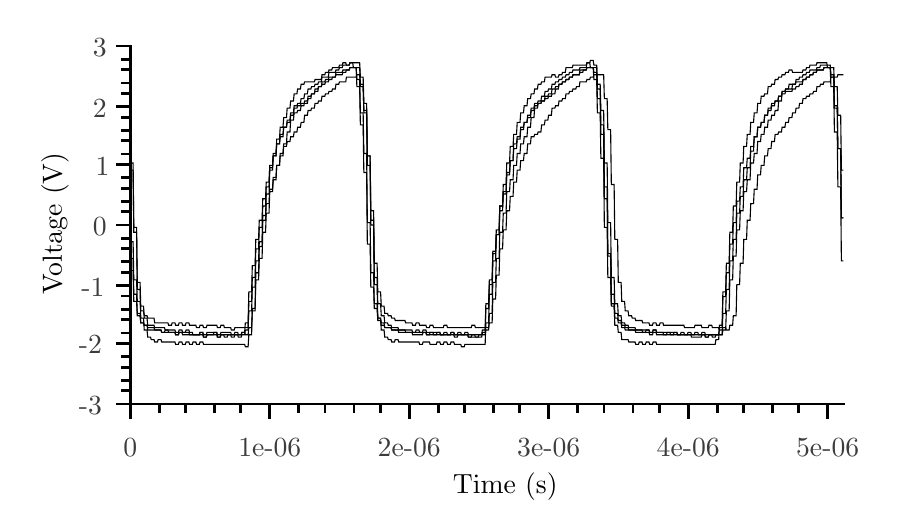
\begin{tikzpicture}{0pt}{0pt}{329pt}{180pt}
	\clip(0pt,180pt) -- (312.853pt,180pt) -- (312.853pt,8.83421pt) -- (0pt,8.83421pt) -- (0pt,180pt);
\begin{scope}
	\clip(37.0859pt,173.344pt) -- (294.786pt,173.344pt) -- (294.786pt,44.0183pt) -- (37.0859pt,44.0183pt) -- (37.0859pt,173.344pt);
	\color[gray]{0}
	\draw[line width=0.4pt, line join=miter, line cap=rect](37.3378pt,96.6106pt) -- (37.5897pt,96.6106pt) -- (37.8416pt,96.6106pt) -- (38.0935pt,96.6106pt) -- (38.3454pt,83.678pt) -- (38.5974pt,83.678pt) -- (38.8493pt,83.678pt) -- (39.1012pt,83.678pt) -- (39.3531pt,83.678pt) -- (39.605pt,76.7807pt) -- (39.8569pt,76.7807pt) -- (40.1088pt,76.7807pt) -- (40.3607pt,76.7807pt) -- (40.6126pt,76.7807pt) -- (40.8645pt,73.332pt) -- (41.1164pt,73.332pt) -- (41.3683pt,73.332pt) -- (41.6202pt,73.332pt) -- (41.8721pt,73.332pt) -- (42.124pt,72.4698pt) -- (42.3759pt,72.4698pt) -- (42.6278pt,72.4698pt) -- (42.8798pt,72.4698pt) -- (43.1317pt,72.4698pt) -- (43.3836pt,70.7455pt) -- (43.6355pt,70.7455pt) -- (43.8874pt,70.7455pt) -- (44.1393pt,70.7455pt) -- (44.3912pt,70.7455pt) -- (44.6431pt,70.7455pt) -- (44.895pt,70.7455pt) -- (45.1469pt,70.7455pt) -- (45.3988pt,70.7455pt) -- (45.6507pt,70.7455pt) -- (45.9026pt,70.7455pt) -- (46.1545pt,70.7455pt) -- (46.4064pt,70.7455pt) -- (46.6583pt,70.7455pt) -- (46.9102pt,70.7455pt) -- (47.1622pt,70.7455pt) -- (47.4141pt,70.7455pt) -- (47.666pt,70.7455pt) -- (47.9179pt,70.7455pt) -- (48.1698pt,70.7455pt) -- (48.4217pt,69.8833pt) -- (48.6736pt,69.8833pt) -- (48.9255pt,69.8833pt) -- (49.1774pt,69.8833pt) -- (49.4293pt,69.8833pt) -- (49.6812pt,69.8833pt) -- (49.9331pt,69.8833pt) -- (50.185pt,69.8833pt) -- (50.4369pt,69.8833pt) -- (50.6888pt,69.8833pt) -- (50.9407pt,69.8833pt) -- (51.1926pt,69.8833pt) -- (51.4446pt,69.8833pt) -- (51.6965pt,69.8833pt) -- (51.9484pt,69.8833pt) -- (52.2003pt,69.8833pt) -- (52.4522pt,69.8833pt) -- (52.7041pt,69.8833pt) -- (52.956pt,69.8833pt) -- (53.2079pt,69.8833pt) -- (53.4598pt,69.0212pt) -- (53.7117pt,69.0212pt) -- (53.9636pt,69.0212pt) -- (54.2155pt,69.0212pt) -- (54.4674pt,69.0212pt) -- (54.7193pt,69.8833pt) -- (54.9712pt,69.8833pt) -- (55.2231pt,69.8833pt) -- (55.475pt,69.8833pt) -- (55.7269pt,69.8833pt) -- (55.9789pt,69.0212pt) -- (56.2308pt,69.0212pt) -- (56.4827pt,69.0212pt) -- (56.7346pt,69.0212pt) -- (56.9865pt,69.0212pt) -- (57.2384pt,69.0212pt) -- (57.4903pt,69.0212pt) -- (57.7422pt,69.0212pt) -- (57.9941pt,69.0212pt) -- (58.246pt,69.0212pt) -- (58.4979pt,69.0212pt) -- (58.7498pt,69.0212pt) -- (59.0017pt,69.0212pt) -- (59.2536pt,69.0212pt) -- (59.5055pt,69.0212pt) -- (59.7574pt,69.0212pt) -- (60.0093pt,69.0212pt) -- (60.2613pt,69.0212pt) -- (60.5132pt,69.0212pt) -- (60.7651pt,69.0212pt) -- (61.017pt,69.0212pt) -- (61.2689pt,69.0212pt) -- (61.5208pt,69.0212pt) -- (61.7727pt,69.0212pt) -- (62.0246pt,69.0212pt) -- (62.2765pt,69.0212pt) -- (62.5284pt,69.0212pt) -- (62.7803pt,69.0212pt) -- (63.0322pt,69.0212pt) -- (63.2841pt,69.0212pt) -- (63.536pt,68.159pt) -- (63.7879pt,68.159pt) -- (64.0398pt,68.159pt) -- (64.2917pt,68.159pt) -- (64.5437pt,68.159pt) -- (64.7956pt,69.0212pt) -- (65.0475pt,69.0212pt) -- (65.2994pt,69.0212pt) -- (65.5513pt,69.0212pt) -- (65.8032pt,69.0212pt) -- (66.0551pt,69.0212pt) -- (66.307pt,69.0212pt) -- (66.5589pt,69.0212pt) -- (66.8108pt,69.0212pt) -- (67.0627pt,69.0212pt) -- (67.3146pt,69.0212pt) -- (67.5665pt,69.0212pt) -- (67.8184pt,69.0212pt) -- (68.0703pt,69.0212pt) -- (68.3222pt,69.0212pt) -- (68.5741pt,68.159pt) -- (68.826pt,68.159pt) -- (69.078pt,68.159pt) -- (69.3299pt,68.159pt) -- (69.5818pt,68.159pt) -- (69.8337pt,69.0212pt) -- (70.0856pt,69.0212pt) -- (70.3375pt,69.0212pt) -- (70.5894pt,69.0212pt) -- (70.8413pt,69.0212pt) -- (71.0932pt,68.159pt) -- (71.3451pt,68.159pt) -- (71.597pt,68.159pt) -- (71.8489pt,68.159pt) -- (72.1008pt,68.159pt) -- (72.3527pt,69.0212pt) -- (72.6046pt,69.0212pt) -- (72.8565pt,69.0212pt) -- (73.1084pt,69.0212pt) -- (73.3604pt,69.0212pt) -- (73.6123pt,68.159pt) -- (73.8642pt,68.159pt) -- (74.1161pt,68.159pt) -- (74.368pt,68.159pt) -- (74.6199pt,68.159pt) -- (74.8718pt,69.0212pt) -- (75.1237pt,69.0212pt) -- (75.3756pt,69.0212pt) -- (75.6275pt,69.0212pt) -- (75.8794pt,69.0212pt) -- (76.1313pt,68.159pt) -- (76.3832pt,68.159pt) -- (76.6351pt,68.159pt) -- (76.887pt,68.159pt) -- (77.1389pt,68.159pt) -- (77.3908pt,69.0212pt) -- (77.6428pt,69.0212pt) -- (77.8947pt,69.0212pt) -- (78.1466pt,69.0212pt) -- (78.3985pt,69.0212pt) -- (78.6504pt,70.7455pt) -- (78.9023pt,70.7455pt) -- (79.1542pt,70.7455pt) -- (79.4061pt,70.7455pt) -- (79.658pt,70.7455pt) -- (79.9099pt,81.0915pt) -- (80.1618pt,81.0915pt) -- (80.4137pt,81.0915pt) -- (80.6656pt,81.0915pt) -- (80.9175pt,81.0915pt) -- (81.1694pt,89.7132pt) -- (81.4213pt,89.7132pt) -- (81.6732pt,89.7132pt) -- (81.9251pt,89.7132pt) -- (82.1771pt,89.7132pt) -- (82.429pt,100.059pt) -- (82.6809pt,100.059pt) -- (82.9328pt,100.059pt) -- (83.1847pt,100.059pt) -- (83.4366pt,100.059pt) -- (83.6885pt,107.819pt) -- (83.9404pt,107.819pt) -- (84.1923pt,107.819pt) -- (84.4442pt,107.819pt) -- (84.6961pt,107.819pt) -- (84.948pt,115.578pt) -- (85.1999pt,115.578pt) -- (85.4518pt,115.578pt) -- (85.7037pt,115.578pt) -- (85.9556pt,115.578pt) -- (86.2075pt,122.476pt) -- (86.4595pt,122.476pt) -- (86.7114pt,122.476pt) -- (86.9633pt,122.476pt) -- (87.2152pt,122.476pt) -- (87.4671pt,130.235pt) -- (87.719pt,130.235pt) -- (87.9709pt,130.235pt) -- (88.2228pt,130.235pt) -- (88.4747pt,130.235pt) -- (88.7266pt,134.546pt) -- (88.9785pt,134.546pt) -- (89.2304pt,134.546pt) -- (89.4823pt,134.546pt) -- (89.7342pt,134.546pt) -- (89.9861pt,137.995pt) -- (90.238pt,137.995pt) -- (90.4899pt,137.995pt) -- (90.7419pt,137.995pt) -- (90.9938pt,137.995pt) -- (91.2457pt,141.443pt) -- (91.4976pt,141.443pt) -- (91.7495pt,141.443pt) -- (92.0014pt,141.443pt) -- (92.2533pt,141.443pt) -- (92.5052pt,144.03pt) -- (92.7571pt,144.03pt) -- (93.009pt,144.03pt) -- (93.2609pt,144.03pt) -- (93.5128pt,144.03pt) -- (93.7647pt,146.616pt) -- (94.0166pt,146.616pt) -- (94.2685pt,146.616pt) -- (94.5204pt,146.616pt) -- (94.7723pt,146.616pt) -- (95.0242pt,149.203pt) -- (95.2762pt,149.203pt) -- (95.5281pt,149.203pt) -- (95.78pt,149.203pt) -- (96.0319pt,149.203pt) -- (96.2838pt,151.789pt) -- (96.5357pt,151.789pt) -- (96.7876pt,151.789pt) -- (97.0395pt,151.789pt) -- (97.2914pt,151.789pt) -- (97.5433pt,152.652pt) -- (97.7952pt,152.652pt) -- (98.0471pt,152.652pt) -- (98.299pt,152.652pt) -- (98.5509pt,152.652pt) -- (98.8028pt,154.376pt) -- (99.0547pt,154.376pt) -- (99.3066pt,154.376pt) -- (99.5586pt,154.376pt) -- (99.8105pt,154.376pt) -- (100.062pt,156.1pt) -- (100.314pt,156.1pt) -- (100.566pt,156.1pt) -- (100.818pt,156.1pt) -- (101.07pt,156.1pt) -- (101.322pt,157.825pt) -- (101.574pt,157.825pt) -- (101.826pt,157.825pt) -- (102.078pt,157.825pt) -- (102.33pt,157.825pt) -- (102.581pt,158.687pt) -- (102.833pt,158.687pt) -- (103.085pt,158.687pt) -- (103.337pt,158.687pt) -- (103.589pt,158.687pt) -- (103.841pt,159.549pt) -- (104.093pt,159.549pt) -- (104.345pt,159.549pt) -- (104.597pt,159.549pt) -- (104.849pt,159.549pt) -- (105.1pt,160.411pt) -- (105.352pt,160.411pt) -- (105.604pt,160.411pt) -- (105.856pt,160.411pt) -- (106.108pt,160.411pt) -- (106.36pt,162.135pt) -- (106.612pt,162.135pt) -- (106.864pt,162.135pt) -- (107.116pt,162.135pt) -- (107.368pt,162.135pt) -- (107.62pt,162.135pt) -- (107.871pt,162.135pt) -- (108.123pt,162.135pt) -- (108.375pt,162.135pt) -- (108.627pt,162.135pt) -- (108.879pt,163.86pt) -- (109.131pt,163.86pt) -- (109.383pt,163.86pt) -- (109.635pt,163.86pt) -- (109.887pt,163.86pt) -- (110.139pt,163.86pt) -- (110.391pt,163.86pt) -- (110.642pt,163.86pt) -- (110.894pt,163.86pt) -- (111.146pt,163.86pt) -- (111.398pt,164.722pt) -- (111.65pt,164.722pt) -- (111.902pt,164.722pt) -- (112.154pt,164.722pt) -- (112.406pt,164.722pt) -- (112.658pt,165.584pt) -- (112.91pt,165.584pt) -- (113.161pt,165.584pt) -- (113.413pt,165.584pt) -- (113.665pt,165.584pt) -- (113.917pt,166.446pt) -- (114.169pt,166.446pt) -- (114.421pt,166.446pt) -- (114.673pt,166.446pt) -- (114.925pt,166.446pt) -- (115.177pt,166.446pt) -- (115.429pt,166.446pt) -- (115.681pt,166.446pt) -- (115.932pt,166.446pt) -- (116.184pt,166.446pt) -- (116.436pt,167.308pt) -- (116.688pt,167.308pt) -- (116.94pt,167.308pt) -- (117.192pt,167.308pt) -- (117.444pt,167.308pt) -- (117.696pt,165.584pt) -- (117.948pt,165.584pt) -- (118.2pt,165.584pt) -- (118.451pt,165.584pt) -- (118.703pt,165.584pt) -- (118.955pt,158.687pt) -- (119.207pt,158.687pt) -- (119.459pt,158.687pt) -- (119.711pt,158.687pt) -- (119.963pt,158.687pt) -- (120.215pt,144.892pt) -- (120.467pt,144.892pt) -- (120.719pt,144.892pt) -- (120.971pt,144.892pt) -- (121.222pt,144.892pt) -- (121.474pt,127.649pt) -- (121.726pt,127.649pt) -- (121.978pt,127.649pt) -- (122.23pt,127.649pt) -- (122.482pt,127.649pt) -- (122.734pt,101.784pt) -- (122.986pt,101.784pt) -- (123.238pt,101.784pt) -- (123.49pt,101.784pt) -- (123.742pt,101.784pt) -- (123.993pt,86.2645pt) -- (124.245pt,86.2645pt) -- (124.497pt,86.2645pt) -- (124.749pt,86.2645pt) -- (125.001pt,86.2645pt) -- (125.253pt,78.505pt) -- (125.505pt,78.505pt) -- (125.757pt,78.505pt) -- (126.009pt,78.505pt) -- (126.261pt,78.505pt) -- (126.512pt,74.1942pt) -- (126.764pt,74.1942pt) -- (127.016pt,74.1942pt) -- (127.268pt,74.1942pt) -- (127.52pt,74.1942pt) -- (127.772pt,72.4698pt) -- (128.024pt,72.4698pt) -- (128.276pt,72.4698pt) -- (128.528pt,72.4698pt) -- (128.78pt,72.4698pt) -- (129.032pt,71.6077pt) -- (129.283pt,71.6077pt) -- (129.535pt,71.6077pt) -- (129.787pt,71.6077pt) -- (130.039pt,71.6077pt) -- (130.291pt,71.6077pt) -- (130.543pt,71.6077pt) -- (130.795pt,71.6077pt) -- (131.047pt,71.6077pt) -- (131.299pt,71.6077pt) -- (131.551pt,70.7455pt) -- (131.802pt,70.7455pt) -- (132.054pt,70.7455pt) -- (132.306pt,70.7455pt) -- (132.558pt,70.7455pt) -- (132.81pt,70.7455pt) -- (133.062pt,70.7455pt) -- (133.314pt,70.7455pt) -- (133.566pt,70.7455pt) -- (133.818pt,70.7455pt) -- (134.07pt,69.8833pt) -- (134.322pt,69.8833pt) -- (134.573pt,69.8833pt) -- (134.825pt,69.8833pt) -- (135.077pt,69.8833pt) -- (135.329pt,69.8833pt) -- (135.581pt,69.8833pt) -- (135.833pt,69.8833pt) -- (136.085pt,69.8833pt) -- (136.337pt,69.8833pt) -- (136.589pt,69.8833pt) -- (136.841pt,69.8833pt) -- (137.093pt,69.8833pt) -- (137.344pt,69.8833pt) -- (137.596pt,69.8833pt) -- (137.848pt,69.8833pt) -- (138.1pt,69.8833pt) -- (138.352pt,69.8833pt) -- (138.604pt,69.8833pt) -- (138.856pt,69.8833pt) -- (139.108pt,69.0212pt) -- (139.36pt,69.0212pt) -- (139.612pt,69.0212pt) -- (139.863pt,69.0212pt) -- (140.115pt,69.0212pt) -- (140.367pt,69.0212pt) -- (140.619pt,69.0212pt) -- (140.871pt,69.0212pt) -- (141.123pt,69.0212pt) -- (141.375pt,69.0212pt) -- (141.627pt,69.0212pt) -- (141.879pt,69.0212pt) -- (142.131pt,69.0212pt) -- (142.383pt,69.0212pt) -- (142.634pt,69.0212pt) -- (142.886pt,69.8833pt) -- (143.138pt,69.8833pt) -- (143.39pt,69.8833pt) -- (143.642pt,69.8833pt) -- (143.894pt,69.8833pt) -- (144.146pt,69.0212pt) -- (144.398pt,69.0212pt) -- (144.65pt,69.0212pt) -- (144.902pt,69.0212pt) -- (145.153pt,69.0212pt) -- (145.405pt,69.0212pt) -- (145.657pt,69.0212pt) -- (145.909pt,69.0212pt) -- (146.161pt,69.0212pt) -- (146.413pt,69.0212pt) -- (146.665pt,69.0212pt) -- (146.917pt,69.0212pt) -- (147.169pt,69.0212pt) -- (147.421pt,69.0212pt) -- (147.673pt,69.0212pt) -- (147.924pt,69.0212pt) -- (148.176pt,69.0212pt) -- (148.428pt,69.0212pt) -- (148.68pt,69.0212pt) -- (148.932pt,69.0212pt) -- (149.184pt,69.0212pt) -- (149.436pt,69.0212pt) -- (149.688pt,69.0212pt) -- (149.94pt,69.0212pt) -- (150.192pt,69.0212pt) -- (150.444pt,69.0212pt) -- (150.695pt,69.0212pt) -- (150.947pt,69.0212pt) -- (151.199pt,69.0212pt) -- (151.451pt,69.0212pt) -- (151.703pt,69.0212pt) -- (151.955pt,69.0212pt) -- (152.207pt,69.0212pt) -- (152.459pt,69.0212pt) -- (152.711pt,69.0212pt) -- (152.963pt,69.0212pt) -- (153.214pt,69.0212pt) -- (153.466pt,69.0212pt) -- (153.718pt,69.0212pt) -- (153.97pt,69.0212pt) -- (154.222pt,68.159pt) -- (154.474pt,68.159pt) -- (154.726pt,68.159pt) -- (154.978pt,68.159pt) -- (155.23pt,68.159pt) -- (155.482pt,69.0212pt) -- (155.734pt,69.0212pt) -- (155.985pt,69.0212pt) -- (156.237pt,69.0212pt) -- (156.489pt,69.0212pt) -- (156.741pt,69.0212pt) -- (156.993pt,69.0212pt) -- (157.245pt,69.0212pt) -- (157.497pt,69.0212pt) -- (157.749pt,69.0212pt) -- (158.001pt,69.0212pt) -- (158.253pt,69.0212pt) -- (158.505pt,69.0212pt) -- (158.756pt,69.0212pt) -- (159.008pt,69.0212pt) -- (159.26pt,68.159pt) -- (159.512pt,68.159pt) -- (159.764pt,68.159pt) -- (160.016pt,68.159pt) -- (160.268pt,68.159pt) -- (160.52pt,68.159pt) -- (160.772pt,68.159pt) -- (161.024pt,68.159pt) -- (161.275pt,68.159pt) -- (161.527pt,68.159pt) -- (161.779pt,68.159pt) -- (162.031pt,68.159pt) -- (162.283pt,68.159pt) -- (162.535pt,68.159pt) -- (162.787pt,68.159pt) -- (163.039pt,68.159pt) -- (163.291pt,68.159pt) -- (163.543pt,68.159pt) -- (163.795pt,68.159pt) -- (164.046pt,68.159pt) -- (164.298pt,69.8833pt) -- (164.55pt,69.8833pt) -- (164.802pt,69.8833pt) -- (165.054pt,69.8833pt) -- (165.306pt,69.8833pt) -- (165.558pt,78.505pt) -- (165.81pt,78.505pt) -- (166.062pt,78.505pt) -- (166.314pt,78.505pt) -- (166.565pt,78.505pt) -- (166.817pt,87.1267pt) -- (167.069pt,87.1267pt) -- (167.321pt,87.1267pt) -- (167.573pt,87.1267pt) -- (167.825pt,87.1267pt) -- (168.077pt,98.3349pt) -- (168.329pt,98.3349pt) -- (168.581pt,98.3349pt) -- (168.833pt,98.3349pt) -- (169.085pt,98.3349pt) -- (169.336pt,105.232pt) -- (169.588pt,105.232pt) -- (169.84pt,105.232pt) -- (170.092pt,105.232pt) -- (170.344pt,105.232pt) -- (170.596pt,113.854pt) -- (170.848pt,113.854pt) -- (171.1pt,113.854pt) -- (171.352pt,113.854pt) -- (171.604pt,113.854pt) -- (171.856pt,119.889pt) -- (172.107pt,119.889pt) -- (172.359pt,119.889pt) -- (172.611pt,119.889pt) -- (172.863pt,119.889pt) -- (173.115pt,126.786pt) -- (173.367pt,126.786pt) -- (173.619pt,126.786pt) -- (173.871pt,126.786pt) -- (174.123pt,126.786pt) -- (174.375pt,131.959pt) -- (174.626pt,131.959pt) -- (174.878pt,131.959pt) -- (175.13pt,131.959pt) -- (175.382pt,131.959pt) -- (175.634pt,137.995pt) -- (175.886pt,137.995pt) -- (176.138pt,137.995pt) -- (176.39pt,137.995pt) -- (176.642pt,137.995pt) -- (176.894pt,140.581pt) -- (177.146pt,140.581pt) -- (177.397pt,140.581pt) -- (177.649pt,140.581pt) -- (177.901pt,140.581pt) -- (178.153pt,144.03pt) -- (178.405pt,144.03pt) -- (178.657pt,144.03pt) -- (178.909pt,144.03pt) -- (179.161pt,144.03pt) -- (179.413pt,145.754pt) -- (179.665pt,145.754pt) -- (179.916pt,145.754pt) -- (180.168pt,145.754pt) -- (180.42pt,145.754pt) -- (180.672pt,148.341pt) -- (180.924pt,148.341pt) -- (181.176pt,148.341pt) -- (181.428pt,148.341pt) -- (181.68pt,148.341pt) -- (181.932pt,150.927pt) -- (182.184pt,150.927pt) -- (182.436pt,150.927pt) -- (182.687pt,150.927pt) -- (182.939pt,150.927pt) -- (183.191pt,152.652pt) -- (183.443pt,152.652pt) -- (183.695pt,152.652pt) -- (183.947pt,152.652pt) -- (184.199pt,152.652pt) -- (184.451pt,153.514pt) -- (184.703pt,153.514pt) -- (184.955pt,153.514pt) -- (185.207pt,153.514pt) -- (185.458pt,153.514pt) -- (185.71pt,155.238pt) -- (185.962pt,155.238pt) -- (186.214pt,155.238pt) -- (186.466pt,155.238pt) -- (186.718pt,155.238pt) -- (186.97pt,156.962pt) -- (187.222pt,156.962pt) -- (187.474pt,156.962pt) -- (187.726pt,156.962pt) -- (187.977pt,156.962pt) -- (188.229pt,157.825pt) -- (188.481pt,157.825pt) -- (188.733pt,157.825pt) -- (188.985pt,157.825pt) -- (189.237pt,157.825pt) -- (189.489pt,159.549pt) -- (189.741pt,159.549pt) -- (189.993pt,159.549pt) -- (190.245pt,159.549pt) -- (190.497pt,159.549pt) -- (190.748pt,160.411pt) -- (191pt,160.411pt) -- (191.252pt,160.411pt) -- (191.504pt,160.411pt) -- (191.756pt,160.411pt) -- (192.008pt,161.273pt) -- (192.26pt,161.273pt) -- (192.512pt,161.273pt) -- (192.764pt,161.273pt) -- (193.016pt,161.273pt) -- (193.267pt,162.135pt) -- (193.519pt,162.135pt) -- (193.771pt,162.135pt) -- (194.023pt,162.135pt) -- (194.275pt,162.135pt) -- (194.527pt,162.998pt) -- (194.779pt,162.998pt) -- (195.031pt,162.998pt) -- (195.283pt,162.998pt) -- (195.535pt,162.998pt) -- (195.787pt,163.86pt) -- (196.038pt,163.86pt) -- (196.29pt,163.86pt) -- (196.542pt,163.86pt) -- (196.794pt,163.86pt) -- (197.046pt,164.722pt) -- (197.298pt,164.722pt) -- (197.55pt,164.722pt) -- (197.802pt,164.722pt) -- (198.054pt,164.722pt) -- (198.306pt,164.722pt) -- (198.558pt,164.722pt) -- (198.809pt,164.722pt) -- (199.061pt,164.722pt) -- (199.313pt,164.722pt) -- (199.565pt,165.584pt) -- (199.817pt,165.584pt) -- (200.069pt,165.584pt) -- (200.321pt,165.584pt) -- (200.573pt,165.584pt) -- (200.825pt,165.584pt) -- (201.077pt,165.584pt) -- (201.328pt,165.584pt) -- (201.58pt,165.584pt) -- (201.832pt,165.584pt) -- (202.084pt,167.308pt) -- (202.336pt,167.308pt) -- (202.588pt,167.308pt) -- (202.84pt,167.308pt) -- (203.092pt,167.308pt) -- (203.344pt,165.584pt) -- (203.596pt,165.584pt) -- (203.848pt,165.584pt) -- (204.099pt,165.584pt) -- (204.351pt,165.584pt) -- (204.603pt,161.273pt) -- (204.855pt,161.273pt) -- (205.107pt,161.273pt) -- (205.359pt,161.273pt) -- (205.611pt,161.273pt) -- (205.863pt,149.203pt) -- (206.115pt,149.203pt) -- (206.367pt,149.203pt) -- (206.619pt,149.203pt) -- (206.87pt,149.203pt) -- (207.122pt,132.822pt) -- (207.374pt,132.822pt) -- (207.626pt,132.822pt) -- (207.878pt,132.822pt) -- (208.13pt,132.822pt) -- (208.382pt,107.819pt) -- (208.634pt,107.819pt) -- (208.886pt,107.819pt) -- (209.138pt,107.819pt) -- (209.389pt,107.819pt) -- (209.641pt,89.7132pt) -- (209.893pt,89.7132pt) -- (210.145pt,89.7132pt) -- (210.397pt,89.7132pt) -- (210.649pt,89.7132pt) -- (210.901pt,79.3672pt) -- (211.153pt,79.3672pt) -- (211.405pt,79.3672pt) -- (211.657pt,79.3672pt) -- (211.909pt,79.3672pt) -- (212.16pt,75.0564pt) -- (212.412pt,75.0564pt) -- (212.664pt,75.0564pt) -- (212.916pt,75.0564pt) -- (213.168pt,75.0564pt) -- (213.42pt,73.332pt) -- (213.672pt,73.332pt) -- (213.924pt,73.332pt) -- (214.176pt,73.332pt) -- (214.428pt,73.332pt) -- (214.679pt,71.6077pt) -- (214.931pt,71.6077pt) -- (215.183pt,71.6077pt) -- (215.435pt,71.6077pt) -- (215.687pt,71.6077pt) -- (215.939pt,70.7455pt) -- (216.191pt,70.7455pt) -- (216.443pt,70.7455pt) -- (216.695pt,70.7455pt) -- (216.947pt,70.7455pt) -- (217.199pt,70.7455pt) -- (217.45pt,70.7455pt) -- (217.702pt,70.7455pt) -- (217.954pt,70.7455pt) -- (218.206pt,70.7455pt) -- (218.458pt,70.7455pt) -- (218.71pt,70.7455pt) -- (218.962pt,70.7455pt) -- (219.214pt,70.7455pt) -- (219.466pt,70.7455pt) -- (219.718pt,69.8833pt) -- (219.97pt,69.8833pt) -- (220.221pt,69.8833pt) -- (220.473pt,69.8833pt) -- (220.725pt,69.8833pt) -- (220.977pt,69.8833pt) -- (221.229pt,69.8833pt) -- (221.481pt,69.8833pt) -- (221.733pt,69.8833pt) -- (221.985pt,69.8833pt) -- (222.237pt,69.8833pt) -- (222.489pt,69.8833pt) -- (222.74pt,69.8833pt) -- (222.992pt,69.8833pt) -- (223.244pt,69.8833pt) -- (223.496pt,69.8833pt) -- (223.748pt,69.8833pt) -- (224pt,69.8833pt) -- (224.252pt,69.8833pt) -- (224.504pt,69.8833pt) -- (224.756pt,69.0212pt) -- (225.008pt,69.0212pt) -- (225.26pt,69.0212pt) -- (225.511pt,69.0212pt) -- (225.763pt,69.0212pt) -- (226.015pt,69.8833pt) -- (226.267pt,69.8833pt) -- (226.519pt,69.8833pt) -- (226.771pt,69.8833pt) -- (227.023pt,69.8833pt) -- (227.275pt,69.0212pt) -- (227.527pt,69.0212pt) -- (227.779pt,69.0212pt) -- (228.03pt,69.0212pt) -- (228.282pt,69.0212pt) -- (228.534pt,69.0212pt) -- (228.786pt,69.0212pt) -- (229.038pt,69.0212pt) -- (229.29pt,69.0212pt) -- (229.542pt,69.0212pt) -- (229.794pt,69.0212pt) -- (230.046pt,69.0212pt) -- (230.298pt,69.0212pt) -- (230.55pt,69.0212pt) -- (230.801pt,69.0212pt) -- (231.053pt,69.0212pt) -- (231.305pt,69.0212pt) -- (231.557pt,69.0212pt) -- (231.809pt,69.0212pt) -- (232.061pt,69.0212pt) -- (232.313pt,69.0212pt) -- (232.565pt,69.0212pt) -- (232.817pt,69.0212pt) -- (233.069pt,69.0212pt) -- (233.321pt,69.0212pt) -- (233.572pt,69.0212pt) -- (233.824pt,69.0212pt) -- (234.076pt,69.0212pt) -- (234.328pt,69.0212pt) -- (234.58pt,69.0212pt) -- (234.832pt,69.0212pt) -- (235.084pt,69.0212pt) -- (235.336pt,69.0212pt) -- (235.588pt,69.0212pt) -- (235.84pt,69.0212pt) -- (236.091pt,69.0212pt) -- (236.343pt,69.0212pt) -- (236.595pt,69.0212pt) -- (236.847pt,69.0212pt) -- (237.099pt,69.0212pt) -- (237.351pt,69.0212pt) -- (237.603pt,69.0212pt) -- (237.855pt,69.0212pt) -- (238.107pt,69.0212pt) -- (238.359pt,69.0212pt) -- (238.611pt,69.0212pt) -- (238.862pt,69.0212pt) -- (239.114pt,69.0212pt) -- (239.366pt,69.0212pt) -- (239.618pt,69.0212pt) -- (239.87pt,68.159pt) -- (240.122pt,68.159pt) -- (240.374pt,68.159pt) -- (240.626pt,68.159pt) -- (240.878pt,68.159pt) -- (241.13pt,68.159pt) -- (241.382pt,68.159pt) -- (241.633pt,68.159pt) -- (241.885pt,68.159pt) -- (242.137pt,68.159pt) -- (242.389pt,68.159pt) -- (242.641pt,68.159pt) -- (242.893pt,68.159pt) -- (243.145pt,68.159pt) -- (243.397pt,68.159pt) -- (243.649pt,69.0212pt) -- (243.901pt,69.0212pt) -- (244.152pt,69.0212pt) -- (244.404pt,69.0212pt) -- (244.656pt,69.0212pt) -- (244.908pt,68.159pt) -- (245.16pt,68.159pt) -- (245.412pt,68.159pt) -- (245.664pt,68.159pt) -- (245.916pt,68.159pt) -- (246.168pt,69.0212pt) -- (246.42pt,69.0212pt) -- (246.672pt,69.0212pt) -- (246.923pt,69.0212pt) -- (247.175pt,69.0212pt) -- (247.427pt,68.159pt) -- (247.679pt,68.159pt) -- (247.931pt,68.159pt) -- (248.183pt,68.159pt) -- (248.435pt,68.159pt) -- (248.687pt,69.0212pt) -- (248.939pt,69.0212pt) -- (249.191pt,69.0212pt) -- (249.442pt,69.0212pt) -- (249.694pt,69.0212pt) -- (249.946pt,69.0212pt) -- (250.198pt,69.0212pt) -- (250.45pt,69.0212pt) -- (250.702pt,69.0212pt) -- (250.954pt,69.0212pt) -- (251.206pt,76.7807pt) -- (251.458pt,76.7807pt) -- (251.71pt,76.7807pt) -- (251.962pt,76.7807pt) -- (252.213pt,76.7807pt) -- (252.465pt,85.4024pt) -- (252.717pt,85.4024pt) -- (252.969pt,85.4024pt) -- (253.221pt,85.4024pt) -- (253.473pt,85.4024pt) -- (253.725pt,95.7484pt) -- (253.977pt,95.7484pt) -- (254.229pt,95.7484pt) -- (254.481pt,95.7484pt) -- (254.733pt,95.7484pt) -- (254.984pt,103.508pt) -- (255.236pt,103.508pt) -- (255.488pt,103.508pt) -- (255.74pt,103.508pt) -- (255.992pt,103.508pt) -- (256.244pt,112.992pt) -- (256.496pt,112.992pt) -- (256.748pt,112.992pt) -- (257pt,112.992pt) -- (257.252pt,112.992pt) -- (257.503pt,119.027pt) -- (257.755pt,119.027pt) -- (258.007pt,119.027pt) -- (258.259pt,119.027pt) -- (258.511pt,119.027pt) -- (258.763pt,125.062pt) -- (259.015pt,125.062pt) -- (259.267pt,125.062pt) -- (259.519pt,125.062pt) -- (259.771pt,125.062pt) -- (260.023pt,129.373pt) -- (260.274pt,129.373pt) -- (260.526pt,129.373pt) -- (260.778pt,129.373pt) -- (261.03pt,129.373pt) -- (261.282pt,135.408pt) -- (261.534pt,135.408pt) -- (261.786pt,135.408pt) -- (262.038pt,135.408pt) -- (262.29pt,135.408pt) -- (262.542pt,140.581pt) -- (262.793pt,140.581pt) -- (263.045pt,140.581pt) -- (263.297pt,140.581pt) -- (263.549pt,140.581pt) -- (263.801pt,144.03pt) -- (264.053pt,144.03pt) -- (264.305pt,144.03pt) -- (264.557pt,144.03pt) -- (264.809pt,144.03pt) -- (265.061pt,145.754pt) -- (265.313pt,145.754pt) -- (265.564pt,145.754pt) -- (265.816pt,145.754pt) -- (266.068pt,145.754pt) -- (266.32pt,148.341pt) -- (266.572pt,148.341pt) -- (266.824pt,148.341pt) -- (267.076pt,148.341pt) -- (267.328pt,148.341pt) -- (267.58pt,150.065pt) -- (267.832pt,150.065pt) -- (268.084pt,150.065pt) -- (268.335pt,150.065pt) -- (268.587pt,150.065pt) -- (268.839pt,151.789pt) -- (269.091pt,151.789pt) -- (269.343pt,151.789pt) -- (269.595pt,151.789pt) -- (269.847pt,151.789pt) -- (270.099pt,153.514pt) -- (270.351pt,153.514pt) -- (270.603pt,153.514pt) -- (270.854pt,153.514pt) -- (271.106pt,153.514pt) -- (271.358pt,155.238pt) -- (271.61pt,155.238pt) -- (271.862pt,155.238pt) -- (272.114pt,155.238pt) -- (272.366pt,155.238pt) -- (272.618pt,156.962pt) -- (272.87pt,156.962pt) -- (273.122pt,156.962pt) -- (273.374pt,156.962pt) -- (273.625pt,156.962pt) -- (273.877pt,157.825pt) -- (274.129pt,157.825pt) -- (274.381pt,157.825pt) -- (274.633pt,157.825pt) -- (274.885pt,157.825pt) -- (275.137pt,159.549pt) -- (275.389pt,159.549pt) -- (275.641pt,159.549pt) -- (275.893pt,159.549pt) -- (276.144pt,159.549pt) -- (276.396pt,159.549pt) -- (276.648pt,159.549pt) -- (276.9pt,159.549pt) -- (277.152pt,159.549pt) -- (277.404pt,159.549pt) -- (277.656pt,161.273pt) -- (277.908pt,161.273pt) -- (278.16pt,161.273pt) -- (278.412pt,161.273pt) -- (278.664pt,161.273pt) -- (278.915pt,162.135pt) -- (279.167pt,162.135pt) -- (279.419pt,162.135pt) -- (279.671pt,162.135pt) -- (279.923pt,162.135pt) -- (280.175pt,162.998pt) -- (280.427pt,162.998pt) -- (280.679pt,162.998pt) -- (280.931pt,162.998pt) -- (281.183pt,162.998pt) -- (281.435pt,163.86pt) -- (281.686pt,163.86pt) -- (281.938pt,163.86pt) -- (282.19pt,163.86pt) -- (282.442pt,163.86pt) -- (282.694pt,164.722pt) -- (282.946pt,164.722pt) -- (283.198pt,164.722pt) -- (283.45pt,164.722pt) -- (283.702pt,164.722pt) -- (283.954pt,164.722pt) -- (284.205pt,164.722pt) -- (284.457pt,164.722pt) -- (284.709pt,164.722pt) -- (284.961pt,164.722pt) -- (285.213pt,165.584pt) -- (285.465pt,165.584pt) -- (285.717pt,165.584pt) -- (285.969pt,165.584pt) -- (286.221pt,165.584pt) -- (286.473pt,166.446pt) -- (286.725pt,166.446pt) -- (286.976pt,166.446pt) -- (287.228pt,166.446pt) -- (287.48pt,166.446pt) -- (287.732pt,166.446pt) -- (287.984pt,166.446pt) -- (288.236pt,166.446pt) -- (288.488pt,166.446pt) -- (288.74pt,166.446pt) -- (288.992pt,166.446pt) -- (289.244pt,166.446pt) -- (289.496pt,166.446pt) -- (289.747pt,166.446pt) -- (289.999pt,166.446pt) -- (290.251pt,162.998pt) -- (290.503pt,162.998pt) -- (290.755pt,162.998pt) -- (291.007pt,162.998pt) -- (291.259pt,162.998pt) -- (291.511pt,151.789pt) -- (291.763pt,151.789pt) -- (292.015pt,151.789pt) -- (292.266pt,151.789pt) -- (292.518pt,151.789pt) -- (292.77pt,136.27pt) -- (293.022pt,136.27pt) -- (293.274pt,136.27pt) -- (293.526pt,136.27pt) -- (293.778pt,136.27pt) -- (294.03pt,111.267pt) -- (294.282pt,111.267pt) -- (294.534pt,111.267pt) -- (294.786pt,111.267pt);
	\color[gray]{0}
	\draw[line width=0.4pt, line join=miter, line cap=rect](37.3378pt,92.2997pt) -- (37.5897pt,92.2997pt) -- (37.8416pt,92.2997pt) -- (38.0935pt,92.2997pt) -- (38.3454pt,81.0915pt) -- (38.5974pt,81.0915pt) -- (38.8493pt,81.0915pt) -- (39.1012pt,81.0915pt) -- (39.3531pt,81.0915pt) -- (39.605pt,75.9185pt) -- (39.8569pt,75.9185pt) -- (40.1088pt,75.9185pt) -- (40.3607pt,75.9185pt) -- (40.6126pt,75.9185pt) -- (40.8645pt,73.332pt) -- (41.1164pt,73.332pt) -- (41.3683pt,73.332pt) -- (41.6202pt,73.332pt) -- (41.8721pt,73.332pt) -- (42.124pt,72.4698pt) -- (42.3759pt,72.4698pt) -- (42.6278pt,72.4698pt) -- (42.8798pt,72.4698pt) -- (43.1317pt,72.4698pt) -- (43.3836pt,71.6077pt) -- (43.6355pt,71.6077pt) -- (43.8874pt,71.6077pt) -- (44.1393pt,71.6077pt) -- (44.3912pt,71.6077pt) -- (44.6431pt,71.6077pt) -- (44.895pt,71.6077pt) -- (45.1469pt,71.6077pt) -- (45.3988pt,71.6077pt) -- (45.6507pt,71.6077pt) -- (45.9026pt,70.7455pt) -- (46.1545pt,70.7455pt) -- (46.4064pt,70.7455pt) -- (46.6583pt,70.7455pt) -- (46.9102pt,70.7455pt) -- (47.1622pt,70.7455pt) -- (47.4141pt,70.7455pt) -- (47.666pt,70.7455pt) -- (47.9179pt,70.7455pt) -- (48.1698pt,70.7455pt) -- (48.4217pt,69.8833pt) -- (48.6736pt,69.8833pt) -- (48.9255pt,69.8833pt) -- (49.1774pt,69.8833pt) -- (49.4293pt,69.8833pt) -- (49.6812pt,70.7455pt) -- (49.9331pt,70.7455pt) -- (50.185pt,70.7455pt) -- (50.4369pt,70.7455pt) -- (50.6888pt,70.7455pt) -- (50.9407pt,69.8833pt) -- (51.1926pt,69.8833pt) -- (51.4446pt,69.8833pt) -- (51.6965pt,69.8833pt) -- (51.9484pt,69.8833pt) -- (52.2003pt,69.8833pt) -- (52.4522pt,69.8833pt) -- (52.7041pt,69.8833pt) -- (52.956pt,69.8833pt) -- (53.2079pt,69.8833pt) -- (53.4598pt,69.0212pt) -- (53.7117pt,69.0212pt) -- (53.9636pt,69.0212pt) -- (54.2155pt,69.0212pt) -- (54.4674pt,69.0212pt) -- (54.7193pt,69.8833pt) -- (54.9712pt,69.8833pt) -- (55.2231pt,69.8833pt) -- (55.475pt,69.8833pt) -- (55.7269pt,69.8833pt) -- (55.9789pt,69.8833pt) -- (56.2308pt,69.8833pt) -- (56.4827pt,69.8833pt) -- (56.7346pt,69.8833pt) -- (56.9865pt,69.8833pt) -- (57.2384pt,69.8833pt) -- (57.4903pt,69.8833pt) -- (57.7422pt,69.8833pt) -- (57.9941pt,69.8833pt) -- (58.246pt,69.8833pt) -- (58.4979pt,69.0212pt) -- (58.7498pt,69.0212pt) -- (59.0017pt,69.0212pt) -- (59.2536pt,69.0212pt) -- (59.5055pt,69.0212pt) -- (59.7574pt,69.0212pt) -- (60.0093pt,69.0212pt) -- (60.2613pt,69.0212pt) -- (60.5132pt,69.0212pt) -- (60.7651pt,69.0212pt) -- (61.017pt,69.0212pt) -- (61.2689pt,69.0212pt) -- (61.5208pt,69.0212pt) -- (61.7727pt,69.0212pt) -- (62.0246pt,69.0212pt) -- (62.2765pt,69.8833pt) -- (62.5284pt,69.8833pt) -- (62.7803pt,69.8833pt) -- (63.0322pt,69.8833pt) -- (63.2841pt,69.8833pt) -- (63.536pt,68.159pt) -- (63.7879pt,68.159pt) -- (64.0398pt,68.159pt) -- (64.2917pt,68.159pt) -- (64.5437pt,68.159pt) -- (64.7956pt,69.0212pt) -- (65.0475pt,69.0212pt) -- (65.2994pt,69.0212pt) -- (65.5513pt,69.0212pt) -- (65.8032pt,69.0212pt) -- (66.0551pt,69.0212pt) -- (66.307pt,69.0212pt) -- (66.5589pt,69.0212pt) -- (66.8108pt,69.0212pt) -- (67.0627pt,69.0212pt) -- (67.3146pt,69.8833pt) -- (67.5665pt,69.8833pt) -- (67.8184pt,69.8833pt) -- (68.0703pt,69.8833pt) -- (68.3222pt,69.8833pt) -- (68.5741pt,68.159pt) -- (68.826pt,68.159pt) -- (69.078pt,68.159pt) -- (69.3299pt,68.159pt) -- (69.5818pt,68.159pt) -- (69.8337pt,69.0212pt) -- (70.0856pt,69.0212pt) -- (70.3375pt,69.0212pt) -- (70.5894pt,69.0212pt) -- (70.8413pt,69.0212pt) -- (71.0932pt,69.0212pt) -- (71.3451pt,69.0212pt) -- (71.597pt,69.0212pt) -- (71.8489pt,69.0212pt) -- (72.1008pt,69.0212pt) -- (72.3527pt,69.0212pt) -- (72.6046pt,69.0212pt) -- (72.8565pt,69.0212pt) -- (73.1084pt,69.0212pt) -- (73.3604pt,69.0212pt) -- (73.6123pt,69.0212pt) -- (73.8642pt,69.0212pt) -- (74.1161pt,69.0212pt) -- (74.368pt,69.0212pt) -- (74.6199pt,69.0212pt) -- (74.8718pt,69.0212pt) -- (75.1237pt,69.0212pt) -- (75.3756pt,69.0212pt) -- (75.6275pt,69.0212pt) -- (75.8794pt,69.0212pt) -- (76.1313pt,69.0212pt) -- (76.3832pt,69.0212pt) -- (76.6351pt,69.0212pt) -- (76.887pt,69.0212pt) -- (77.1389pt,69.0212pt) -- (77.3908pt,69.8833pt) -- (77.6428pt,69.8833pt) -- (77.8947pt,69.8833pt) -- (78.1466pt,69.8833pt) -- (78.3985pt,69.8833pt) -- (78.6504pt,73.332pt) -- (78.9023pt,73.332pt) -- (79.1542pt,73.332pt) -- (79.4061pt,73.332pt) -- (79.658pt,73.332pt) -- (79.9099pt,84.5402pt) -- (80.1618pt,84.5402pt) -- (80.4137pt,84.5402pt) -- (80.6656pt,84.5402pt) -- (80.9175pt,84.5402pt) -- (81.1694pt,94.0241pt) -- (81.4213pt,94.0241pt) -- (81.6732pt,94.0241pt) -- (81.9251pt,94.0241pt) -- (82.1771pt,94.0241pt) -- (82.429pt,103.508pt) -- (82.6809pt,103.508pt) -- (82.9328pt,103.508pt) -- (83.1847pt,103.508pt) -- (83.4366pt,103.508pt) -- (83.6885pt,110.405pt) -- (83.9404pt,110.405pt) -- (84.1923pt,110.405pt) -- (84.4442pt,110.405pt) -- (84.6961pt,110.405pt) -- (84.948pt,118.165pt) -- (85.1999pt,118.165pt) -- (85.4518pt,118.165pt) -- (85.7037pt,118.165pt) -- (85.9556pt,118.165pt) -- (86.2075pt,124.2pt) -- (86.4595pt,124.2pt) -- (86.7114pt,124.2pt) -- (86.9633pt,124.2pt) -- (87.2152pt,124.2pt) -- (87.4671pt,129.373pt) -- (87.719pt,129.373pt) -- (87.9709pt,129.373pt) -- (88.2228pt,129.373pt) -- (88.4747pt,129.373pt) -- (88.7266pt,133.684pt) -- (88.9785pt,133.684pt) -- (89.2304pt,133.684pt) -- (89.4823pt,133.684pt) -- (89.7342pt,133.684pt) -- (89.9861pt,137.995pt) -- (90.238pt,137.995pt) -- (90.4899pt,137.995pt) -- (90.7419pt,137.995pt) -- (90.9938pt,137.995pt) -- (91.2457pt,140.581pt) -- (91.4976pt,140.581pt) -- (91.7495pt,140.581pt) -- (92.0014pt,140.581pt) -- (92.2533pt,140.581pt) -- (92.5052pt,144.03pt) -- (92.7571pt,144.03pt) -- (93.009pt,144.03pt) -- (93.2609pt,144.03pt) -- (93.5128pt,144.03pt) -- (93.7647pt,145.754pt) -- (94.0166pt,145.754pt) -- (94.2685pt,145.754pt) -- (94.5204pt,145.754pt) -- (94.7723pt,145.754pt) -- (95.0242pt,148.341pt) -- (95.2762pt,148.341pt) -- (95.5281pt,148.341pt) -- (95.78pt,148.341pt) -- (96.0319pt,148.341pt) -- (96.2838pt,150.927pt) -- (96.5357pt,150.927pt) -- (96.7876pt,150.927pt) -- (97.0395pt,150.927pt) -- (97.2914pt,150.927pt) -- (97.5433pt,151.789pt) -- (97.7952pt,151.789pt) -- (98.0471pt,151.789pt) -- (98.299pt,151.789pt) -- (98.5509pt,151.789pt) -- (98.8028pt,152.652pt) -- (99.0547pt,152.652pt) -- (99.3066pt,152.652pt) -- (99.5586pt,152.652pt) -- (99.8105pt,152.652pt) -- (100.062pt,152.652pt) -- (100.314pt,152.652pt) -- (100.566pt,152.652pt) -- (100.818pt,152.652pt) -- (101.07pt,152.652pt) -- (101.322pt,154.376pt) -- (101.574pt,154.376pt) -- (101.826pt,154.376pt) -- (102.078pt,154.376pt) -- (102.33pt,154.376pt) -- (102.581pt,156.1pt) -- (102.833pt,156.1pt) -- (103.085pt,156.1pt) -- (103.337pt,156.1pt) -- (103.589pt,156.1pt) -- (103.841pt,157.825pt) -- (104.093pt,157.825pt) -- (104.345pt,157.825pt) -- (104.597pt,157.825pt) -- (104.849pt,157.825pt) -- (105.1pt,158.687pt) -- (105.352pt,158.687pt) -- (105.604pt,158.687pt) -- (105.856pt,158.687pt) -- (106.108pt,158.687pt) -- (106.36pt,160.411pt) -- (106.612pt,160.411pt) -- (106.864pt,160.411pt) -- (107.116pt,160.411pt) -- (107.368pt,160.411pt) -- (107.62pt,161.273pt) -- (107.871pt,161.273pt) -- (108.123pt,161.273pt) -- (108.375pt,161.273pt) -- (108.627pt,161.273pt) -- (108.879pt,162.135pt) -- (109.131pt,162.135pt) -- (109.383pt,162.135pt) -- (109.635pt,162.135pt) -- (109.887pt,162.135pt) -- (110.139pt,162.135pt) -- (110.391pt,162.135pt) -- (110.642pt,162.135pt) -- (110.894pt,162.135pt) -- (111.146pt,162.135pt) -- (111.398pt,163.86pt) -- (111.65pt,163.86pt) -- (111.902pt,163.86pt) -- (112.154pt,163.86pt) -- (112.406pt,163.86pt) -- (112.658pt,163.86pt) -- (112.91pt,163.86pt) -- (113.161pt,163.86pt) -- (113.413pt,163.86pt) -- (113.665pt,163.86pt) -- (113.917pt,164.722pt) -- (114.169pt,164.722pt) -- (114.421pt,164.722pt) -- (114.673pt,164.722pt) -- (114.925pt,164.722pt) -- (115.177pt,164.722pt) -- (115.429pt,164.722pt) -- (115.681pt,164.722pt) -- (115.932pt,164.722pt) -- (116.184pt,164.722pt) -- (116.436pt,165.584pt) -- (116.688pt,165.584pt) -- (116.94pt,165.584pt) -- (117.192pt,165.584pt) -- (117.444pt,165.584pt) -- (117.696pt,165.584pt) -- (117.948pt,165.584pt) -- (118.2pt,165.584pt) -- (118.451pt,165.584pt) -- (118.703pt,165.584pt) -- (118.955pt,161.273pt) -- (119.207pt,161.273pt) -- (119.459pt,161.273pt) -- (119.711pt,161.273pt) -- (119.963pt,161.273pt) -- (120.215pt,149.203pt) -- (120.467pt,149.203pt) -- (120.719pt,149.203pt) -- (120.971pt,149.203pt) -- (121.222pt,149.203pt) -- (121.474pt,134.546pt) -- (121.726pt,134.546pt) -- (121.978pt,134.546pt) -- (122.23pt,134.546pt) -- (122.482pt,134.546pt) -- (122.734pt,109.543pt) -- (122.986pt,109.543pt) -- (123.238pt,109.543pt) -- (123.49pt,109.543pt) -- (123.742pt,109.543pt) -- (123.993pt,91.4376pt) -- (124.245pt,91.4376pt) -- (124.497pt,91.4376pt) -- (124.749pt,91.4376pt) -- (125.001pt,91.4376pt) -- (125.253pt,80.2294pt) -- (125.505pt,80.2294pt) -- (125.757pt,80.2294pt) -- (126.009pt,80.2294pt) -- (126.261pt,80.2294pt) -- (126.512pt,75.0564pt) -- (126.764pt,75.0564pt) -- (127.016pt,75.0564pt) -- (127.268pt,75.0564pt) -- (127.52pt,75.0564pt) -- (127.772pt,73.332pt) -- (128.024pt,73.332pt) -- (128.276pt,73.332pt) -- (128.528pt,73.332pt) -- (128.78pt,73.332pt) -- (129.032pt,71.6077pt) -- (129.283pt,71.6077pt) -- (129.535pt,71.6077pt) -- (129.787pt,71.6077pt) -- (130.039pt,71.6077pt) -- (130.291pt,71.6077pt) -- (130.543pt,71.6077pt) -- (130.795pt,71.6077pt) -- (131.047pt,71.6077pt) -- (131.299pt,71.6077pt) -- (131.551pt,70.7455pt) -- (131.802pt,70.7455pt) -- (132.054pt,70.7455pt) -- (132.306pt,70.7455pt) -- (132.558pt,70.7455pt) -- (132.81pt,70.7455pt) -- (133.062pt,70.7455pt) -- (133.314pt,70.7455pt) -- (133.566pt,70.7455pt) -- (133.818pt,70.7455pt) -- (134.07pt,70.7455pt) -- (134.322pt,70.7455pt) -- (134.573pt,70.7455pt) -- (134.825pt,70.7455pt) -- (135.077pt,70.7455pt) -- (135.329pt,70.7455pt) -- (135.581pt,70.7455pt) -- (135.833pt,70.7455pt) -- (136.085pt,70.7455pt) -- (136.337pt,70.7455pt) -- (136.589pt,69.8833pt) -- (136.841pt,69.8833pt) -- (137.093pt,69.8833pt) -- (137.344pt,69.8833pt) -- (137.596pt,69.8833pt) -- (137.848pt,69.8833pt) -- (138.1pt,69.8833pt) -- (138.352pt,69.8833pt) -- (138.604pt,69.8833pt) -- (138.856pt,69.8833pt) -- (139.108pt,69.8833pt) -- (139.36pt,69.8833pt) -- (139.612pt,69.8833pt) -- (139.863pt,69.8833pt) -- (140.115pt,69.8833pt) -- (140.367pt,69.8833pt) -- (140.619pt,69.8833pt) -- (140.871pt,69.8833pt) -- (141.123pt,69.8833pt) -- (141.375pt,69.8833pt) -- (141.627pt,69.8833pt) -- (141.879pt,69.8833pt) -- (142.131pt,69.8833pt) -- (142.383pt,69.8833pt) -- (142.634pt,69.8833pt) -- (142.886pt,69.8833pt) -- (143.138pt,69.8833pt) -- (143.39pt,69.8833pt) -- (143.642pt,69.8833pt) -- (143.894pt,69.8833pt) -- (144.146pt,69.0212pt) -- (144.398pt,69.0212pt) -- (144.65pt,69.0212pt) -- (144.902pt,69.0212pt) -- (145.153pt,69.0212pt) -- (145.405pt,69.8833pt) -- (145.657pt,69.8833pt) -- (145.909pt,69.8833pt) -- (146.161pt,69.8833pt) -- (146.413pt,69.8833pt) -- (146.665pt,69.0212pt) -- (146.917pt,69.0212pt) -- (147.169pt,69.0212pt) -- (147.421pt,69.0212pt) -- (147.673pt,69.0212pt) -- (147.924pt,69.8833pt) -- (148.176pt,69.8833pt) -- (148.428pt,69.8833pt) -- (148.68pt,69.8833pt) -- (148.932pt,69.8833pt) -- (149.184pt,69.0212pt) -- (149.436pt,69.0212pt) -- (149.688pt,69.0212pt) -- (149.94pt,69.0212pt) -- (150.192pt,69.0212pt) -- (150.444pt,69.0212pt) -- (150.695pt,69.0212pt) -- (150.947pt,69.0212pt) -- (151.199pt,69.0212pt) -- (151.451pt,69.0212pt) -- (151.703pt,69.0212pt) -- (151.955pt,69.0212pt) -- (152.207pt,69.0212pt) -- (152.459pt,69.0212pt) -- (152.711pt,69.0212pt) -- (152.963pt,69.8833pt) -- (153.214pt,69.8833pt) -- (153.466pt,69.8833pt) -- (153.718pt,69.8833pt) -- (153.97pt,69.8833pt) -- (154.222pt,69.0212pt) -- (154.474pt,69.0212pt) -- (154.726pt,69.0212pt) -- (154.978pt,69.0212pt) -- (155.23pt,69.0212pt) -- (155.482pt,69.0212pt) -- (155.734pt,69.0212pt) -- (155.985pt,69.0212pt) -- (156.237pt,69.0212pt) -- (156.489pt,69.0212pt) -- (156.741pt,69.0212pt) -- (156.993pt,69.0212pt) -- (157.245pt,69.0212pt) -- (157.497pt,69.0212pt) -- (157.749pt,69.0212pt) -- (158.001pt,69.0212pt) -- (158.253pt,69.0212pt) -- (158.505pt,69.0212pt) -- (158.756pt,69.0212pt) -- (159.008pt,69.0212pt) -- (159.26pt,68.159pt) -- (159.512pt,68.159pt) -- (159.764pt,68.159pt) -- (160.016pt,68.159pt) -- (160.268pt,68.159pt) -- (160.52pt,69.0212pt) -- (160.772pt,69.0212pt) -- (161.024pt,69.0212pt) -- (161.275pt,69.0212pt) -- (161.527pt,69.0212pt) -- (161.779pt,68.159pt) -- (162.031pt,68.159pt) -- (162.283pt,68.159pt) -- (162.535pt,68.159pt) -- (162.787pt,68.159pt) -- (163.039pt,69.0212pt) -- (163.291pt,69.0212pt) -- (163.543pt,69.0212pt) -- (163.795pt,69.0212pt) -- (164.046pt,69.0212pt) -- (164.298pt,70.7455pt) -- (164.55pt,70.7455pt) -- (164.802pt,70.7455pt) -- (165.054pt,70.7455pt) -- (165.306pt,70.7455pt) -- (165.558pt,80.2294pt) -- (165.81pt,80.2294pt) -- (166.062pt,80.2294pt) -- (166.314pt,80.2294pt) -- (166.565pt,80.2294pt) -- (166.817pt,88.851pt) -- (167.069pt,88.851pt) -- (167.321pt,88.851pt) -- (167.573pt,88.851pt) -- (167.825pt,88.851pt) -- (168.077pt,99.1971pt) -- (168.329pt,99.1971pt) -- (168.581pt,99.1971pt) -- (168.833pt,99.1971pt) -- (169.085pt,99.1971pt) -- (169.336pt,106.957pt) -- (169.588pt,106.957pt) -- (169.84pt,106.957pt) -- (170.092pt,106.957pt) -- (170.344pt,106.957pt) -- (170.596pt,115.578pt) -- (170.848pt,115.578pt) -- (171.1pt,115.578pt) -- (171.352pt,115.578pt) -- (171.604pt,115.578pt) -- (171.856pt,120.751pt) -- (172.107pt,120.751pt) -- (172.359pt,120.751pt) -- (172.611pt,120.751pt) -- (172.863pt,120.751pt) -- (173.115pt,127.649pt) -- (173.367pt,127.649pt) -- (173.619pt,127.649pt) -- (173.871pt,127.649pt) -- (174.123pt,127.649pt) -- (174.375pt,131.959pt) -- (174.626pt,131.959pt) -- (174.878pt,131.959pt) -- (175.13pt,131.959pt) -- (175.382pt,131.959pt) -- (175.634pt,136.27pt) -- (175.886pt,136.27pt) -- (176.138pt,136.27pt) -- (176.39pt,136.27pt) -- (176.642pt,136.27pt) -- (176.894pt,139.719pt) -- (177.146pt,139.719pt) -- (177.397pt,139.719pt) -- (177.649pt,139.719pt) -- (177.901pt,139.719pt) -- (178.153pt,143.168pt) -- (178.405pt,143.168pt) -- (178.657pt,143.168pt) -- (178.909pt,143.168pt) -- (179.161pt,143.168pt) -- (179.413pt,145.754pt) -- (179.665pt,145.754pt) -- (179.916pt,145.754pt) -- (180.168pt,145.754pt) -- (180.42pt,145.754pt) -- (180.672pt,147.478pt) -- (180.924pt,147.478pt) -- (181.176pt,147.478pt) -- (181.428pt,147.478pt) -- (181.68pt,147.478pt) -- (181.932pt,150.065pt) -- (182.184pt,150.065pt) -- (182.436pt,150.065pt) -- (182.687pt,150.065pt) -- (182.939pt,150.065pt) -- (183.191pt,151.789pt) -- (183.443pt,151.789pt) -- (183.695pt,151.789pt) -- (183.947pt,151.789pt) -- (184.199pt,151.789pt) -- (184.451pt,152.652pt) -- (184.703pt,152.652pt) -- (184.955pt,152.652pt) -- (185.207pt,152.652pt) -- (185.458pt,152.652pt) -- (185.71pt,153.514pt) -- (185.962pt,153.514pt) -- (186.214pt,153.514pt) -- (186.466pt,153.514pt) -- (186.718pt,153.514pt) -- (186.97pt,154.376pt) -- (187.222pt,154.376pt) -- (187.474pt,154.376pt) -- (187.726pt,154.376pt) -- (187.977pt,154.376pt) -- (188.229pt,155.238pt) -- (188.481pt,155.238pt) -- (188.733pt,155.238pt) -- (188.985pt,155.238pt) -- (189.237pt,155.238pt) -- (189.489pt,156.1pt) -- (189.741pt,156.1pt) -- (189.993pt,156.1pt) -- (190.245pt,156.1pt) -- (190.497pt,156.1pt) -- (190.748pt,157.825pt) -- (191pt,157.825pt) -- (191.252pt,157.825pt) -- (191.504pt,157.825pt) -- (191.756pt,157.825pt) -- (192.008pt,159.549pt) -- (192.26pt,159.549pt) -- (192.512pt,159.549pt) -- (192.764pt,159.549pt) -- (193.016pt,159.549pt) -- (193.267pt,160.411pt) -- (193.519pt,160.411pt) -- (193.771pt,160.411pt) -- (194.023pt,160.411pt) -- (194.275pt,160.411pt) -- (194.527pt,161.273pt) -- (194.779pt,161.273pt) -- (195.031pt,161.273pt) -- (195.283pt,161.273pt) -- (195.535pt,161.273pt) -- (195.787pt,162.135pt) -- (196.038pt,162.135pt) -- (196.29pt,162.135pt) -- (196.542pt,162.135pt) -- (196.794pt,162.135pt) -- (197.046pt,162.998pt) -- (197.298pt,162.998pt) -- (197.55pt,162.998pt) -- (197.802pt,162.998pt) -- (198.054pt,162.998pt) -- (198.306pt,162.998pt) -- (198.558pt,162.998pt) -- (198.809pt,162.998pt) -- (199.061pt,162.998pt) -- (199.313pt,162.998pt) -- (199.565pt,164.722pt) -- (199.817pt,164.722pt) -- (200.069pt,164.722pt) -- (200.321pt,164.722pt) -- (200.573pt,164.722pt) -- (200.825pt,164.722pt) -- (201.077pt,164.722pt) -- (201.328pt,164.722pt) -- (201.58pt,164.722pt) -- (201.832pt,164.722pt) -- (202.084pt,165.584pt) -- (202.336pt,165.584pt) -- (202.588pt,165.584pt) -- (202.84pt,165.584pt) -- (203.092pt,165.584pt) -- (203.344pt,165.584pt) -- (203.596pt,165.584pt) -- (203.848pt,165.584pt) -- (204.099pt,165.584pt) -- (204.351pt,165.584pt) -- (204.603pt,163.86pt) -- (204.855pt,163.86pt) -- (205.107pt,163.86pt) -- (205.359pt,163.86pt) -- (205.611pt,163.86pt) -- (205.863pt,154.376pt) -- (206.115pt,154.376pt) -- (206.367pt,154.376pt) -- (206.619pt,154.376pt) -- (206.87pt,154.376pt) -- (207.122pt,141.443pt) -- (207.374pt,141.443pt) -- (207.626pt,141.443pt) -- (207.878pt,141.443pt) -- (208.13pt,141.443pt) -- (208.382pt,118.165pt) -- (208.634pt,118.165pt) -- (208.886pt,118.165pt) -- (209.138pt,118.165pt) -- (209.389pt,118.165pt) -- (209.641pt,97.4727pt) -- (209.893pt,97.4727pt) -- (210.145pt,97.4727pt) -- (210.397pt,97.4727pt) -- (210.649pt,97.4727pt) -- (210.901pt,83.678pt) -- (211.153pt,83.678pt) -- (211.405pt,83.678pt) -- (211.657pt,83.678pt) -- (211.909pt,83.678pt) -- (212.16pt,76.7807pt) -- (212.412pt,76.7807pt) -- (212.664pt,76.7807pt) -- (212.916pt,76.7807pt) -- (213.168pt,76.7807pt) -- (213.42pt,74.1942pt) -- (213.672pt,74.1942pt) -- (213.924pt,74.1942pt) -- (214.176pt,74.1942pt) -- (214.428pt,74.1942pt) -- (214.679pt,72.4698pt) -- (214.931pt,72.4698pt) -- (215.183pt,72.4698pt) -- (215.435pt,72.4698pt) -- (215.687pt,72.4698pt) -- (215.939pt,71.6077pt) -- (216.191pt,71.6077pt) -- (216.443pt,71.6077pt) -- (216.695pt,71.6077pt) -- (216.947pt,71.6077pt) -- (217.199pt,70.7455pt) -- (217.45pt,70.7455pt) -- (217.702pt,70.7455pt) -- (217.954pt,70.7455pt) -- (218.206pt,70.7455pt) -- (218.458pt,70.7455pt) -- (218.71pt,70.7455pt) -- (218.962pt,70.7455pt) -- (219.214pt,70.7455pt) -- (219.466pt,70.7455pt) -- (219.718pt,70.7455pt) -- (219.97pt,70.7455pt) -- (220.221pt,70.7455pt) -- (220.473pt,70.7455pt) -- (220.725pt,70.7455pt) -- (220.977pt,70.7455pt) -- (221.229pt,70.7455pt) -- (221.481pt,70.7455pt) -- (221.733pt,70.7455pt) -- (221.985pt,70.7455pt) -- (222.237pt,69.8833pt) -- (222.489pt,69.8833pt) -- (222.74pt,69.8833pt) -- (222.992pt,69.8833pt) -- (223.244pt,69.8833pt) -- (223.496pt,70.7455pt) -- (223.748pt,70.7455pt) -- (224pt,70.7455pt) -- (224.252pt,70.7455pt) -- (224.504pt,70.7455pt) -- (224.756pt,69.8833pt) -- (225.008pt,69.8833pt) -- (225.26pt,69.8833pt) -- (225.511pt,69.8833pt) -- (225.763pt,69.8833pt) -- (226.015pt,70.7455pt) -- (226.267pt,70.7455pt) -- (226.519pt,70.7455pt) -- (226.771pt,70.7455pt) -- (227.023pt,70.7455pt) -- (227.275pt,69.8833pt) -- (227.527pt,69.8833pt) -- (227.779pt,69.8833pt) -- (228.03pt,69.8833pt) -- (228.282pt,69.8833pt) -- (228.534pt,69.8833pt) -- (228.786pt,69.8833pt) -- (229.038pt,69.8833pt) -- (229.29pt,69.8833pt) -- (229.542pt,69.8833pt) -- (229.794pt,69.0212pt) -- (230.046pt,69.0212pt) -- (230.298pt,69.0212pt) -- (230.55pt,69.0212pt) -- (230.801pt,69.0212pt) -- (231.053pt,69.8833pt) -- (231.305pt,69.8833pt) -- (231.557pt,69.8833pt) -- (231.809pt,69.8833pt) -- (232.061pt,69.8833pt) -- (232.313pt,69.0212pt) -- (232.565pt,69.0212pt) -- (232.817pt,69.0212pt) -- (233.069pt,69.0212pt) -- (233.321pt,69.0212pt) -- (233.572pt,69.8833pt) -- (233.824pt,69.8833pt) -- (234.076pt,69.8833pt) -- (234.328pt,69.8833pt) -- (234.58pt,69.8833pt) -- (234.832pt,69.0212pt) -- (235.084pt,69.0212pt) -- (235.336pt,69.0212pt) -- (235.588pt,69.0212pt) -- (235.84pt,69.0212pt) -- (236.091pt,69.0212pt) -- (236.343pt,69.0212pt) -- (236.595pt,69.0212pt) -- (236.847pt,69.0212pt) -- (237.099pt,69.0212pt) -- (237.351pt,69.0212pt) -- (237.603pt,69.0212pt) -- (237.855pt,69.0212pt) -- (238.107pt,69.0212pt) -- (238.359pt,69.0212pt) -- (238.611pt,69.0212pt) -- (238.862pt,69.0212pt) -- (239.114pt,69.0212pt) -- (239.366pt,69.0212pt) -- (239.618pt,69.0212pt) -- (239.87pt,69.0212pt) -- (240.122pt,69.0212pt) -- (240.374pt,69.0212pt) -- (240.626pt,69.0212pt) -- (240.878pt,69.0212pt) -- (241.13pt,69.0212pt) -- (241.382pt,69.0212pt) -- (241.633pt,69.0212pt) -- (241.885pt,69.0212pt) -- (242.137pt,69.0212pt) -- (242.389pt,69.0212pt) -- (242.641pt,69.0212pt) -- (242.893pt,69.0212pt) -- (243.145pt,69.0212pt) -- (243.397pt,69.0212pt) -- (243.649pt,69.0212pt) -- (243.901pt,69.0212pt) -- (244.152pt,69.0212pt) -- (244.404pt,69.0212pt) -- (244.656pt,69.0212pt) -- (244.908pt,68.159pt) -- (245.16pt,68.159pt) -- (245.412pt,68.159pt) -- (245.664pt,68.159pt) -- (245.916pt,68.159pt) -- (246.168pt,69.0212pt) -- (246.42pt,69.0212pt) -- (246.672pt,69.0212pt) -- (246.923pt,69.0212pt) -- (247.175pt,69.0212pt) -- (247.427pt,69.0212pt) -- (247.679pt,69.0212pt) -- (247.931pt,69.0212pt) -- (248.183pt,69.0212pt) -- (248.435pt,69.0212pt) -- (248.687pt,69.0212pt) -- (248.939pt,69.0212pt) -- (249.191pt,69.0212pt) -- (249.442pt,69.0212pt) -- (249.694pt,69.0212pt) -- (249.946pt,71.6077pt) -- (250.198pt,71.6077pt) -- (250.45pt,71.6077pt) -- (250.702pt,71.6077pt) -- (250.954pt,71.6077pt) -- (251.206pt,82.8159pt) -- (251.458pt,82.8159pt) -- (251.71pt,82.8159pt) -- (251.962pt,82.8159pt) -- (252.213pt,82.8159pt) -- (252.465pt,91.4376pt) -- (252.717pt,91.4376pt) -- (252.969pt,91.4376pt) -- (253.221pt,91.4376pt) -- (253.473pt,91.4376pt) -- (253.725pt,101.784pt) -- (253.977pt,101.784pt) -- (254.229pt,101.784pt) -- (254.481pt,101.784pt) -- (254.733pt,101.784pt) -- (254.984pt,109.543pt) -- (255.236pt,109.543pt) -- (255.488pt,109.543pt) -- (255.74pt,109.543pt) -- (255.992pt,109.543pt) -- (256.244pt,117.303pt) -- (256.496pt,117.303pt) -- (256.748pt,117.303pt) -- (257pt,117.303pt) -- (257.252pt,117.303pt) -- (257.503pt,122.476pt) -- (257.755pt,122.476pt) -- (258.007pt,122.476pt) -- (258.259pt,122.476pt) -- (258.511pt,122.476pt) -- (258.763pt,129.373pt) -- (259.015pt,129.373pt) -- (259.267pt,129.373pt) -- (259.519pt,129.373pt) -- (259.771pt,129.373pt) -- (260.023pt,132.822pt) -- (260.274pt,132.822pt) -- (260.526pt,132.822pt) -- (260.778pt,132.822pt) -- (261.03pt,132.822pt) -- (261.282pt,137.132pt) -- (261.534pt,137.132pt) -- (261.786pt,137.132pt) -- (262.038pt,137.132pt) -- (262.29pt,137.132pt) -- (262.542pt,140.581pt) -- (262.793pt,140.581pt) -- (263.045pt,140.581pt) -- (263.297pt,140.581pt) -- (263.549pt,140.581pt) -- (263.801pt,144.03pt) -- (264.053pt,144.03pt) -- (264.305pt,144.03pt) -- (264.557pt,144.03pt) -- (264.809pt,144.03pt) -- (265.061pt,145.754pt) -- (265.313pt,145.754pt) -- (265.564pt,145.754pt) -- (265.816pt,145.754pt) -- (266.068pt,145.754pt) -- (266.32pt,148.341pt) -- (266.572pt,148.341pt) -- (266.824pt,148.341pt) -- (267.076pt,148.341pt) -- (267.328pt,148.341pt) -- (267.58pt,150.927pt) -- (267.832pt,150.927pt) -- (268.084pt,150.927pt) -- (268.335pt,150.927pt) -- (268.587pt,150.927pt) -- (268.839pt,152.652pt) -- (269.091pt,152.652pt) -- (269.343pt,152.652pt) -- (269.595pt,152.652pt) -- (269.847pt,152.652pt) -- (270.099pt,153.514pt) -- (270.351pt,153.514pt) -- (270.603pt,153.514pt) -- (270.854pt,153.514pt) -- (271.106pt,153.514pt) -- (271.358pt,155.238pt) -- (271.61pt,155.238pt) -- (271.862pt,155.238pt) -- (272.114pt,155.238pt) -- (272.366pt,155.238pt) -- (272.618pt,156.1pt) -- (272.87pt,156.1pt) -- (273.122pt,156.1pt) -- (273.374pt,156.1pt) -- (273.625pt,156.1pt) -- (273.877pt,156.962pt) -- (274.129pt,156.962pt) -- (274.381pt,156.962pt) -- (274.633pt,156.962pt) -- (274.885pt,156.962pt) -- (275.137pt,156.962pt) -- (275.389pt,156.962pt) -- (275.641pt,156.962pt) -- (275.893pt,156.962pt) -- (276.144pt,156.962pt) -- (276.396pt,157.825pt) -- (276.648pt,157.825pt) -- (276.9pt,157.825pt) -- (277.152pt,157.825pt) -- (277.404pt,157.825pt) -- (277.656pt,158.687pt) -- (277.908pt,158.687pt) -- (278.16pt,158.687pt) -- (278.412pt,158.687pt) -- (278.664pt,158.687pt) -- (278.915pt,159.549pt) -- (279.167pt,159.549pt) -- (279.419pt,159.549pt) -- (279.671pt,159.549pt) -- (279.923pt,159.549pt) -- (280.175pt,161.273pt) -- (280.427pt,161.273pt) -- (280.679pt,161.273pt) -- (280.931pt,161.273pt) -- (281.183pt,161.273pt) -- (281.435pt,162.135pt) -- (281.686pt,162.135pt) -- (281.938pt,162.135pt) -- (282.19pt,162.135pt) -- (282.442pt,162.135pt) -- (282.694pt,162.998pt) -- (282.946pt,162.998pt) -- (283.198pt,162.998pt) -- (283.45pt,162.998pt) -- (283.702pt,162.998pt) -- (283.954pt,163.86pt) -- (284.205pt,163.86pt) -- (284.457pt,163.86pt) -- (284.709pt,163.86pt) -- (284.961pt,163.86pt) -- (285.213pt,164.722pt) -- (285.465pt,164.722pt) -- (285.717pt,164.722pt) -- (285.969pt,164.722pt) -- (286.221pt,164.722pt) -- (286.473pt,164.722pt) -- (286.725pt,164.722pt) -- (286.976pt,164.722pt) -- (287.228pt,164.722pt) -- (287.48pt,164.722pt) -- (287.732pt,165.584pt) -- (287.984pt,165.584pt) -- (288.236pt,165.584pt) -- (288.488pt,165.584pt) -- (288.74pt,165.584pt) -- (288.992pt,165.584pt) -- (289.244pt,165.584pt) -- (289.496pt,165.584pt) -- (289.747pt,165.584pt) -- (289.999pt,165.584pt) -- (290.251pt,162.135pt) -- (290.503pt,162.135pt) -- (290.755pt,162.135pt) -- (291.007pt,162.135pt) -- (291.259pt,162.135pt) -- (291.511pt,150.927pt) -- (291.763pt,150.927pt) -- (292.015pt,150.927pt) -- (292.266pt,150.927pt) -- (292.518pt,150.927pt) -- (292.77pt,136.27pt) -- (293.022pt,136.27pt) -- (293.274pt,136.27pt) -- (293.526pt,136.27pt) -- (293.778pt,136.27pt) -- (294.03pt,111.267pt) -- (294.282pt,111.267pt) -- (294.534pt,111.267pt) -- (294.786pt,111.267pt);
	\draw[line width=0.4pt, line join=miter, line cap=rect](37.3378pt,131.097pt) -- (37.5897pt,131.097pt) -- (37.8416pt,131.097pt) -- (38.0935pt,131.097pt) -- (38.3454pt,107.819pt) -- (38.5974pt,107.819pt) -- (38.8493pt,107.819pt) -- (39.1012pt,107.819pt) -- (39.3531pt,107.819pt) -- (39.605pt,85.4024pt) -- (39.8569pt,85.4024pt) -- (40.1088pt,85.4024pt) -- (40.3607pt,85.4024pt) -- (40.6126pt,85.4024pt) -- (40.8645pt,75.0564pt) -- (41.1164pt,75.0564pt) -- (41.3683pt,75.0564pt) -- (41.6202pt,75.0564pt) -- (41.8721pt,75.0564pt) -- (42.124pt,70.7455pt) -- (42.3759pt,70.7455pt) -- (42.6278pt,70.7455pt) -- (42.8798pt,70.7455pt) -- (43.1317pt,70.7455pt) -- (43.3836pt,68.159pt) -- (43.6355pt,68.159pt) -- (43.8874pt,68.159pt) -- (44.1393pt,68.159pt) -- (44.3912pt,68.159pt) -- (44.6431pt,67.2968pt) -- (44.895pt,67.2968pt) -- (45.1469pt,67.2968pt) -- (45.3988pt,67.2968pt) -- (45.6507pt,67.2968pt) -- (45.9026pt,66.4347pt) -- (46.1545pt,66.4347pt) -- (46.4064pt,66.4347pt) -- (46.6583pt,66.4347pt) -- (46.9102pt,66.4347pt) -- (47.1622pt,67.2968pt) -- (47.4141pt,67.2968pt) -- (47.666pt,67.2968pt) -- (47.9179pt,67.2968pt) -- (48.1698pt,67.2968pt) -- (48.4217pt,66.4347pt) -- (48.6736pt,66.4347pt) -- (48.9255pt,66.4347pt) -- (49.1774pt,66.4347pt) -- (49.4293pt,66.4347pt) -- (49.6812pt,66.4347pt) -- (49.9331pt,66.4347pt) -- (50.185pt,66.4347pt) -- (50.4369pt,66.4347pt) -- (50.6888pt,66.4347pt) -- (50.9407pt,66.4347pt) -- (51.1926pt,66.4347pt) -- (51.4446pt,66.4347pt) -- (51.6965pt,66.4347pt) -- (51.9484pt,66.4347pt) -- (52.2003pt,66.4347pt) -- (52.4522pt,66.4347pt) -- (52.7041pt,66.4347pt) -- (52.956pt,66.4347pt) -- (53.2079pt,66.4347pt) -- (53.4598pt,65.5725pt) -- (53.7117pt,65.5725pt) -- (53.9636pt,65.5725pt) -- (54.2155pt,65.5725pt) -- (54.4674pt,65.5725pt) -- (54.7193pt,66.4347pt) -- (54.9712pt,66.4347pt) -- (55.2231pt,66.4347pt) -- (55.475pt,66.4347pt) -- (55.7269pt,66.4347pt) -- (55.9789pt,65.5725pt) -- (56.2308pt,65.5725pt) -- (56.4827pt,65.5725pt) -- (56.7346pt,65.5725pt) -- (56.9865pt,65.5725pt) -- (57.2384pt,66.4347pt) -- (57.4903pt,66.4347pt) -- (57.7422pt,66.4347pt) -- (57.9941pt,66.4347pt) -- (58.246pt,66.4347pt) -- (58.4979pt,65.5725pt) -- (58.7498pt,65.5725pt) -- (59.0017pt,65.5725pt) -- (59.2536pt,65.5725pt) -- (59.5055pt,65.5725pt) -- (59.7574pt,66.4347pt) -- (60.0093pt,66.4347pt) -- (60.2613pt,66.4347pt) -- (60.5132pt,66.4347pt) -- (60.7651pt,66.4347pt) -- (61.017pt,65.5725pt) -- (61.2689pt,65.5725pt) -- (61.5208pt,65.5725pt) -- (61.7727pt,65.5725pt) -- (62.0246pt,65.5725pt) -- (62.2765pt,66.4347pt) -- (62.5284pt,66.4347pt) -- (62.7803pt,66.4347pt) -- (63.0322pt,66.4347pt) -- (63.2841pt,66.4347pt) -- (63.536pt,65.5725pt) -- (63.7879pt,65.5725pt) -- (64.0398pt,65.5725pt) -- (64.2917pt,65.5725pt) -- (64.5437pt,65.5725pt) -- (64.7956pt,65.5725pt) -- (65.0475pt,65.5725pt) -- (65.2994pt,65.5725pt) -- (65.5513pt,65.5725pt) -- (65.8032pt,65.5725pt) -- (66.0551pt,65.5725pt) -- (66.307pt,65.5725pt) -- (66.5589pt,65.5725pt) -- (66.8108pt,65.5725pt) -- (67.0627pt,65.5725pt) -- (67.3146pt,65.5725pt) -- (67.5665pt,65.5725pt) -- (67.8184pt,65.5725pt) -- (68.0703pt,65.5725pt) -- (68.3222pt,65.5725pt) -- (68.5741pt,65.5725pt) -- (68.826pt,65.5725pt) -- (69.078pt,65.5725pt) -- (69.3299pt,65.5725pt) -- (69.5818pt,65.5725pt) -- (69.8337pt,65.5725pt) -- (70.0856pt,65.5725pt) -- (70.3375pt,65.5725pt) -- (70.5894pt,65.5725pt) -- (70.8413pt,65.5725pt) -- (71.0932pt,65.5725pt) -- (71.3451pt,65.5725pt) -- (71.597pt,65.5725pt) -- (71.8489pt,65.5725pt) -- (72.1008pt,65.5725pt) -- (72.3527pt,65.5725pt) -- (72.6046pt,65.5725pt) -- (72.8565pt,65.5725pt) -- (73.1084pt,65.5725pt) -- (73.3604pt,65.5725pt) -- (73.6123pt,65.5725pt) -- (73.8642pt,65.5725pt) -- (74.1161pt,65.5725pt) -- (74.368pt,65.5725pt) -- (74.6199pt,65.5725pt) -- (74.8718pt,65.5725pt) -- (75.1237pt,65.5725pt) -- (75.3756pt,65.5725pt) -- (75.6275pt,65.5725pt) -- (75.8794pt,65.5725pt) -- (76.1313pt,65.5725pt) -- (76.3832pt,65.5725pt) -- (76.6351pt,65.5725pt) -- (76.887pt,65.5725pt) -- (77.1389pt,65.5725pt) -- (77.3908pt,65.5725pt) -- (77.6428pt,65.5725pt) -- (77.8947pt,65.5725pt) -- (78.1466pt,65.5725pt) -- (78.3985pt,65.5725pt) -- (78.6504pt,64.7103pt) -- (78.9023pt,64.7103pt) -- (79.1542pt,64.7103pt) -- (79.4061pt,64.7103pt) -- (79.658pt,64.7103pt) -- (79.9099pt,69.0212pt) -- (80.1618pt,69.0212pt) -- (80.4137pt,69.0212pt) -- (80.6656pt,69.0212pt) -- (80.9175pt,69.0212pt) -- (81.1694pt,78.505pt) -- (81.4213pt,78.505pt) -- (81.6732pt,78.505pt) -- (81.9251pt,78.505pt) -- (82.1771pt,78.505pt) -- (82.429pt,91.4376pt) -- (82.6809pt,91.4376pt) -- (82.9328pt,91.4376pt) -- (83.1847pt,91.4376pt) -- (83.4366pt,91.4376pt) -- (83.6885pt,100.921pt) -- (83.9404pt,100.921pt) -- (84.1923pt,100.921pt) -- (84.4442pt,100.921pt) -- (84.6961pt,100.921pt) -- (84.948pt,112.13pt) -- (85.1999pt,112.13pt) -- (85.4518pt,112.13pt) -- (85.7037pt,112.13pt) -- (85.9556pt,112.13pt) -- (86.2075pt,119.889pt) -- (86.4595pt,119.889pt) -- (86.7114pt,119.889pt) -- (86.9633pt,119.889pt) -- (87.2152pt,119.889pt) -- (87.4671pt,128.511pt) -- (87.719pt,128.511pt) -- (87.9709pt,128.511pt) -- (88.2228pt,128.511pt) -- (88.4747pt,128.511pt) -- (88.7266pt,133.684pt) -- (88.9785pt,133.684pt) -- (89.2304pt,133.684pt) -- (89.4823pt,133.684pt) -- (89.7342pt,133.684pt) -- (89.9861pt,139.719pt) -- (90.238pt,139.719pt) -- (90.4899pt,139.719pt) -- (90.7419pt,139.719pt) -- (90.9938pt,139.719pt) -- (91.2457pt,144.03pt) -- (91.4976pt,144.03pt) -- (91.7495pt,144.03pt) -- (92.0014pt,144.03pt) -- (92.2533pt,144.03pt) -- (92.5052pt,147.478pt) -- (92.7571pt,147.478pt) -- (93.009pt,147.478pt) -- (93.2609pt,147.478pt) -- (93.5128pt,147.478pt) -- (93.7647pt,150.927pt) -- (94.0166pt,150.927pt) -- (94.2685pt,150.927pt) -- (94.5204pt,150.927pt) -- (94.7723pt,150.927pt) -- (95.0242pt,153.514pt) -- (95.2762pt,153.514pt) -- (95.5281pt,153.514pt) -- (95.78pt,153.514pt) -- (96.0319pt,153.514pt) -- (96.2838pt,156.1pt) -- (96.5357pt,156.1pt) -- (96.7876pt,156.1pt) -- (97.0395pt,156.1pt) -- (97.2914pt,156.1pt) -- (97.5433pt,157.825pt) -- (97.7952pt,157.825pt) -- (98.0471pt,157.825pt) -- (98.299pt,157.825pt) -- (98.5509pt,157.825pt) -- (98.8028pt,159.549pt) -- (99.0547pt,159.549pt) -- (99.3066pt,159.549pt) -- (99.5586pt,159.549pt) -- (99.8105pt,159.549pt) -- (100.062pt,160.411pt) -- (100.314pt,160.411pt) -- (100.566pt,160.411pt) -- (100.818pt,160.411pt) -- (101.07pt,160.411pt) -- (101.322pt,160.411pt) -- (101.574pt,160.411pt) -- (101.826pt,160.411pt) -- (102.078pt,160.411pt) -- (102.33pt,160.411pt) -- (102.581pt,160.411pt) -- (102.833pt,160.411pt) -- (103.085pt,160.411pt) -- (103.337pt,160.411pt) -- (103.589pt,160.411pt) -- (103.841pt,161.273pt) -- (104.093pt,161.273pt) -- (104.345pt,161.273pt) -- (104.597pt,161.273pt) -- (104.849pt,161.273pt) -- (105.1pt,161.273pt) -- (105.352pt,161.273pt) -- (105.604pt,161.273pt) -- (105.856pt,161.273pt) -- (106.108pt,161.273pt) -- (106.36pt,162.998pt) -- (106.612pt,162.998pt) -- (106.864pt,162.998pt) -- (107.116pt,162.998pt) -- (107.368pt,162.998pt) -- (107.62pt,163.86pt) -- (107.871pt,163.86pt) -- (108.123pt,163.86pt) -- (108.375pt,163.86pt) -- (108.627pt,163.86pt) -- (108.879pt,164.722pt) -- (109.131pt,164.722pt) -- (109.383pt,164.722pt) -- (109.635pt,164.722pt) -- (109.887pt,164.722pt) -- (110.139pt,165.584pt) -- (110.391pt,165.584pt) -- (110.642pt,165.584pt) -- (110.894pt,165.584pt) -- (111.146pt,165.584pt) -- (111.398pt,165.584pt) -- (111.65pt,165.584pt) -- (111.902pt,165.584pt) -- (112.154pt,165.584pt) -- (112.406pt,165.584pt) -- (112.658pt,166.446pt) -- (112.91pt,166.446pt) -- (113.161pt,166.446pt) -- (113.413pt,166.446pt) -- (113.665pt,166.446pt) -- (113.917pt,167.308pt) -- (114.169pt,167.308pt) -- (114.421pt,167.308pt) -- (114.673pt,167.308pt) -- (114.925pt,167.308pt) -- (115.177pt,166.446pt) -- (115.429pt,166.446pt) -- (115.681pt,166.446pt) -- (115.932pt,166.446pt) -- (116.184pt,166.446pt) -- (116.436pt,167.308pt) -- (116.688pt,167.308pt) -- (116.94pt,167.308pt) -- (117.192pt,167.308pt) -- (117.444pt,167.308pt) -- (117.696pt,167.308pt) -- (117.948pt,167.308pt) -- (118.2pt,167.308pt) -- (118.451pt,167.308pt) -- (118.703pt,167.308pt) -- (118.955pt,167.308pt) -- (119.207pt,167.308pt) -- (119.459pt,167.308pt) -- (119.711pt,167.308pt) -- (119.963pt,167.308pt) -- (120.215pt,162.135pt) -- (120.467pt,162.135pt) -- (120.719pt,162.135pt) -- (120.971pt,162.135pt) -- (121.222pt,162.135pt) -- (121.474pt,152.652pt) -- (121.726pt,152.652pt) -- (121.978pt,152.652pt) -- (122.23pt,152.652pt) -- (122.482pt,152.652pt) -- (122.734pt,133.684pt) -- (122.986pt,133.684pt) -- (123.238pt,133.684pt) -- (123.49pt,133.684pt) -- (123.742pt,133.684pt) -- (123.993pt,110.405pt) -- (124.245pt,110.405pt) -- (124.497pt,110.405pt) -- (124.749pt,110.405pt) -- (125.001pt,110.405pt) -- (125.253pt,87.1267pt) -- (125.505pt,87.1267pt) -- (125.757pt,87.1267pt) -- (126.009pt,87.1267pt) -- (126.261pt,87.1267pt) -- (126.512pt,75.0564pt) -- (126.764pt,75.0564pt) -- (127.016pt,75.0564pt) -- (127.268pt,75.0564pt) -- (127.52pt,75.0564pt) -- (127.772pt,70.7455pt) -- (128.024pt,70.7455pt) -- (128.276pt,70.7455pt) -- (128.528pt,70.7455pt) -- (128.78pt,70.7455pt) -- (129.032pt,68.159pt) -- (129.283pt,68.159pt) -- (129.535pt,68.159pt) -- (129.787pt,68.159pt) -- (130.039pt,68.159pt) -- (130.291pt,67.2968pt) -- (130.543pt,67.2968pt) -- (130.795pt,67.2968pt) -- (131.047pt,67.2968pt) -- (131.299pt,67.2968pt) -- (131.551pt,66.4347pt) -- (131.802pt,66.4347pt) -- (132.054pt,66.4347pt) -- (132.306pt,66.4347pt) -- (132.558pt,66.4347pt) -- (132.81pt,67.2968pt) -- (133.062pt,67.2968pt) -- (133.314pt,67.2968pt) -- (133.566pt,67.2968pt) -- (133.818pt,67.2968pt) -- (134.07pt,66.4347pt) -- (134.322pt,66.4347pt) -- (134.573pt,66.4347pt) -- (134.825pt,66.4347pt) -- (135.077pt,66.4347pt) -- (135.329pt,66.4347pt) -- (135.581pt,66.4347pt) -- (135.833pt,66.4347pt) -- (136.085pt,66.4347pt) -- (136.337pt,66.4347pt) -- (136.589pt,66.4347pt) -- (136.841pt,66.4347pt) -- (137.093pt,66.4347pt) -- (137.344pt,66.4347pt) -- (137.596pt,66.4347pt) -- (137.848pt,66.4347pt) -- (138.1pt,66.4347pt) -- (138.352pt,66.4347pt) -- (138.604pt,66.4347pt) -- (138.856pt,66.4347pt) -- (139.108pt,66.4347pt) -- (139.36pt,66.4347pt) -- (139.612pt,66.4347pt) -- (139.863pt,66.4347pt) -- (140.115pt,66.4347pt) -- (140.367pt,66.4347pt) -- (140.619pt,66.4347pt) -- (140.871pt,66.4347pt) -- (141.123pt,66.4347pt) -- (141.375pt,66.4347pt) -- (141.627pt,65.5725pt) -- (141.879pt,65.5725pt) -- (142.131pt,65.5725pt) -- (142.383pt,65.5725pt) -- (142.634pt,65.5725pt) -- (142.886pt,66.4347pt) -- (143.138pt,66.4347pt) -- (143.39pt,66.4347pt) -- (143.642pt,66.4347pt) -- (143.894pt,66.4347pt) -- (144.146pt,66.4347pt) -- (144.398pt,66.4347pt) -- (144.65pt,66.4347pt) -- (144.902pt,66.4347pt) -- (145.153pt,66.4347pt) -- (145.405pt,65.5725pt) -- (145.657pt,65.5725pt) -- (145.909pt,65.5725pt) -- (146.161pt,65.5725pt) -- (146.413pt,65.5725pt) -- (146.665pt,65.5725pt) -- (146.917pt,65.5725pt) -- (147.169pt,65.5725pt) -- (147.421pt,65.5725pt) -- (147.673pt,65.5725pt) -- (147.924pt,66.4347pt) -- (148.176pt,66.4347pt) -- (148.428pt,66.4347pt) -- (148.68pt,66.4347pt) -- (148.932pt,66.4347pt) -- (149.184pt,65.5725pt) -- (149.436pt,65.5725pt) -- (149.688pt,65.5725pt) -- (149.94pt,65.5725pt) -- (150.192pt,65.5725pt) -- (150.444pt,66.4347pt) -- (150.695pt,66.4347pt) -- (150.947pt,66.4347pt) -- (151.199pt,66.4347pt) -- (151.451pt,66.4347pt) -- (151.703pt,65.5725pt) -- (151.955pt,65.5725pt) -- (152.207pt,65.5725pt) -- (152.459pt,65.5725pt) -- (152.711pt,65.5725pt) -- (152.963pt,66.4347pt) -- (153.214pt,66.4347pt) -- (153.466pt,66.4347pt) -- (153.718pt,66.4347pt) -- (153.97pt,66.4347pt) -- (154.222pt,65.5725pt) -- (154.474pt,65.5725pt) -- (154.726pt,65.5725pt) -- (154.978pt,65.5725pt) -- (155.23pt,65.5725pt) -- (155.482pt,65.5725pt) -- (155.734pt,65.5725pt) -- (155.985pt,65.5725pt) -- (156.237pt,65.5725pt) -- (156.489pt,65.5725pt) -- (156.741pt,64.7103pt) -- (156.993pt,64.7103pt) -- (157.245pt,64.7103pt) -- (157.497pt,64.7103pt) -- (157.749pt,64.7103pt) -- (158.001pt,65.5725pt) -- (158.253pt,65.5725pt) -- (158.505pt,65.5725pt) -- (158.756pt,65.5725pt) -- (159.008pt,65.5725pt) -- (159.26pt,65.5725pt) -- (159.512pt,65.5725pt) -- (159.764pt,65.5725pt) -- (160.016pt,65.5725pt) -- (160.268pt,65.5725pt) -- (160.52pt,65.5725pt) -- (160.772pt,65.5725pt) -- (161.024pt,65.5725pt) -- (161.275pt,65.5725pt) -- (161.527pt,65.5725pt) -- (161.779pt,65.5725pt) -- (162.031pt,65.5725pt) -- (162.283pt,65.5725pt) -- (162.535pt,65.5725pt) -- (162.787pt,65.5725pt) -- (163.039pt,65.5725pt) -- (163.291pt,65.5725pt) -- (163.543pt,65.5725pt) -- (163.795pt,65.5725pt) -- (164.046pt,65.5725pt) -- (164.298pt,65.5725pt) -- (164.55pt,65.5725pt) -- (164.802pt,65.5725pt) -- (165.054pt,65.5725pt) -- (165.306pt,65.5725pt) -- (165.558pt,73.332pt) -- (165.81pt,73.332pt) -- (166.062pt,73.332pt) -- (166.314pt,73.332pt) -- (166.565pt,73.332pt) -- (166.817pt,83.678pt) -- (167.069pt,83.678pt) -- (167.321pt,83.678pt) -- (167.573pt,83.678pt) -- (167.825pt,83.678pt) -- (168.077pt,95.7484pt) -- (168.329pt,95.7484pt) -- (168.581pt,95.7484pt) -- (168.833pt,95.7484pt) -- (169.085pt,95.7484pt) -- (169.336pt,105.232pt) -- (169.588pt,105.232pt) -- (169.84pt,105.232pt) -- (170.092pt,105.232pt) -- (170.344pt,105.232pt) -- (170.596pt,115.578pt) -- (170.848pt,115.578pt) -- (171.1pt,115.578pt) -- (171.352pt,115.578pt) -- (171.604pt,115.578pt) -- (171.856pt,123.338pt) -- (172.107pt,123.338pt) -- (172.359pt,123.338pt) -- (172.611pt,123.338pt) -- (172.863pt,123.338pt) -- (173.115pt,131.097pt) -- (173.367pt,131.097pt) -- (173.619pt,131.097pt) -- (173.871pt,131.097pt) -- (174.123pt,131.097pt) -- (174.375pt,137.132pt) -- (174.626pt,137.132pt) -- (174.878pt,137.132pt) -- (175.13pt,137.132pt) -- (175.382pt,137.132pt) -- (175.634pt,141.443pt) -- (175.886pt,141.443pt) -- (176.138pt,141.443pt) -- (176.39pt,141.443pt) -- (176.642pt,141.443pt) -- (176.894pt,145.754pt) -- (177.146pt,145.754pt) -- (177.397pt,145.754pt) -- (177.649pt,145.754pt) -- (177.901pt,145.754pt) -- (178.153pt,149.203pt) -- (178.405pt,149.203pt) -- (178.657pt,149.203pt) -- (178.909pt,149.203pt) -- (179.161pt,149.203pt) -- (179.413pt,151.789pt) -- (179.665pt,151.789pt) -- (179.916pt,151.789pt) -- (180.168pt,151.789pt) -- (180.42pt,151.789pt) -- (180.672pt,154.376pt) -- (180.924pt,154.376pt) -- (181.176pt,154.376pt) -- (181.428pt,154.376pt) -- (181.68pt,154.376pt) -- (181.932pt,156.1pt) -- (182.184pt,156.1pt) -- (182.436pt,156.1pt) -- (182.687pt,156.1pt) -- (182.939pt,156.1pt) -- (183.191pt,157.825pt) -- (183.443pt,157.825pt) -- (183.695pt,157.825pt) -- (183.947pt,157.825pt) -- (184.199pt,157.825pt) -- (184.451pt,159.549pt) -- (184.703pt,159.549pt) -- (184.955pt,159.549pt) -- (185.207pt,159.549pt) -- (185.458pt,159.549pt) -- (185.71pt,160.411pt) -- (185.962pt,160.411pt) -- (186.214pt,160.411pt) -- (186.466pt,160.411pt) -- (186.718pt,160.411pt) -- (186.97pt,162.135pt) -- (187.222pt,162.135pt) -- (187.474pt,162.135pt) -- (187.726pt,162.135pt) -- (187.977pt,162.135pt) -- (188.229pt,162.135pt) -- (188.481pt,162.135pt) -- (188.733pt,162.135pt) -- (188.985pt,162.135pt) -- (189.237pt,162.135pt) -- (189.489pt,162.998pt) -- (189.741pt,162.998pt) -- (189.993pt,162.998pt) -- (190.245pt,162.998pt) -- (190.497pt,162.998pt) -- (190.748pt,162.135pt) -- (191pt,162.135pt) -- (191.252pt,162.135pt) -- (191.504pt,162.135pt) -- (191.756pt,162.135pt) -- (192.008pt,162.998pt) -- (192.26pt,162.998pt) -- (192.512pt,162.998pt) -- (192.764pt,162.998pt) -- (193.016pt,162.998pt) -- (193.267pt,163.86pt) -- (193.519pt,163.86pt) -- (193.771pt,163.86pt) -- (194.023pt,163.86pt) -- (194.275pt,163.86pt) -- (194.527pt,165.584pt) -- (194.779pt,165.584pt) -- (195.031pt,165.584pt) -- (195.283pt,165.584pt) -- (195.535pt,165.584pt) -- (195.787pt,165.584pt) -- (196.038pt,165.584pt) -- (196.29pt,165.584pt) -- (196.542pt,165.584pt) -- (196.794pt,165.584pt) -- (197.046pt,166.446pt) -- (197.298pt,166.446pt) -- (197.55pt,166.446pt) -- (197.802pt,166.446pt) -- (198.054pt,166.446pt) -- (198.306pt,166.446pt) -- (198.558pt,166.446pt) -- (198.809pt,166.446pt) -- (199.061pt,166.446pt) -- (199.313pt,166.446pt) -- (199.565pt,166.446pt) -- (199.817pt,166.446pt) -- (200.069pt,166.446pt) -- (200.321pt,166.446pt) -- (200.573pt,166.446pt) -- (200.825pt,166.446pt) -- (201.077pt,166.446pt) -- (201.328pt,166.446pt) -- (201.58pt,166.446pt) -- (201.832pt,166.446pt) -- (202.084pt,167.308pt) -- (202.336pt,167.308pt) -- (202.588pt,167.308pt) -- (202.84pt,167.308pt) -- (203.092pt,167.308pt) -- (203.344pt,168.171pt) -- (203.596pt,168.171pt) -- (203.848pt,168.171pt) -- (204.099pt,168.171pt) -- (204.351pt,168.171pt) -- (204.603pt,166.446pt) -- (204.855pt,166.446pt) -- (205.107pt,166.446pt) -- (205.359pt,166.446pt) -- (205.611pt,166.446pt) -- (205.863pt,157.825pt) -- (206.115pt,157.825pt) -- (206.367pt,157.825pt) -- (206.619pt,157.825pt) -- (206.87pt,157.825pt) -- (207.122pt,144.892pt) -- (207.374pt,144.892pt) -- (207.626pt,144.892pt) -- (207.878pt,144.892pt) -- (208.13pt,144.892pt) -- (208.382pt,122.476pt) -- (208.634pt,122.476pt) -- (208.886pt,122.476pt) -- (209.138pt,122.476pt) -- (209.389pt,122.476pt) -- (209.641pt,98.3349pt) -- (209.893pt,98.3349pt) -- (210.145pt,98.3349pt) -- (210.397pt,98.3349pt) -- (210.649pt,98.3349pt) -- (210.901pt,80.2294pt) -- (211.153pt,80.2294pt) -- (211.405pt,80.2294pt) -- (211.657pt,80.2294pt) -- (211.909pt,80.2294pt) -- (212.16pt,72.4698pt) -- (212.412pt,72.4698pt) -- (212.664pt,72.4698pt) -- (212.916pt,72.4698pt) -- (213.168pt,72.4698pt) -- (213.42pt,69.8833pt) -- (213.672pt,69.8833pt) -- (213.924pt,69.8833pt) -- (214.176pt,69.8833pt) -- (214.428pt,69.8833pt) -- (214.679pt,67.2968pt) -- (214.931pt,67.2968pt) -- (215.183pt,67.2968pt) -- (215.435pt,67.2968pt) -- (215.687pt,67.2968pt) -- (215.939pt,67.2968pt) -- (216.191pt,67.2968pt) -- (216.443pt,67.2968pt) -- (216.695pt,67.2968pt) -- (216.947pt,67.2968pt) -- (217.199pt,66.4347pt) -- (217.45pt,66.4347pt) -- (217.702pt,66.4347pt) -- (217.954pt,66.4347pt) -- (218.206pt,66.4347pt) -- (218.458pt,66.4347pt) -- (218.71pt,66.4347pt) -- (218.962pt,66.4347pt) -- (219.214pt,66.4347pt) -- (219.466pt,66.4347pt) -- (219.718pt,65.5725pt) -- (219.97pt,65.5725pt) -- (220.221pt,65.5725pt) -- (220.473pt,65.5725pt) -- (220.725pt,65.5725pt) -- (220.977pt,66.4347pt) -- (221.229pt,66.4347pt) -- (221.481pt,66.4347pt) -- (221.733pt,66.4347pt) -- (221.985pt,66.4347pt) -- (222.237pt,65.5725pt) -- (222.489pt,65.5725pt) -- (222.74pt,65.5725pt) -- (222.992pt,65.5725pt) -- (223.244pt,65.5725pt) -- (223.496pt,66.4347pt) -- (223.748pt,66.4347pt) -- (224pt,66.4347pt) -- (224.252pt,66.4347pt) -- (224.504pt,66.4347pt) -- (224.756pt,65.5725pt) -- (225.008pt,65.5725pt) -- (225.26pt,65.5725pt) -- (225.511pt,65.5725pt) -- (225.763pt,65.5725pt) -- (226.015pt,66.4347pt) -- (226.267pt,66.4347pt) -- (226.519pt,66.4347pt) -- (226.771pt,66.4347pt) -- (227.023pt,66.4347pt) -- (227.275pt,65.5725pt) -- (227.527pt,65.5725pt) -- (227.779pt,65.5725pt) -- (228.03pt,65.5725pt) -- (228.282pt,65.5725pt) -- (228.534pt,65.5725pt) -- (228.786pt,65.5725pt) -- (229.038pt,65.5725pt) -- (229.29pt,65.5725pt) -- (229.542pt,65.5725pt) -- (229.794pt,65.5725pt) -- (230.046pt,65.5725pt) -- (230.298pt,65.5725pt) -- (230.55pt,65.5725pt) -- (230.801pt,65.5725pt) -- (231.053pt,65.5725pt) -- (231.305pt,65.5725pt) -- (231.557pt,65.5725pt) -- (231.809pt,65.5725pt) -- (232.061pt,65.5725pt) -- (232.313pt,65.5725pt) -- (232.565pt,65.5725pt) -- (232.817pt,65.5725pt) -- (233.069pt,65.5725pt) -- (233.321pt,65.5725pt) -- (233.572pt,65.5725pt) -- (233.824pt,65.5725pt) -- (234.076pt,65.5725pt) -- (234.328pt,65.5725pt) -- (234.58pt,65.5725pt) -- (234.832pt,65.5725pt) -- (235.084pt,65.5725pt) -- (235.336pt,65.5725pt) -- (235.588pt,65.5725pt) -- (235.84pt,65.5725pt) -- (236.091pt,65.5725pt) -- (236.343pt,65.5725pt) -- (236.595pt,65.5725pt) -- (236.847pt,65.5725pt) -- (237.099pt,65.5725pt) -- (237.351pt,65.5725pt) -- (237.603pt,65.5725pt) -- (237.855pt,65.5725pt) -- (238.107pt,65.5725pt) -- (238.359pt,65.5725pt) -- (238.611pt,65.5725pt) -- (238.862pt,65.5725pt) -- (239.114pt,65.5725pt) -- (239.366pt,65.5725pt) -- (239.618pt,65.5725pt) -- (239.87pt,65.5725pt) -- (240.122pt,65.5725pt) -- (240.374pt,65.5725pt) -- (240.626pt,65.5725pt) -- (240.878pt,65.5725pt) -- (241.13pt,65.5725pt) -- (241.382pt,65.5725pt) -- (241.633pt,65.5725pt) -- (241.885pt,65.5725pt) -- (242.137pt,65.5725pt) -- (242.389pt,65.5725pt) -- (242.641pt,65.5725pt) -- (242.893pt,65.5725pt) -- (243.145pt,65.5725pt) -- (243.397pt,65.5725pt) -- (243.649pt,65.5725pt) -- (243.901pt,65.5725pt) -- (244.152pt,65.5725pt) -- (244.404pt,65.5725pt) -- (244.656pt,65.5725pt) -- (244.908pt,65.5725pt) -- (245.16pt,65.5725pt) -- (245.412pt,65.5725pt) -- (245.664pt,65.5725pt) -- (245.916pt,65.5725pt) -- (246.168pt,65.5725pt) -- (246.42pt,65.5725pt) -- (246.672pt,65.5725pt) -- (246.923pt,65.5725pt) -- (247.175pt,65.5725pt) -- (247.427pt,65.5725pt) -- (247.679pt,65.5725pt) -- (247.931pt,65.5725pt) -- (248.183pt,65.5725pt) -- (248.435pt,65.5725pt) -- (248.687pt,67.2968pt) -- (248.939pt,67.2968pt) -- (249.191pt,67.2968pt) -- (249.442pt,67.2968pt) -- (249.694pt,67.2968pt) -- (249.946pt,72.4698pt) -- (250.198pt,72.4698pt) -- (250.45pt,72.4698pt) -- (250.702pt,72.4698pt) -- (250.954pt,72.4698pt) -- (251.206pt,84.5402pt) -- (251.458pt,84.5402pt) -- (251.71pt,84.5402pt) -- (251.962pt,84.5402pt) -- (252.213pt,84.5402pt) -- (252.465pt,94.8862pt) -- (252.717pt,94.8862pt) -- (252.969pt,94.8862pt) -- (253.221pt,94.8862pt) -- (253.473pt,94.8862pt) -- (253.725pt,106.094pt) -- (253.977pt,106.094pt) -- (254.229pt,106.094pt) -- (254.481pt,106.094pt) -- (254.733pt,106.094pt) -- (254.984pt,115.578pt) -- (255.236pt,115.578pt) -- (255.488pt,115.578pt) -- (255.74pt,115.578pt) -- (255.992pt,115.578pt) -- (256.244pt,124.2pt) -- (256.496pt,124.2pt) -- (256.748pt,124.2pt) -- (257pt,124.2pt) -- (257.252pt,124.2pt) -- (257.503pt,131.097pt) -- (257.755pt,131.097pt) -- (258.007pt,131.097pt) -- (258.259pt,131.097pt) -- (258.511pt,131.097pt) -- (258.763pt,137.132pt) -- (259.015pt,137.132pt) -- (259.267pt,137.132pt) -- (259.519pt,137.132pt) -- (259.771pt,137.132pt) -- (260.023pt,141.443pt) -- (260.274pt,141.443pt) -- (260.526pt,141.443pt) -- (260.778pt,141.443pt) -- (261.03pt,141.443pt) -- (261.282pt,145.754pt) -- (261.534pt,145.754pt) -- (261.786pt,145.754pt) -- (262.038pt,145.754pt) -- (262.29pt,145.754pt) -- (262.542pt,149.203pt) -- (262.793pt,149.203pt) -- (263.045pt,149.203pt) -- (263.297pt,149.203pt) -- (263.549pt,149.203pt) -- (263.801pt,152.652pt) -- (264.053pt,152.652pt) -- (264.305pt,152.652pt) -- (264.557pt,152.652pt) -- (264.809pt,152.652pt) -- (265.061pt,155.238pt) -- (265.313pt,155.238pt) -- (265.564pt,155.238pt) -- (265.816pt,155.238pt) -- (266.068pt,155.238pt) -- (266.32pt,156.1pt) -- (266.572pt,156.1pt) -- (266.824pt,156.1pt) -- (267.076pt,156.1pt) -- (267.328pt,156.1pt) -- (267.58pt,158.687pt) -- (267.832pt,158.687pt) -- (268.084pt,158.687pt) -- (268.335pt,158.687pt) -- (268.587pt,158.687pt) -- (268.839pt,159.549pt) -- (269.091pt,159.549pt) -- (269.343pt,159.549pt) -- (269.595pt,159.549pt) -- (269.847pt,159.549pt) -- (270.099pt,161.273pt) -- (270.351pt,161.273pt) -- (270.603pt,161.273pt) -- (270.854pt,161.273pt) -- (271.106pt,161.273pt) -- (271.358pt,162.135pt) -- (271.61pt,162.135pt) -- (271.862pt,162.135pt) -- (272.114pt,162.135pt) -- (272.366pt,162.135pt) -- (272.618pt,162.998pt) -- (272.87pt,162.998pt) -- (273.122pt,162.998pt) -- (273.374pt,162.998pt) -- (273.625pt,162.998pt) -- (273.877pt,163.86pt) -- (274.129pt,163.86pt) -- (274.381pt,163.86pt) -- (274.633pt,163.86pt) -- (274.885pt,163.86pt) -- (275.137pt,164.722pt) -- (275.389pt,164.722pt) -- (275.641pt,164.722pt) -- (275.893pt,164.722pt) -- (276.144pt,164.722pt) -- (276.396pt,163.86pt) -- (276.648pt,163.86pt) -- (276.9pt,163.86pt) -- (277.152pt,163.86pt) -- (277.404pt,163.86pt) -- (277.656pt,163.86pt) -- (277.908pt,163.86pt) -- (278.16pt,163.86pt) -- (278.412pt,163.86pt) -- (278.664pt,163.86pt) -- (278.915pt,163.86pt) -- (279.167pt,163.86pt) -- (279.419pt,163.86pt) -- (279.671pt,163.86pt) -- (279.923pt,163.86pt) -- (280.175pt,164.722pt) -- (280.427pt,164.722pt) -- (280.679pt,164.722pt) -- (280.931pt,164.722pt) -- (281.183pt,164.722pt) -- (281.435pt,165.584pt) -- (281.686pt,165.584pt) -- (281.938pt,165.584pt) -- (282.19pt,165.584pt) -- (282.442pt,165.584pt) -- (282.694pt,166.446pt) -- (282.946pt,166.446pt) -- (283.198pt,166.446pt) -- (283.45pt,166.446pt) -- (283.702pt,166.446pt) -- (283.954pt,166.446pt) -- (284.205pt,166.446pt) -- (284.457pt,166.446pt) -- (284.709pt,166.446pt) -- (284.961pt,166.446pt) -- (285.213pt,167.308pt) -- (285.465pt,167.308pt) -- (285.717pt,167.308pt) -- (285.969pt,167.308pt) -- (286.221pt,167.308pt) -- (286.473pt,167.308pt) -- (286.725pt,167.308pt) -- (286.976pt,167.308pt) -- (287.228pt,167.308pt) -- (287.48pt,167.308pt) -- (287.732pt,167.308pt) -- (287.984pt,167.308pt) -- (288.236pt,167.308pt) -- (288.488pt,167.308pt) -- (288.74pt,167.308pt) -- (288.992pt,165.584pt) -- (289.244pt,165.584pt) -- (289.496pt,165.584pt) -- (289.747pt,165.584pt) -- (289.999pt,165.584pt) -- (290.251pt,158.687pt) -- (290.503pt,158.687pt) -- (290.755pt,158.687pt) -- (291.007pt,158.687pt) -- (291.259pt,158.687pt) -- (291.511pt,142.305pt) -- (291.763pt,142.305pt) -- (292.015pt,142.305pt) -- (292.266pt,142.305pt) -- (292.518pt,142.305pt) -- (292.77pt,122.476pt) -- (293.022pt,122.476pt) -- (293.274pt,122.476pt) -- (293.526pt,122.476pt) -- (293.778pt,122.476pt) -- (294.03pt,95.7484pt) -- (294.282pt,95.7484pt) -- (294.534pt,95.7484pt) -- (294.786pt,95.7484pt);
	\draw[line width=0.4pt, line join=miter, line cap=rect](37.3378pt,128.511pt) -- (37.5897pt,128.511pt) -- (37.8416pt,128.511pt) -- (38.0935pt,128.511pt) -- (38.3454pt,106.094pt) -- (38.5974pt,106.094pt) -- (38.8493pt,106.094pt) -- (39.1012pt,106.094pt) -- (39.3531pt,106.094pt) -- (39.605pt,87.9889pt) -- (39.8569pt,87.9889pt) -- (40.1088pt,87.9889pt) -- (40.3607pt,87.9889pt) -- (40.6126pt,87.9889pt) -- (40.8645pt,79.3672pt) -- (41.1164pt,79.3672pt) -- (41.3683pt,79.3672pt) -- (41.6202pt,79.3672pt) -- (41.8721pt,79.3672pt) -- (42.124pt,75.0564pt) -- (42.3759pt,75.0564pt) -- (42.6278pt,75.0564pt) -- (42.8798pt,75.0564pt) -- (43.1317pt,75.0564pt) -- (43.3836pt,72.4698pt) -- (43.6355pt,72.4698pt) -- (43.8874pt,72.4698pt) -- (44.1393pt,72.4698pt) -- (44.3912pt,72.4698pt) -- (44.6431pt,72.4698pt) -- (44.895pt,72.4698pt) -- (45.1469pt,72.4698pt) -- (45.3988pt,72.4698pt) -- (45.6507pt,72.4698pt) -- (45.9026pt,71.6077pt) -- (46.1545pt,71.6077pt) -- (46.4064pt,71.6077pt) -- (46.6583pt,71.6077pt) -- (46.9102pt,71.6077pt) -- (47.1622pt,71.6077pt) -- (47.4141pt,71.6077pt) -- (47.666pt,71.6077pt) -- (47.9179pt,71.6077pt) -- (48.1698pt,71.6077pt) -- (48.4217pt,71.6077pt) -- (48.6736pt,71.6077pt) -- (48.9255pt,71.6077pt) -- (49.1774pt,71.6077pt) -- (49.4293pt,71.6077pt) -- (49.6812pt,70.7455pt) -- (49.9331pt,70.7455pt) -- (50.185pt,70.7455pt) -- (50.4369pt,70.7455pt) -- (50.6888pt,70.7455pt) -- (50.9407pt,70.7455pt) -- (51.1926pt,70.7455pt) -- (51.4446pt,70.7455pt) -- (51.6965pt,70.7455pt) -- (51.9484pt,70.7455pt) -- (52.2003pt,70.7455pt) -- (52.4522pt,70.7455pt) -- (52.7041pt,70.7455pt) -- (52.956pt,70.7455pt) -- (53.2079pt,70.7455pt) -- (53.4598pt,69.8833pt) -- (53.7117pt,69.8833pt) -- (53.9636pt,69.8833pt) -- (54.2155pt,69.8833pt) -- (54.4674pt,69.8833pt) -- (54.7193pt,70.7455pt) -- (54.9712pt,70.7455pt) -- (55.2231pt,70.7455pt) -- (55.475pt,70.7455pt) -- (55.7269pt,70.7455pt) -- (55.9789pt,69.8833pt) -- (56.2308pt,69.8833pt) -- (56.4827pt,69.8833pt) -- (56.7346pt,69.8833pt) -- (56.9865pt,69.8833pt) -- (57.2384pt,70.7455pt) -- (57.4903pt,70.7455pt) -- (57.7422pt,70.7455pt) -- (57.9941pt,70.7455pt) -- (58.246pt,70.7455pt) -- (58.4979pt,69.8833pt) -- (58.7498pt,69.8833pt) -- (59.0017pt,69.8833pt) -- (59.2536pt,69.8833pt) -- (59.5055pt,69.8833pt) -- (59.7574pt,69.0212pt) -- (60.0093pt,69.0212pt) -- (60.2613pt,69.0212pt) -- (60.5132pt,69.0212pt) -- (60.7651pt,69.0212pt) -- (61.017pt,69.0212pt) -- (61.2689pt,69.0212pt) -- (61.5208pt,69.0212pt) -- (61.7727pt,69.0212pt) -- (62.0246pt,69.0212pt) -- (62.2765pt,69.8833pt) -- (62.5284pt,69.8833pt) -- (62.7803pt,69.8833pt) -- (63.0322pt,69.8833pt) -- (63.2841pt,69.8833pt) -- (63.536pt,69.0212pt) -- (63.7879pt,69.0212pt) -- (64.0398pt,69.0212pt) -- (64.2917pt,69.0212pt) -- (64.5437pt,69.0212pt) -- (64.7956pt,69.8833pt) -- (65.0475pt,69.8833pt) -- (65.2994pt,69.8833pt) -- (65.5513pt,69.8833pt) -- (65.8032pt,69.8833pt) -- (66.0551pt,69.8833pt) -- (66.307pt,69.8833pt) -- (66.5589pt,69.8833pt) -- (66.8108pt,69.8833pt) -- (67.0627pt,69.8833pt) -- (67.3146pt,69.8833pt) -- (67.5665pt,69.8833pt) -- (67.8184pt,69.8833pt) -- (68.0703pt,69.8833pt) -- (68.3222pt,69.8833pt) -- (68.5741pt,69.0212pt) -- (68.826pt,69.0212pt) -- (69.078pt,69.0212pt) -- (69.3299pt,69.0212pt) -- (69.5818pt,69.0212pt) -- (69.8337pt,69.8833pt) -- (70.0856pt,69.8833pt) -- (70.3375pt,69.8833pt) -- (70.5894pt,69.8833pt) -- (70.8413pt,69.8833pt) -- (71.0932pt,69.8833pt) -- (71.3451pt,69.8833pt) -- (71.597pt,69.8833pt) -- (71.8489pt,69.8833pt) -- (72.1008pt,69.8833pt) -- (72.3527pt,69.8833pt) -- (72.6046pt,69.8833pt) -- (72.8565pt,69.8833pt) -- (73.1084pt,69.8833pt) -- (73.3604pt,69.8833pt) -- (73.6123pt,69.0212pt) -- (73.8642pt,69.0212pt) -- (74.1161pt,69.0212pt) -- (74.368pt,69.0212pt) -- (74.6199pt,69.0212pt) -- (74.8718pt,69.8833pt) -- (75.1237pt,69.8833pt) -- (75.3756pt,69.8833pt) -- (75.6275pt,69.8833pt) -- (75.8794pt,69.8833pt) -- (76.1313pt,69.0212pt) -- (76.3832pt,69.0212pt) -- (76.6351pt,69.0212pt) -- (76.887pt,69.0212pt) -- (77.1389pt,69.0212pt) -- (77.3908pt,69.8833pt) -- (77.6428pt,69.8833pt) -- (77.8947pt,69.8833pt) -- (78.1466pt,69.8833pt) -- (78.3985pt,69.8833pt) -- (78.6504pt,69.0212pt) -- (78.9023pt,69.0212pt) -- (79.1542pt,69.0212pt) -- (79.4061pt,69.0212pt) -- (79.658pt,69.0212pt) -- (79.9099pt,71.6077pt) -- (80.1618pt,71.6077pt) -- (80.4137pt,71.6077pt) -- (80.6656pt,71.6077pt) -- (80.9175pt,71.6077pt) -- (81.1694pt,77.6429pt) -- (81.4213pt,77.6429pt) -- (81.6732pt,77.6429pt) -- (81.9251pt,77.6429pt) -- (82.1771pt,77.6429pt) -- (82.429pt,88.851pt) -- (82.6809pt,88.851pt) -- (82.9328pt,88.851pt) -- (83.1847pt,88.851pt) -- (83.4366pt,88.851pt) -- (83.6885pt,96.6106pt) -- (83.9404pt,96.6106pt) -- (84.1923pt,96.6106pt) -- (84.4442pt,96.6106pt) -- (84.6961pt,96.6106pt) -- (84.948pt,106.094pt) -- (85.1999pt,106.094pt) -- (85.4518pt,106.094pt) -- (85.7037pt,106.094pt) -- (85.9556pt,106.094pt) -- (86.2075pt,112.992pt) -- (86.4595pt,112.992pt) -- (86.7114pt,112.992pt) -- (86.9633pt,112.992pt) -- (87.2152pt,112.992pt) -- (87.4671pt,120.751pt) -- (87.719pt,120.751pt) -- (87.9709pt,120.751pt) -- (88.2228pt,120.751pt) -- (88.4747pt,120.751pt) -- (88.7266pt,125.062pt) -- (88.9785pt,125.062pt) -- (89.2304pt,125.062pt) -- (89.4823pt,125.062pt) -- (89.7342pt,125.062pt) -- (89.9861pt,130.235pt) -- (90.238pt,130.235pt) -- (90.4899pt,130.235pt) -- (90.7419pt,130.235pt) -- (90.9938pt,130.235pt) -- (91.2457pt,134.546pt) -- (91.4976pt,134.546pt) -- (91.7495pt,134.546pt) -- (92.0014pt,134.546pt) -- (92.2533pt,134.546pt) -- (92.5052pt,137.995pt) -- (92.7571pt,137.995pt) -- (93.009pt,137.995pt) -- (93.2609pt,137.995pt) -- (93.5128pt,137.995pt) -- (93.7647pt,142.305pt) -- (94.0166pt,142.305pt) -- (94.2685pt,142.305pt) -- (94.5204pt,142.305pt) -- (94.7723pt,142.305pt) -- (95.0242pt,146.616pt) -- (95.2762pt,146.616pt) -- (95.5281pt,146.616pt) -- (95.78pt,146.616pt) -- (96.0319pt,146.616pt) -- (96.2838pt,149.203pt) -- (96.5357pt,149.203pt) -- (96.7876pt,149.203pt) -- (97.0395pt,149.203pt) -- (97.2914pt,149.203pt) -- (97.5433pt,150.065pt) -- (97.7952pt,150.065pt) -- (98.0471pt,150.065pt) -- (98.299pt,150.065pt) -- (98.5509pt,150.065pt) -- (98.8028pt,151.789pt) -- (99.0547pt,151.789pt) -- (99.3066pt,151.789pt) -- (99.5586pt,151.789pt) -- (99.8105pt,151.789pt) -- (100.062pt,153.514pt) -- (100.314pt,153.514pt) -- (100.566pt,153.514pt) -- (100.818pt,153.514pt) -- (101.07pt,153.514pt) -- (101.322pt,155.238pt) -- (101.574pt,155.238pt) -- (101.826pt,155.238pt) -- (102.078pt,155.238pt) -- (102.33pt,155.238pt) -- (102.581pt,156.1pt) -- (102.833pt,156.1pt) -- (103.085pt,156.1pt) -- (103.337pt,156.1pt) -- (103.589pt,156.1pt) -- (103.841pt,156.962pt) -- (104.093pt,156.962pt) -- (104.345pt,156.962pt) -- (104.597pt,156.962pt) -- (104.849pt,156.962pt) -- (105.1pt,158.687pt) -- (105.352pt,158.687pt) -- (105.604pt,158.687pt) -- (105.856pt,158.687pt) -- (106.108pt,158.687pt) -- (106.36pt,159.549pt) -- (106.612pt,159.549pt) -- (106.864pt,159.549pt) -- (107.116pt,159.549pt) -- (107.368pt,159.549pt) -- (107.62pt,160.411pt) -- (107.871pt,160.411pt) -- (108.123pt,160.411pt) -- (108.375pt,160.411pt) -- (108.627pt,160.411pt) -- (108.879pt,161.273pt) -- (109.131pt,161.273pt) -- (109.383pt,161.273pt) -- (109.635pt,161.273pt) -- (109.887pt,161.273pt) -- (110.139pt,162.135pt) -- (110.391pt,162.135pt) -- (110.642pt,162.135pt) -- (110.894pt,162.135pt) -- (111.146pt,162.135pt) -- (111.398pt,162.998pt) -- (111.65pt,162.998pt) -- (111.902pt,162.998pt) -- (112.154pt,162.998pt) -- (112.406pt,162.998pt) -- (112.658pt,162.998pt) -- (112.91pt,162.998pt) -- (113.161pt,162.998pt) -- (113.413pt,162.998pt) -- (113.665pt,162.998pt) -- (113.917pt,163.86pt) -- (114.169pt,163.86pt) -- (114.421pt,163.86pt) -- (114.673pt,163.86pt) -- (114.925pt,163.86pt) -- (115.177pt,164.722pt) -- (115.429pt,164.722pt) -- (115.681pt,164.722pt) -- (115.932pt,164.722pt) -- (116.184pt,164.722pt) -- (116.436pt,165.584pt) -- (116.688pt,165.584pt) -- (116.94pt,165.584pt) -- (117.192pt,165.584pt) -- (117.444pt,165.584pt) -- (117.696pt,165.584pt) -- (117.948pt,165.584pt) -- (118.2pt,165.584pt) -- (118.451pt,165.584pt) -- (118.703pt,165.584pt) -- (118.955pt,165.584pt) -- (119.207pt,165.584pt) -- (119.459pt,165.584pt) -- (119.711pt,165.584pt) -- (119.963pt,165.584pt) -- (120.215pt,159.549pt) -- (120.467pt,159.549pt) -- (120.719pt,159.549pt) -- (120.971pt,159.549pt) -- (121.222pt,159.549pt) -- (121.474pt,149.203pt) -- (121.726pt,149.203pt) -- (121.978pt,149.203pt) -- (122.23pt,149.203pt) -- (122.482pt,149.203pt) -- (122.734pt,130.235pt) -- (122.986pt,130.235pt) -- (123.238pt,130.235pt) -- (123.49pt,130.235pt) -- (123.742pt,130.235pt) -- (123.993pt,108.681pt) -- (124.245pt,108.681pt) -- (124.497pt,108.681pt) -- (124.749pt,108.681pt) -- (125.001pt,108.681pt) -- (125.253pt,89.7132pt) -- (125.505pt,89.7132pt) -- (125.757pt,89.7132pt) -- (126.009pt,89.7132pt) -- (126.261pt,89.7132pt) -- (126.512pt,80.2294pt) -- (126.764pt,80.2294pt) -- (127.016pt,80.2294pt) -- (127.268pt,80.2294pt) -- (127.52pt,80.2294pt) -- (127.772pt,75.9185pt) -- (128.024pt,75.9185pt) -- (128.276pt,75.9185pt) -- (128.528pt,75.9185pt) -- (128.78pt,75.9185pt) -- (129.032pt,73.332pt) -- (129.283pt,73.332pt) -- (129.535pt,73.332pt) -- (129.787pt,73.332pt) -- (130.039pt,73.332pt) -- (130.291pt,72.4698pt) -- (130.543pt,72.4698pt) -- (130.795pt,72.4698pt) -- (131.047pt,72.4698pt) -- (131.299pt,72.4698pt) -- (131.551pt,71.6077pt) -- (131.802pt,71.6077pt) -- (132.054pt,71.6077pt) -- (132.306pt,71.6077pt) -- (132.558pt,71.6077pt) -- (132.81pt,71.6077pt) -- (133.062pt,71.6077pt) -- (133.314pt,71.6077pt) -- (133.566pt,71.6077pt) -- (133.818pt,71.6077pt) -- (134.07pt,70.7455pt) -- (134.322pt,70.7455pt) -- (134.573pt,70.7455pt) -- (134.825pt,70.7455pt) -- (135.077pt,70.7455pt) -- (135.329pt,70.7455pt) -- (135.581pt,70.7455pt) -- (135.833pt,70.7455pt) -- (136.085pt,70.7455pt) -- (136.337pt,70.7455pt) -- (136.589pt,70.7455pt) -- (136.841pt,70.7455pt) -- (137.093pt,70.7455pt) -- (137.344pt,70.7455pt) -- (137.596pt,70.7455pt) -- (137.848pt,70.7455pt) -- (138.1pt,70.7455pt) -- (138.352pt,70.7455pt) -- (138.604pt,70.7455pt) -- (138.856pt,70.7455pt) -- (139.108pt,69.8833pt) -- (139.36pt,69.8833pt) -- (139.612pt,69.8833pt) -- (139.863pt,69.8833pt) -- (140.115pt,69.8833pt) -- (140.367pt,70.7455pt) -- (140.619pt,70.7455pt) -- (140.871pt,70.7455pt) -- (141.123pt,70.7455pt) -- (141.375pt,70.7455pt) -- (141.627pt,69.8833pt) -- (141.879pt,69.8833pt) -- (142.131pt,69.8833pt) -- (142.383pt,69.8833pt) -- (142.634pt,69.8833pt) -- (142.886pt,70.7455pt) -- (143.138pt,70.7455pt) -- (143.39pt,70.7455pt) -- (143.642pt,70.7455pt) -- (143.894pt,70.7455pt) -- (144.146pt,69.8833pt) -- (144.398pt,69.8833pt) -- (144.65pt,69.8833pt) -- (144.902pt,69.8833pt) -- (145.153pt,69.8833pt) -- (145.405pt,69.8833pt) -- (145.657pt,69.8833pt) -- (145.909pt,69.8833pt) -- (146.161pt,69.8833pt) -- (146.413pt,69.8833pt) -- (146.665pt,69.8833pt) -- (146.917pt,69.8833pt) -- (147.169pt,69.8833pt) -- (147.421pt,69.8833pt) -- (147.673pt,69.8833pt) -- (147.924pt,69.8833pt) -- (148.176pt,69.8833pt) -- (148.428pt,69.8833pt) -- (148.68pt,69.8833pt) -- (148.932pt,69.8833pt) -- (149.184pt,69.0212pt) -- (149.436pt,69.0212pt) -- (149.688pt,69.0212pt) -- (149.94pt,69.0212pt) -- (150.192pt,69.0212pt) -- (150.444pt,69.8833pt) -- (150.695pt,69.8833pt) -- (150.947pt,69.8833pt) -- (151.199pt,69.8833pt) -- (151.451pt,69.8833pt) -- (151.703pt,69.0212pt) -- (151.955pt,69.0212pt) -- (152.207pt,69.0212pt) -- (152.459pt,69.0212pt) -- (152.711pt,69.0212pt) -- (152.963pt,69.8833pt) -- (153.214pt,69.8833pt) -- (153.466pt,69.8833pt) -- (153.718pt,69.8833pt) -- (153.97pt,69.8833pt) -- (154.222pt,69.0212pt) -- (154.474pt,69.0212pt) -- (154.726pt,69.0212pt) -- (154.978pt,69.0212pt) -- (155.23pt,69.0212pt) -- (155.482pt,69.8833pt) -- (155.734pt,69.8833pt) -- (155.985pt,69.8833pt) -- (156.237pt,69.8833pt) -- (156.489pt,69.8833pt) -- (156.741pt,69.0212pt) -- (156.993pt,69.0212pt) -- (157.245pt,69.0212pt) -- (157.497pt,69.0212pt) -- (157.749pt,69.0212pt) -- (158.001pt,69.8833pt) -- (158.253pt,69.8833pt) -- (158.505pt,69.8833pt) -- (158.756pt,69.8833pt) -- (159.008pt,69.8833pt) -- (159.26pt,69.0212pt) -- (159.512pt,69.0212pt) -- (159.764pt,69.0212pt) -- (160.016pt,69.0212pt) -- (160.268pt,69.0212pt) -- (160.52pt,69.0212pt) -- (160.772pt,69.0212pt) -- (161.024pt,69.0212pt) -- (161.275pt,69.0212pt) -- (161.527pt,69.0212pt) -- (161.779pt,69.0212pt) -- (162.031pt,69.0212pt) -- (162.283pt,69.0212pt) -- (162.535pt,69.0212pt) -- (162.787pt,69.0212pt) -- (163.039pt,69.0212pt) -- (163.291pt,69.0212pt) -- (163.543pt,69.0212pt) -- (163.795pt,69.0212pt) -- (164.046pt,69.0212pt) -- (164.298pt,69.0212pt) -- (164.55pt,69.0212pt) -- (164.802pt,69.0212pt) -- (165.054pt,69.0212pt) -- (165.306pt,69.0212pt) -- (165.558pt,70.7455pt) -- (165.81pt,70.7455pt) -- (166.062pt,70.7455pt) -- (166.314pt,70.7455pt) -- (166.565pt,70.7455pt) -- (166.817pt,76.7807pt) -- (167.069pt,76.7807pt) -- (167.321pt,76.7807pt) -- (167.573pt,76.7807pt) -- (167.825pt,76.7807pt) -- (168.077pt,87.9889pt) -- (168.329pt,87.9889pt) -- (168.581pt,87.9889pt) -- (168.833pt,87.9889pt) -- (169.085pt,87.9889pt) -- (169.336pt,96.6106pt) -- (169.588pt,96.6106pt) -- (169.84pt,96.6106pt) -- (170.092pt,96.6106pt) -- (170.344pt,96.6106pt) -- (170.596pt,106.094pt) -- (170.848pt,106.094pt) -- (171.1pt,106.094pt) -- (171.352pt,106.094pt) -- (171.604pt,106.094pt) -- (171.856pt,112.992pt) -- (172.107pt,112.992pt) -- (172.359pt,112.992pt) -- (172.611pt,112.992pt) -- (172.863pt,112.992pt) -- (173.115pt,120.751pt) -- (173.367pt,120.751pt) -- (173.619pt,120.751pt) -- (173.871pt,120.751pt) -- (174.123pt,120.751pt) -- (174.375pt,125.062pt) -- (174.626pt,125.062pt) -- (174.878pt,125.062pt) -- (175.13pt,125.062pt) -- (175.382pt,125.062pt) -- (175.634pt,130.235pt) -- (175.886pt,130.235pt) -- (176.138pt,130.235pt) -- (176.39pt,130.235pt) -- (176.642pt,130.235pt) -- (176.894pt,134.546pt) -- (177.146pt,134.546pt) -- (177.397pt,134.546pt) -- (177.649pt,134.546pt) -- (177.901pt,134.546pt) -- (178.153pt,137.995pt) -- (178.405pt,137.995pt) -- (178.657pt,137.995pt) -- (178.909pt,137.995pt) -- (179.161pt,137.995pt) -- (179.413pt,140.581pt) -- (179.665pt,140.581pt) -- (179.916pt,140.581pt) -- (180.168pt,140.581pt) -- (180.42pt,140.581pt) -- (180.672pt,144.03pt) -- (180.924pt,144.03pt) -- (181.176pt,144.03pt) -- (181.428pt,144.03pt) -- (181.68pt,144.03pt) -- (181.932pt,147.478pt) -- (182.184pt,147.478pt) -- (182.436pt,147.478pt) -- (182.687pt,147.478pt) -- (182.939pt,147.478pt) -- (183.191pt,150.927pt) -- (183.443pt,150.927pt) -- (183.695pt,150.927pt) -- (183.947pt,150.927pt) -- (184.199pt,150.927pt) -- (184.451pt,152.652pt) -- (184.703pt,152.652pt) -- (184.955pt,152.652pt) -- (185.207pt,152.652pt) -- (185.458pt,152.652pt) -- (185.71pt,153.514pt) -- (185.962pt,153.514pt) -- (186.214pt,153.514pt) -- (186.466pt,153.514pt) -- (186.718pt,153.514pt) -- (186.97pt,155.238pt) -- (187.222pt,155.238pt) -- (187.474pt,155.238pt) -- (187.726pt,155.238pt) -- (187.977pt,155.238pt) -- (188.229pt,156.1pt) -- (188.481pt,156.1pt) -- (188.733pt,156.1pt) -- (188.985pt,156.1pt) -- (189.237pt,156.1pt) -- (189.489pt,157.825pt) -- (189.741pt,157.825pt) -- (189.993pt,157.825pt) -- (190.245pt,157.825pt) -- (190.497pt,157.825pt) -- (190.748pt,158.687pt) -- (191pt,158.687pt) -- (191.252pt,158.687pt) -- (191.504pt,158.687pt) -- (191.756pt,158.687pt) -- (192.008pt,159.549pt) -- (192.26pt,159.549pt) -- (192.512pt,159.549pt) -- (192.764pt,159.549pt) -- (193.016pt,159.549pt) -- (193.267pt,160.411pt) -- (193.519pt,160.411pt) -- (193.771pt,160.411pt) -- (194.023pt,160.411pt) -- (194.275pt,160.411pt) -- (194.527pt,161.273pt) -- (194.779pt,161.273pt) -- (195.031pt,161.273pt) -- (195.283pt,161.273pt) -- (195.535pt,161.273pt) -- (195.787pt,162.135pt) -- (196.038pt,162.135pt) -- (196.29pt,162.135pt) -- (196.542pt,162.135pt) -- (196.794pt,162.135pt) -- (197.046pt,162.998pt) -- (197.298pt,162.998pt) -- (197.55pt,162.998pt) -- (197.802pt,162.998pt) -- (198.054pt,162.998pt) -- (198.306pt,162.998pt) -- (198.558pt,162.998pt) -- (198.809pt,162.998pt) -- (199.061pt,162.998pt) -- (199.313pt,162.998pt) -- (199.565pt,163.86pt) -- (199.817pt,163.86pt) -- (200.069pt,163.86pt) -- (200.321pt,163.86pt) -- (200.573pt,163.86pt) -- (200.825pt,164.722pt) -- (201.077pt,164.722pt) -- (201.328pt,164.722pt) -- (201.58pt,164.722pt) -- (201.832pt,164.722pt) -- (202.084pt,165.584pt) -- (202.336pt,165.584pt) -- (202.588pt,165.584pt) -- (202.84pt,165.584pt) -- (203.092pt,165.584pt) -- (203.344pt,165.584pt) -- (203.596pt,165.584pt) -- (203.848pt,165.584pt) -- (204.099pt,165.584pt) -- (204.351pt,165.584pt) -- (204.603pt,165.584pt) -- (204.855pt,165.584pt) -- (205.107pt,165.584pt) -- (205.359pt,165.584pt) -- (205.611pt,165.584pt) -- (205.863pt,159.549pt) -- (206.115pt,159.549pt) -- (206.367pt,159.549pt) -- (206.619pt,159.549pt) -- (206.87pt,159.549pt) -- (207.122pt,150.065pt) -- (207.374pt,150.065pt) -- (207.626pt,150.065pt) -- (207.878pt,150.065pt) -- (208.13pt,150.065pt) -- (208.382pt,131.097pt) -- (208.634pt,131.097pt) -- (208.886pt,131.097pt) -- (209.138pt,131.097pt) -- (209.389pt,131.097pt) -- (209.641pt,109.543pt) -- (209.893pt,109.543pt) -- (210.145pt,109.543pt) -- (210.397pt,109.543pt) -- (210.649pt,109.543pt) -- (210.901pt,89.7132pt) -- (211.153pt,89.7132pt) -- (211.405pt,89.7132pt) -- (211.657pt,89.7132pt) -- (211.909pt,89.7132pt) -- (212.16pt,80.2294pt) -- (212.412pt,80.2294pt) -- (212.664pt,80.2294pt) -- (212.916pt,80.2294pt) -- (213.168pt,80.2294pt) -- (213.42pt,75.9185pt) -- (213.672pt,75.9185pt) -- (213.924pt,75.9185pt) -- (214.176pt,75.9185pt) -- (214.428pt,75.9185pt) -- (214.679pt,73.332pt) -- (214.931pt,73.332pt) -- (215.183pt,73.332pt) -- (215.435pt,73.332pt) -- (215.687pt,73.332pt) -- (215.939pt,72.4698pt) -- (216.191pt,72.4698pt) -- (216.443pt,72.4698pt) -- (216.695pt,72.4698pt) -- (216.947pt,72.4698pt) -- (217.199pt,71.6077pt) -- (217.45pt,71.6077pt) -- (217.702pt,71.6077pt) -- (217.954pt,71.6077pt) -- (218.206pt,71.6077pt) -- (218.458pt,71.6077pt) -- (218.71pt,71.6077pt) -- (218.962pt,71.6077pt) -- (219.214pt,71.6077pt) -- (219.466pt,71.6077pt) -- (219.718pt,70.7455pt) -- (219.97pt,70.7455pt) -- (220.221pt,70.7455pt) -- (220.473pt,70.7455pt) -- (220.725pt,70.7455pt) -- (220.977pt,70.7455pt) -- (221.229pt,70.7455pt) -- (221.481pt,70.7455pt) -- (221.733pt,70.7455pt) -- (221.985pt,70.7455pt) -- (222.237pt,70.7455pt) -- (222.489pt,70.7455pt) -- (222.74pt,70.7455pt) -- (222.992pt,70.7455pt) -- (223.244pt,70.7455pt) -- (223.496pt,70.7455pt) -- (223.748pt,70.7455pt) -- (224pt,70.7455pt) -- (224.252pt,70.7455pt) -- (224.504pt,70.7455pt) -- (224.756pt,69.8833pt) -- (225.008pt,69.8833pt) -- (225.26pt,69.8833pt) -- (225.511pt,69.8833pt) -- (225.763pt,69.8833pt) -- (226.015pt,70.7455pt) -- (226.267pt,70.7455pt) -- (226.519pt,70.7455pt) -- (226.771pt,70.7455pt) -- (227.023pt,70.7455pt) -- (227.275pt,69.8833pt) -- (227.527pt,69.8833pt) -- (227.779pt,69.8833pt) -- (228.03pt,69.8833pt) -- (228.282pt,69.8833pt) -- (228.534pt,69.8833pt) -- (228.786pt,69.8833pt) -- (229.038pt,69.8833pt) -- (229.29pt,69.8833pt) -- (229.542pt,69.8833pt) -- (229.794pt,69.8833pt) -- (230.046pt,69.8833pt) -- (230.298pt,69.8833pt) -- (230.55pt,69.8833pt) -- (230.801pt,69.8833pt) -- (231.053pt,69.8833pt) -- (231.305pt,69.8833pt) -- (231.557pt,69.8833pt) -- (231.809pt,69.8833pt) -- (232.061pt,69.8833pt) -- (232.313pt,69.8833pt) -- (232.565pt,69.8833pt) -- (232.817pt,69.8833pt) -- (233.069pt,69.8833pt) -- (233.321pt,69.8833pt) -- (233.572pt,69.8833pt) -- (233.824pt,69.8833pt) -- (234.076pt,69.8833pt) -- (234.328pt,69.8833pt) -- (234.58pt,69.8833pt) -- (234.832pt,69.0212pt) -- (235.084pt,69.0212pt) -- (235.336pt,69.0212pt) -- (235.588pt,69.0212pt) -- (235.84pt,69.0212pt) -- (236.091pt,69.8833pt) -- (236.343pt,69.8833pt) -- (236.595pt,69.8833pt) -- (236.847pt,69.8833pt) -- (237.099pt,69.8833pt) -- (237.351pt,69.0212pt) -- (237.603pt,69.0212pt) -- (237.855pt,69.0212pt) -- (238.107pt,69.0212pt) -- (238.359pt,69.0212pt) -- (238.611pt,69.8833pt) -- (238.862pt,69.8833pt) -- (239.114pt,69.8833pt) -- (239.366pt,69.8833pt) -- (239.618pt,69.8833pt) -- (239.87pt,69.0212pt) -- (240.122pt,69.0212pt) -- (240.374pt,69.0212pt) -- (240.626pt,69.0212pt) -- (240.878pt,69.0212pt) -- (241.13pt,69.8833pt) -- (241.382pt,69.8833pt) -- (241.633pt,69.8833pt) -- (241.885pt,69.8833pt) -- (242.137pt,69.8833pt) -- (242.389pt,69.0212pt) -- (242.641pt,69.0212pt) -- (242.893pt,69.0212pt) -- (243.145pt,69.0212pt) -- (243.397pt,69.0212pt) -- (243.649pt,69.8833pt) -- (243.901pt,69.8833pt) -- (244.152pt,69.8833pt) -- (244.404pt,69.8833pt) -- (244.656pt,69.8833pt) -- (244.908pt,69.0212pt) -- (245.16pt,69.0212pt) -- (245.412pt,69.0212pt) -- (245.664pt,69.0212pt) -- (245.916pt,69.0212pt) -- (246.168pt,69.0212pt) -- (246.42pt,69.0212pt) -- (246.672pt,69.0212pt) -- (246.923pt,69.0212pt) -- (247.175pt,69.0212pt) -- (247.427pt,69.0212pt) -- (247.679pt,69.0212pt) -- (247.931pt,69.0212pt) -- (248.183pt,69.0212pt) -- (248.435pt,69.0212pt) -- (248.687pt,69.0212pt) -- (248.939pt,69.0212pt) -- (249.191pt,69.0212pt) -- (249.442pt,69.0212pt) -- (249.694pt,69.0212pt) -- (249.946pt,69.0212pt) -- (250.198pt,69.0212pt) -- (250.45pt,69.0212pt) -- (250.702pt,69.0212pt) -- (250.954pt,69.0212pt) -- (251.206pt,70.7455pt) -- (251.458pt,70.7455pt) -- (251.71pt,70.7455pt) -- (251.962pt,70.7455pt) -- (252.213pt,70.7455pt) -- (252.465pt,77.6429pt) -- (252.717pt,77.6429pt) -- (252.969pt,77.6429pt) -- (253.221pt,77.6429pt) -- (253.473pt,77.6429pt) -- (253.725pt,88.851pt) -- (253.977pt,88.851pt) -- (254.229pt,88.851pt) -- (254.481pt,88.851pt) -- (254.733pt,88.851pt) -- (254.984pt,97.4727pt) -- (255.236pt,97.4727pt) -- (255.488pt,97.4727pt) -- (255.74pt,97.4727pt) -- (255.992pt,97.4727pt) -- (256.244pt,106.957pt) -- (256.496pt,106.957pt) -- (256.748pt,106.957pt) -- (257pt,106.957pt) -- (257.252pt,106.957pt) -- (257.503pt,113.854pt) -- (257.755pt,113.854pt) -- (258.007pt,113.854pt) -- (258.259pt,113.854pt) -- (258.511pt,113.854pt) -- (258.763pt,120.751pt) -- (259.015pt,120.751pt) -- (259.267pt,120.751pt) -- (259.519pt,120.751pt) -- (259.771pt,120.751pt) -- (260.023pt,125.062pt) -- (260.274pt,125.062pt) -- (260.526pt,125.062pt) -- (260.778pt,125.062pt) -- (261.03pt,125.062pt) -- (261.282pt,131.097pt) -- (261.534pt,131.097pt) -- (261.786pt,131.097pt) -- (262.038pt,131.097pt) -- (262.29pt,131.097pt) -- (262.542pt,134.546pt) -- (262.793pt,134.546pt) -- (263.045pt,134.546pt) -- (263.297pt,134.546pt) -- (263.549pt,134.546pt) -- (263.801pt,138.857pt) -- (264.053pt,138.857pt) -- (264.305pt,138.857pt) -- (264.557pt,138.857pt) -- (264.809pt,138.857pt) -- (265.061pt,141.443pt) -- (265.313pt,141.443pt) -- (265.564pt,141.443pt) -- (265.816pt,141.443pt) -- (266.068pt,141.443pt) -- (266.32pt,144.03pt) -- (266.572pt,144.03pt) -- (266.824pt,144.03pt) -- (267.076pt,144.03pt) -- (267.328pt,144.03pt) -- (267.58pt,146.616pt) -- (267.832pt,146.616pt) -- (268.084pt,146.616pt) -- (268.335pt,146.616pt) -- (268.587pt,146.616pt) -- (268.839pt,148.341pt) -- (269.091pt,148.341pt) -- (269.343pt,148.341pt) -- (269.595pt,148.341pt) -- (269.847pt,148.341pt) -- (270.099pt,150.065pt) -- (270.351pt,150.065pt) -- (270.603pt,150.065pt) -- (270.854pt,150.065pt) -- (271.106pt,150.065pt) -- (271.358pt,153.514pt) -- (271.61pt,153.514pt) -- (271.862pt,153.514pt) -- (272.114pt,153.514pt) -- (272.366pt,153.514pt) -- (272.618pt,156.962pt) -- (272.87pt,156.962pt) -- (273.122pt,156.962pt) -- (273.374pt,156.962pt) -- (273.625pt,156.962pt) -- (273.877pt,157.825pt) -- (274.129pt,157.825pt) -- (274.381pt,157.825pt) -- (274.633pt,157.825pt) -- (274.885pt,157.825pt) -- (275.137pt,157.825pt) -- (275.389pt,157.825pt) -- (275.641pt,157.825pt) -- (275.893pt,157.825pt) -- (276.144pt,157.825pt) -- (276.396pt,159.549pt) -- (276.648pt,159.549pt) -- (276.9pt,159.549pt) -- (277.152pt,159.549pt) -- (277.404pt,159.549pt) -- (277.656pt,160.411pt) -- (277.908pt,160.411pt) -- (278.16pt,160.411pt) -- (278.412pt,160.411pt) -- (278.664pt,160.411pt) -- (278.915pt,160.411pt) -- (279.167pt,160.411pt) -- (279.419pt,160.411pt) -- (279.671pt,160.411pt) -- (279.923pt,160.411pt) -- (280.175pt,161.273pt) -- (280.427pt,161.273pt) -- (280.679pt,161.273pt) -- (280.931pt,161.273pt) -- (281.183pt,161.273pt) -- (281.435pt,162.135pt) -- (281.686pt,162.135pt) -- (281.938pt,162.135pt) -- (282.19pt,162.135pt) -- (282.442pt,162.135pt) -- (282.694pt,162.998pt) -- (282.946pt,162.998pt) -- (283.198pt,162.998pt) -- (283.45pt,162.998pt) -- (283.702pt,162.998pt) -- (283.954pt,163.86pt) -- (284.205pt,163.86pt) -- (284.457pt,163.86pt) -- (284.709pt,163.86pt) -- (284.961pt,163.86pt) -- (285.213pt,164.722pt) -- (285.465pt,164.722pt) -- (285.717pt,164.722pt) -- (285.969pt,164.722pt) -- (286.221pt,164.722pt) -- (286.473pt,164.722pt) -- (286.725pt,164.722pt) -- (286.976pt,164.722pt) -- (287.228pt,164.722pt) -- (287.48pt,164.722pt) -- (287.732pt,165.584pt) -- (287.984pt,165.584pt) -- (288.236pt,165.584pt) -- (288.488pt,165.584pt) -- (288.74pt,165.584pt) -- (288.992pt,165.584pt) -- (289.244pt,165.584pt) -- (289.496pt,165.584pt) -- (289.747pt,165.584pt) -- (289.999pt,165.584pt) -- (290.251pt,165.584pt) -- (290.503pt,165.584pt) -- (290.755pt,165.584pt) -- (291.007pt,165.584pt) -- (291.259pt,165.584pt) -- (291.511pt,158.687pt) -- (291.763pt,158.687pt) -- (292.015pt,158.687pt) -- (292.266pt,158.687pt) -- (292.518pt,158.687pt) -- (292.77pt,148.341pt) -- (293.022pt,148.341pt) -- (293.274pt,148.341pt) -- (293.526pt,148.341pt) -- (293.778pt,148.341pt) -- (294.03pt,128.511pt) -- (294.282pt,128.511pt) -- (294.534pt,128.511pt) -- (294.786pt,128.511pt);
	\draw[line width=0.4pt, line join=miter, line cap=rect](37.3378pt,102.646pt) -- (37.5897pt,102.646pt) -- (37.8416pt,102.646pt) -- (38.0935pt,102.646pt) -- (38.3454pt,88.851pt) -- (38.5974pt,88.851pt) -- (38.8493pt,88.851pt) -- (39.1012pt,88.851pt) -- (39.3531pt,88.851pt) -- (39.605pt,81.0915pt) -- (39.8569pt,81.0915pt) -- (40.1088pt,81.0915pt) -- (40.3607pt,81.0915pt) -- (40.6126pt,81.0915pt) -- (40.8645pt,77.6429pt) -- (41.1164pt,77.6429pt) -- (41.3683pt,77.6429pt) -- (41.6202pt,77.6429pt) -- (41.8721pt,77.6429pt) -- (42.124pt,75.9185pt) -- (42.3759pt,75.9185pt) -- (42.6278pt,75.9185pt) -- (42.8798pt,75.9185pt) -- (43.1317pt,75.9185pt) -- (43.3836pt,75.0564pt) -- (43.6355pt,75.0564pt) -- (43.8874pt,75.0564pt) -- (44.1393pt,75.0564pt) -- (44.3912pt,75.0564pt) -- (44.6431pt,75.0564pt) -- (44.895pt,75.0564pt) -- (45.1469pt,75.0564pt) -- (45.3988pt,75.0564pt) -- (45.6507pt,75.0564pt) -- (45.9026pt,73.332pt) -- (46.1545pt,73.332pt) -- (46.4064pt,73.332pt) -- (46.6583pt,73.332pt) -- (46.9102pt,73.332pt) -- (47.1622pt,73.332pt) -- (47.4141pt,73.332pt) -- (47.666pt,73.332pt) -- (47.9179pt,73.332pt) -- (48.1698pt,73.332pt) -- (48.4217pt,73.332pt) -- (48.6736pt,73.332pt) -- (48.9255pt,73.332pt) -- (49.1774pt,73.332pt) -- (49.4293pt,73.332pt) -- (49.6812pt,73.332pt) -- (49.9331pt,73.332pt) -- (50.185pt,73.332pt) -- (50.4369pt,73.332pt) -- (50.6888pt,73.332pt) -- (50.9407pt,72.4698pt) -- (51.1926pt,72.4698pt) -- (51.4446pt,72.4698pt) -- (51.6965pt,72.4698pt) -- (51.9484pt,72.4698pt) -- (52.2003pt,73.332pt) -- (52.4522pt,73.332pt) -- (52.7041pt,73.332pt) -- (52.956pt,73.332pt) -- (53.2079pt,73.332pt) -- (53.4598pt,72.4698pt) -- (53.7117pt,72.4698pt) -- (53.9636pt,72.4698pt) -- (54.2155pt,72.4698pt) -- (54.4674pt,72.4698pt) -- (54.7193pt,73.332pt) -- (54.9712pt,73.332pt) -- (55.2231pt,73.332pt) -- (55.475pt,73.332pt) -- (55.7269pt,73.332pt) -- (55.9789pt,72.4698pt) -- (56.2308pt,72.4698pt) -- (56.4827pt,72.4698pt) -- (56.7346pt,72.4698pt) -- (56.9865pt,72.4698pt) -- (57.2384pt,73.332pt) -- (57.4903pt,73.332pt) -- (57.7422pt,73.332pt) -- (57.9941pt,73.332pt) -- (58.246pt,73.332pt) -- (58.4979pt,72.4698pt) -- (58.7498pt,72.4698pt) -- (59.0017pt,72.4698pt) -- (59.2536pt,72.4698pt) -- (59.5055pt,72.4698pt) -- (59.7574pt,72.4698pt) -- (60.0093pt,72.4698pt) -- (60.2613pt,72.4698pt) -- (60.5132pt,72.4698pt) -- (60.7651pt,72.4698pt) -- (61.017pt,71.6077pt) -- (61.2689pt,71.6077pt) -- (61.5208pt,71.6077pt) -- (61.7727pt,71.6077pt) -- (62.0246pt,71.6077pt) -- (62.2765pt,72.4698pt) -- (62.5284pt,72.4698pt) -- (62.7803pt,72.4698pt) -- (63.0322pt,72.4698pt) -- (63.2841pt,72.4698pt) -- (63.536pt,71.6077pt) -- (63.7879pt,71.6077pt) -- (64.0398pt,71.6077pt) -- (64.2917pt,71.6077pt) -- (64.5437pt,71.6077pt) -- (64.7956pt,72.4698pt) -- (65.0475pt,72.4698pt) -- (65.2994pt,72.4698pt) -- (65.5513pt,72.4698pt) -- (65.8032pt,72.4698pt) -- (66.0551pt,72.4698pt) -- (66.307pt,72.4698pt) -- (66.5589pt,72.4698pt) -- (66.8108pt,72.4698pt) -- (67.0627pt,72.4698pt) -- (67.3146pt,72.4698pt) -- (67.5665pt,72.4698pt) -- (67.8184pt,72.4698pt) -- (68.0703pt,72.4698pt) -- (68.3222pt,72.4698pt) -- (68.5741pt,71.6077pt) -- (68.826pt,71.6077pt) -- (69.078pt,71.6077pt) -- (69.3299pt,71.6077pt) -- (69.5818pt,71.6077pt) -- (69.8337pt,72.4698pt) -- (70.0856pt,72.4698pt) -- (70.3375pt,72.4698pt) -- (70.5894pt,72.4698pt) -- (70.8413pt,72.4698pt) -- (71.0932pt,71.6077pt) -- (71.3451pt,71.6077pt) -- (71.597pt,71.6077pt) -- (71.8489pt,71.6077pt) -- (72.1008pt,71.6077pt) -- (72.3527pt,71.6077pt) -- (72.6046pt,71.6077pt) -- (72.8565pt,71.6077pt) -- (73.1084pt,71.6077pt) -- (73.3604pt,71.6077pt) -- (73.6123pt,70.7455pt) -- (73.8642pt,70.7455pt) -- (74.1161pt,70.7455pt) -- (74.368pt,70.7455pt) -- (74.6199pt,70.7455pt) -- (74.8718pt,71.6077pt) -- (75.1237pt,71.6077pt) -- (75.3756pt,71.6077pt) -- (75.6275pt,71.6077pt) -- (75.8794pt,71.6077pt) -- (76.1313pt,71.6077pt) -- (76.3832pt,71.6077pt) -- (76.6351pt,71.6077pt) -- (76.887pt,71.6077pt) -- (77.1389pt,71.6077pt) -- (77.3908pt,71.6077pt) -- (77.6428pt,71.6077pt) -- (77.8947pt,71.6077pt) -- (78.1466pt,71.6077pt) -- (78.3985pt,71.6077pt) -- (78.6504pt,71.6077pt) -- (78.9023pt,71.6077pt) -- (79.1542pt,71.6077pt) -- (79.4061pt,71.6077pt) -- (79.658pt,71.6077pt) -- (79.9099pt,77.6429pt) -- (80.1618pt,77.6429pt) -- (80.4137pt,77.6429pt) -- (80.6656pt,77.6429pt) -- (80.9175pt,77.6429pt) -- (81.1694pt,86.2645pt) -- (81.4213pt,86.2645pt) -- (81.6732pt,86.2645pt) -- (81.9251pt,86.2645pt) -- (82.1771pt,86.2645pt) -- (82.429pt,95.7484pt) -- (82.6809pt,95.7484pt) -- (82.9328pt,95.7484pt) -- (83.1847pt,95.7484pt) -- (83.4366pt,95.7484pt) -- (83.6885pt,102.646pt) -- (83.9404pt,102.646pt) -- (84.1923pt,102.646pt) -- (84.4442pt,102.646pt) -- (84.6961pt,102.646pt) -- (84.948pt,110.405pt) -- (85.1999pt,110.405pt) -- (85.4518pt,110.405pt) -- (85.7037pt,110.405pt) -- (85.9556pt,110.405pt) -- (86.2075pt,116.44pt) -- (86.4595pt,116.44pt) -- (86.7114pt,116.44pt) -- (86.9633pt,116.44pt) -- (87.2152pt,116.44pt) -- (87.4671pt,121.613pt) -- (87.719pt,121.613pt) -- (87.9709pt,121.613pt) -- (88.2228pt,121.613pt) -- (88.4747pt,121.613pt) -- (88.7266pt,125.924pt) -- (88.9785pt,125.924pt) -- (89.2304pt,125.924pt) -- (89.4823pt,125.924pt) -- (89.7342pt,125.924pt) -- (89.9861pt,130.235pt) -- (90.238pt,130.235pt) -- (90.4899pt,130.235pt) -- (90.7419pt,130.235pt) -- (90.9938pt,130.235pt) -- (91.2457pt,133.684pt) -- (91.4976pt,133.684pt) -- (91.7495pt,133.684pt) -- (92.0014pt,133.684pt) -- (92.2533pt,133.684pt) -- (92.5052pt,137.132pt) -- (92.7571pt,137.132pt) -- (93.009pt,137.132pt) -- (93.2609pt,137.132pt) -- (93.5128pt,137.132pt) -- (93.7647pt,138.857pt) -- (94.0166pt,138.857pt) -- (94.2685pt,138.857pt) -- (94.5204pt,138.857pt) -- (94.7723pt,138.857pt) -- (95.0242pt,140.581pt) -- (95.2762pt,140.581pt) -- (95.5281pt,140.581pt) -- (95.78pt,140.581pt) -- (96.0319pt,140.581pt) -- (96.2838pt,142.305pt) -- (96.5357pt,142.305pt) -- (96.7876pt,142.305pt) -- (97.0395pt,142.305pt) -- (97.2914pt,142.305pt) -- (97.5433pt,144.03pt) -- (97.7952pt,144.03pt) -- (98.0471pt,144.03pt) -- (98.299pt,144.03pt) -- (98.5509pt,144.03pt) -- (98.8028pt,145.754pt) -- (99.0547pt,145.754pt) -- (99.3066pt,145.754pt) -- (99.5586pt,145.754pt) -- (99.8105pt,145.754pt) -- (100.062pt,148.341pt) -- (100.314pt,148.341pt) -- (100.566pt,148.341pt) -- (100.818pt,148.341pt) -- (101.07pt,148.341pt) -- (101.322pt,150.065pt) -- (101.574pt,150.065pt) -- (101.826pt,150.065pt) -- (102.078pt,150.065pt) -- (102.33pt,150.065pt) -- (102.581pt,150.927pt) -- (102.833pt,150.927pt) -- (103.085pt,150.927pt) -- (103.337pt,150.927pt) -- (103.589pt,150.927pt) -- (103.841pt,152.652pt) -- (104.093pt,152.652pt) -- (104.345pt,152.652pt) -- (104.597pt,152.652pt) -- (104.849pt,152.652pt) -- (105.1pt,153.514pt) -- (105.352pt,153.514pt) -- (105.604pt,153.514pt) -- (105.856pt,153.514pt) -- (106.108pt,153.514pt) -- (106.36pt,155.238pt) -- (106.612pt,155.238pt) -- (106.864pt,155.238pt) -- (107.116pt,155.238pt) -- (107.368pt,155.238pt) -- (107.62pt,156.1pt) -- (107.871pt,156.1pt) -- (108.123pt,156.1pt) -- (108.375pt,156.1pt) -- (108.627pt,156.1pt) -- (108.879pt,156.962pt) -- (109.131pt,156.962pt) -- (109.383pt,156.962pt) -- (109.635pt,156.962pt) -- (109.887pt,156.962pt) -- (110.139pt,157.825pt) -- (110.391pt,157.825pt) -- (110.642pt,157.825pt) -- (110.894pt,157.825pt) -- (111.146pt,157.825pt) -- (111.398pt,159.549pt) -- (111.65pt,159.549pt) -- (111.902pt,159.549pt) -- (112.154pt,159.549pt) -- (112.406pt,159.549pt) -- (112.658pt,160.411pt) -- (112.91pt,160.411pt) -- (113.161pt,160.411pt) -- (113.413pt,160.411pt) -- (113.665pt,160.411pt) -- (113.917pt,160.411pt) -- (114.169pt,160.411pt) -- (114.421pt,160.411pt) -- (114.673pt,160.411pt) -- (114.925pt,160.411pt) -- (115.177pt,162.135pt) -- (115.429pt,162.135pt) -- (115.681pt,162.135pt) -- (115.932pt,162.135pt) -- (116.184pt,162.135pt) -- (116.436pt,162.135pt) -- (116.688pt,162.135pt) -- (116.94pt,162.135pt) -- (117.192pt,162.135pt) -- (117.444pt,162.135pt) -- (117.696pt,162.135pt) -- (117.948pt,162.135pt) -- (118.2pt,162.135pt) -- (118.451pt,162.135pt) -- (118.703pt,162.135pt) -- (118.955pt,162.998pt) -- (119.207pt,162.998pt) -- (119.459pt,162.998pt) -- (119.711pt,162.998pt) -- (119.963pt,162.998pt) -- (120.215pt,158.687pt) -- (120.467pt,158.687pt) -- (120.719pt,158.687pt) -- (120.971pt,158.687pt) -- (121.222pt,158.687pt) -- (121.474pt,150.065pt) -- (121.726pt,150.065pt) -- (121.978pt,150.065pt) -- (122.23pt,150.065pt) -- (122.482pt,150.065pt) -- (122.734pt,133.684pt) -- (122.986pt,133.684pt) -- (123.238pt,133.684pt) -- (123.49pt,133.684pt) -- (123.742pt,133.684pt) -- (123.993pt,113.854pt) -- (124.245pt,113.854pt) -- (124.497pt,113.854pt) -- (124.749pt,113.854pt) -- (125.001pt,113.854pt) -- (125.253pt,94.8862pt) -- (125.505pt,94.8862pt) -- (125.757pt,94.8862pt) -- (126.009pt,94.8862pt) -- (126.261pt,94.8862pt) -- (126.512pt,84.5402pt) -- (126.764pt,84.5402pt) -- (127.016pt,84.5402pt) -- (127.268pt,84.5402pt) -- (127.52pt,84.5402pt) -- (127.772pt,79.3672pt) -- (128.024pt,79.3672pt) -- (128.276pt,79.3672pt) -- (128.528pt,79.3672pt) -- (128.78pt,79.3672pt) -- (129.032pt,76.7807pt) -- (129.283pt,76.7807pt) -- (129.535pt,76.7807pt) -- (129.787pt,76.7807pt) -- (130.039pt,76.7807pt) -- (130.291pt,75.9185pt) -- (130.543pt,75.9185pt) -- (130.795pt,75.9185pt) -- (131.047pt,75.9185pt) -- (131.299pt,75.9185pt) -- (131.551pt,75.0564pt) -- (131.802pt,75.0564pt) -- (132.054pt,75.0564pt) -- (132.306pt,75.0564pt) -- (132.558pt,75.0564pt) -- (132.81pt,74.1942pt) -- (133.062pt,74.1942pt) -- (133.314pt,74.1942pt) -- (133.566pt,74.1942pt) -- (133.818pt,74.1942pt) -- (134.07pt,74.1942pt) -- (134.322pt,74.1942pt) -- (134.573pt,74.1942pt) -- (134.825pt,74.1942pt) -- (135.077pt,74.1942pt) -- (135.329pt,74.1942pt) -- (135.581pt,74.1942pt) -- (135.833pt,74.1942pt) -- (136.085pt,74.1942pt) -- (136.337pt,74.1942pt) -- (136.589pt,73.332pt) -- (136.841pt,73.332pt) -- (137.093pt,73.332pt) -- (137.344pt,73.332pt) -- (137.596pt,73.332pt) -- (137.848pt,73.332pt) -- (138.1pt,73.332pt) -- (138.352pt,73.332pt) -- (138.604pt,73.332pt) -- (138.856pt,73.332pt) -- (139.108pt,72.4698pt) -- (139.36pt,72.4698pt) -- (139.612pt,72.4698pt) -- (139.863pt,72.4698pt) -- (140.115pt,72.4698pt) -- (140.367pt,73.332pt) -- (140.619pt,73.332pt) -- (140.871pt,73.332pt) -- (141.123pt,73.332pt) -- (141.375pt,73.332pt) -- (141.627pt,72.4698pt) -- (141.879pt,72.4698pt) -- (142.131pt,72.4698pt) -- (142.383pt,72.4698pt) -- (142.634pt,72.4698pt) -- (142.886pt,72.4698pt) -- (143.138pt,72.4698pt) -- (143.39pt,72.4698pt) -- (143.642pt,72.4698pt) -- (143.894pt,72.4698pt) -- (144.146pt,71.6077pt) -- (144.398pt,71.6077pt) -- (144.65pt,71.6077pt) -- (144.902pt,71.6077pt) -- (145.153pt,71.6077pt) -- (145.405pt,72.4698pt) -- (145.657pt,72.4698pt) -- (145.909pt,72.4698pt) -- (146.161pt,72.4698pt) -- (146.413pt,72.4698pt) -- (146.665pt,71.6077pt) -- (146.917pt,71.6077pt) -- (147.169pt,71.6077pt) -- (147.421pt,71.6077pt) -- (147.673pt,71.6077pt) -- (147.924pt,71.6077pt) -- (148.176pt,71.6077pt) -- (148.428pt,71.6077pt) -- (148.68pt,71.6077pt) -- (148.932pt,71.6077pt) -- (149.184pt,71.6077pt) -- (149.436pt,71.6077pt) -- (149.688pt,71.6077pt) -- (149.94pt,71.6077pt) -- (150.192pt,71.6077pt) -- (150.444pt,72.4698pt) -- (150.695pt,72.4698pt) -- (150.947pt,72.4698pt) -- (151.199pt,72.4698pt) -- (151.451pt,72.4698pt) -- (151.703pt,71.6077pt) -- (151.955pt,71.6077pt) -- (152.207pt,71.6077pt) -- (152.459pt,71.6077pt) -- (152.711pt,71.6077pt) -- (152.963pt,71.6077pt) -- (153.214pt,71.6077pt) -- (153.466pt,71.6077pt) -- (153.718pt,71.6077pt) -- (153.97pt,71.6077pt) -- (154.222pt,71.6077pt) -- (154.474pt,71.6077pt) -- (154.726pt,71.6077pt) -- (154.978pt,71.6077pt) -- (155.23pt,71.6077pt) -- (155.482pt,71.6077pt) -- (155.734pt,71.6077pt) -- (155.985pt,71.6077pt) -- (156.237pt,71.6077pt) -- (156.489pt,71.6077pt) -- (156.741pt,71.6077pt) -- (156.993pt,71.6077pt) -- (157.245pt,71.6077pt) -- (157.497pt,71.6077pt) -- (157.749pt,71.6077pt) -- (158.001pt,71.6077pt) -- (158.253pt,71.6077pt) -- (158.505pt,71.6077pt) -- (158.756pt,71.6077pt) -- (159.008pt,71.6077pt) -- (159.26pt,71.6077pt) -- (159.512pt,71.6077pt) -- (159.764pt,71.6077pt) -- (160.016pt,71.6077pt) -- (160.268pt,71.6077pt) -- (160.52pt,72.4698pt) -- (160.772pt,72.4698pt) -- (161.024pt,72.4698pt) -- (161.275pt,72.4698pt) -- (161.527pt,72.4698pt) -- (161.779pt,71.6077pt) -- (162.031pt,71.6077pt) -- (162.283pt,71.6077pt) -- (162.535pt,71.6077pt) -- (162.787pt,71.6077pt) -- (163.039pt,71.6077pt) -- (163.291pt,71.6077pt) -- (163.543pt,71.6077pt) -- (163.795pt,71.6077pt) -- (164.046pt,71.6077pt) -- (164.298pt,71.6077pt) -- (164.55pt,71.6077pt) -- (164.802pt,71.6077pt) -- (165.054pt,71.6077pt) -- (165.306pt,71.6077pt) -- (165.558pt,71.6077pt) -- (165.81pt,71.6077pt) -- (166.062pt,71.6077pt) -- (166.314pt,71.6077pt) -- (166.565pt,71.6077pt) -- (166.817pt,73.332pt) -- (167.069pt,73.332pt) -- (167.321pt,73.332pt) -- (167.573pt,73.332pt) -- (167.825pt,73.332pt) -- (168.077pt,81.9537pt) -- (168.329pt,81.9537pt) -- (168.581pt,81.9537pt) -- (168.833pt,81.9537pt) -- (169.085pt,81.9537pt) -- (169.336pt,90.5754pt) -- (169.588pt,90.5754pt) -- (169.84pt,90.5754pt) -- (170.092pt,90.5754pt) -- (170.344pt,90.5754pt) -- (170.596pt,100.059pt) -- (170.848pt,100.059pt) -- (171.1pt,100.059pt) -- (171.352pt,100.059pt) -- (171.604pt,100.059pt) -- (171.856pt,106.957pt) -- (172.107pt,106.957pt) -- (172.359pt,106.957pt) -- (172.611pt,106.957pt) -- (172.863pt,106.957pt) -- (173.115pt,113.854pt) -- (173.367pt,113.854pt) -- (173.619pt,113.854pt) -- (173.871pt,113.854pt) -- (174.123pt,113.854pt) -- (174.375pt,119.027pt) -- (174.626pt,119.027pt) -- (174.878pt,119.027pt) -- (175.13pt,119.027pt) -- (175.382pt,119.027pt) -- (175.634pt,124.2pt) -- (175.886pt,124.2pt) -- (176.138pt,124.2pt) -- (176.39pt,124.2pt) -- (176.642pt,124.2pt) -- (176.894pt,128.511pt) -- (177.146pt,128.511pt) -- (177.397pt,128.511pt) -- (177.649pt,128.511pt) -- (177.901pt,128.511pt) -- (178.153pt,131.959pt) -- (178.405pt,131.959pt) -- (178.657pt,131.959pt) -- (178.909pt,131.959pt) -- (179.161pt,131.959pt) -- (179.413pt,134.546pt) -- (179.665pt,134.546pt) -- (179.916pt,134.546pt) -- (180.168pt,134.546pt) -- (180.42pt,134.546pt) -- (180.672pt,137.995pt) -- (180.924pt,137.995pt) -- (181.176pt,137.995pt) -- (181.428pt,137.995pt) -- (181.68pt,137.995pt) -- (181.932pt,140.581pt) -- (182.184pt,140.581pt) -- (182.436pt,140.581pt) -- (182.687pt,140.581pt) -- (182.939pt,140.581pt) -- (183.191pt,141.443pt) -- (183.443pt,141.443pt) -- (183.695pt,141.443pt) -- (183.947pt,141.443pt) -- (184.199pt,141.443pt) -- (184.451pt,142.305pt) -- (184.703pt,142.305pt) -- (184.955pt,142.305pt) -- (185.207pt,142.305pt) -- (185.458pt,142.305pt) -- (185.71pt,144.892pt) -- (185.962pt,144.892pt) -- (186.214pt,144.892pt) -- (186.466pt,144.892pt) -- (186.718pt,144.892pt) -- (186.97pt,146.616pt) -- (187.222pt,146.616pt) -- (187.474pt,146.616pt) -- (187.726pt,146.616pt) -- (187.977pt,146.616pt) -- (188.229pt,148.341pt) -- (188.481pt,148.341pt) -- (188.733pt,148.341pt) -- (188.985pt,148.341pt) -- (189.237pt,148.341pt) -- (189.489pt,150.927pt) -- (189.741pt,150.927pt) -- (189.993pt,150.927pt) -- (190.245pt,150.927pt) -- (190.497pt,150.927pt) -- (190.748pt,151.789pt) -- (191pt,151.789pt) -- (191.252pt,151.789pt) -- (191.504pt,151.789pt) -- (191.756pt,151.789pt) -- (192.008pt,153.514pt) -- (192.26pt,153.514pt) -- (192.512pt,153.514pt) -- (192.764pt,153.514pt) -- (193.016pt,153.514pt) -- (193.267pt,154.376pt) -- (193.519pt,154.376pt) -- (193.771pt,154.376pt) -- (194.023pt,154.376pt) -- (194.275pt,154.376pt) -- (194.527pt,156.1pt) -- (194.779pt,156.1pt) -- (195.031pt,156.1pt) -- (195.283pt,156.1pt) -- (195.535pt,156.1pt) -- (195.787pt,156.962pt) -- (196.038pt,156.962pt) -- (196.29pt,156.962pt) -- (196.542pt,156.962pt) -- (196.794pt,156.962pt) -- (197.046pt,157.825pt) -- (197.298pt,157.825pt) -- (197.55pt,157.825pt) -- (197.802pt,157.825pt) -- (198.054pt,157.825pt) -- (198.306pt,158.687pt) -- (198.558pt,158.687pt) -- (198.809pt,158.687pt) -- (199.061pt,158.687pt) -- (199.313pt,158.687pt) -- (199.565pt,160.411pt) -- (199.817pt,160.411pt) -- (200.069pt,160.411pt) -- (200.321pt,160.411pt) -- (200.573pt,160.411pt) -- (200.825pt,160.411pt) -- (201.077pt,160.411pt) -- (201.328pt,160.411pt) -- (201.58pt,160.411pt) -- (201.832pt,160.411pt) -- (202.084pt,161.273pt) -- (202.336pt,161.273pt) -- (202.588pt,161.273pt) -- (202.84pt,161.273pt) -- (203.092pt,161.273pt) -- (203.344pt,162.135pt) -- (203.596pt,162.135pt) -- (203.848pt,162.135pt) -- (204.099pt,162.135pt) -- (204.351pt,162.135pt) -- (204.603pt,162.998pt) -- (204.855pt,162.998pt) -- (205.107pt,162.998pt) -- (205.359pt,162.998pt) -- (205.611pt,162.998pt) -- (205.863pt,162.998pt) -- (206.115pt,162.998pt) -- (206.367pt,162.998pt) -- (206.619pt,162.998pt) -- (206.87pt,162.998pt) -- (207.122pt,162.998pt) -- (207.374pt,162.998pt) -- (207.626pt,162.998pt) -- (207.878pt,162.998pt) -- (208.13pt,162.998pt) -- (208.382pt,154.376pt) -- (208.634pt,154.376pt) -- (208.886pt,154.376pt) -- (209.138pt,154.376pt) -- (209.389pt,154.376pt) -- (209.641pt,143.168pt) -- (209.893pt,143.168pt) -- (210.145pt,143.168pt) -- (210.397pt,143.168pt) -- (210.649pt,143.168pt) -- (210.901pt,123.338pt) -- (211.153pt,123.338pt) -- (211.405pt,123.338pt) -- (211.657pt,123.338pt) -- (211.909pt,123.338pt) -- (212.16pt,103.508pt) -- (212.412pt,103.508pt) -- (212.664pt,103.508pt) -- (212.916pt,103.508pt) -- (213.168pt,103.508pt) -- (213.42pt,87.9889pt) -- (213.672pt,87.9889pt) -- (213.924pt,87.9889pt) -- (214.176pt,87.9889pt) -- (214.428pt,87.9889pt) -- (214.679pt,81.0915pt) -- (214.931pt,81.0915pt) -- (215.183pt,81.0915pt) -- (215.435pt,81.0915pt) -- (215.687pt,81.0915pt) -- (215.939pt,77.6429pt) -- (216.191pt,77.6429pt) -- (216.443pt,77.6429pt) -- (216.695pt,77.6429pt) -- (216.947pt,77.6429pt) -- (217.199pt,75.9185pt) -- (217.45pt,75.9185pt) -- (217.702pt,75.9185pt) -- (217.954pt,75.9185pt) -- (218.206pt,75.9185pt) -- (218.458pt,75.0564pt) -- (218.71pt,75.0564pt) -- (218.962pt,75.0564pt) -- (219.214pt,75.0564pt) -- (219.466pt,75.0564pt) -- (219.718pt,74.1942pt) -- (219.97pt,74.1942pt) -- (220.221pt,74.1942pt) -- (220.473pt,74.1942pt) -- (220.725pt,74.1942pt) -- (220.977pt,74.1942pt) -- (221.229pt,74.1942pt) -- (221.481pt,74.1942pt) -- (221.733pt,74.1942pt) -- (221.985pt,74.1942pt) -- (222.237pt,73.332pt) -- (222.489pt,73.332pt) -- (222.74pt,73.332pt) -- (222.992pt,73.332pt) -- (223.244pt,73.332pt) -- (223.496pt,73.332pt) -- (223.748pt,73.332pt) -- (224pt,73.332pt) -- (224.252pt,73.332pt) -- (224.504pt,73.332pt) -- (224.756pt,72.4698pt) -- (225.008pt,72.4698pt) -- (225.26pt,72.4698pt) -- (225.511pt,72.4698pt) -- (225.763pt,72.4698pt) -- (226.015pt,73.332pt) -- (226.267pt,73.332pt) -- (226.519pt,73.332pt) -- (226.771pt,73.332pt) -- (227.023pt,73.332pt) -- (227.275pt,72.4698pt) -- (227.527pt,72.4698pt) -- (227.779pt,72.4698pt) -- (228.03pt,72.4698pt) -- (228.282pt,72.4698pt) -- (228.534pt,73.332pt) -- (228.786pt,73.332pt) -- (229.038pt,73.332pt) -- (229.29pt,73.332pt) -- (229.542pt,73.332pt) -- (229.794pt,72.4698pt) -- (230.046pt,72.4698pt) -- (230.298pt,72.4698pt) -- (230.55pt,72.4698pt) -- (230.801pt,72.4698pt) -- (231.053pt,72.4698pt) -- (231.305pt,72.4698pt) -- (231.557pt,72.4698pt) -- (231.809pt,72.4698pt) -- (232.061pt,72.4698pt) -- (232.313pt,72.4698pt) -- (232.565pt,72.4698pt) -- (232.817pt,72.4698pt) -- (233.069pt,72.4698pt) -- (233.321pt,72.4698pt) -- (233.572pt,72.4698pt) -- (233.824pt,72.4698pt) -- (234.076pt,72.4698pt) -- (234.328pt,72.4698pt) -- (234.58pt,72.4698pt) -- (234.832pt,72.4698pt) -- (235.084pt,72.4698pt) -- (235.336pt,72.4698pt) -- (235.588pt,72.4698pt) -- (235.84pt,72.4698pt) -- (236.091pt,72.4698pt) -- (236.343pt,72.4698pt) -- (236.595pt,72.4698pt) -- (236.847pt,72.4698pt) -- (237.099pt,72.4698pt) -- (237.351pt,71.6077pt) -- (237.603pt,71.6077pt) -- (237.855pt,71.6077pt) -- (238.107pt,71.6077pt) -- (238.359pt,71.6077pt) -- (238.611pt,71.6077pt) -- (238.862pt,71.6077pt) -- (239.114pt,71.6077pt) -- (239.366pt,71.6077pt) -- (239.618pt,71.6077pt) -- (239.87pt,71.6077pt) -- (240.122pt,71.6077pt) -- (240.374pt,71.6077pt) -- (240.626pt,71.6077pt) -- (240.878pt,71.6077pt) -- (241.13pt,72.4698pt) -- (241.382pt,72.4698pt) -- (241.633pt,72.4698pt) -- (241.885pt,72.4698pt) -- (242.137pt,72.4698pt) -- (242.389pt,72.4698pt) -- (242.641pt,72.4698pt) -- (242.893pt,72.4698pt) -- (243.145pt,72.4698pt) -- (243.397pt,72.4698pt) -- (243.649pt,71.6077pt) -- (243.901pt,71.6077pt) -- (244.152pt,71.6077pt) -- (244.404pt,71.6077pt) -- (244.656pt,71.6077pt) -- (244.908pt,71.6077pt) -- (245.16pt,71.6077pt) -- (245.412pt,71.6077pt) -- (245.664pt,71.6077pt) -- (245.916pt,71.6077pt) -- (246.168pt,72.4698pt) -- (246.42pt,72.4698pt) -- (246.672pt,72.4698pt) -- (246.923pt,72.4698pt) -- (247.175pt,72.4698pt) -- (247.427pt,71.6077pt) -- (247.679pt,71.6077pt) -- (247.931pt,71.6077pt) -- (248.183pt,71.6077pt) -- (248.435pt,71.6077pt) -- (248.687pt,71.6077pt) -- (248.939pt,71.6077pt) -- (249.191pt,71.6077pt) -- (249.442pt,71.6077pt) -- (249.694pt,71.6077pt) -- (249.946pt,70.7455pt) -- (250.198pt,70.7455pt) -- (250.45pt,70.7455pt) -- (250.702pt,70.7455pt) -- (250.954pt,70.7455pt) -- (251.206pt,71.6077pt) -- (251.458pt,71.6077pt) -- (251.71pt,71.6077pt) -- (251.962pt,71.6077pt) -- (252.213pt,71.6077pt) -- (252.465pt,70.7455pt) -- (252.717pt,70.7455pt) -- (252.969pt,70.7455pt) -- (253.221pt,70.7455pt) -- (253.473pt,70.7455pt) -- (253.725pt,72.4698pt) -- (253.977pt,72.4698pt) -- (254.229pt,72.4698pt) -- (254.481pt,72.4698pt) -- (254.733pt,72.4698pt) -- (254.984pt,75.9185pt) -- (255.236pt,75.9185pt) -- (255.488pt,75.9185pt) -- (255.74pt,75.9185pt) -- (255.992pt,75.9185pt) -- (256.244pt,87.1267pt) -- (256.496pt,87.1267pt) -- (256.748pt,87.1267pt) -- (257pt,87.1267pt) -- (257.252pt,87.1267pt) -- (257.503pt,94.8862pt) -- (257.755pt,94.8862pt) -- (258.007pt,94.8862pt) -- (258.259pt,94.8862pt) -- (258.511pt,94.8862pt) -- (258.763pt,103.508pt) -- (259.015pt,103.508pt) -- (259.267pt,103.508pt) -- (259.519pt,103.508pt) -- (259.771pt,103.508pt) -- (260.023pt,110.405pt) -- (260.274pt,110.405pt) -- (260.526pt,110.405pt) -- (260.778pt,110.405pt) -- (261.03pt,110.405pt) -- (261.282pt,116.44pt) -- (261.534pt,116.44pt) -- (261.786pt,116.44pt) -- (262.038pt,116.44pt) -- (262.29pt,116.44pt) -- (262.542pt,121.613pt) -- (262.793pt,121.613pt) -- (263.045pt,121.613pt) -- (263.297pt,121.613pt) -- (263.549pt,121.613pt) -- (263.801pt,126.786pt) -- (264.053pt,126.786pt) -- (264.305pt,126.786pt) -- (264.557pt,126.786pt) -- (264.809pt,126.786pt) -- (265.061pt,130.235pt) -- (265.313pt,130.235pt) -- (265.564pt,130.235pt) -- (265.816pt,130.235pt) -- (266.068pt,130.235pt) -- (266.32pt,133.684pt) -- (266.572pt,133.684pt) -- (266.824pt,133.684pt) -- (267.076pt,133.684pt) -- (267.328pt,133.684pt) -- (267.58pt,136.27pt) -- (267.832pt,136.27pt) -- (268.084pt,136.27pt) -- (268.335pt,136.27pt) -- (268.587pt,136.27pt) -- (268.839pt,138.857pt) -- (269.091pt,138.857pt) -- (269.343pt,138.857pt) -- (269.595pt,138.857pt) -- (269.847pt,138.857pt) -- (270.099pt,141.443pt) -- (270.351pt,141.443pt) -- (270.603pt,141.443pt) -- (270.854pt,141.443pt) -- (271.106pt,141.443pt) -- (271.358pt,142.305pt) -- (271.61pt,142.305pt) -- (271.862pt,142.305pt) -- (272.114pt,142.305pt) -- (272.366pt,142.305pt) -- (272.618pt,144.03pt) -- (272.87pt,144.03pt) -- (273.122pt,144.03pt) -- (273.374pt,144.03pt) -- (273.625pt,144.03pt) -- (273.877pt,145.754pt) -- (274.129pt,145.754pt) -- (274.381pt,145.754pt) -- (274.633pt,145.754pt) -- (274.885pt,145.754pt) -- (275.137pt,147.478pt) -- (275.389pt,147.478pt) -- (275.641pt,147.478pt) -- (275.893pt,147.478pt) -- (276.144pt,147.478pt) -- (276.396pt,149.203pt) -- (276.648pt,149.203pt) -- (276.9pt,149.203pt) -- (277.152pt,149.203pt) -- (277.404pt,149.203pt) -- (277.656pt,150.927pt) -- (277.908pt,150.927pt) -- (278.16pt,150.927pt) -- (278.412pt,150.927pt) -- (278.664pt,150.927pt) -- (278.915pt,152.652pt) -- (279.167pt,152.652pt) -- (279.419pt,152.652pt) -- (279.671pt,152.652pt) -- (279.923pt,152.652pt) -- (280.175pt,154.376pt) -- (280.427pt,154.376pt) -- (280.679pt,154.376pt) -- (280.931pt,154.376pt) -- (281.183pt,154.376pt) -- (281.435pt,155.238pt) -- (281.686pt,155.238pt) -- (281.938pt,155.238pt) -- (282.19pt,155.238pt) -- (282.442pt,155.238pt) -- (282.694pt,156.1pt) -- (282.946pt,156.1pt) -- (283.198pt,156.1pt) -- (283.45pt,156.1pt) -- (283.702pt,156.1pt) -- (283.954pt,156.962pt) -- (284.205pt,156.962pt) -- (284.457pt,156.962pt) -- (284.709pt,156.962pt) -- (284.961pt,156.962pt) -- (285.213pt,158.687pt) -- (285.465pt,158.687pt) -- (285.717pt,158.687pt) -- (285.969pt,158.687pt) -- (286.221pt,158.687pt) -- (286.473pt,159.549pt) -- (286.725pt,159.549pt) -- (286.976pt,159.549pt) -- (287.228pt,159.549pt) -- (287.48pt,159.549pt) -- (287.732pt,160.411pt) -- (287.984pt,160.411pt) -- (288.236pt,160.411pt) -- (288.488pt,160.411pt) -- (288.74pt,160.411pt) -- (288.992pt,160.411pt) -- (289.244pt,160.411pt) -- (289.496pt,160.411pt) -- (289.747pt,160.411pt) -- (289.999pt,160.411pt) -- (290.251pt,162.135pt) -- (290.503pt,162.135pt) -- (290.755pt,162.135pt) -- (291.007pt,162.135pt) -- (291.259pt,162.135pt) -- (291.511pt,162.135pt) -- (291.763pt,162.135pt) -- (292.015pt,162.135pt) -- (292.266pt,162.135pt) -- (292.518pt,162.135pt) -- (292.77pt,162.998pt) -- (293.022pt,162.998pt) -- (293.274pt,162.998pt) -- (293.526pt,162.998pt) -- (293.778pt,162.998pt) -- (294.03pt,162.998pt) -- (294.282pt,162.998pt) -- (294.534pt,162.998pt) -- (294.786pt,162.998pt);
\end{scope}
\begin{scope}
	\color[gray]{0}
	\pgftext[center, base, at={\pgfpoint{12.362pt}{109.156pt}},rotate=90]{Voltage (V)}
	\color[gray]{0.235294}
	\pgftext[center, base, at={\pgfpoint{22.6438pt}{40.2146pt}}]{-3}
	\pgftext[center, base, at={\pgfpoint{22.6438pt}{62.0858pt}}]{-2}
	\pgftext[center, base, at={\pgfpoint{23.5947pt}{83.0061pt}}]{-1}
	\pgftext[center, base, at={\pgfpoint{26.0612pt}{104.877pt}}]{0}
	\pgftext[center, base, at={\pgfpoint{27.0121pt}{126.748pt}}]{1}
	\pgftext[center, base, at={\pgfpoint{26.0612pt}{147.669pt}}]{2}
	\pgftext[center, base, at={\pgfpoint{26.0612pt}{169.54pt}}]{3}
	\color[gray]{0}
	\draw[line width=1pt, line join=bevel, line cap=rect](37.0859pt,48.7729pt) -- (34.2332pt,48.7729pt);
	\draw[line width=1pt, line join=bevel, line cap=rect](37.0859pt,52.5766pt) -- (34.2332pt,52.5766pt);
	\draw[line width=1pt, line join=bevel, line cap=rect](37.0859pt,57.3312pt) -- (34.2332pt,57.3312pt);
	\draw[line width=1pt, line join=bevel, line cap=rect](37.0859pt,61.1349pt) -- (34.2332pt,61.1349pt);
	\draw[line width=1pt, line join=bevel, line cap=rect](37.0859pt,69.6932pt) -- (34.2332pt,69.6932pt);
	\draw[line width=1pt, line join=bevel, line cap=rect](37.0859pt,74.4478pt) -- (34.2332pt,74.4478pt);
	\draw[line width=1pt, line join=bevel, line cap=rect](37.0859pt,78.2514pt) -- (34.2332pt,78.2514pt);
	\draw[line width=1pt, line join=bevel, line cap=rect](37.0859pt,83.0061pt) -- (34.2332pt,83.0061pt);
	\draw[line width=1pt, line join=bevel, line cap=rect](37.0859pt,91.5643pt) -- (34.2332pt,91.5643pt);
	\draw[line width=1pt, line join=bevel, line cap=rect](37.0859pt,95.368pt) -- (34.2332pt,95.368pt);
	\draw[line width=1pt, line join=bevel, line cap=rect](37.0859pt,100.123pt) -- (34.2332pt,100.123pt);
	\draw[line width=1pt, line join=bevel, line cap=rect](37.0859pt,103.926pt) -- (34.2332pt,103.926pt);
	\draw[line width=1pt, line join=bevel, line cap=rect](37.0859pt,113.436pt) -- (34.2332pt,113.436pt);
	\draw[line width=1pt, line join=bevel, line cap=rect](37.0859pt,117.239pt) -- (34.2332pt,117.239pt);
	\draw[line width=1pt, line join=bevel, line cap=rect](37.0859pt,121.994pt) -- (34.2332pt,121.994pt);
	\draw[line width=1pt, line join=bevel, line cap=rect](37.0859pt,125.797pt) -- (34.2332pt,125.797pt);
	\draw[line width=1pt, line join=bevel, line cap=rect](37.0859pt,134.356pt) -- (34.2332pt,134.356pt);
	\draw[line width=1pt, line join=bevel, line cap=rect](37.0859pt,139.11pt) -- (34.2332pt,139.11pt);
	\draw[line width=1pt, line join=bevel, line cap=rect](37.0859pt,142.914pt) -- (34.2332pt,142.914pt);
	\draw[line width=1pt, line join=bevel, line cap=rect](37.0859pt,147.669pt) -- (34.2332pt,147.669pt);
	\draw[line width=1pt, line join=bevel, line cap=rect](37.0859pt,156.227pt) -- (34.2332pt,156.227pt);
	\draw[line width=1pt, line join=bevel, line cap=rect](37.0859pt,160.031pt) -- (34.2332pt,160.031pt);
	\draw[line width=1pt, line join=bevel, line cap=rect](37.0859pt,164.785pt) -- (34.2332pt,164.785pt);
	\draw[line width=1pt, line join=bevel, line cap=rect](37.0859pt,168.589pt) -- (34.2332pt,168.589pt);
	\draw[line width=1pt, line join=bevel, line cap=rect](37.0859pt,44.0183pt) -- (32.3313pt,44.0183pt);
	\draw[line width=1pt, line join=bevel, line cap=rect](37.0859pt,65.8895pt) -- (32.3313pt,65.8895pt);
	\draw[line width=1pt, line join=bevel, line cap=rect](37.0859pt,86.8097pt) -- (32.3313pt,86.8097pt);
	\draw[line width=1pt, line join=bevel, line cap=rect](37.0859pt,108.681pt) -- (32.3313pt,108.681pt);
	\draw[line width=1pt, line join=bevel, line cap=rect](37.0859pt,130.552pt) -- (32.3313pt,130.552pt);
	\draw[line width=1pt, line join=bevel, line cap=rect](37.0859pt,151.472pt) -- (32.3313pt,151.472pt);
	\draw[line width=1pt, line join=bevel, line cap=rect](37.0859pt,173.344pt) -- (32.3313pt,173.344pt);
	\draw[line width=1pt, line join=bevel, line cap=rect](37.0859pt,173.344pt) -- (37.0859pt,44.0183pt);
	\pgftext[center, base, at={\pgfpoint{172.585pt}{11.687pt}}]{Time (s)}
	\color[gray]{0.235294}
	\pgftext[center, base, at={\pgfpoint{37.0859pt}{24.9999pt}}]{0}
	\pgftext[center, base, at={\pgfpoint{87.4847pt}{24.9999pt}}]{1e-06}
	\pgftext[center, base, at={\pgfpoint{137.884pt}{24.9999pt}}]{2e-06}
	\pgftext[center, base, at={\pgfpoint{188.282pt}{24.9999pt}}]{3e-06}
	\pgftext[center, base, at={\pgfpoint{238.681pt}{24.9999pt}}]{4e-06}
	\pgftext[center, base, at={\pgfpoint{289.08pt}{24.9999pt}}]{5e-06}
	\color[gray]{0}
	\draw[line width=1pt, line join=bevel, line cap=rect](47.5461pt,44.0183pt) -- (47.5461pt,41.1655pt);
	\draw[line width=1pt, line join=bevel, line cap=rect](57.0553pt,44.0183pt) -- (57.0553pt,41.1655pt);
	\draw[line width=1pt, line join=bevel, line cap=rect](67.5154pt,44.0183pt) -- (67.5154pt,41.1655pt);
	\draw[line width=1pt, line join=bevel, line cap=rect](77.0246pt,44.0183pt) -- (77.0246pt,41.1655pt);
	\draw[line width=1pt, line join=bevel, line cap=rect](97.9449pt,44.0183pt) -- (97.9449pt,41.1655pt);
	\draw[line width=1pt, line join=bevel, line cap=rect](107.454pt,44.0183pt) -- (107.454pt,41.1655pt);
	\draw[line width=1pt, line join=bevel, line cap=rect](117.914pt,44.0183pt) -- (117.914pt,41.1655pt);
	\draw[line width=1pt, line join=bevel, line cap=rect](127.423pt,44.0183pt) -- (127.423pt,41.1655pt);
	\draw[line width=1pt, line join=bevel, line cap=rect](148.344pt,44.0183pt) -- (148.344pt,41.1655pt);
	\draw[line width=1pt, line join=bevel, line cap=rect](157.853pt,44.0183pt) -- (157.853pt,41.1655pt);
	\draw[line width=1pt, line join=bevel, line cap=rect](168.313pt,44.0183pt) -- (168.313pt,41.1655pt);
	\draw[line width=1pt, line join=bevel, line cap=rect](177.822pt,44.0183pt) -- (177.822pt,41.1655pt);
	\draw[line width=1pt, line join=bevel, line cap=rect](198.742pt,44.0183pt) -- (198.742pt,41.1655pt);
	\draw[line width=1pt, line join=bevel, line cap=rect](208.252pt,44.0183pt) -- (208.252pt,41.1655pt);
	\draw[line width=1pt, line join=bevel, line cap=rect](218.712pt,44.0183pt) -- (218.712pt,41.1655pt);
	\draw[line width=1pt, line join=bevel, line cap=rect](228.221pt,44.0183pt) -- (228.221pt,41.1655pt);
	\draw[line width=1pt, line join=bevel, line cap=rect](249.141pt,44.0183pt) -- (249.141pt,41.1655pt);
	\draw[line width=1pt, line join=bevel, line cap=rect](258.651pt,44.0183pt) -- (258.651pt,41.1655pt);
	\draw[line width=1pt, line join=bevel, line cap=rect](269.111pt,44.0183pt) -- (269.111pt,41.1655pt);
	\draw[line width=1pt, line join=bevel, line cap=rect](278.62pt,44.0183pt) -- (278.62pt,41.1655pt);
	\draw[line width=1pt, line join=bevel, line cap=rect](37.0859pt,44.0183pt) -- (37.0859pt,39.2637pt);
	\draw[line width=1pt, line join=bevel, line cap=rect](87.4847pt,44.0183pt) -- (87.4847pt,39.2637pt);
	\draw[line width=1pt, line join=bevel, line cap=rect](137.884pt,44.0183pt) -- (137.884pt,39.2637pt);
	\draw[line width=1pt, line join=bevel, line cap=rect](188.282pt,44.0183pt) -- (188.282pt,39.2637pt);
	\draw[line width=1pt, line join=bevel, line cap=rect](238.681pt,44.0183pt) -- (238.681pt,39.2637pt);
	\draw[line width=1pt, line join=bevel, line cap=rect](289.08pt,44.0183pt) -- (289.08pt,39.2637pt);
	\draw[line width=1pt, line join=bevel, line cap=rect](37.0859pt,44.0183pt) -- (294.786pt,44.0183pt);
\end{scope}
\end{tikzpicture}
 
		\vspace{-10pt}
		\caption{Random variation of the signal produced by a 7555 timer IC. The variation is most likely produced by Johnson Noise inside the chip.}
		\label{fig:variations}
\end{figure} 

The fluctuations are most likely due to the the effects of Johnson noise. This is the random thermal motion of charge carriers inside a conductor\cite{Johnson28}. This means that the exact frequency of the produced signal varies slightly with time. In addition to this, the wave itself has a degree of variation associated with the inaccuracies in the chip. Whereas the input wave is smooth in the upper and lower regions, high and low times, the output wave has a large degree of variation that changes with each cycle. An example is shown in figure~\ref{fig:variations2}

\begin{figure}[htbp]
	\centering
		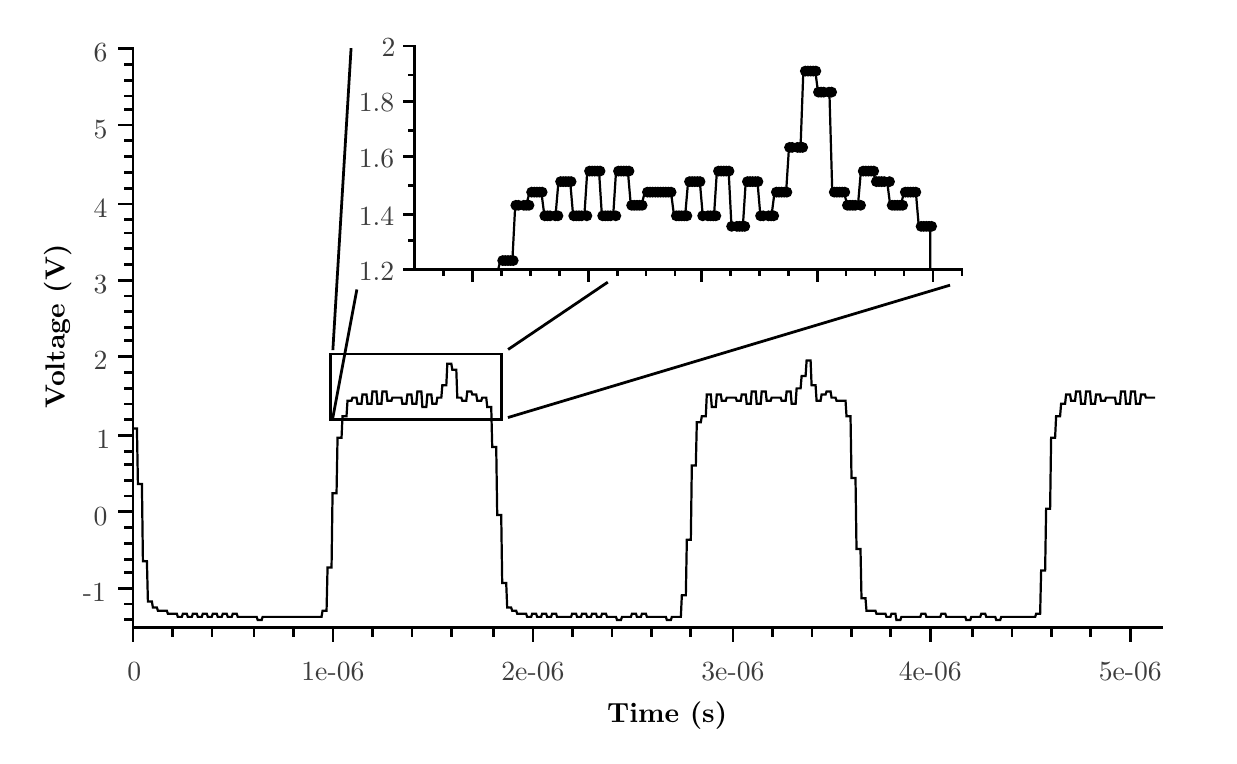
\begin{tikzpicture}{0pt}{0pt}{449pt}{269pt}
	\clip(0pt,269pt) -- (426.964pt,269pt) -- (426.964pt,13.2022pt) -- (0pt,13.2022pt) -- (0pt,269pt);
\begin{scope}
	\clip(139.785pt,262.344pt) -- (337.577pt,262.344pt) -- (337.577pt,181.515pt) -- (139.785pt,181.515pt) -- (139.785pt,262.344pt);
	\color[gray]{0}
	\draw[line width=0.8pt, line join=miter, line cap=rect](169.975pt,181.515pt) -- (171.016pt,185.557pt) -- (172.057pt,185.557pt) -- (173.098pt,185.557pt) -- (174.139pt,185.557pt) -- (175.18pt,185.557pt) -- (176.221pt,205.764pt) -- (177.262pt,205.764pt) -- (178.303pt,205.764pt) -- (179.344pt,205.764pt) -- (180.385pt,205.764pt) -- (181.426pt,209.805pt) -- (182.467pt,209.805pt) -- (183.508pt,209.805pt) -- (184.549pt,209.805pt) -- (185.59pt,209.805pt) -- (186.631pt,201.722pt) -- (187.672pt,201.722pt) -- (188.713pt,201.722pt) -- (189.754pt,201.722pt) -- (190.795pt,201.722pt) -- (191.836pt,213.847pt) -- (192.877pt,213.847pt) -- (193.918pt,213.847pt) -- (194.959pt,213.847pt) -- (196pt,213.847pt) -- (197.041pt,201.722pt) -- (198.082pt,201.722pt) -- (199.123pt,201.722pt) -- (200.164pt,201.722pt) -- (201.205pt,201.722pt) -- (202.246pt,217.888pt) -- (203.287pt,217.888pt) -- (204.328pt,217.888pt) -- (205.369pt,217.888pt) -- (206.41pt,217.888pt) -- (207.451pt,201.722pt) -- (208.492pt,201.722pt) -- (209.533pt,201.722pt) -- (210.574pt,201.722pt) -- (211.615pt,201.722pt) -- (212.656pt,217.888pt) -- (213.697pt,217.888pt) -- (214.738pt,217.888pt) -- (215.779pt,217.888pt) -- (216.82pt,217.888pt) -- (217.861pt,205.764pt) -- (218.902pt,205.764pt) -- (219.943pt,205.764pt) -- (220.984pt,205.764pt) -- (222.025pt,205.764pt) -- (223.066pt,209.805pt) -- (224.107pt,209.805pt) -- (225.148pt,209.805pt) -- (226.189pt,209.805pt) -- (227.23pt,209.805pt) -- (228.271pt,209.805pt) -- (229.312pt,209.805pt) -- (230.353pt,209.805pt) -- (231.394pt,209.805pt) -- (232.435pt,209.805pt) -- (233.476pt,201.722pt) -- (234.517pt,201.722pt) -- (235.558pt,201.722pt) -- (236.599pt,201.722pt) -- (237.64pt,201.722pt) -- (238.681pt,213.847pt) -- (239.722pt,213.847pt) -- (240.763pt,213.847pt) -- (241.804pt,213.847pt) -- (242.845pt,213.847pt) -- (243.886pt,201.722pt) -- (244.927pt,201.722pt) -- (245.968pt,201.722pt) -- (247.009pt,201.722pt) -- (248.05pt,201.722pt) -- (249.091pt,217.888pt) -- (250.132pt,217.888pt) -- (251.173pt,217.888pt) -- (252.214pt,217.888pt) -- (253.255pt,217.888pt) -- (254.296pt,197.681pt) -- (255.337pt,197.681pt) -- (256.378pt,197.681pt) -- (257.419pt,197.681pt) -- (258.46pt,197.681pt) -- (259.501pt,213.847pt) -- (260.542pt,213.847pt) -- (261.583pt,213.847pt) -- (262.624pt,213.847pt) -- (263.665pt,213.847pt) -- (264.706pt,201.722pt) -- (265.747pt,201.722pt) -- (266.788pt,201.722pt) -- (267.829pt,201.722pt) -- (268.87pt,201.722pt) -- (269.911pt,209.805pt) -- (270.952pt,209.805pt) -- (271.993pt,209.805pt) -- (273.034pt,209.805pt) -- (274.075pt,209.805pt) -- (275.116pt,225.971pt) -- (276.157pt,225.971pt) -- (277.198pt,225.971pt) -- (278.24pt,225.971pt) -- (279.281pt,225.971pt) -- (280.322pt,254.261pt) -- (281.363pt,254.261pt) -- (282.404pt,254.261pt) -- (283.445pt,254.261pt) -- (284.486pt,254.261pt) -- (285.527pt,246.178pt) -- (286.568pt,246.178pt) -- (287.609pt,246.178pt) -- (288.65pt,246.178pt) -- (289.691pt,246.178pt) -- (290.732pt,209.805pt) -- (291.773pt,209.805pt) -- (292.814pt,209.805pt) -- (293.855pt,209.805pt) -- (294.896pt,209.805pt) -- (295.937pt,205.764pt) -- (296.978pt,205.764pt) -- (298.019pt,205.764pt) -- (299.06pt,205.764pt) -- (300.101pt,205.764pt) -- (301.142pt,217.888pt) -- (302.183pt,217.888pt) -- (303.224pt,217.888pt) -- (304.265pt,217.888pt) -- (305.306pt,217.888pt) -- (306.347pt,213.847pt) -- (307.388pt,213.847pt) -- (308.429pt,213.847pt) -- (309.47pt,213.847pt) -- (310.511pt,213.847pt) -- (311.552pt,205.764pt) -- (312.593pt,205.764pt) -- (313.634pt,205.764pt) -- (314.675pt,205.764pt) -- (315.716pt,205.764pt) -- (316.757pt,209.805pt) -- (317.798pt,209.805pt) -- (318.839pt,209.805pt) -- (319.88pt,209.805pt) -- (320.921pt,209.805pt) -- (321.962pt,197.681pt) -- (323.003pt,197.681pt) -- (324.044pt,197.681pt) -- (325.085pt,197.681pt) -- (326.126pt,197.681pt) -- (326.126pt,181.515pt);
	\color[gray]{0}
	\fill(171.641pt,184.843pt) ellipse (1.42638pt and 1.42638pt);
	\draw[line width=1pt, line join=miter, line cap=rect](171.641pt,184.843pt) ellipse (1.42638pt and 1.42638pt);
	\fill(172.592pt,184.843pt) ellipse (1.42638pt and 1.42638pt);
	\draw[line width=1pt, line join=miter, line cap=rect](172.592pt,184.843pt) ellipse (1.42638pt and 1.42638pt);
	\fill(173.543pt,184.843pt) ellipse (1.42638pt and 1.42638pt);
	\draw[line width=1pt, line join=miter, line cap=rect](173.543pt,184.843pt) ellipse (1.42638pt and 1.42638pt);
	\fill(174.494pt,184.843pt) ellipse (1.42638pt and 1.42638pt);
	\draw[line width=1pt, line join=miter, line cap=rect](174.494pt,184.843pt) ellipse (1.42638pt and 1.42638pt);
	\fill(175.445pt,184.843pt) ellipse (1.42638pt and 1.42638pt);
	\draw[line width=1pt, line join=miter, line cap=rect](175.445pt,184.843pt) ellipse (1.42638pt and 1.42638pt);
	\fill(176.396pt,204.813pt) ellipse (1.42638pt and 1.42638pt);
	\draw[line width=1pt, line join=miter, line cap=rect](176.396pt,204.813pt) ellipse (1.42638pt and 1.42638pt);
	\fill(177.347pt,204.813pt) ellipse (1.42638pt and 1.42638pt);
	\draw[line width=1pt, line join=miter, line cap=rect](177.347pt,204.813pt) ellipse (1.42638pt and 1.42638pt);
	\fill(179.249pt,204.813pt) ellipse (1.42638pt and 1.42638pt);
	\draw[line width=1pt, line join=miter, line cap=rect](179.249pt,204.813pt) ellipse (1.42638pt and 1.42638pt);
	\fill(180.2pt,204.813pt) ellipse (1.42638pt and 1.42638pt);
	\draw[line width=1pt, line join=miter, line cap=rect](180.2pt,204.813pt) ellipse (1.42638pt and 1.42638pt);
	\fill(181.15pt,204.813pt) ellipse (1.42638pt and 1.42638pt);
	\draw[line width=1pt, line join=miter, line cap=rect](181.15pt,204.813pt) ellipse (1.42638pt and 1.42638pt);
	\fill(182.101pt,209.567pt) ellipse (1.42638pt and 1.42638pt);
	\draw[line width=1pt, line join=miter, line cap=rect](182.101pt,209.567pt) ellipse (1.42638pt and 1.42638pt);
	\fill(183.052pt,209.567pt) ellipse (1.42638pt and 1.42638pt);
	\draw[line width=1pt, line join=miter, line cap=rect](183.052pt,209.567pt) ellipse (1.42638pt and 1.42638pt);
	\fill(184.003pt,209.567pt) ellipse (1.42638pt and 1.42638pt);
	\draw[line width=1pt, line join=miter, line cap=rect](184.003pt,209.567pt) ellipse (1.42638pt and 1.42638pt);
	\fill(184.954pt,209.567pt) ellipse (1.42638pt and 1.42638pt);
	\draw[line width=1pt, line join=miter, line cap=rect](184.954pt,209.567pt) ellipse (1.42638pt and 1.42638pt);
	\fill(185.905pt,209.567pt) ellipse (1.42638pt and 1.42638pt);
	\draw[line width=1pt, line join=miter, line cap=rect](185.905pt,209.567pt) ellipse (1.42638pt and 1.42638pt);
	\fill(186.856pt,201.009pt) ellipse (1.42638pt and 1.42638pt);
	\draw[line width=1pt, line join=miter, line cap=rect](186.856pt,201.009pt) ellipse (1.42638pt and 1.42638pt);
	\fill(187.807pt,201.009pt) ellipse (1.42638pt and 1.42638pt);
	\draw[line width=1pt, line join=miter, line cap=rect](187.807pt,201.009pt) ellipse (1.42638pt and 1.42638pt);
	\fill(188.758pt,201.009pt) ellipse (1.42638pt and 1.42638pt);
	\draw[line width=1pt, line join=miter, line cap=rect](188.758pt,201.009pt) ellipse (1.42638pt and 1.42638pt);
	\fill(190.66pt,201.009pt) ellipse (1.42638pt and 1.42638pt);
	\draw[line width=1pt, line join=miter, line cap=rect](190.66pt,201.009pt) ellipse (1.42638pt and 1.42638pt);
	\fill(191.611pt,201.009pt) ellipse (1.42638pt and 1.42638pt);
	\draw[line width=1pt, line join=miter, line cap=rect](191.611pt,201.009pt) ellipse (1.42638pt and 1.42638pt);
	\fill(192.562pt,213.371pt) ellipse (1.42638pt and 1.42638pt);
	\draw[line width=1pt, line join=miter, line cap=rect](192.562pt,213.371pt) ellipse (1.42638pt and 1.42638pt);
	\fill(193.512pt,213.371pt) ellipse (1.42638pt and 1.42638pt);
	\draw[line width=1pt, line join=miter, line cap=rect](193.512pt,213.371pt) ellipse (1.42638pt and 1.42638pt);
	\fill(194.463pt,213.371pt) ellipse (1.42638pt and 1.42638pt);
	\draw[line width=1pt, line join=miter, line cap=rect](194.463pt,213.371pt) ellipse (1.42638pt and 1.42638pt);
	\fill(195.414pt,213.371pt) ellipse (1.42638pt and 1.42638pt);
	\draw[line width=1pt, line join=miter, line cap=rect](195.414pt,213.371pt) ellipse (1.42638pt and 1.42638pt);
	\fill(196.365pt,213.371pt) ellipse (1.42638pt and 1.42638pt);
	\draw[line width=1pt, line join=miter, line cap=rect](196.365pt,213.371pt) ellipse (1.42638pt and 1.42638pt);
	\fill(197.316pt,201.009pt) ellipse (1.42638pt and 1.42638pt);
	\draw[line width=1pt, line join=miter, line cap=rect](197.316pt,201.009pt) ellipse (1.42638pt and 1.42638pt);
	\fill(198.267pt,201.009pt) ellipse (1.42638pt and 1.42638pt);
	\draw[line width=1pt, line join=miter, line cap=rect](198.267pt,201.009pt) ellipse (1.42638pt and 1.42638pt);
	\fill(199.218pt,201.009pt) ellipse (1.42638pt and 1.42638pt);
	\draw[line width=1pt, line join=miter, line cap=rect](199.218pt,201.009pt) ellipse (1.42638pt and 1.42638pt);
	\fill(200.169pt,201.009pt) ellipse (1.42638pt and 1.42638pt);
	\draw[line width=1pt, line join=miter, line cap=rect](200.169pt,201.009pt) ellipse (1.42638pt and 1.42638pt);
	\fill(202.071pt,201.009pt) ellipse (1.42638pt and 1.42638pt);
	\draw[line width=1pt, line join=miter, line cap=rect](202.071pt,201.009pt) ellipse (1.42638pt and 1.42638pt);
	\fill(203.022pt,217.175pt) ellipse (1.42638pt and 1.42638pt);
	\draw[line width=1pt, line join=miter, line cap=rect](203.022pt,217.175pt) ellipse (1.42638pt and 1.42638pt);
	\fill(203.973pt,217.175pt) ellipse (1.42638pt and 1.42638pt);
	\draw[line width=1pt, line join=miter, line cap=rect](203.973pt,217.175pt) ellipse (1.42638pt and 1.42638pt);
	\fill(204.923pt,217.175pt) ellipse (1.42638pt and 1.42638pt);
	\draw[line width=1pt, line join=miter, line cap=rect](204.923pt,217.175pt) ellipse (1.42638pt and 1.42638pt);
	\fill(205.874pt,217.175pt) ellipse (1.42638pt and 1.42638pt);
	\draw[line width=1pt, line join=miter, line cap=rect](205.874pt,217.175pt) ellipse (1.42638pt and 1.42638pt);
	\fill(206.825pt,217.175pt) ellipse (1.42638pt and 1.42638pt);
	\draw[line width=1pt, line join=miter, line cap=rect](206.825pt,217.175pt) ellipse (1.42638pt and 1.42638pt);
	\fill(207.776pt,201.009pt) ellipse (1.42638pt and 1.42638pt);
	\draw[line width=1pt, line join=miter, line cap=rect](207.776pt,201.009pt) ellipse (1.42638pt and 1.42638pt);
	\fill(208.727pt,201.009pt) ellipse (1.42638pt and 1.42638pt);
	\draw[line width=1pt, line join=miter, line cap=rect](208.727pt,201.009pt) ellipse (1.42638pt and 1.42638pt);
	\fill(209.678pt,201.009pt) ellipse (1.42638pt and 1.42638pt);
	\draw[line width=1pt, line join=miter, line cap=rect](209.678pt,201.009pt) ellipse (1.42638pt and 1.42638pt);
	\fill(210.629pt,201.009pt) ellipse (1.42638pt and 1.42638pt);
	\draw[line width=1pt, line join=miter, line cap=rect](210.629pt,201.009pt) ellipse (1.42638pt and 1.42638pt);
	\fill(212.531pt,201.009pt) ellipse (1.42638pt and 1.42638pt);
	\draw[line width=1pt, line join=miter, line cap=rect](212.531pt,201.009pt) ellipse (1.42638pt and 1.42638pt);
	\fill(213.482pt,217.175pt) ellipse (1.42638pt and 1.42638pt);
	\draw[line width=1pt, line join=miter, line cap=rect](213.482pt,217.175pt) ellipse (1.42638pt and 1.42638pt);
	\fill(214.433pt,217.175pt) ellipse (1.42638pt and 1.42638pt);
	\draw[line width=1pt, line join=miter, line cap=rect](214.433pt,217.175pt) ellipse (1.42638pt and 1.42638pt);
	\fill(215.384pt,217.175pt) ellipse (1.42638pt and 1.42638pt);
	\draw[line width=1pt, line join=miter, line cap=rect](215.384pt,217.175pt) ellipse (1.42638pt and 1.42638pt);
	\fill(216.335pt,217.175pt) ellipse (1.42638pt and 1.42638pt);
	\draw[line width=1pt, line join=miter, line cap=rect](216.335pt,217.175pt) ellipse (1.42638pt and 1.42638pt);
	\fill(217.285pt,217.175pt) ellipse (1.42638pt and 1.42638pt);
	\draw[line width=1pt, line join=miter, line cap=rect](217.285pt,217.175pt) ellipse (1.42638pt and 1.42638pt);
	\fill(218.236pt,204.813pt) ellipse (1.42638pt and 1.42638pt);
	\draw[line width=1pt, line join=miter, line cap=rect](218.236pt,204.813pt) ellipse (1.42638pt and 1.42638pt);
	\fill(219.187pt,204.813pt) ellipse (1.42638pt and 1.42638pt);
	\draw[line width=1pt, line join=miter, line cap=rect](219.187pt,204.813pt) ellipse (1.42638pt and 1.42638pt);
	\fill(220.138pt,204.813pt) ellipse (1.42638pt and 1.42638pt);
	\draw[line width=1pt, line join=miter, line cap=rect](220.138pt,204.813pt) ellipse (1.42638pt and 1.42638pt);
	\fill(221.089pt,204.813pt) ellipse (1.42638pt and 1.42638pt);
	\draw[line width=1pt, line join=miter, line cap=rect](221.089pt,204.813pt) ellipse (1.42638pt and 1.42638pt);
	\fill(222.04pt,204.813pt) ellipse (1.42638pt and 1.42638pt);
	\draw[line width=1pt, line join=miter, line cap=rect](222.04pt,204.813pt) ellipse (1.42638pt and 1.42638pt);
	\fill(223.942pt,209.567pt) ellipse (1.42638pt and 1.42638pt);
	\draw[line width=1pt, line join=miter, line cap=rect](223.942pt,209.567pt) ellipse (1.42638pt and 1.42638pt);
	\fill(224.893pt,209.567pt) ellipse (1.42638pt and 1.42638pt);
	\draw[line width=1pt, line join=miter, line cap=rect](224.893pt,209.567pt) ellipse (1.42638pt and 1.42638pt);
	\fill(225.844pt,209.567pt) ellipse (1.42638pt and 1.42638pt);
	\draw[line width=1pt, line join=miter, line cap=rect](225.844pt,209.567pt) ellipse (1.42638pt and 1.42638pt);
	\fill(226.795pt,209.567pt) ellipse (1.42638pt and 1.42638pt);
	\draw[line width=1pt, line join=miter, line cap=rect](226.795pt,209.567pt) ellipse (1.42638pt and 1.42638pt);
	\fill(227.746pt,209.567pt) ellipse (1.42638pt and 1.42638pt);
	\draw[line width=1pt, line join=miter, line cap=rect](227.746pt,209.567pt) ellipse (1.42638pt and 1.42638pt);
	\fill(228.697pt,209.567pt) ellipse (1.42638pt and 1.42638pt);
	\draw[line width=1pt, line join=miter, line cap=rect](228.697pt,209.567pt) ellipse (1.42638pt and 1.42638pt);
	\fill(229.647pt,209.567pt) ellipse (1.42638pt and 1.42638pt);
	\draw[line width=1pt, line join=miter, line cap=rect](229.647pt,209.567pt) ellipse (1.42638pt and 1.42638pt);
	\fill(230.598pt,209.567pt) ellipse (1.42638pt and 1.42638pt);
	\draw[line width=1pt, line join=miter, line cap=rect](230.598pt,209.567pt) ellipse (1.42638pt and 1.42638pt);
	\fill(231.549pt,209.567pt) ellipse (1.42638pt and 1.42638pt);
	\draw[line width=1pt, line join=miter, line cap=rect](231.549pt,209.567pt) ellipse (1.42638pt and 1.42638pt);
	\fill(232.5pt,209.567pt) ellipse (1.42638pt and 1.42638pt);
	\draw[line width=1pt, line join=miter, line cap=rect](232.5pt,209.567pt) ellipse (1.42638pt and 1.42638pt);
	\fill(234.402pt,201.009pt) ellipse (1.42638pt and 1.42638pt);
	\draw[line width=1pt, line join=miter, line cap=rect](234.402pt,201.009pt) ellipse (1.42638pt and 1.42638pt);
	\fill(235.353pt,201.009pt) ellipse (1.42638pt and 1.42638pt);
	\draw[line width=1pt, line join=miter, line cap=rect](235.353pt,201.009pt) ellipse (1.42638pt and 1.42638pt);
	\fill(236.304pt,201.009pt) ellipse (1.42638pt and 1.42638pt);
	\draw[line width=1pt, line join=miter, line cap=rect](236.304pt,201.009pt) ellipse (1.42638pt and 1.42638pt);
	\fill(237.255pt,201.009pt) ellipse (1.42638pt and 1.42638pt);
	\draw[line width=1pt, line join=miter, line cap=rect](237.255pt,201.009pt) ellipse (1.42638pt and 1.42638pt);
	\fill(238.206pt,201.009pt) ellipse (1.42638pt and 1.42638pt);
	\draw[line width=1pt, line join=miter, line cap=rect](238.206pt,201.009pt) ellipse (1.42638pt and 1.42638pt);
	\fill(239.157pt,213.371pt) ellipse (1.42638pt and 1.42638pt);
	\draw[line width=1pt, line join=miter, line cap=rect](239.157pt,213.371pt) ellipse (1.42638pt and 1.42638pt);
	\fill(240.108pt,213.371pt) ellipse (1.42638pt and 1.42638pt);
	\draw[line width=1pt, line join=miter, line cap=rect](240.108pt,213.371pt) ellipse (1.42638pt and 1.42638pt);
	\fill(241.058pt,213.371pt) ellipse (1.42638pt and 1.42638pt);
	\draw[line width=1pt, line join=miter, line cap=rect](241.058pt,213.371pt) ellipse (1.42638pt and 1.42638pt);
	\fill(242.009pt,213.371pt) ellipse (1.42638pt and 1.42638pt);
	\draw[line width=1pt, line join=miter, line cap=rect](242.009pt,213.371pt) ellipse (1.42638pt and 1.42638pt);
	\fill(242.96pt,213.371pt) ellipse (1.42638pt and 1.42638pt);
	\draw[line width=1pt, line join=miter, line cap=rect](242.96pt,213.371pt) ellipse (1.42638pt and 1.42638pt);
	\fill(243.911pt,201.009pt) ellipse (1.42638pt and 1.42638pt);
	\draw[line width=1pt, line join=miter, line cap=rect](243.911pt,201.009pt) ellipse (1.42638pt and 1.42638pt);
	\fill(245.813pt,201.009pt) ellipse (1.42638pt and 1.42638pt);
	\draw[line width=1pt, line join=miter, line cap=rect](245.813pt,201.009pt) ellipse (1.42638pt and 1.42638pt);
	\fill(246.764pt,201.009pt) ellipse (1.42638pt and 1.42638pt);
	\draw[line width=1pt, line join=miter, line cap=rect](246.764pt,201.009pt) ellipse (1.42638pt and 1.42638pt);
	\fill(247.715pt,201.009pt) ellipse (1.42638pt and 1.42638pt);
	\draw[line width=1pt, line join=miter, line cap=rect](247.715pt,201.009pt) ellipse (1.42638pt and 1.42638pt);
	\fill(248.666pt,201.009pt) ellipse (1.42638pt and 1.42638pt);
	\draw[line width=1pt, line join=miter, line cap=rect](248.666pt,201.009pt) ellipse (1.42638pt and 1.42638pt);
	\fill(249.617pt,217.175pt) ellipse (1.42638pt and 1.42638pt);
	\draw[line width=1pt, line join=miter, line cap=rect](249.617pt,217.175pt) ellipse (1.42638pt and 1.42638pt);
	\fill(250.568pt,217.175pt) ellipse (1.42638pt and 1.42638pt);
	\draw[line width=1pt, line join=miter, line cap=rect](250.568pt,217.175pt) ellipse (1.42638pt and 1.42638pt);
	\fill(251.519pt,217.175pt) ellipse (1.42638pt and 1.42638pt);
	\draw[line width=1pt, line join=miter, line cap=rect](251.519pt,217.175pt) ellipse (1.42638pt and 1.42638pt);
	\fill(252.47pt,217.175pt) ellipse (1.42638pt and 1.42638pt);
	\draw[line width=1pt, line join=miter, line cap=rect](252.47pt,217.175pt) ellipse (1.42638pt and 1.42638pt);
	\fill(253.42pt,217.175pt) ellipse (1.42638pt and 1.42638pt);
	\draw[line width=1pt, line join=miter, line cap=rect](253.42pt,217.175pt) ellipse (1.42638pt and 1.42638pt);
	\fill(254.371pt,197.205pt) ellipse (1.42638pt and 1.42638pt);
	\draw[line width=1pt, line join=miter, line cap=rect](254.371pt,197.205pt) ellipse (1.42638pt and 1.42638pt);
	\fill(256.273pt,197.205pt) ellipse (1.42638pt and 1.42638pt);
	\draw[line width=1pt, line join=miter, line cap=rect](256.273pt,197.205pt) ellipse (1.42638pt and 1.42638pt);
	\fill(257.224pt,197.205pt) ellipse (1.42638pt and 1.42638pt);
	\draw[line width=1pt, line join=miter, line cap=rect](257.224pt,197.205pt) ellipse (1.42638pt and 1.42638pt);
	\fill(258.175pt,197.205pt) ellipse (1.42638pt and 1.42638pt);
	\draw[line width=1pt, line join=miter, line cap=rect](258.175pt,197.205pt) ellipse (1.42638pt and 1.42638pt);
	\fill(259.126pt,197.205pt) ellipse (1.42638pt and 1.42638pt);
	\draw[line width=1pt, line join=miter, line cap=rect](259.126pt,197.205pt) ellipse (1.42638pt and 1.42638pt);
	\fill(260.077pt,213.371pt) ellipse (1.42638pt and 1.42638pt);
	\draw[line width=1pt, line join=miter, line cap=rect](260.077pt,213.371pt) ellipse (1.42638pt and 1.42638pt);
	\fill(261.028pt,213.371pt) ellipse (1.42638pt and 1.42638pt);
	\draw[line width=1pt, line join=miter, line cap=rect](261.028pt,213.371pt) ellipse (1.42638pt and 1.42638pt);
	\fill(261.979pt,213.371pt) ellipse (1.42638pt and 1.42638pt);
	\draw[line width=1pt, line join=miter, line cap=rect](261.979pt,213.371pt) ellipse (1.42638pt and 1.42638pt);
	\fill(262.93pt,213.371pt) ellipse (1.42638pt and 1.42638pt);
	\draw[line width=1pt, line join=miter, line cap=rect](262.93pt,213.371pt) ellipse (1.42638pt and 1.42638pt);
	\fill(263.881pt,213.371pt) ellipse (1.42638pt and 1.42638pt);
	\draw[line width=1pt, line join=miter, line cap=rect](263.881pt,213.371pt) ellipse (1.42638pt and 1.42638pt);
	\fill(264.832pt,201.009pt) ellipse (1.42638pt and 1.42638pt);
	\draw[line width=1pt, line join=miter, line cap=rect](264.832pt,201.009pt) ellipse (1.42638pt and 1.42638pt);
	\fill(265.782pt,201.009pt) ellipse (1.42638pt and 1.42638pt);
	\draw[line width=1pt, line join=miter, line cap=rect](265.782pt,201.009pt) ellipse (1.42638pt and 1.42638pt);
	\fill(267.684pt,201.009pt) ellipse (1.42638pt and 1.42638pt);
	\draw[line width=1pt, line join=miter, line cap=rect](267.684pt,201.009pt) ellipse (1.42638pt and 1.42638pt);
	\fill(268.635pt,201.009pt) ellipse (1.42638pt and 1.42638pt);
	\draw[line width=1pt, line join=miter, line cap=rect](268.635pt,201.009pt) ellipse (1.42638pt and 1.42638pt);
	\fill(269.586pt,201.009pt) ellipse (1.42638pt and 1.42638pt);
	\draw[line width=1pt, line join=miter, line cap=rect](269.586pt,201.009pt) ellipse (1.42638pt and 1.42638pt);
	\fill(270.537pt,209.567pt) ellipse (1.42638pt and 1.42638pt);
	\draw[line width=1pt, line join=miter, line cap=rect](270.537pt,209.567pt) ellipse (1.42638pt and 1.42638pt);
	\fill(271.488pt,209.567pt) ellipse (1.42638pt and 1.42638pt);
	\draw[line width=1pt, line join=miter, line cap=rect](271.488pt,209.567pt) ellipse (1.42638pt and 1.42638pt);
	\fill(272.439pt,209.567pt) ellipse (1.42638pt and 1.42638pt);
	\draw[line width=1pt, line join=miter, line cap=rect](272.439pt,209.567pt) ellipse (1.42638pt and 1.42638pt);
	\fill(273.39pt,209.567pt) ellipse (1.42638pt and 1.42638pt);
	\draw[line width=1pt, line join=miter, line cap=rect](273.39pt,209.567pt) ellipse (1.42638pt and 1.42638pt);
	\fill(274.341pt,209.567pt) ellipse (1.42638pt and 1.42638pt);
	\draw[line width=1pt, line join=miter, line cap=rect](274.341pt,209.567pt) ellipse (1.42638pt and 1.42638pt);
	\fill(275.292pt,225.733pt) ellipse (1.42638pt and 1.42638pt);
	\draw[line width=1pt, line join=miter, line cap=rect](275.292pt,225.733pt) ellipse (1.42638pt and 1.42638pt);
	\fill(276.243pt,225.733pt) ellipse (1.42638pt and 1.42638pt);
	\draw[line width=1pt, line join=miter, line cap=rect](276.243pt,225.733pt) ellipse (1.42638pt and 1.42638pt);
	\fill(278.144pt,225.733pt) ellipse (1.42638pt and 1.42638pt);
	\draw[line width=1pt, line join=miter, line cap=rect](278.144pt,225.733pt) ellipse (1.42638pt and 1.42638pt);
	\fill(279.095pt,225.733pt) ellipse (1.42638pt and 1.42638pt);
	\draw[line width=1pt, line join=miter, line cap=rect](279.095pt,225.733pt) ellipse (1.42638pt and 1.42638pt);
	\fill(280.046pt,225.733pt) ellipse (1.42638pt and 1.42638pt);
	\draw[line width=1pt, line join=miter, line cap=rect](280.046pt,225.733pt) ellipse (1.42638pt and 1.42638pt);
	\fill(280.997pt,253.31pt) ellipse (1.42638pt and 1.42638pt);
	\draw[line width=1pt, line join=miter, line cap=rect](280.997pt,253.31pt) ellipse (1.42638pt and 1.42638pt);
	\fill(281.948pt,253.31pt) ellipse (1.42638pt and 1.42638pt);
	\draw[line width=1pt, line join=miter, line cap=rect](281.948pt,253.31pt) ellipse (1.42638pt and 1.42638pt);
	\fill(282.899pt,253.31pt) ellipse (1.42638pt and 1.42638pt);
	\draw[line width=1pt, line join=miter, line cap=rect](282.899pt,253.31pt) ellipse (1.42638pt and 1.42638pt);
	\fill(283.85pt,253.31pt) ellipse (1.42638pt and 1.42638pt);
	\draw[line width=1pt, line join=miter, line cap=rect](283.85pt,253.31pt) ellipse (1.42638pt and 1.42638pt);
	\fill(284.801pt,253.31pt) ellipse (1.42638pt and 1.42638pt);
	\draw[line width=1pt, line join=miter, line cap=rect](284.801pt,253.31pt) ellipse (1.42638pt and 1.42638pt);
	\fill(285.752pt,245.702pt) ellipse (1.42638pt and 1.42638pt);
	\draw[line width=1pt, line join=miter, line cap=rect](285.752pt,245.702pt) ellipse (1.42638pt and 1.42638pt);
	\fill(286.703pt,245.702pt) ellipse (1.42638pt and 1.42638pt);
	\draw[line width=1pt, line join=miter, line cap=rect](286.703pt,245.702pt) ellipse (1.42638pt and 1.42638pt);
	\fill(287.654pt,245.702pt) ellipse (1.42638pt and 1.42638pt);
	\draw[line width=1pt, line join=miter, line cap=rect](287.654pt,245.702pt) ellipse (1.42638pt and 1.42638pt);
	\fill(289.555pt,245.702pt) ellipse (1.42638pt and 1.42638pt);
	\draw[line width=1pt, line join=miter, line cap=rect](289.555pt,245.702pt) ellipse (1.42638pt and 1.42638pt);
	\fill(290.506pt,245.702pt) ellipse (1.42638pt and 1.42638pt);
	\draw[line width=1pt, line join=miter, line cap=rect](290.506pt,245.702pt) ellipse (1.42638pt and 1.42638pt);
	\fill(291.457pt,209.567pt) ellipse (1.42638pt and 1.42638pt);
	\draw[line width=1pt, line join=miter, line cap=rect](291.457pt,209.567pt) ellipse (1.42638pt and 1.42638pt);
	\fill(292.408pt,209.567pt) ellipse (1.42638pt and 1.42638pt);
	\draw[line width=1pt, line join=miter, line cap=rect](292.408pt,209.567pt) ellipse (1.42638pt and 1.42638pt);
	\fill(293.359pt,209.567pt) ellipse (1.42638pt and 1.42638pt);
	\draw[line width=1pt, line join=miter, line cap=rect](293.359pt,209.567pt) ellipse (1.42638pt and 1.42638pt);
	\fill(294.31pt,209.567pt) ellipse (1.42638pt and 1.42638pt);
	\draw[line width=1pt, line join=miter, line cap=rect](294.31pt,209.567pt) ellipse (1.42638pt and 1.42638pt);
	\fill(295.261pt,209.567pt) ellipse (1.42638pt and 1.42638pt);
	\draw[line width=1pt, line join=miter, line cap=rect](295.261pt,209.567pt) ellipse (1.42638pt and 1.42638pt);
	\fill(296.212pt,204.813pt) ellipse (1.42638pt and 1.42638pt);
	\draw[line width=1pt, line join=miter, line cap=rect](296.212pt,204.813pt) ellipse (1.42638pt and 1.42638pt);
	\fill(297.163pt,204.813pt) ellipse (1.42638pt and 1.42638pt);
	\draw[line width=1pt, line join=miter, line cap=rect](297.163pt,204.813pt) ellipse (1.42638pt and 1.42638pt);
	\fill(298.114pt,204.813pt) ellipse (1.42638pt and 1.42638pt);
	\draw[line width=1pt, line join=miter, line cap=rect](298.114pt,204.813pt) ellipse (1.42638pt and 1.42638pt);
	\fill(299.065pt,204.813pt) ellipse (1.42638pt and 1.42638pt);
	\draw[line width=1pt, line join=miter, line cap=rect](299.065pt,204.813pt) ellipse (1.42638pt and 1.42638pt);
	\fill(300.967pt,204.813pt) ellipse (1.42638pt and 1.42638pt);
	\draw[line width=1pt, line join=miter, line cap=rect](300.967pt,204.813pt) ellipse (1.42638pt and 1.42638pt);
	\fill(301.917pt,217.175pt) ellipse (1.42638pt and 1.42638pt);
	\draw[line width=1pt, line join=miter, line cap=rect](301.917pt,217.175pt) ellipse (1.42638pt and 1.42638pt);
	\fill(302.868pt,217.175pt) ellipse (1.42638pt and 1.42638pt);
	\draw[line width=1pt, line join=miter, line cap=rect](302.868pt,217.175pt) ellipse (1.42638pt and 1.42638pt);
	\fill(303.819pt,217.175pt) ellipse (1.42638pt and 1.42638pt);
	\draw[line width=1pt, line join=miter, line cap=rect](303.819pt,217.175pt) ellipse (1.42638pt and 1.42638pt);
	\fill(304.77pt,217.175pt) ellipse (1.42638pt and 1.42638pt);
	\draw[line width=1pt, line join=miter, line cap=rect](304.77pt,217.175pt) ellipse (1.42638pt and 1.42638pt);
	\fill(305.721pt,217.175pt) ellipse (1.42638pt and 1.42638pt);
	\draw[line width=1pt, line join=miter, line cap=rect](305.721pt,217.175pt) ellipse (1.42638pt and 1.42638pt);
	\fill(306.672pt,213.371pt) ellipse (1.42638pt and 1.42638pt);
	\draw[line width=1pt, line join=miter, line cap=rect](306.672pt,213.371pt) ellipse (1.42638pt and 1.42638pt);
	\fill(307.623pt,213.371pt) ellipse (1.42638pt and 1.42638pt);
	\draw[line width=1pt, line join=miter, line cap=rect](307.623pt,213.371pt) ellipse (1.42638pt and 1.42638pt);
	\fill(308.574pt,213.371pt) ellipse (1.42638pt and 1.42638pt);
	\draw[line width=1pt, line join=miter, line cap=rect](308.574pt,213.371pt) ellipse (1.42638pt and 1.42638pt);
	\fill(309.525pt,213.371pt) ellipse (1.42638pt and 1.42638pt);
	\draw[line width=1pt, line join=miter, line cap=rect](309.525pt,213.371pt) ellipse (1.42638pt and 1.42638pt);
	\fill(311.427pt,213.371pt) ellipse (1.42638pt and 1.42638pt);
	\draw[line width=1pt, line join=miter, line cap=rect](311.427pt,213.371pt) ellipse (1.42638pt and 1.42638pt);
	\fill(312.378pt,204.813pt) ellipse (1.42638pt and 1.42638pt);
	\draw[line width=1pt, line join=miter, line cap=rect](312.378pt,204.813pt) ellipse (1.42638pt and 1.42638pt);
	\fill(313.328pt,204.813pt) ellipse (1.42638pt and 1.42638pt);
	\draw[line width=1pt, line join=miter, line cap=rect](313.328pt,204.813pt) ellipse (1.42638pt and 1.42638pt);
	\fill(314.279pt,204.813pt) ellipse (1.42638pt and 1.42638pt);
	\draw[line width=1pt, line join=miter, line cap=rect](314.279pt,204.813pt) ellipse (1.42638pt and 1.42638pt);
	\fill(315.23pt,204.813pt) ellipse (1.42638pt and 1.42638pt);
	\draw[line width=1pt, line join=miter, line cap=rect](315.23pt,204.813pt) ellipse (1.42638pt and 1.42638pt);
	\fill(316.181pt,204.813pt) ellipse (1.42638pt and 1.42638pt);
	\draw[line width=1pt, line join=miter, line cap=rect](316.181pt,204.813pt) ellipse (1.42638pt and 1.42638pt);
	\fill(317.132pt,209.567pt) ellipse (1.42638pt and 1.42638pt);
	\draw[line width=1pt, line join=miter, line cap=rect](317.132pt,209.567pt) ellipse (1.42638pt and 1.42638pt);
	\fill(318.083pt,209.567pt) ellipse (1.42638pt and 1.42638pt);
	\draw[line width=1pt, line join=miter, line cap=rect](318.083pt,209.567pt) ellipse (1.42638pt and 1.42638pt);
	\fill(319.034pt,209.567pt) ellipse (1.42638pt and 1.42638pt);
	\draw[line width=1pt, line join=miter, line cap=rect](319.034pt,209.567pt) ellipse (1.42638pt and 1.42638pt);
	\fill(319.985pt,209.567pt) ellipse (1.42638pt and 1.42638pt);
	\draw[line width=1pt, line join=miter, line cap=rect](319.985pt,209.567pt) ellipse (1.42638pt and 1.42638pt);
	\fill(320.936pt,209.567pt) ellipse (1.42638pt and 1.42638pt);
	\draw[line width=1pt, line join=miter, line cap=rect](320.936pt,209.567pt) ellipse (1.42638pt and 1.42638pt);
	\fill(322.838pt,197.205pt) ellipse (1.42638pt and 1.42638pt);
	\draw[line width=1pt, line join=miter, line cap=rect](322.838pt,197.205pt) ellipse (1.42638pt and 1.42638pt);
	\fill(323.789pt,197.205pt) ellipse (1.42638pt and 1.42638pt);
	\draw[line width=1pt, line join=miter, line cap=rect](323.789pt,197.205pt) ellipse (1.42638pt and 1.42638pt);
	\fill(324.74pt,197.205pt) ellipse (1.42638pt and 1.42638pt);
	\draw[line width=1pt, line join=miter, line cap=rect](324.74pt,197.205pt) ellipse (1.42638pt and 1.42638pt);
	\fill(325.69pt,197.205pt) ellipse (1.42638pt and 1.42638pt);
	\draw[line width=1pt, line join=miter, line cap=rect](325.69pt,197.205pt) ellipse (1.42638pt and 1.42638pt);
	\fill(326.641pt,197.205pt) ellipse (1.42638pt and 1.42638pt);
	\draw[line width=1pt, line join=miter, line cap=rect](326.641pt,197.205pt) ellipse (1.42638pt and 1.42638pt);
\end{scope}
\begin{scope}
	\color[gray]{0.235294}
	\pgftext[center, base, at={\pgfpoint{126.049pt}{177.712pt}}]{1.2}
	\pgftext[center, base, at={\pgfpoint{126.049pt}{197.681pt}}]{1.4}
	\pgftext[center, base, at={\pgfpoint{126.049pt}{218.601pt}}]{1.6}
	\pgftext[center, base, at={\pgfpoint{126.049pt}{238.571pt}}]{1.8}
	\pgftext[center, base, at={\pgfpoint{130.373pt}{258.54pt}}]{2}
	\color[gray]{0}
	\draw[line width=1pt, line join=bevel, line cap=rect](139.785pt,191.975pt) -- (137.884pt,191.975pt);
	\draw[line width=1pt, line join=bevel, line cap=rect](139.785pt,211.945pt) -- (137.884pt,211.945pt);
	\draw[line width=1pt, line join=bevel, line cap=rect](139.785pt,231.914pt) -- (137.884pt,231.914pt);
	\draw[line width=1pt, line join=bevel, line cap=rect](139.785pt,251.883pt) -- (137.884pt,251.883pt);
	\draw[line width=1pt, line join=bevel, line cap=rect](139.785pt,181.515pt) -- (135.982pt,181.515pt);
	\draw[line width=1pt, line join=bevel, line cap=rect](139.785pt,201.485pt) -- (135.982pt,201.485pt);
	\draw[line width=1pt, line join=bevel, line cap=rect](139.785pt,222.405pt) -- (135.982pt,222.405pt);
	\draw[line width=1pt, line join=bevel, line cap=rect](139.785pt,242.374pt) -- (135.982pt,242.374pt);
	\draw[line width=1pt, line join=bevel, line cap=rect](139.785pt,262.344pt) -- (135.982pt,262.344pt);
	\draw[line width=1pt, line join=bevel, line cap=rect](139.785pt,262.344pt) -- (139.785pt,181.515pt);
	\draw[line width=1pt, line join=bevel, line cap=rect](150.246pt,181.515pt) -- (150.246pt,179.613pt);
	\draw[line width=1pt, line join=bevel, line cap=rect](171.166pt,181.515pt) -- (171.166pt,179.613pt);
	\draw[line width=1pt, line join=bevel, line cap=rect](192.086pt,181.515pt) -- (192.086pt,179.613pt);
	\draw[line width=1pt, line join=bevel, line cap=rect](213.006pt,181.515pt) -- (213.006pt,179.613pt);
	\draw[line width=1pt, line join=bevel, line cap=rect](233.927pt,181.515pt) -- (233.927pt,179.613pt);
	\draw[line width=1pt, line join=bevel, line cap=rect](253.896pt,181.515pt) -- (253.896pt,179.613pt);
	\draw[line width=1pt, line join=bevel, line cap=rect](274.816pt,181.515pt) -- (274.816pt,179.613pt);
	\draw[line width=1pt, line join=bevel, line cap=rect](295.736pt,181.515pt) -- (295.736pt,179.613pt);
	\draw[line width=1pt, line join=bevel, line cap=rect](316.657pt,181.515pt) -- (316.657pt,179.613pt);
	\draw[line width=1pt, line join=bevel, line cap=rect](337.577pt,181.515pt) -- (337.577pt,179.613pt);
	\draw[line width=1pt, line join=bevel, line cap=rect](181.626pt,181.515pt) -- (181.626pt,179.613pt);
	\draw[line width=1pt, line join=bevel, line cap=rect](223.466pt,181.515pt) -- (223.466pt,179.613pt);
	\draw[line width=1pt, line join=bevel, line cap=rect](264.356pt,181.515pt) -- (264.356pt,179.613pt);
	\draw[line width=1pt, line join=bevel, line cap=rect](306.197pt,181.515pt) -- (306.197pt,179.613pt);
	\draw[line width=1pt, line join=bevel, line cap=rect](160.706pt,181.515pt) -- (160.706pt,177.712pt);
	\draw[line width=1pt, line join=bevel, line cap=rect](202.546pt,181.515pt) -- (202.546pt,177.712pt);
	\draw[line width=1pt, line join=bevel, line cap=rect](243.436pt,181.515pt) -- (243.436pt,177.712pt);
	\draw[line width=1pt, line join=bevel, line cap=rect](285.276pt,181.515pt) -- (285.276pt,177.712pt);
	\draw[line width=1pt, line join=bevel, line cap=rect](327.117pt,181.515pt) -- (327.117pt,177.712pt);
	\draw[line width=1pt, line join=bevel, line cap=rect](139.785pt,181.515pt) -- (337.577pt,181.515pt);
\end{scope}
\begin{scope}
	\clip(38.0368pt,261.393pt) -- (409.847pt,261.393pt) -- (409.847pt,52.19pt) -- (38.0368pt,52.19pt) -- (38.0368pt,261.393pt);
	\color[gray]{0}
	\draw[line width=0.8pt, line join=miter, line cap=rect](38.3975pt,124.156pt) -- (38.7581pt,124.156pt) -- (39.1187pt,124.156pt) -- (39.4794pt,124.156pt) -- (39.84pt,104.072pt) -- (40.2006pt,104.072pt) -- (40.5613pt,104.072pt) -- (40.9219pt,104.072pt) -- (41.2825pt,104.072pt) -- (41.6431pt,76.1786pt) -- (42.0038pt,76.1786pt) -- (42.3644pt,76.1786pt) -- (42.725pt,76.1786pt) -- (43.0857pt,76.1786pt) -- (43.4463pt,61.6739pt) -- (43.8069pt,61.6739pt) -- (44.1676pt,61.6739pt) -- (44.5282pt,61.6739pt) -- (44.8888pt,61.6739pt) -- (45.2495pt,59.4424pt) -- (45.6101pt,59.4424pt) -- (45.9707pt,59.4424pt) -- (46.3313pt,59.4424pt) -- (46.692pt,59.4424pt) -- (47.0526pt,58.3266pt) -- (47.4132pt,58.3266pt) -- (47.7739pt,58.3266pt) -- (48.1345pt,58.3266pt) -- (48.4951pt,58.3266pt) -- (48.8558pt,58.3266pt) -- (49.2164pt,58.3266pt) -- (49.577pt,58.3266pt) -- (49.9377pt,58.3266pt) -- (50.2983pt,58.3266pt) -- (50.6589pt,57.2109pt) -- (51.0195pt,57.2109pt) -- (51.3802pt,57.2109pt) -- (51.7408pt,57.2109pt) -- (52.1014pt,57.2109pt) -- (52.4621pt,57.2109pt) -- (52.8227pt,57.2109pt) -- (53.1833pt,57.2109pt) -- (53.544pt,57.2109pt) -- (53.9046pt,57.2109pt) -- (54.2652pt,56.0951pt) -- (54.6258pt,56.0951pt) -- (54.9865pt,56.0951pt) -- (55.3471pt,56.0951pt) -- (55.7077pt,56.0951pt) -- (56.0684pt,57.2109pt) -- (56.429pt,57.2109pt) -- (56.7896pt,57.2109pt) -- (57.1503pt,57.2109pt) -- (57.5109pt,57.2109pt) -- (57.8715pt,56.0951pt) -- (58.2322pt,56.0951pt) -- (58.5928pt,56.0951pt) -- (58.9534pt,56.0951pt) -- (59.314pt,56.0951pt) -- (59.6747pt,57.2109pt) -- (60.0353pt,57.2109pt) -- (60.3959pt,57.2109pt) -- (60.7566pt,57.2109pt) -- (61.1172pt,57.2109pt) -- (61.4778pt,56.0951pt) -- (61.8385pt,56.0951pt) -- (62.1991pt,56.0951pt) -- (62.5597pt,56.0951pt) -- (62.9204pt,56.0951pt) -- (63.281pt,57.2109pt) -- (63.6416pt,57.2109pt) -- (64.0022pt,57.2109pt) -- (64.3629pt,57.2109pt) -- (64.7235pt,57.2109pt) -- (65.0841pt,56.0951pt) -- (65.4448pt,56.0951pt) -- (65.8054pt,56.0951pt) -- (66.166pt,56.0951pt) -- (66.5267pt,56.0951pt) -- (66.8873pt,57.2109pt) -- (67.2479pt,57.2109pt) -- (67.6085pt,57.2109pt) -- (67.9692pt,57.2109pt) -- (68.3298pt,57.2109pt) -- (68.6904pt,56.0951pt) -- (69.0511pt,56.0951pt) -- (69.4117pt,56.0951pt) -- (69.7723pt,56.0951pt) -- (70.133pt,56.0951pt) -- (70.4936pt,57.2109pt) -- (70.8542pt,57.2109pt) -- (71.2149pt,57.2109pt) -- (71.5755pt,57.2109pt) -- (71.9361pt,57.2109pt) -- (72.2967pt,56.0951pt) -- (72.6574pt,56.0951pt) -- (73.018pt,56.0951pt) -- (73.3786pt,56.0951pt) -- (73.7393pt,56.0951pt) -- (74.0999pt,57.2109pt) -- (74.4605pt,57.2109pt) -- (74.8212pt,57.2109pt) -- (75.1818pt,57.2109pt) -- (75.5424pt,57.2109pt) -- (75.9031pt,56.0951pt) -- (76.2637pt,56.0951pt) -- (76.6243pt,56.0951pt) -- (76.9849pt,56.0951pt) -- (77.3456pt,56.0951pt) -- (77.7062pt,56.0951pt) -- (78.0668pt,56.0951pt) -- (78.4275pt,56.0951pt) -- (78.7881pt,56.0951pt) -- (79.1487pt,56.0951pt) -- (79.5094pt,56.0951pt) -- (79.87pt,56.0951pt) -- (80.2306pt,56.0951pt) -- (80.5913pt,56.0951pt) -- (80.9519pt,56.0951pt) -- (81.3125pt,56.0951pt) -- (81.6731pt,56.0951pt) -- (82.0338pt,56.0951pt) -- (82.3944pt,56.0951pt) -- (82.755pt,56.0951pt) -- (83.1157pt,54.9794pt) -- (83.4763pt,54.9794pt) -- (83.8369pt,54.9794pt) -- (84.1976pt,54.9794pt) -- (84.5582pt,54.9794pt) -- (84.9188pt,56.0951pt) -- (85.2794pt,56.0951pt) -- (85.6401pt,56.0951pt) -- (86.0007pt,56.0951pt) -- (86.3613pt,56.0951pt) -- (86.722pt,56.0951pt) -- (87.0826pt,56.0951pt) -- (87.4432pt,56.0951pt) -- (87.8039pt,56.0951pt) -- (88.1645pt,56.0951pt) -- (88.5251pt,56.0951pt) -- (88.8858pt,56.0951pt) -- (89.2464pt,56.0951pt) -- (89.607pt,56.0951pt) -- (89.9676pt,56.0951pt) -- (90.3283pt,56.0951pt) -- (90.6889pt,56.0951pt) -- (91.0495pt,56.0951pt) -- (91.4102pt,56.0951pt) -- (91.7708pt,56.0951pt) -- (92.1314pt,56.0951pt) -- (92.4921pt,56.0951pt) -- (92.8527pt,56.0951pt) -- (93.2133pt,56.0951pt) -- (93.574pt,56.0951pt) -- (93.9346pt,56.0951pt) -- (94.2952pt,56.0951pt) -- (94.6558pt,56.0951pt) -- (95.0165pt,56.0951pt) -- (95.3771pt,56.0951pt) -- (95.7377pt,56.0951pt) -- (96.0984pt,56.0951pt) -- (96.459pt,56.0951pt) -- (96.8196pt,56.0951pt) -- (97.1803pt,56.0951pt) -- (97.5409pt,56.0951pt) -- (97.9015pt,56.0951pt) -- (98.2621pt,56.0951pt) -- (98.6228pt,56.0951pt) -- (98.9834pt,56.0951pt) -- (99.344pt,56.0951pt) -- (99.7047pt,56.0951pt) -- (100.065pt,56.0951pt) -- (100.426pt,56.0951pt) -- (100.787pt,56.0951pt) -- (101.147pt,56.0951pt) -- (101.508pt,56.0951pt) -- (101.868pt,56.0951pt) -- (102.229pt,56.0951pt) -- (102.59pt,56.0951pt) -- (102.95pt,56.0951pt) -- (103.311pt,56.0951pt) -- (103.672pt,56.0951pt) -- (104.032pt,56.0951pt) -- (104.393pt,56.0951pt) -- (104.754pt,56.0951pt) -- (105.114pt,56.0951pt) -- (105.475pt,56.0951pt) -- (105.835pt,56.0951pt) -- (106.196pt,56.0951pt) -- (106.557pt,58.3266pt) -- (106.917pt,58.3266pt) -- (107.278pt,58.3266pt) -- (107.639pt,58.3266pt) -- (107.999pt,58.3266pt) -- (108.36pt,73.9471pt) -- (108.72pt,73.9471pt) -- (109.081pt,73.9471pt) -- (109.442pt,73.9471pt) -- (109.802pt,73.9471pt) -- (110.163pt,100.725pt) -- (110.524pt,100.725pt) -- (110.884pt,100.725pt) -- (111.245pt,100.725pt) -- (111.605pt,100.725pt) -- (111.966pt,120.808pt) -- (112.327pt,120.808pt) -- (112.687pt,120.808pt) -- (113.048pt,120.808pt) -- (113.409pt,120.808pt) -- (113.769pt,128.619pt) -- (114.13pt,128.619pt) -- (114.491pt,128.619pt) -- (114.851pt,128.619pt) -- (115.212pt,128.619pt) -- (115.572pt,134.197pt) -- (115.933pt,134.197pt) -- (116.294pt,134.197pt) -- (116.654pt,134.197pt) -- (117.015pt,134.197pt) -- (117.376pt,135.313pt) -- (117.736pt,135.313pt) -- (118.097pt,135.313pt) -- (118.457pt,135.313pt) -- (118.818pt,135.313pt) -- (119.179pt,133.082pt) -- (119.539pt,133.082pt) -- (119.9pt,133.082pt) -- (120.261pt,133.082pt) -- (120.621pt,133.082pt) -- (120.982pt,136.429pt) -- (121.343pt,136.429pt) -- (121.703pt,136.429pt) -- (122.064pt,136.429pt) -- (122.424pt,136.429pt) -- (122.785pt,133.082pt) -- (123.146pt,133.082pt) -- (123.506pt,133.082pt) -- (123.867pt,133.082pt) -- (124.228pt,133.082pt) -- (124.588pt,137.545pt) -- (124.949pt,137.545pt) -- (125.309pt,137.545pt) -- (125.67pt,137.545pt) -- (126.031pt,137.545pt) -- (126.391pt,133.082pt) -- (126.752pt,133.082pt) -- (127.113pt,133.082pt) -- (127.473pt,133.082pt) -- (127.834pt,133.082pt) -- (128.194pt,137.545pt) -- (128.555pt,137.545pt) -- (128.916pt,137.545pt) -- (129.276pt,137.545pt) -- (129.637pt,137.545pt) -- (129.998pt,134.197pt) -- (130.358pt,134.197pt) -- (130.719pt,134.197pt) -- (131.08pt,134.197pt) -- (131.44pt,134.197pt) -- (131.801pt,135.313pt) -- (132.161pt,135.313pt) -- (132.522pt,135.313pt) -- (132.883pt,135.313pt) -- (133.243pt,135.313pt) -- (133.604pt,135.313pt) -- (133.965pt,135.313pt) -- (134.325pt,135.313pt) -- (134.686pt,135.313pt) -- (135.046pt,135.313pt) -- (135.407pt,133.082pt) -- (135.768pt,133.082pt) -- (136.128pt,133.082pt) -- (136.489pt,133.082pt) -- (136.85pt,133.082pt) -- (137.21pt,136.429pt) -- (137.571pt,136.429pt) -- (137.932pt,136.429pt) -- (138.292pt,136.429pt) -- (138.653pt,136.429pt) -- (139.013pt,133.082pt) -- (139.374pt,133.082pt) -- (139.735pt,133.082pt) -- (140.095pt,133.082pt) -- (140.456pt,133.082pt) -- (140.817pt,137.545pt) -- (141.177pt,137.545pt) -- (141.538pt,137.545pt) -- (141.898pt,137.545pt) -- (142.259pt,137.545pt) -- (142.62pt,131.966pt) -- (142.98pt,131.966pt) -- (143.341pt,131.966pt) -- (143.702pt,131.966pt) -- (144.062pt,131.966pt) -- (144.423pt,136.429pt) -- (144.783pt,136.429pt) -- (145.144pt,136.429pt) -- (145.505pt,136.429pt) -- (145.865pt,136.429pt) -- (146.226pt,133.082pt) -- (146.587pt,133.082pt) -- (146.947pt,133.082pt) -- (147.308pt,133.082pt) -- (147.669pt,133.082pt) -- (148.029pt,135.313pt) -- (148.39pt,135.313pt) -- (148.75pt,135.313pt) -- (149.111pt,135.313pt) -- (149.472pt,135.313pt) -- (149.832pt,139.776pt) -- (150.193pt,139.776pt) -- (150.554pt,139.776pt) -- (150.914pt,139.776pt) -- (151.275pt,139.776pt) -- (151.635pt,147.586pt) -- (151.996pt,147.586pt) -- (152.357pt,147.586pt) -- (152.717pt,147.586pt) -- (153.078pt,147.586pt) -- (153.439pt,145.355pt) -- (153.799pt,145.355pt) -- (154.16pt,145.355pt) -- (154.521pt,145.355pt) -- (154.881pt,145.355pt) -- (155.242pt,135.313pt) -- (155.602pt,135.313pt) -- (155.963pt,135.313pt) -- (156.324pt,135.313pt) -- (156.684pt,135.313pt) -- (157.045pt,134.197pt) -- (157.406pt,134.197pt) -- (157.766pt,134.197pt) -- (158.127pt,134.197pt) -- (158.487pt,134.197pt) -- (158.848pt,137.545pt) -- (159.209pt,137.545pt) -- (159.569pt,137.545pt) -- (159.93pt,137.545pt) -- (160.291pt,137.545pt) -- (160.651pt,136.429pt) -- (161.012pt,136.429pt) -- (161.373pt,136.429pt) -- (161.733pt,136.429pt) -- (162.094pt,136.429pt) -- (162.454pt,134.197pt) -- (162.815pt,134.197pt) -- (163.176pt,134.197pt) -- (163.536pt,134.197pt) -- (163.897pt,134.197pt) -- (164.258pt,135.313pt) -- (164.618pt,135.313pt) -- (164.979pt,135.313pt) -- (165.339pt,135.313pt) -- (165.7pt,135.313pt) -- (166.061pt,131.966pt) -- (166.421pt,131.966pt) -- (166.782pt,131.966pt) -- (167.143pt,131.966pt) -- (167.503pt,131.966pt) -- (167.864pt,117.461pt) -- (168.224pt,117.461pt) -- (168.585pt,117.461pt) -- (168.946pt,117.461pt) -- (169.306pt,117.461pt) -- (169.667pt,92.9148pt) -- (170.028pt,92.9148pt) -- (170.388pt,92.9148pt) -- (170.749pt,92.9148pt) -- (171.11pt,92.9148pt) -- (171.47pt,68.3683pt) -- (171.831pt,68.3683pt) -- (172.191pt,68.3683pt) -- (172.552pt,68.3683pt) -- (172.913pt,68.3683pt) -- (173.273pt,59.4424pt) -- (173.634pt,59.4424pt) -- (173.995pt,59.4424pt) -- (174.355pt,59.4424pt) -- (174.716pt,59.4424pt) -- (175.076pt,58.3266pt) -- (175.437pt,58.3266pt) -- (175.798pt,58.3266pt) -- (176.158pt,58.3266pt) -- (176.519pt,58.3266pt) -- (176.88pt,57.2109pt) -- (177.24pt,57.2109pt) -- (177.601pt,57.2109pt) -- (177.962pt,57.2109pt) -- (178.322pt,57.2109pt) -- (178.683pt,57.2109pt) -- (179.043pt,57.2109pt) -- (179.404pt,57.2109pt) -- (179.765pt,57.2109pt) -- (180.125pt,57.2109pt) -- (180.486pt,56.0951pt) -- (180.847pt,56.0951pt) -- (181.207pt,56.0951pt) -- (181.568pt,56.0951pt) -- (181.928pt,56.0951pt) -- (182.289pt,57.2109pt) -- (182.65pt,57.2109pt) -- (183.01pt,57.2109pt) -- (183.371pt,57.2109pt) -- (183.732pt,57.2109pt) -- (184.092pt,56.0951pt) -- (184.453pt,56.0951pt) -- (184.813pt,56.0951pt) -- (185.174pt,56.0951pt) -- (185.535pt,56.0951pt) -- (185.895pt,57.2109pt) -- (186.256pt,57.2109pt) -- (186.617pt,57.2109pt) -- (186.977pt,57.2109pt) -- (187.338pt,57.2109pt) -- (187.699pt,56.0951pt) -- (188.059pt,56.0951pt) -- (188.42pt,56.0951pt) -- (188.78pt,56.0951pt) -- (189.141pt,56.0951pt) -- (189.502pt,57.2109pt) -- (189.862pt,57.2109pt) -- (190.223pt,57.2109pt) -- (190.584pt,57.2109pt) -- (190.944pt,57.2109pt) -- (191.305pt,56.0951pt) -- (191.665pt,56.0951pt) -- (192.026pt,56.0951pt) -- (192.387pt,56.0951pt) -- (192.747pt,56.0951pt) -- (193.108pt,56.0951pt) -- (193.469pt,56.0951pt) -- (193.829pt,56.0951pt) -- (194.19pt,56.0951pt) -- (194.551pt,56.0951pt) -- (194.911pt,56.0951pt) -- (195.272pt,56.0951pt) -- (195.632pt,56.0951pt) -- (195.993pt,56.0951pt) -- (196.354pt,56.0951pt) -- (196.714pt,57.2109pt) -- (197.075pt,57.2109pt) -- (197.436pt,57.2109pt) -- (197.796pt,57.2109pt) -- (198.157pt,57.2109pt) -- (198.517pt,56.0951pt) -- (198.878pt,56.0951pt) -- (199.239pt,56.0951pt) -- (199.599pt,56.0951pt) -- (199.96pt,56.0951pt) -- (200.321pt,57.2109pt) -- (200.681pt,57.2109pt) -- (201.042pt,57.2109pt) -- (201.402pt,57.2109pt) -- (201.763pt,57.2109pt) -- (202.124pt,56.0951pt) -- (202.484pt,56.0951pt) -- (202.845pt,56.0951pt) -- (203.206pt,56.0951pt) -- (203.566pt,56.0951pt) -- (203.927pt,57.2109pt) -- (204.288pt,57.2109pt) -- (204.648pt,57.2109pt) -- (205.009pt,57.2109pt) -- (205.369pt,57.2109pt) -- (205.73pt,56.0951pt) -- (206.091pt,56.0951pt) -- (206.451pt,56.0951pt) -- (206.812pt,56.0951pt) -- (207.173pt,56.0951pt) -- (207.533pt,57.2109pt) -- (207.894pt,57.2109pt) -- (208.254pt,57.2109pt) -- (208.615pt,57.2109pt) -- (208.976pt,57.2109pt) -- (209.336pt,56.0951pt) -- (209.697pt,56.0951pt) -- (210.058pt,56.0951pt) -- (210.418pt,56.0951pt) -- (210.779pt,56.0951pt) -- (211.14pt,56.0951pt) -- (211.5pt,56.0951pt) -- (211.861pt,56.0951pt) -- (212.221pt,56.0951pt) -- (212.582pt,56.0951pt) -- (212.943pt,54.9794pt) -- (213.303pt,54.9794pt) -- (213.664pt,54.9794pt) -- (214.025pt,54.9794pt) -- (214.385pt,54.9794pt) -- (214.746pt,56.0951pt) -- (215.106pt,56.0951pt) -- (215.467pt,56.0951pt) -- (215.828pt,56.0951pt) -- (216.188pt,56.0951pt) -- (216.549pt,56.0951pt) -- (216.91pt,56.0951pt) -- (217.27pt,56.0951pt) -- (217.631pt,56.0951pt) -- (217.992pt,56.0951pt) -- (218.352pt,57.2109pt) -- (218.713pt,57.2109pt) -- (219.073pt,57.2109pt) -- (219.434pt,57.2109pt) -- (219.795pt,57.2109pt) -- (220.155pt,56.0951pt) -- (220.516pt,56.0951pt) -- (220.877pt,56.0951pt) -- (221.237pt,56.0951pt) -- (221.598pt,56.0951pt) -- (221.958pt,57.2109pt) -- (222.319pt,57.2109pt) -- (222.68pt,57.2109pt) -- (223.04pt,57.2109pt) -- (223.401pt,57.2109pt) -- (223.762pt,56.0951pt) -- (224.122pt,56.0951pt) -- (224.483pt,56.0951pt) -- (224.843pt,56.0951pt) -- (225.204pt,56.0951pt) -- (225.565pt,56.0951pt) -- (225.925pt,56.0951pt) -- (226.286pt,56.0951pt) -- (226.647pt,56.0951pt) -- (227.007pt,56.0951pt) -- (227.368pt,56.0951pt) -- (227.729pt,56.0951pt) -- (228.089pt,56.0951pt) -- (228.45pt,56.0951pt) -- (228.81pt,56.0951pt) -- (229.171pt,56.0951pt) -- (229.532pt,56.0951pt) -- (229.892pt,56.0951pt) -- (230.253pt,56.0951pt) -- (230.614pt,56.0951pt) -- (230.974pt,54.9794pt) -- (231.335pt,54.9794pt) -- (231.695pt,54.9794pt) -- (232.056pt,54.9794pt) -- (232.417pt,54.9794pt) -- (232.777pt,56.0951pt) -- (233.138pt,56.0951pt) -- (233.499pt,56.0951pt) -- (233.859pt,56.0951pt) -- (234.22pt,56.0951pt) -- (234.581pt,56.0951pt) -- (234.941pt,56.0951pt) -- (235.302pt,56.0951pt) -- (235.662pt,56.0951pt) -- (236.023pt,56.0951pt) -- (236.384pt,63.9053pt) -- (236.744pt,63.9053pt) -- (237.105pt,63.9053pt) -- (237.466pt,63.9053pt) -- (237.826pt,63.9053pt) -- (238.187pt,83.9888pt) -- (238.547pt,83.9888pt) -- (238.908pt,83.9888pt) -- (239.269pt,83.9888pt) -- (239.629pt,83.9888pt) -- (239.99pt,110.767pt) -- (240.351pt,110.767pt) -- (240.711pt,110.767pt) -- (241.072pt,110.767pt) -- (241.432pt,110.767pt) -- (241.793pt,126.387pt) -- (242.154pt,126.387pt) -- (242.514pt,126.387pt) -- (242.875pt,126.387pt) -- (243.236pt,126.387pt) -- (243.596pt,128.619pt) -- (243.957pt,128.619pt) -- (244.318pt,128.619pt) -- (244.678pt,128.619pt) -- (245.039pt,128.619pt) -- (245.399pt,136.429pt) -- (245.76pt,136.429pt) -- (246.121pt,136.429pt) -- (246.481pt,136.429pt) -- (246.842pt,136.429pt) -- (247.203pt,131.966pt) -- (247.563pt,131.966pt) -- (247.924pt,131.966pt) -- (248.284pt,131.966pt) -- (248.645pt,131.966pt) -- (249.006pt,136.429pt) -- (249.366pt,136.429pt) -- (249.727pt,136.429pt) -- (250.088pt,136.429pt) -- (250.448pt,136.429pt) -- (250.809pt,134.197pt) -- (251.17pt,134.197pt) -- (251.53pt,134.197pt) -- (251.891pt,134.197pt) -- (252.251pt,134.197pt) -- (252.612pt,135.313pt) -- (252.973pt,135.313pt) -- (253.333pt,135.313pt) -- (253.694pt,135.313pt) -- (254.055pt,135.313pt) -- (254.415pt,135.313pt) -- (254.776pt,135.313pt) -- (255.136pt,135.313pt) -- (255.497pt,135.313pt) -- (255.858pt,135.313pt) -- (256.218pt,134.197pt) -- (256.579pt,134.197pt) -- (256.94pt,134.197pt) -- (257.3pt,134.197pt) -- (257.661pt,134.197pt) -- (258.021pt,136.429pt) -- (258.382pt,136.429pt) -- (258.743pt,136.429pt) -- (259.103pt,136.429pt) -- (259.464pt,136.429pt) -- (259.825pt,133.082pt) -- (260.185pt,133.082pt) -- (260.546pt,133.082pt) -- (260.907pt,133.082pt) -- (261.267pt,133.082pt) -- (261.628pt,137.545pt) -- (261.988pt,137.545pt) -- (262.349pt,137.545pt) -- (262.71pt,137.545pt) -- (263.07pt,137.545pt) -- (263.431pt,133.082pt) -- (263.792pt,133.082pt) -- (264.152pt,133.082pt) -- (264.513pt,133.082pt) -- (264.873pt,133.082pt) -- (265.234pt,137.545pt) -- (265.595pt,137.545pt) -- (265.955pt,137.545pt) -- (266.316pt,137.545pt) -- (266.677pt,137.545pt) -- (267.037pt,134.197pt) -- (267.398pt,134.197pt) -- (267.759pt,134.197pt) -- (268.119pt,134.197pt) -- (268.48pt,134.197pt) -- (268.84pt,135.313pt) -- (269.201pt,135.313pt) -- (269.562pt,135.313pt) -- (269.922pt,135.313pt) -- (270.283pt,135.313pt) -- (270.644pt,135.313pt) -- (271.004pt,135.313pt) -- (271.365pt,135.313pt) -- (271.725pt,135.313pt) -- (272.086pt,135.313pt) -- (272.447pt,134.197pt) -- (272.807pt,134.197pt) -- (273.168pt,134.197pt) -- (273.529pt,134.197pt) -- (273.889pt,134.197pt) -- (274.25pt,137.545pt) -- (274.611pt,137.545pt) -- (274.971pt,137.545pt) -- (275.332pt,137.545pt) -- (275.692pt,137.545pt) -- (276.053pt,133.082pt) -- (276.414pt,133.082pt) -- (276.774pt,133.082pt) -- (277.135pt,133.082pt) -- (277.496pt,133.082pt) -- (277.856pt,138.66pt) -- (278.217pt,138.66pt) -- (278.577pt,138.66pt) -- (278.938pt,138.66pt) -- (279.299pt,138.66pt) -- (279.659pt,143.123pt) -- (280.02pt,143.123pt) -- (280.381pt,143.123pt) -- (280.741pt,143.123pt) -- (281.102pt,143.123pt) -- (281.462pt,148.702pt) -- (281.823pt,148.702pt) -- (282.184pt,148.702pt) -- (282.544pt,148.702pt) -- (282.905pt,148.702pt) -- (283.266pt,139.776pt) -- (283.626pt,139.776pt) -- (283.987pt,139.776pt) -- (284.348pt,139.776pt) -- (284.708pt,139.776pt) -- (285.069pt,134.197pt) -- (285.429pt,134.197pt) -- (285.79pt,134.197pt) -- (286.151pt,134.197pt) -- (286.511pt,134.197pt) -- (286.872pt,136.429pt) -- (287.233pt,136.429pt) -- (287.593pt,136.429pt) -- (287.954pt,136.429pt) -- (288.314pt,136.429pt) -- (288.675pt,137.545pt) -- (289.036pt,137.545pt) -- (289.396pt,137.545pt) -- (289.757pt,137.545pt) -- (290.118pt,137.545pt) -- (290.478pt,135.313pt) -- (290.839pt,135.313pt) -- (291.2pt,135.313pt) -- (291.56pt,135.313pt) -- (291.921pt,135.313pt) -- (292.281pt,134.197pt) -- (292.642pt,134.197pt) -- (293.003pt,134.197pt) -- (293.363pt,134.197pt) -- (293.724pt,134.197pt) -- (294.085pt,134.197pt) -- (294.445pt,134.197pt) -- (294.806pt,134.197pt) -- (295.166pt,134.197pt) -- (295.527pt,134.197pt) -- (295.888pt,128.619pt) -- (296.248pt,128.619pt) -- (296.609pt,128.619pt) -- (296.97pt,128.619pt) -- (297.33pt,128.619pt) -- (297.691pt,106.304pt) -- (298.051pt,106.304pt) -- (298.412pt,106.304pt) -- (298.773pt,106.304pt) -- (299.133pt,106.304pt) -- (299.494pt,80.6416pt) -- (299.855pt,80.6416pt) -- (300.215pt,80.6416pt) -- (300.576pt,80.6416pt) -- (300.937pt,80.6416pt) -- (301.297pt,62.7896pt) -- (301.658pt,62.7896pt) -- (302.018pt,62.7896pt) -- (302.379pt,62.7896pt) -- (302.74pt,62.7896pt) -- (303.1pt,58.3266pt) -- (303.461pt,58.3266pt) -- (303.822pt,58.3266pt) -- (304.182pt,58.3266pt) -- (304.543pt,58.3266pt) -- (304.903pt,58.3266pt) -- (305.264pt,58.3266pt) -- (305.625pt,58.3266pt) -- (305.985pt,58.3266pt) -- (306.346pt,58.3266pt) -- (306.707pt,57.2109pt) -- (307.067pt,57.2109pt) -- (307.428pt,57.2109pt) -- (307.789pt,57.2109pt) -- (308.149pt,57.2109pt) -- (308.51pt,57.2109pt) -- (308.87pt,57.2109pt) -- (309.231pt,57.2109pt) -- (309.592pt,57.2109pt) -- (309.952pt,57.2109pt) -- (310.313pt,56.0951pt) -- (310.674pt,56.0951pt) -- (311.034pt,56.0951pt) -- (311.395pt,56.0951pt) -- (311.755pt,56.0951pt) -- (312.116pt,57.2109pt) -- (312.477pt,57.2109pt) -- (312.837pt,57.2109pt) -- (313.198pt,57.2109pt) -- (313.559pt,57.2109pt) -- (313.919pt,54.9794pt) -- (314.28pt,54.9794pt) -- (314.64pt,54.9794pt) -- (315.001pt,54.9794pt) -- (315.362pt,54.9794pt) -- (315.722pt,56.0951pt) -- (316.083pt,56.0951pt) -- (316.444pt,56.0951pt) -- (316.804pt,56.0951pt) -- (317.165pt,56.0951pt) -- (317.526pt,56.0951pt) -- (317.886pt,56.0951pt) -- (318.247pt,56.0951pt) -- (318.607pt,56.0951pt) -- (318.968pt,56.0951pt) -- (319.329pt,56.0951pt) -- (319.689pt,56.0951pt) -- (320.05pt,56.0951pt) -- (320.411pt,56.0951pt) -- (320.771pt,56.0951pt) -- (321.132pt,56.0951pt) -- (321.492pt,56.0951pt) -- (321.853pt,56.0951pt) -- (322.214pt,56.0951pt) -- (322.574pt,56.0951pt) -- (322.935pt,57.2109pt) -- (323.296pt,57.2109pt) -- (323.656pt,57.2109pt) -- (324.017pt,57.2109pt) -- (324.378pt,57.2109pt) -- (324.738pt,56.0951pt) -- (325.099pt,56.0951pt) -- (325.459pt,56.0951pt) -- (325.82pt,56.0951pt) -- (326.181pt,56.0951pt) -- (326.541pt,56.0951pt) -- (326.902pt,56.0951pt) -- (327.263pt,56.0951pt) -- (327.623pt,56.0951pt) -- (327.984pt,56.0951pt) -- (328.344pt,56.0951pt) -- (328.705pt,56.0951pt) -- (329.066pt,56.0951pt) -- (329.426pt,56.0951pt) -- (329.787pt,56.0951pt) -- (330.148pt,57.2109pt) -- (330.508pt,57.2109pt) -- (330.869pt,57.2109pt) -- (331.23pt,57.2109pt) -- (331.59pt,57.2109pt) -- (331.951pt,56.0951pt) -- (332.311pt,56.0951pt) -- (332.672pt,56.0951pt) -- (333.033pt,56.0951pt) -- (333.393pt,56.0951pt) -- (333.754pt,56.0951pt) -- (334.115pt,56.0951pt) -- (334.475pt,56.0951pt) -- (334.836pt,56.0951pt) -- (335.196pt,56.0951pt) -- (335.557pt,56.0951pt) -- (335.918pt,56.0951pt) -- (336.278pt,56.0951pt) -- (336.639pt,56.0951pt) -- (337pt,56.0951pt) -- (337.36pt,56.0951pt) -- (337.721pt,56.0951pt) -- (338.081pt,56.0951pt) -- (338.442pt,56.0951pt) -- (338.803pt,56.0951pt) -- (339.163pt,54.9794pt) -- (339.524pt,54.9794pt) -- (339.885pt,54.9794pt) -- (340.245pt,54.9794pt) -- (340.606pt,54.9794pt) -- (340.967pt,56.0951pt) -- (341.327pt,56.0951pt) -- (341.688pt,56.0951pt) -- (342.048pt,56.0951pt) -- (342.409pt,56.0951pt) -- (342.77pt,56.0951pt) -- (343.13pt,56.0951pt) -- (343.491pt,56.0951pt) -- (343.852pt,56.0951pt) -- (344.212pt,56.0951pt) -- (344.573pt,57.2109pt) -- (344.933pt,57.2109pt) -- (345.294pt,57.2109pt) -- (345.655pt,57.2109pt) -- (346.015pt,57.2109pt) -- (346.376pt,56.0951pt) -- (346.737pt,56.0951pt) -- (347.097pt,56.0951pt) -- (347.458pt,56.0951pt) -- (347.819pt,56.0951pt) -- (348.179pt,56.0951pt) -- (348.54pt,56.0951pt) -- (348.9pt,56.0951pt) -- (349.261pt,56.0951pt) -- (349.622pt,56.0951pt) -- (349.982pt,54.9794pt) -- (350.343pt,54.9794pt) -- (350.704pt,54.9794pt) -- (351.064pt,54.9794pt) -- (351.425pt,54.9794pt) -- (351.785pt,56.0951pt) -- (352.146pt,56.0951pt) -- (352.507pt,56.0951pt) -- (352.867pt,56.0951pt) -- (353.228pt,56.0951pt) -- (353.589pt,56.0951pt) -- (353.949pt,56.0951pt) -- (354.31pt,56.0951pt) -- (354.67pt,56.0951pt) -- (355.031pt,56.0951pt) -- (355.392pt,56.0951pt) -- (355.752pt,56.0951pt) -- (356.113pt,56.0951pt) -- (356.474pt,56.0951pt) -- (356.834pt,56.0951pt) -- (357.195pt,56.0951pt) -- (357.556pt,56.0951pt) -- (357.916pt,56.0951pt) -- (358.277pt,56.0951pt) -- (358.637pt,56.0951pt) -- (358.998pt,56.0951pt) -- (359.359pt,56.0951pt) -- (359.719pt,56.0951pt) -- (360.08pt,56.0951pt) -- (360.441pt,56.0951pt) -- (360.801pt,56.0951pt) -- (361.162pt,56.0951pt) -- (361.522pt,56.0951pt) -- (361.883pt,56.0951pt) -- (362.244pt,56.0951pt) -- (362.604pt,56.0951pt) -- (362.965pt,56.0951pt) -- (363.326pt,56.0951pt) -- (363.686pt,56.0951pt) -- (364.047pt,56.0951pt) -- (364.408pt,57.2109pt) -- (364.768pt,57.2109pt) -- (365.129pt,57.2109pt) -- (365.489pt,57.2109pt) -- (365.85pt,57.2109pt) -- (366.211pt,72.8313pt) -- (366.571pt,72.8313pt) -- (366.932pt,72.8313pt) -- (367.293pt,72.8313pt) -- (367.653pt,72.8313pt) -- (368.014pt,95.1463pt) -- (368.374pt,95.1463pt) -- (368.735pt,95.1463pt) -- (369.096pt,95.1463pt) -- (369.456pt,95.1463pt) -- (369.817pt,120.808pt) -- (370.178pt,120.808pt) -- (370.538pt,120.808pt) -- (370.899pt,120.808pt) -- (371.26pt,120.808pt) -- (371.62pt,128.619pt) -- (371.981pt,128.619pt) -- (372.341pt,128.619pt) -- (372.702pt,128.619pt) -- (373.063pt,128.619pt) -- (373.423pt,133.082pt) -- (373.784pt,133.082pt) -- (374.145pt,133.082pt) -- (374.505pt,133.082pt) -- (374.866pt,133.082pt) -- (375.226pt,136.429pt) -- (375.587pt,136.429pt) -- (375.948pt,136.429pt) -- (376.308pt,136.429pt) -- (376.669pt,136.429pt) -- (377.03pt,134.197pt) -- (377.39pt,134.197pt) -- (377.751pt,134.197pt) -- (378.111pt,134.197pt) -- (378.472pt,134.197pt) -- (378.833pt,137.545pt) -- (379.193pt,137.545pt) -- (379.554pt,137.545pt) -- (379.915pt,137.545pt) -- (380.275pt,137.545pt) -- (380.636pt,133.082pt) -- (380.997pt,133.082pt) -- (381.357pt,133.082pt) -- (381.718pt,133.082pt) -- (382.078pt,133.082pt) -- (382.439pt,137.545pt) -- (382.8pt,137.545pt) -- (383.16pt,137.545pt) -- (383.521pt,137.545pt) -- (383.882pt,137.545pt) -- (384.242pt,133.082pt) -- (384.603pt,133.082pt) -- (384.963pt,133.082pt) -- (385.324pt,133.082pt) -- (385.685pt,133.082pt) -- (386.045pt,136.429pt) -- (386.406pt,136.429pt) -- (386.767pt,136.429pt) -- (387.127pt,136.429pt) -- (387.488pt,136.429pt) -- (387.849pt,134.197pt) -- (388.209pt,134.197pt) -- (388.57pt,134.197pt) -- (388.93pt,134.197pt) -- (389.291pt,134.197pt) -- (389.652pt,135.313pt) -- (390.012pt,135.313pt) -- (390.373pt,135.313pt) -- (390.734pt,135.313pt) -- (391.094pt,135.313pt) -- (391.455pt,135.313pt) -- (391.815pt,135.313pt) -- (392.176pt,135.313pt) -- (392.537pt,135.313pt) -- (392.897pt,135.313pt) -- (393.258pt,133.082pt) -- (393.619pt,133.082pt) -- (393.979pt,133.082pt) -- (394.34pt,133.082pt) -- (394.7pt,133.082pt) -- (395.061pt,137.545pt) -- (395.422pt,137.545pt) -- (395.782pt,137.545pt) -- (396.143pt,137.545pt) -- (396.504pt,137.545pt) -- (396.864pt,133.082pt) -- (397.225pt,133.082pt) -- (397.586pt,133.082pt) -- (397.946pt,133.082pt) -- (398.307pt,133.082pt) -- (398.667pt,137.545pt) -- (399.028pt,137.545pt) -- (399.389pt,137.545pt) -- (399.749pt,137.545pt) -- (400.11pt,137.545pt) -- (400.471pt,133.082pt) -- (400.831pt,133.082pt) -- (401.192pt,133.082pt) -- (401.552pt,133.082pt) -- (401.913pt,133.082pt) -- (402.274pt,136.429pt) -- (402.634pt,136.429pt) -- (402.995pt,136.429pt) -- (403.356pt,136.429pt) -- (403.716pt,136.429pt) -- (404.077pt,135.313pt) -- (404.438pt,135.313pt) -- (404.798pt,135.313pt) -- (405.159pt,135.313pt) -- (405.519pt,135.313pt) -- (405.88pt,135.313pt) -- (406.241pt,135.313pt) -- (406.601pt,135.313pt) -- (406.962pt,135.313pt);
	\color[gray]{0}
	\draw[line width=1pt, line join=miter, line cap=rect](118.865pt,173.908pt) -- (110.307pt,128.264pt);
	\draw[line width=1pt, line join=miter, line cap=rect](332.822pt,175.81pt) -- (174.019pt,128.264pt);
	\draw[line width=1pt, line join=miter, line cap=rect](116.963pt,263.294pt) -- (110.307pt,152.988pt);
	\draw[line width=1pt, line join=miter, line cap=rect](209.203pt,176.761pt) -- (174.019pt,152.988pt);
\end{scope}
\begin{scope}
	\color[gray]{0}
	\pgftext[center, base, at={\pgfpoint{13.3129pt}{161.07pt}},rotate=90]{\textbf{Voltage (V)}}
	\color[gray]{0.235294}
	\pgftext[center, base, at={\pgfpoint{24.1296pt}{61.6992pt}}]{-1}
	\pgftext[center, base, at={\pgfpoint{26.3286pt}{89.2759pt}}]{0}
	\pgftext[center, base, at={\pgfpoint{27.2795pt}{116.853pt}}]{1}
	\pgftext[center, base, at={\pgfpoint{26.3286pt}{145.38pt}}]{2}
	\pgftext[center, base, at={\pgfpoint{26.3286pt}{172.957pt}}]{3}
	\pgftext[center, base, at={\pgfpoint{26.3286pt}{200.534pt}}]{4}
	\pgftext[center, base, at={\pgfpoint{26.3286pt}{229.061pt}}]{5}
	\pgftext[center, base, at={\pgfpoint{26.3286pt}{256.638pt}}]{6}
	\color[gray]{0}
	\draw[line width=1pt, line join=bevel, line cap=rect](38.0368pt,55.0428pt) -- (35.1841pt,55.0428pt);
	\draw[line width=1pt, line join=bevel, line cap=rect](38.0368pt,60.7483pt) -- (35.1841pt,60.7483pt);
	\draw[line width=1pt, line join=bevel, line cap=rect](38.0368pt,72.1593pt) -- (35.1841pt,72.1593pt);
	\draw[line width=1pt, line join=bevel, line cap=rect](38.0368pt,76.9139pt) -- (35.1841pt,76.9139pt);
	\draw[line width=1pt, line join=bevel, line cap=rect](38.0368pt,82.6195pt) -- (35.1841pt,82.6195pt);
	\draw[line width=1pt, line join=bevel, line cap=rect](38.0368pt,88.325pt) -- (35.1841pt,88.325pt);
	\draw[line width=1pt, line join=bevel, line cap=rect](38.0368pt,99.7361pt) -- (35.1841pt,99.7361pt);
	\draw[line width=1pt, line join=bevel, line cap=rect](38.0368pt,105.442pt) -- (35.1841pt,105.442pt);
	\draw[line width=1pt, line join=bevel, line cap=rect](38.0368pt,111.147pt) -- (35.1841pt,111.147pt);
	\draw[line width=1pt, line join=bevel, line cap=rect](38.0368pt,115.902pt) -- (35.1841pt,115.902pt);
	\draw[line width=1pt, line join=bevel, line cap=rect](38.0368pt,127.313pt) -- (35.1841pt,127.313pt);
	\draw[line width=1pt, line join=bevel, line cap=rect](38.0368pt,133.018pt) -- (35.1841pt,133.018pt);
	\draw[line width=1pt, line join=bevel, line cap=rect](38.0368pt,138.724pt) -- (35.1841pt,138.724pt);
	\draw[line width=1pt, line join=bevel, line cap=rect](38.0368pt,144.429pt) -- (35.1841pt,144.429pt);
	\draw[line width=1pt, line join=bevel, line cap=rect](38.0368pt,155.84pt) -- (35.1841pt,155.84pt);
	\draw[line width=1pt, line join=bevel, line cap=rect](38.0368pt,160.595pt) -- (35.1841pt,160.595pt);
	\draw[line width=1pt, line join=bevel, line cap=rect](38.0368pt,166.301pt) -- (35.1841pt,166.301pt);
	\draw[line width=1pt, line join=bevel, line cap=rect](38.0368pt,172.006pt) -- (35.1841pt,172.006pt);
	\draw[line width=1pt, line join=bevel, line cap=rect](38.0368pt,183.417pt) -- (35.1841pt,183.417pt);
	\draw[line width=1pt, line join=bevel, line cap=rect](38.0368pt,189.123pt) -- (35.1841pt,189.123pt);
	\draw[line width=1pt, line join=bevel, line cap=rect](38.0368pt,194.828pt) -- (35.1841pt,194.828pt);
	\draw[line width=1pt, line join=bevel, line cap=rect](38.0368pt,199.583pt) -- (35.1841pt,199.583pt);
	\draw[line width=1pt, line join=bevel, line cap=rect](38.0368pt,210.994pt) -- (35.1841pt,210.994pt);
	\draw[line width=1pt, line join=bevel, line cap=rect](38.0368pt,216.699pt) -- (35.1841pt,216.699pt);
	\draw[line width=1pt, line join=bevel, line cap=rect](38.0368pt,222.405pt) -- (35.1841pt,222.405pt);
	\draw[line width=1pt, line join=bevel, line cap=rect](38.0368pt,228.11pt) -- (35.1841pt,228.11pt);
	\draw[line width=1pt, line join=bevel, line cap=rect](38.0368pt,239.521pt) -- (35.1841pt,239.521pt);
	\draw[line width=1pt, line join=bevel, line cap=rect](38.0368pt,244.276pt) -- (35.1841pt,244.276pt);
	\draw[line width=1pt, line join=bevel, line cap=rect](38.0368pt,249.982pt) -- (35.1841pt,249.982pt);
	\draw[line width=1pt, line join=bevel, line cap=rect](38.0368pt,255.687pt) -- (35.1841pt,255.687pt);
	\draw[line width=1pt, line join=bevel, line cap=rect](38.0368pt,66.4538pt) -- (33.2822pt,66.4538pt);
	\draw[line width=1pt, line join=bevel, line cap=rect](38.0368pt,94.0305pt) -- (33.2822pt,94.0305pt);
	\draw[line width=1pt, line join=bevel, line cap=rect](38.0368pt,121.607pt) -- (33.2822pt,121.607pt);
	\draw[line width=1pt, line join=bevel, line cap=rect](38.0368pt,150.135pt) -- (33.2822pt,150.135pt);
	\draw[line width=1pt, line join=bevel, line cap=rect](38.0368pt,177.712pt) -- (33.2822pt,177.712pt);
	\draw[line width=1pt, line join=bevel, line cap=rect](38.0368pt,205.288pt) -- (33.2822pt,205.288pt);
	\draw[line width=1pt, line join=bevel, line cap=rect](38.0368pt,233.816pt) -- (33.2822pt,233.816pt);
	\draw[line width=1pt, line join=bevel, line cap=rect](38.0368pt,261.393pt) -- (33.2822pt,261.393pt);
	\draw[line width=1pt, line join=bevel, line cap=rect](38.0368pt,261.393pt) -- (38.0368pt,52.19pt);
	\pgftext[center, base, at={\pgfpoint{231.074pt}{17.9568pt}}]{\textbf{Time (s)}}
	\color[gray]{0.235294}
	\pgftext[center, base, at={\pgfpoint{38.5123pt}{33.1716pt}}]{0}
	\pgftext[center, base, at={\pgfpoint{110.299pt}{33.1716pt}}]{1e-06}
	\pgftext[center, base, at={\pgfpoint{182.569pt}{33.1716pt}}]{2e-06}
	\pgftext[center, base, at={\pgfpoint{254.839pt}{33.1716pt}}]{3e-06}
	\pgftext[center, base, at={\pgfpoint{326.158pt}{33.1716pt}}]{4e-06}
	\pgftext[center, base, at={\pgfpoint{398.428pt}{33.1716pt}}]{5e-06}
	\color[gray]{0}
	\draw[line width=1pt, line join=bevel, line cap=rect](52.3007pt,52.19pt) -- (52.3007pt,49.3372pt);
	\draw[line width=1pt, line join=bevel, line cap=rect](66.5645pt,52.19pt) -- (66.5645pt,49.3372pt);
	\draw[line width=1pt, line join=bevel, line cap=rect](81.7792pt,52.19pt) -- (81.7792pt,49.3372pt);
	\draw[line width=1pt, line join=bevel, line cap=rect](96.043pt,52.19pt) -- (96.043pt,49.3372pt);
	\draw[line width=1pt, line join=bevel, line cap=rect](124.571pt,52.19pt) -- (124.571pt,49.3372pt);
	\draw[line width=1pt, line join=bevel, line cap=rect](138.834pt,52.19pt) -- (138.834pt,49.3372pt);
	\draw[line width=1pt, line join=bevel, line cap=rect](153.098pt,52.19pt) -- (153.098pt,49.3372pt);
	\draw[line width=1pt, line join=bevel, line cap=rect](168.313pt,52.19pt) -- (168.313pt,49.3372pt);
	\draw[line width=1pt, line join=bevel, line cap=rect](196.841pt,52.19pt) -- (196.841pt,49.3372pt);
	\draw[line width=1pt, line join=bevel, line cap=rect](211.104pt,52.19pt) -- (211.104pt,49.3372pt);
	\draw[line width=1pt, line join=bevel, line cap=rect](225.368pt,52.19pt) -- (225.368pt,49.3372pt);
	\draw[line width=1pt, line join=bevel, line cap=rect](239.632pt,52.19pt) -- (239.632pt,49.3372pt);
	\draw[line width=1pt, line join=bevel, line cap=rect](269.111pt,52.19pt) -- (269.111pt,49.3372pt);
	\draw[line width=1pt, line join=bevel, line cap=rect](283.374pt,52.19pt) -- (283.374pt,49.3372pt);
	\draw[line width=1pt, line join=bevel, line cap=rect](297.638pt,52.19pt) -- (297.638pt,49.3372pt);
	\draw[line width=1pt, line join=bevel, line cap=rect](311.902pt,52.19pt) -- (311.902pt,49.3372pt);
	\draw[line width=1pt, line join=bevel, line cap=rect](341.381pt,52.19pt) -- (341.381pt,49.3372pt);
	\draw[line width=1pt, line join=bevel, line cap=rect](355.644pt,52.19pt) -- (355.644pt,49.3372pt);
	\draw[line width=1pt, line join=bevel, line cap=rect](369.908pt,52.19pt) -- (369.908pt,49.3372pt);
	\draw[line width=1pt, line join=bevel, line cap=rect](384.172pt,52.19pt) -- (384.172pt,49.3372pt);
	\draw[line width=1pt, line join=bevel, line cap=rect](38.0368pt,52.19pt) -- (38.0368pt,47.4354pt);
	\draw[line width=1pt, line join=bevel, line cap=rect](110.307pt,52.19pt) -- (110.307pt,47.4354pt);
	\draw[line width=1pt, line join=bevel, line cap=rect](182.577pt,52.19pt) -- (182.577pt,47.4354pt);
	\draw[line width=1pt, line join=bevel, line cap=rect](254.847pt,52.19pt) -- (254.847pt,47.4354pt);
	\draw[line width=1pt, line join=bevel, line cap=rect](326.166pt,52.19pt) -- (326.166pt,47.4354pt);
	\draw[line width=1pt, line join=bevel, line cap=rect](398.436pt,52.19pt) -- (398.436pt,47.4354pt);
	\draw[line width=1pt, line join=bevel, line cap=rect](38.0368pt,52.19pt) -- (409.847pt,52.19pt);
	\draw[line width=1pt, line join=miter, line cap=rect](109.356pt,151.086pt) -- (171.166pt,151.086pt) -- (171.166pt,127.313pt) -- (109.356pt,127.313pt) -- (109.356pt,151.086pt);
\end{scope}
\end{tikzpicture}
 
		\vspace{-20pt}
		\caption{The inaccuracies and noise sources in the chip mean that there is a maximum input voltage that can be mixed. When this limit is exceeded the waveform becomes distorted during the high and low times}
		\label{fig:variations2}
\end{figure} 

The cause of this error in signal production is the upper limit of the voltage allowed by the mixer. This is confirmed by connecting the TG315 signal generator once again to act as the input. The generators have the ability to alter the amplitude of the produced signal. When this signal, which is fed into the mixer chip along with the fixed VCO signal, is increased in amplitude, the output signal increases up to a maximum value of around 1.9\,V after which there is no increase in amplitude. This is shown in figure~\ref{fig:amplitude} where the amplitude of the signal generator is increased but the resulting signal does not follow the same increase pattern. Instead, the output signal increases at a much slower rate until it reaches the peak of 1.9\,V where the wave continues to degrade. 

\begin{figure}[htbp]
	\centering
		\input{report_img/amplitudeperfection.tex} 
		\vspace{-20pt}
		\caption{The generated signal does not follow the amplitude of the signal fed into the mixer. When the amplitude is low, upper left, the signals are close. As the generator amplitude is increased, upper right, the output signal stays the same shape and increases but at a slower rate. Once the output signal reaches 1.9\,V the amplitude stops increasing and degrades in quality.}
		\label{fig:amplitude}
\end{figure} 

\subsubsection{Attempted Improvements}
In order to try to reduce the effect of the clipping due to the limit of voltage allowed by the mixer chip, a method to reduce the amplitude of the signal before it is input into the chip is attempted. This involves a small circuit with two semiconductor diodes, one with a forward direction aligned toward ground and one aligned away from ground, as shown in figure~\ref{fig:diodes}. This circuit should allow amplitudes of up to the threshold frequency of the diodes, in this case roughly 0.6\,V to pass through unimpeded, but voltages higher than this will be able to pass through the diodes to ground, reducing the amplitude of the signal fed into the mixer.

\begin{figure}[htbp]
	\centering
	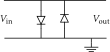
\includegraphics[scale=1.2]{report_img/diodes} 
		\caption{The double diode circuit is used to remove some of the amplitude of the signal before it is input to the mixer chip. This should allow a cleaner signal to be produced as the signal will be below the upper voltage limit of the chip.}
		\label{fig:diodes}
\end{figure} 

Another method to reduce the amplitude of the signal was attempted using a simple low pass filter. This time with a threshold frequency that is much higher than the wave which means that some of the frequencies that make up the square wave are removed. This will have the effect of reducing the overall amplitude of the wave, but at the expense of turning the square wave into a triangular wave. When implemented, this circuit had the desired effect of reducing the amplitude, but to such a degree that the signal is completely inaudible now. The amount of control over the properties of this circuit is limited and so this attempt is abandoned. 

\subsection{Quantitative Characteristics}
The nature of the variation of the produced signal with respect to the position of the user's hand is the product of several laws that govern separate components of the circuit. For example, the capacitance of the capacitor itself is inversely proportional to $d$ and the frequency of the oscillator chip is inversely proportional to $C$. This meant that the expect relation between the distance and the capacitance was
\begin{align}
	f &\propto \frac{1}{C} \propto \frac{1}{\frac{1}{d}} = d \nonumber \\
	\therefore f &\propto d 
\end{align}
This however was not seen when the frequency is measured with respect to the distance between the plates. When this was measured, shown in figure~\ref{fig:distance frequency}, the relation was found to be $f \propto \frac{1}{d}$.

\begin{figure}[ht]
	\centering
	\begin{minipage}[c]{0.3\textwidth}
		\begin{tabular}{r@{.}l|r@{.}l||r@{.}l|r@{.}l}
			\multicolumn{2}{c|}{\rotatebox{90}{Distance (cm)}} & \multicolumn{2}{c||}{\rotatebox{90}{Frequency (Hz)}} & \multicolumn{2}{c|}{\rotatebox{90}{Distance (cm)}} & \multicolumn{2}{c}{\rotatebox{90}{Frequency (Hz)}} \\ \hline \hline
			36&8	& 1&4 & 8&8	& 4&1 \\
			34&0	& 1&5 & 7&4	& 5&0 \\
			32&0	& 1&7 & 5&2	& 6&0 \\
			26&8	& 2&0 & 4&6	& 7&0 \\
			23&3	& 2&2 & 3&4	& 8&0 \\
			18&9	& 2&5 & 2&7	& 9&0 \\
			14&8	& 3&0 & 2&2	& 11&0 \\
			12&9	& 3&3 & 1&5	& 13&0 \\
			10&6	& 3&9 \\
		\end{tabular}
	\end{minipage}
	\begin{minipage}[c]{0.65\textwidth}
		\centering
		\centering
				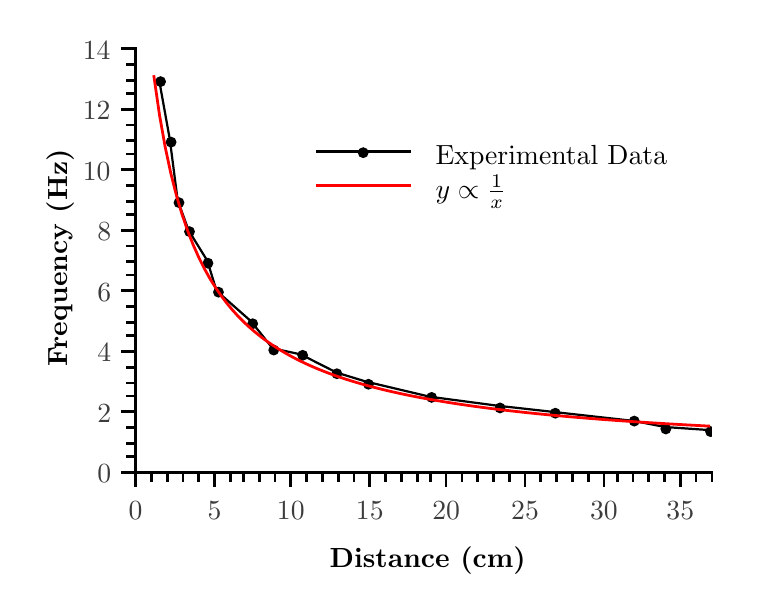
\begin{tikzpicture}{0pt}{0pt}{269pt}{209pt}
	\clip(0pt,209pt) -- (255.798pt,209pt) -- (255.798pt,10.2575pt) -- (0pt,10.2575pt) -- (0pt,209pt);
\begin{scope}
	\clip(38.9878pt,201.393pt) -- (247.239pt,201.393pt) -- (247.239pt,48.2943pt) -- (38.9878pt,48.2943pt) -- (38.9878pt,201.393pt);
	\color[rgb]{0,0,0}
	\draw[line width=0.8pt, line join=miter, line cap=rect](246.114pt,63.6042pt) -- (230.354pt,64.6977pt) -- (219.097pt,66.8848pt) -- (189.83pt,70.1655pt) -- (170.13pt,72.3526pt) -- (145.365pt,75.6333pt) -- (122.288pt,81.1011pt) -- (111.594pt,84.3818pt) -- (98.6491pt,90.9432pt) -- (88.5179pt,93.1303pt) -- (80.6381pt,102.972pt) -- (68.2556pt,113.908pt) -- (64.8785pt,124.843pt) -- (58.1244pt,135.779pt) -- (54.1845pt,146.715pt) -- (51.3703pt,168.586pt) -- (47.4304pt,190.457pt);
	\color[rgb]{0,0,0}
	\fill(246.764pt,63.0336pt) ellipse (1.42638pt and 1.42638pt);
	\draw[line width=1pt, line join=miter, line cap=rect](246.764pt,63.0336pt) ellipse (1.42638pt and 1.42638pt);
	\fill(230.598pt,63.9845pt) ellipse (1.42638pt and 1.42638pt);
	\draw[line width=1pt, line join=miter, line cap=rect](230.598pt,63.9845pt) ellipse (1.42638pt and 1.42638pt);
	\fill(219.187pt,66.8373pt) ellipse (1.42638pt and 1.42638pt);
	\draw[line width=1pt, line join=miter, line cap=rect](219.187pt,66.8373pt) ellipse (1.42638pt and 1.42638pt);
	\fill(190.66pt,69.6901pt) ellipse (1.42638pt and 1.42638pt);
	\draw[line width=1pt, line join=miter, line cap=rect](190.66pt,69.6901pt) ellipse (1.42638pt and 1.42638pt);
	\fill(170.69pt,71.5919pt) ellipse (1.42638pt and 1.42638pt);
	\draw[line width=1pt, line join=miter, line cap=rect](170.69pt,71.5919pt) ellipse (1.42638pt and 1.42638pt);
	\fill(145.966pt,75.3956pt) ellipse (1.42638pt and 1.42638pt);
	\draw[line width=1pt, line join=miter, line cap=rect](145.966pt,75.3956pt) ellipse (1.42638pt and 1.42638pt);
	\fill(123.144pt,80.1502pt) ellipse (1.42638pt and 1.42638pt);
	\draw[line width=1pt, line join=miter, line cap=rect](123.144pt,80.1502pt) ellipse (1.42638pt and 1.42638pt);
	\fill(111.733pt,83.9539pt) ellipse (1.42638pt and 1.42638pt);
	\draw[line width=1pt, line join=miter, line cap=rect](111.733pt,83.9539pt) ellipse (1.42638pt and 1.42638pt);
	\fill(99.3712pt,90.6103pt) ellipse (1.42638pt and 1.42638pt);
	\draw[line width=1pt, line join=miter, line cap=rect](99.3712pt,90.6103pt) ellipse (1.42638pt and 1.42638pt);
	\fill(88.9111pt,92.5122pt) ellipse (1.42638pt and 1.42638pt);
	\draw[line width=1pt, line join=miter, line cap=rect](88.9111pt,92.5122pt) ellipse (1.42638pt and 1.42638pt);
	\fill(81.3037pt,102.021pt) ellipse (1.42638pt and 1.42638pt);
	\draw[line width=1pt, line join=miter, line cap=rect](81.3037pt,102.021pt) ellipse (1.42638pt and 1.42638pt);
	\fill(68.9418pt,113.432pt) ellipse (1.42638pt and 1.42638pt);
	\draw[line width=1pt, line join=miter, line cap=rect](68.9418pt,113.432pt) ellipse (1.42638pt and 1.42638pt);
	\fill(65.1381pt,123.893pt) ellipse (1.42638pt and 1.42638pt);
	\draw[line width=1pt, line join=miter, line cap=rect](65.1381pt,123.893pt) ellipse (1.42638pt and 1.42638pt);
	\fill(58.4816pt,135.304pt) ellipse (1.42638pt and 1.42638pt);
	\draw[line width=1pt, line join=miter, line cap=rect](58.4816pt,135.304pt) ellipse (1.42638pt and 1.42638pt);
	\fill(54.678pt,145.764pt) ellipse (1.42638pt and 1.42638pt);
	\draw[line width=1pt, line join=miter, line cap=rect](54.678pt,145.764pt) ellipse (1.42638pt and 1.42638pt);
	\fill(51.8252pt,167.635pt) ellipse (1.42638pt and 1.42638pt);
	\draw[line width=1pt, line join=miter, line cap=rect](51.8252pt,167.635pt) ellipse (1.42638pt and 1.42638pt);
	\fill(48.0215pt,189.506pt) ellipse (1.42638pt and 1.42638pt);
	\draw[line width=1pt, line join=miter, line cap=rect](48.0215pt,189.506pt) ellipse (1.42638pt and 1.42638pt);
	\color[rgb]{1,0,0}
	\draw[line width=1pt, line join=bevel, line cap=rect](45.6293pt,191.317pt) -- (47.6544pt,177.335pt) -- (49.6795pt,165.934pt) -- (51.7046pt,156.458pt) -- (53.7297pt,148.459pt) -- (55.7548pt,141.616pt) -- (57.7799pt,135.695pt) -- (59.805pt,130.522pt) -- (61.8301pt,125.964pt) -- (63.8552pt,121.916pt) -- (65.8803pt,118.298pt) -- (67.9054pt,115.045pt) -- (69.9305pt,112.104pt) -- (71.9555pt,109.433pt) -- (73.9806pt,106.995pt) -- (76.0057pt,104.762pt) -- (78.0308pt,102.709pt) -- (80.0559pt,100.814pt) -- (82.081pt,99.0611pt) -- (84.1061pt,97.4339pt) -- (86.1312pt,95.9196pt) -- (88.1563pt,94.5067pt) -- (90.1814pt,93.1855pt) -- (92.2065pt,91.9472pt) -- (94.2316pt,90.7844pt) -- (96.2567pt,89.6903pt) -- (98.2818pt,88.659pt) -- (100.307pt,87.6853pt) -- (102.332pt,86.7644pt) -- (104.357pt,85.8922pt) -- (106.382pt,85.065pt) -- (108.407pt,84.2792pt) -- (110.432pt,83.5319pt) -- (112.457pt,82.8204pt) -- (114.483pt,82.1421pt) -- (116.508pt,81.4947pt) -- (118.533pt,80.8762pt) -- (120.558pt,80.2847pt) -- (122.583pt,79.7184pt) -- (124.608pt,79.1758pt) -- (126.633pt,78.6555pt) -- (128.658pt,78.156pt) -- (130.683pt,77.6762pt) -- (132.708pt,77.2148pt) -- (134.734pt,76.771pt) -- (136.759pt,76.3436pt) -- (138.784pt,75.9318pt) -- (140.809pt,75.5348pt) -- (142.834pt,75.1517pt) -- (144.859pt,74.7819pt) -- (146.884pt,74.4247pt) -- (148.909pt,74.0794pt) -- (150.934pt,73.7454pt) -- (152.959pt,73.4223pt) -- (154.984pt,73.1094pt) -- (157.01pt,72.8063pt) -- (159.035pt,72.5126pt) -- (161.06pt,72.2278pt) -- (163.085pt,71.9515pt) -- (165.11pt,71.6834pt) -- (167.135pt,71.4231pt) -- (169.16pt,71.1702pt) -- (171.185pt,70.9244pt) -- (173.21pt,70.6855pt) -- (175.235pt,70.4532pt) -- (177.261pt,70.2271pt) -- (179.286pt,70.0071pt) -- (181.311pt,69.7929pt) -- (183.336pt,69.5843pt) -- (185.361pt,69.381pt) -- (187.386pt,69.1829pt) -- (189.411pt,68.9898pt) -- (191.436pt,68.8014pt) -- (193.461pt,68.6176pt) -- (195.486pt,68.4383pt) -- (197.511pt,68.2632pt) -- (199.537pt,68.0923pt) -- (201.562pt,67.9254pt) -- (203.587pt,67.7623pt) -- (205.612pt,67.6029pt) -- (207.637pt,67.4471pt) -- (209.662pt,67.2948pt) -- (211.687pt,67.1458pt) -- (213.712pt,67.0001pt) -- (215.737pt,66.8575pt) -- (217.762pt,66.7179pt) -- (219.788pt,66.5813pt) -- (221.813pt,66.4475pt) -- (223.838pt,66.3166pt) -- (225.863pt,66.1882pt) -- (227.888pt,66.0625pt) -- (229.913pt,65.9393pt) -- (231.938pt,65.8186pt) -- (233.963pt,65.7002pt) -- (235.988pt,65.5841pt) -- (238.013pt,65.4702pt) -- (240.039pt,65.3586pt) -- (242.064pt,65.249pt) -- (244.089pt,65.1415pt) -- (246.114pt,65.0359pt);
\end{scope}
\begin{scope}
	\color[rgb]{0,0,0}
	\pgftext[center, base, at={\pgfpoint{14.2638pt}{125.794pt}},rotate=90]{\textbf{Frequency (Hz)}}
	\color[rgb]{0.235294,0.235294,0.235294}
	\pgftext[center, base, at={\pgfpoint{27.6881pt}{44.4907pt}}]{0}
	\pgftext[center, base, at={\pgfpoint{27.6881pt}{66.3618pt}}]{2}
	\pgftext[center, base, at={\pgfpoint{27.6881pt}{88.233pt}}]{4}
	\pgftext[center, base, at={\pgfpoint{27.6881pt}{110.104pt}}]{6}
	\pgftext[center, base, at={\pgfpoint{27.6881pt}{131.975pt}}]{8}
	\pgftext[center, base, at={\pgfpoint{24.9468pt}{153.847pt}}]{10}
	\pgftext[center, base, at={\pgfpoint{24.9468pt}{175.718pt}}]{12}
	\pgftext[center, base, at={\pgfpoint{24.9468pt}{197.589pt}}]{14}
	\color[rgb]{0,0,0}
	\draw[line width=1pt, line join=bevel, line cap=rect](38.9878pt,53.9999pt) -- (36.135pt,53.9999pt);
	\draw[line width=1pt, line join=bevel, line cap=rect](38.9878pt,64.46pt) -- (36.135pt,64.46pt);
	\draw[line width=1pt, line join=bevel, line cap=rect](38.9878pt,75.8711pt) -- (36.135pt,75.8711pt);
	\draw[line width=1pt, line join=bevel, line cap=rect](38.9878pt,86.3312pt) -- (36.135pt,86.3312pt);
	\draw[line width=1pt, line join=bevel, line cap=rect](38.9878pt,97.7422pt) -- (36.135pt,97.7422pt);
	\draw[line width=1pt, line join=bevel, line cap=rect](38.9878pt,108.202pt) -- (36.135pt,108.202pt);
	\draw[line width=1pt, line join=bevel, line cap=rect](38.9878pt,119.613pt) -- (36.135pt,119.613pt);
	\draw[line width=1pt, line join=bevel, line cap=rect](38.9878pt,130.074pt) -- (36.135pt,130.074pt);
	\draw[line width=1pt, line join=bevel, line cap=rect](38.9878pt,141.485pt) -- (36.135pt,141.485pt);
	\draw[line width=1pt, line join=bevel, line cap=rect](38.9878pt,151.945pt) -- (36.135pt,151.945pt);
	\draw[line width=1pt, line join=bevel, line cap=rect](38.9878pt,163.356pt) -- (36.135pt,163.356pt);
	\draw[line width=1pt, line join=bevel, line cap=rect](38.9878pt,173.816pt) -- (36.135pt,173.816pt);
	\draw[line width=1pt, line join=bevel, line cap=rect](38.9878pt,185.227pt) -- (36.135pt,185.227pt);
	\draw[line width=1pt, line join=bevel, line cap=rect](38.9878pt,195.687pt) -- (36.135pt,195.687pt);
	\draw[line width=1pt, line join=bevel, line cap=rect](38.9878pt,58.7545pt) -- (36.135pt,58.7545pt);
	\draw[line width=1pt, line join=bevel, line cap=rect](38.9878pt,80.6257pt) -- (36.135pt,80.6257pt);
	\draw[line width=1pt, line join=bevel, line cap=rect](38.9878pt,102.497pt) -- (36.135pt,102.497pt);
	\draw[line width=1pt, line join=bevel, line cap=rect](38.9878pt,124.368pt) -- (36.135pt,124.368pt);
	\draw[line width=1pt, line join=bevel, line cap=rect](38.9878pt,146.239pt) -- (36.135pt,146.239pt);
	\draw[line width=1pt, line join=bevel, line cap=rect](38.9878pt,168.11pt) -- (36.135pt,168.11pt);
	\draw[line width=1pt, line join=bevel, line cap=rect](38.9878pt,189.982pt) -- (36.135pt,189.982pt);
	\draw[line width=1pt, line join=bevel, line cap=rect](38.9878pt,48.2943pt) -- (34.2332pt,48.2943pt);
	\draw[line width=1pt, line join=bevel, line cap=rect](38.9878pt,70.1655pt) -- (34.2332pt,70.1655pt);
	\draw[line width=1pt, line join=bevel, line cap=rect](38.9878pt,92.0367pt) -- (34.2332pt,92.0367pt);
	\draw[line width=1pt, line join=bevel, line cap=rect](38.9878pt,113.908pt) -- (34.2332pt,113.908pt);
	\draw[line width=1pt, line join=bevel, line cap=rect](38.9878pt,135.779pt) -- (34.2332pt,135.779pt);
	\draw[line width=1pt, line join=bevel, line cap=rect](38.9878pt,157.65pt) -- (34.2332pt,157.65pt);
	\draw[line width=1pt, line join=bevel, line cap=rect](38.9878pt,179.521pt) -- (34.2332pt,179.521pt);
	\draw[line width=1pt, line join=bevel, line cap=rect](38.9878pt,201.393pt) -- (34.2332pt,201.393pt);
	\draw[line width=1pt, line join=bevel, line cap=rect](38.9878pt,201.393pt) -- (38.9878pt,48.2943pt);
	\pgftext[center, base, at={\pgfpoint{144.533pt}{14.0612pt}}]{\textbf{Distance (cm)}}
	\color[rgb]{0.235294,0.235294,0.235294}
	\pgftext[center, base, at={\pgfpoint{38.9803pt}{31.1778pt}}]{0}
	\pgftext[center, base, at={\pgfpoint{67.508pt}{31.1778pt}}]{5}
	\pgftext[center, base, at={\pgfpoint{95.0921pt}{31.1778pt}}]{10}
	\pgftext[center, base, at={\pgfpoint{123.62pt}{31.1778pt}}]{15}
	\pgftext[center, base, at={\pgfpoint{151.196pt}{31.1778pt}}]{20}
	\pgftext[center, base, at={\pgfpoint{179.724pt}{31.1778pt}}]{25}
	\pgftext[center, base, at={\pgfpoint{208.252pt}{31.1778pt}}]{30}
	\pgftext[center, base, at={\pgfpoint{235.828pt}{31.1778pt}}]{35}
	\color[rgb]{0,0,0}
	\draw[line width=1pt, line join=bevel, line cap=rect](44.6933pt,48.2943pt) -- (44.6933pt,45.4416pt);
	\draw[line width=1pt, line join=bevel, line cap=rect](50.3988pt,48.2943pt) -- (50.3988pt,45.4416pt);
	\draw[line width=1pt, line join=bevel, line cap=rect](56.1043pt,48.2943pt) -- (56.1043pt,45.4416pt);
	\draw[line width=1pt, line join=bevel, line cap=rect](61.8099pt,48.2943pt) -- (61.8099pt,45.4416pt);
	\draw[line width=1pt, line join=bevel, line cap=rect](73.2209pt,48.2943pt) -- (73.2209pt,45.4416pt);
	\draw[line width=1pt, line join=bevel, line cap=rect](77.9755pt,48.2943pt) -- (77.9755pt,45.4416pt);
	\draw[line width=1pt, line join=bevel, line cap=rect](83.6811pt,48.2943pt) -- (83.6811pt,45.4416pt);
	\draw[line width=1pt, line join=bevel, line cap=rect](89.3866pt,48.2943pt) -- (89.3866pt,45.4416pt);
	\draw[line width=1pt, line join=bevel, line cap=rect](100.798pt,48.2943pt) -- (100.798pt,45.4416pt);
	\draw[line width=1pt, line join=bevel, line cap=rect](106.503pt,48.2943pt) -- (106.503pt,45.4416pt);
	\draw[line width=1pt, line join=bevel, line cap=rect](112.209pt,48.2943pt) -- (112.209pt,45.4416pt);
	\draw[line width=1pt, line join=bevel, line cap=rect](117.914pt,48.2943pt) -- (117.914pt,45.4416pt);
	\draw[line width=1pt, line join=bevel, line cap=rect](129.325pt,48.2943pt) -- (129.325pt,45.4416pt);
	\draw[line width=1pt, line join=bevel, line cap=rect](135.031pt,48.2943pt) -- (135.031pt,45.4416pt);
	\draw[line width=1pt, line join=bevel, line cap=rect](140.736pt,48.2943pt) -- (140.736pt,45.4416pt);
	\draw[line width=1pt, line join=bevel, line cap=rect](145.491pt,48.2943pt) -- (145.491pt,45.4416pt);
	\draw[line width=1pt, line join=bevel, line cap=rect](156.902pt,48.2943pt) -- (156.902pt,45.4416pt);
	\draw[line width=1pt, line join=bevel, line cap=rect](162.607pt,48.2943pt) -- (162.607pt,45.4416pt);
	\draw[line width=1pt, line join=bevel, line cap=rect](168.313pt,48.2943pt) -- (168.313pt,45.4416pt);
	\draw[line width=1pt, line join=bevel, line cap=rect](174.019pt,48.2943pt) -- (174.019pt,45.4416pt);
	\draw[line width=1pt, line join=bevel, line cap=rect](185.43pt,48.2943pt) -- (185.43pt,45.4416pt);
	\draw[line width=1pt, line join=bevel, line cap=rect](191.135pt,48.2943pt) -- (191.135pt,45.4416pt);
	\draw[line width=1pt, line join=bevel, line cap=rect](196.841pt,48.2943pt) -- (196.841pt,45.4416pt);
	\draw[line width=1pt, line join=bevel, line cap=rect](202.546pt,48.2943pt) -- (202.546pt,45.4416pt);
	\draw[line width=1pt, line join=bevel, line cap=rect](213.006pt,48.2943pt) -- (213.006pt,45.4416pt);
	\draw[line width=1pt, line join=bevel, line cap=rect](218.712pt,48.2943pt) -- (218.712pt,45.4416pt);
	\draw[line width=1pt, line join=bevel, line cap=rect](224.417pt,48.2943pt) -- (224.417pt,45.4416pt);
	\draw[line width=1pt, line join=bevel, line cap=rect](230.123pt,48.2943pt) -- (230.123pt,45.4416pt);
	\draw[line width=1pt, line join=bevel, line cap=rect](241.534pt,48.2943pt) -- (241.534pt,45.4416pt);
	\draw[line width=1pt, line join=bevel, line cap=rect](247.239pt,48.2943pt) -- (247.239pt,45.4416pt);
	\draw[line width=1pt, line join=bevel, line cap=rect](38.9878pt,48.2943pt) -- (38.9878pt,43.5397pt);
	\draw[line width=1pt, line join=bevel, line cap=rect](67.5154pt,48.2943pt) -- (67.5154pt,43.5397pt);
	\draw[line width=1pt, line join=bevel, line cap=rect](95.0921pt,48.2943pt) -- (95.0921pt,43.5397pt);
	\draw[line width=1pt, line join=bevel, line cap=rect](123.62pt,48.2943pt) -- (123.62pt,43.5397pt);
	\draw[line width=1pt, line join=bevel, line cap=rect](151.196pt,48.2943pt) -- (151.196pt,43.5397pt);
	\draw[line width=1pt, line join=bevel, line cap=rect](179.724pt,48.2943pt) -- (179.724pt,43.5397pt);
	\draw[line width=1pt, line join=bevel, line cap=rect](208.252pt,48.2943pt) -- (208.252pt,43.5397pt);
	\draw[line width=1pt, line join=bevel, line cap=rect](235.828pt,48.2943pt) -- (235.828pt,43.5397pt);
	\draw[line width=1pt, line join=bevel, line cap=rect](38.9878pt,48.2943pt) -- (247.239pt,48.2943pt);
	\draw[line width=1pt, line join=miter, line cap=rect](104.601pt,164.307pt) -- (137.884pt,164.307pt);
	\fill(121.242pt,163.831pt) ellipse (1.42638pt and 1.42638pt);
	\draw[line width=1pt, line join=miter, line cap=rect](121.242pt,163.831pt) ellipse (1.42638pt and 1.42638pt);
	\pgftext[left, base, at={\pgfpoint{147.393pt}{159.552pt}}]{Experimental Data}
	\color[rgb]{1,0,0}
	\draw[line width=1pt, line join=bevel, line cap=rect](104.601pt,151.945pt) -- (137.884pt,151.945pt);
	\color[rgb]{0,0,0}
	\pgftext[left, base, at={\pgfpoint{147.393pt}{147.19pt}}]{$y \propto \frac{1}{x}$}
\end{scope}
\end{tikzpicture}
 
			\vspace{-10pt}
	\end{minipage}
	\caption{The distance from the plate capacitor against the frequency that this position produces is recorded.}
	\label{fig:distance frequency}
\end{figure}

Also, the action of the mixer chip was verified by measuring the output frequency produced when using a single VCO at a fixed frequency of 1.5\,MHz and the variable TG315 signal generator. This is shown in figure~\ref{fig:frequency generator}. The linear direct relationship can be clearly seen here. This graph is of the form $y=|x-c|$ where $c$ is a constant, since the two regions have the same slope. This confirms that the action of the mixer is as expected.  

\begin{figure}
	\begin{center}
		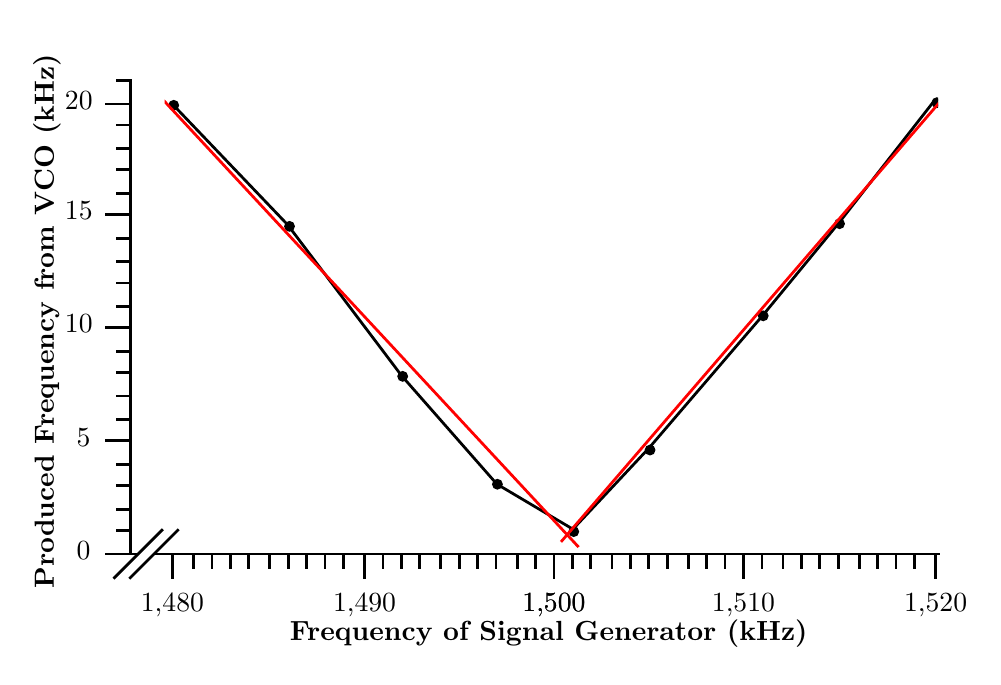
\begin{tikzpicture}{0pt}{0pt}{359pt}{239pt}
	\clip(0pt,239pt) -- (341.381pt,239pt) -- (341.381pt,11.7299pt) -- (0pt,11.7299pt) -- (0pt,239pt);
\begin{scope}
	\clip(49.4479pt,219.982pt) -- (329.019pt,219.982pt) -- (329.019pt,48.8158pt) -- (49.4479pt,48.8158pt) -- (49.4479pt,219.982pt);
	\color[rgb]{0,0,0}
	\draw[line width=1pt, line join=miter, line cap=rect](52.6521pt,211.016pt) -- (93.9009pt,167.817pt) -- (135.15pt,113.207pt) -- (169.524pt,74.0831pt) -- (197.023pt,57.7816pt) -- (224.522pt,87.1243pt) -- (265.771pt,135.214pt) -- (293.27pt,168.632pt) -- (327.644pt,212.646pt);
	\color[rgb]{0,0,0}
	\fill(52.7761pt,210.948pt) ellipse (1.42638pt and 1.42638pt);
	\draw[line width=1pt, line join=miter, line cap=rect](52.7761pt,210.948pt) ellipse (1.42638pt and 1.42638pt);
	\fill(94.6166pt,167.205pt) ellipse (1.42638pt and 1.42638pt);
	\draw[line width=1pt, line join=miter, line cap=rect](94.6166pt,167.205pt) ellipse (1.42638pt and 1.42638pt);
	\fill(135.506pt,113.003pt) ellipse (1.42638pt and 1.42638pt);
	\draw[line width=1pt, line join=miter, line cap=rect](135.506pt,113.003pt) ellipse (1.42638pt and 1.42638pt);
	\fill(169.739pt,74.0152pt) ellipse (1.42638pt and 1.42638pt);
	\draw[line width=1pt, line join=miter, line cap=rect](169.739pt,74.0152pt) ellipse (1.42638pt and 1.42638pt);
	\fill(197.316pt,56.8986pt) ellipse (1.42638pt and 1.42638pt);
	\draw[line width=1pt, line join=miter, line cap=rect](197.316pt,56.8986pt) ellipse (1.42638pt and 1.42638pt);
	\fill(224.893pt,86.3772pt) ellipse (1.42638pt and 1.42638pt);
	\draw[line width=1pt, line join=miter, line cap=rect](224.893pt,86.3772pt) ellipse (1.42638pt and 1.42638pt);
	\fill(265.782pt,134.874pt) ellipse (1.42638pt and 1.42638pt);
	\draw[line width=1pt, line join=miter, line cap=rect](265.782pt,134.874pt) ellipse (1.42638pt and 1.42638pt);
	\fill(293.359pt,168.156pt) ellipse (1.42638pt and 1.42638pt);
	\draw[line width=1pt, line join=miter, line cap=rect](293.359pt,168.156pt) ellipse (1.42638pt and 1.42638pt);
	\fill(328.543pt,211.899pt) ellipse (1.42638pt and 1.42638pt);
	\draw[line width=1pt, line join=miter, line cap=rect](328.543pt,211.899pt) ellipse (1.42638pt and 1.42638pt);
	\color[rgb]{1,0,0}
	\draw[line width=1pt, line join=miter, line cap=rect](334.724pt,218.08pt) -- (193.037pt,53.5704pt);
	\draw[line width=1pt, line join=miter, line cap=rect](49.4479pt,212.374pt) -- (198.742pt,51.6686pt);
\end{scope}
\begin{scope}
	\color[rgb]{0,0,0}
	\pgftext[center, base, at={\pgfpoint{188.275pt}{227.589pt}}]{\textbf{ }}
	\color[rgb]{0,0,0}
	\pgftext[center, base, at={\pgfpoint{9.50921pt}{132.972pt}},rotate=90]{\textbf{Produced Frequency from VCO (kHz)}}
	\pgftext[center, base, at={\pgfpoint{20.1774pt}{46.9139pt}}]{0}
	\pgftext[center, base, at={\pgfpoint{20.1774pt}{87.8036pt}}]{5}
	\pgftext[center, base, at={\pgfpoint{18.4835pt}{128.693pt}}]{10}
	\pgftext[center, base, at={\pgfpoint{18.4835pt}{169.583pt}}]{15}
	\pgftext[center, base, at={\pgfpoint{18.4835pt}{209.521pt}}]{20}
	\draw[line width=1pt, line join=bevel, line cap=rect](37.0859pt,57.3741pt) -- (32.3313pt,57.3741pt);
	\draw[line width=1pt, line join=bevel, line cap=rect](37.0859pt,64.9814pt) -- (32.3313pt,64.9814pt);
	\draw[line width=1pt, line join=bevel, line cap=rect](37.0859pt,73.5397pt) -- (32.3313pt,73.5397pt);
	\draw[line width=1pt, line join=bevel, line cap=rect](37.0859pt,81.1471pt) -- (32.3313pt,81.1471pt);
	\draw[line width=1pt, line join=bevel, line cap=rect](37.0859pt,97.3128pt) -- (32.3313pt,97.3128pt);
	\draw[line width=1pt, line join=bevel, line cap=rect](37.0859pt,105.871pt) -- (32.3313pt,105.871pt);
	\draw[line width=1pt, line join=bevel, line cap=rect](37.0859pt,114.429pt) -- (32.3313pt,114.429pt);
	\draw[line width=1pt, line join=bevel, line cap=rect](37.0859pt,122.037pt) -- (32.3313pt,122.037pt);
	\draw[line width=1pt, line join=bevel, line cap=rect](37.0859pt,138.202pt) -- (32.3313pt,138.202pt);
	\draw[line width=1pt, line join=bevel, line cap=rect](37.0859pt,146.761pt) -- (32.3313pt,146.761pt);
	\draw[line width=1pt, line join=bevel, line cap=rect](37.0859pt,154.368pt) -- (32.3313pt,154.368pt);
	\draw[line width=1pt, line join=bevel, line cap=rect](37.0859pt,162.926pt) -- (32.3313pt,162.926pt);
	\draw[line width=1pt, line join=bevel, line cap=rect](37.0859pt,179.092pt) -- (32.3313pt,179.092pt);
	\draw[line width=1pt, line join=bevel, line cap=rect](37.0859pt,187.65pt) -- (32.3313pt,187.65pt);
	\draw[line width=1pt, line join=bevel, line cap=rect](37.0859pt,195.258pt) -- (32.3313pt,195.258pt);
	\draw[line width=1pt, line join=bevel, line cap=rect](37.0859pt,203.816pt) -- (32.3313pt,203.816pt);
	\draw[line width=1pt, line join=bevel, line cap=rect](37.0859pt,219.982pt) -- (32.3313pt,219.982pt);
	\draw[line width=1pt, line join=bevel, line cap=rect](37.0859pt,48.8158pt) -- (28.5276pt,48.8158pt);
	\draw[line width=1pt, line join=bevel, line cap=rect](37.0859pt,89.7054pt) -- (28.5276pt,89.7054pt);
	\draw[line width=1pt, line join=bevel, line cap=rect](37.0859pt,130.595pt) -- (28.5276pt,130.595pt);
	\draw[line width=1pt, line join=bevel, line cap=rect](37.0859pt,171.485pt) -- (28.5276pt,171.485pt);
	\draw[line width=1pt, line join=bevel, line cap=rect](37.0859pt,211.423pt) -- (28.5276pt,211.423pt);
	\draw[line width=1pt, line join=bevel, line cap=rect](37.0859pt,219.982pt) -- (37.0859pt,48.8158pt);
	\pgftext[center, base, at={\pgfpoint{188.275pt}{17.4354pt}}]{\textbf{Frequency of Signal Generator (kHz)}}
	\draw[line width=1pt, line join=bevel, line cap=rect](48.497pt,57.3741pt) -- (31.3804pt,40.2575pt);
	\draw[line width=1pt, line join=bevel, line cap=rect](54.2025pt,57.3741pt) -- (37.0859pt,40.2575pt);
	\pgftext[center, base, at={\pgfpoint{190.184pt}{27.8955pt}}]{1,500}
	\pgftext[center, base, at={\pgfpoint{52.3007pt}{27.8955pt}}]{1,480}
	\pgftext[center, base, at={\pgfpoint{121.718pt}{27.8955pt}}]{1,490}
	\pgftext[center, base, at={\pgfpoint{190.184pt}{27.8955pt}}]{1,500}
	\pgftext[center, base, at={\pgfpoint{258.651pt}{27.8955pt}}]{1,510}
	\pgftext[center, base, at={\pgfpoint{328.068pt}{27.8955pt}}]{1,520}
	\draw[line width=1pt, line join=bevel, line cap=rect](59.908pt,48.8158pt) -- (59.908pt,44.0612pt);
	\draw[line width=1pt, line join=bevel, line cap=rect](66.5645pt,48.8158pt) -- (66.5645pt,44.0612pt);
	\draw[line width=1pt, line join=bevel, line cap=rect](73.2209pt,48.8158pt) -- (73.2209pt,44.0612pt);
	\draw[line width=1pt, line join=bevel, line cap=rect](79.8774pt,48.8158pt) -- (79.8774pt,44.0612pt);
	\draw[line width=1pt, line join=bevel, line cap=rect](94.1412pt,48.8158pt) -- (94.1412pt,44.0612pt);
	\draw[line width=1pt, line join=bevel, line cap=rect](100.798pt,48.8158pt) -- (100.798pt,44.0612pt);
	\draw[line width=1pt, line join=bevel, line cap=rect](107.454pt,48.8158pt) -- (107.454pt,44.0612pt);
	\draw[line width=1pt, line join=bevel, line cap=rect](114.111pt,48.8158pt) -- (114.111pt,44.0612pt);
	\draw[line width=1pt, line join=bevel, line cap=rect](128.374pt,48.8158pt) -- (128.374pt,44.0612pt);
	\draw[line width=1pt, line join=bevel, line cap=rect](135.031pt,48.8158pt) -- (135.031pt,44.0612pt);
	\draw[line width=1pt, line join=bevel, line cap=rect](141.687pt,48.8158pt) -- (141.687pt,44.0612pt);
	\draw[line width=1pt, line join=bevel, line cap=rect](149.295pt,48.8158pt) -- (149.295pt,44.0612pt);
	\draw[line width=1pt, line join=bevel, line cap=rect](162.607pt,48.8158pt) -- (162.607pt,44.0612pt);
	\draw[line width=1pt, line join=bevel, line cap=rect](169.264pt,48.8158pt) -- (169.264pt,44.0612pt);
	\draw[line width=1pt, line join=bevel, line cap=rect](176.871pt,48.8158pt) -- (176.871pt,44.0612pt);
	\draw[line width=1pt, line join=bevel, line cap=rect](183.528pt,48.8158pt) -- (183.528pt,44.0612pt);
	\draw[line width=1pt, line join=bevel, line cap=rect](196.841pt,48.8158pt) -- (196.841pt,44.0612pt);
	\draw[line width=1pt, line join=bevel, line cap=rect](203.497pt,48.8158pt) -- (203.497pt,44.0612pt);
	\draw[line width=1pt, line join=bevel, line cap=rect](211.104pt,48.8158pt) -- (211.104pt,44.0612pt);
	\draw[line width=1pt, line join=bevel, line cap=rect](217.761pt,48.8158pt) -- (217.761pt,44.0612pt);
	\draw[line width=1pt, line join=bevel, line cap=rect](231.074pt,48.8158pt) -- (231.074pt,44.0612pt);
	\draw[line width=1pt, line join=bevel, line cap=rect](238.681pt,48.8158pt) -- (238.681pt,44.0612pt);
	\draw[line width=1pt, line join=bevel, line cap=rect](245.338pt,48.8158pt) -- (245.338pt,44.0612pt);
	\draw[line width=1pt, line join=bevel, line cap=rect](251.994pt,48.8158pt) -- (251.994pt,44.0612pt);
	\draw[line width=1pt, line join=bevel, line cap=rect](265.307pt,48.8158pt) -- (265.307pt,44.0612pt);
	\draw[line width=1pt, line join=bevel, line cap=rect](272.914pt,48.8158pt) -- (272.914pt,44.0612pt);
	\draw[line width=1pt, line join=bevel, line cap=rect](279.571pt,48.8158pt) -- (279.571pt,44.0612pt);
	\draw[line width=1pt, line join=bevel, line cap=rect](286.227pt,48.8158pt) -- (286.227pt,44.0612pt);
	\draw[line width=1pt, line join=bevel, line cap=rect](300.491pt,48.8158pt) -- (300.491pt,44.0612pt);
	\draw[line width=1pt, line join=bevel, line cap=rect](307.147pt,48.8158pt) -- (307.147pt,44.0612pt);
	\draw[line width=1pt, line join=bevel, line cap=rect](313.804pt,48.8158pt) -- (313.804pt,44.0612pt);
	\draw[line width=1pt, line join=bevel, line cap=rect](320.46pt,48.8158pt) -- (320.46pt,44.0612pt);
	\draw[line width=1pt, line join=bevel, line cap=rect](87.4847pt,48.8158pt) -- (87.4847pt,44.0612pt);
	\draw[line width=1pt, line join=bevel, line cap=rect](155.951pt,48.8158pt) -- (155.951pt,44.0612pt);
	\draw[line width=1pt, line join=bevel, line cap=rect](224.417pt,48.8158pt) -- (224.417pt,44.0612pt);
	\draw[line width=1pt, line join=bevel, line cap=rect](292.884pt,48.8158pt) -- (292.884pt,44.0612pt);
	\draw[line width=1pt, line join=bevel, line cap=rect](190.184pt,48.8158pt) -- (190.184pt,40.2575pt);
	\draw[line width=1pt, line join=bevel, line cap=rect](52.3007pt,48.8158pt) -- (52.3007pt,40.2575pt);
	\draw[line width=1pt, line join=bevel, line cap=rect](121.718pt,48.8158pt) -- (121.718pt,40.2575pt);
	\draw[line width=1pt, line join=bevel, line cap=rect](190.184pt,48.8158pt) -- (190.184pt,40.2575pt);
	\draw[line width=1pt, line join=bevel, line cap=rect](258.651pt,48.8158pt) -- (258.651pt,40.2575pt);
	\draw[line width=1pt, line join=bevel, line cap=rect](328.068pt,48.8158pt) -- (328.068pt,40.2575pt);
	\draw[line width=1pt, line join=bevel, line cap=rect](37.0859pt,48.8158pt) -- (38.9878pt,48.8158pt);
	\draw[line width=1pt, line join=bevel, line cap=rect](46.5951pt,48.8158pt) -- (329.019pt,48.8158pt);
\end{scope}
\end{tikzpicture}

		\caption{As the generator input frequency to the mixer is increased, the difference between the generator and the reference VCO decreases, and so does the output frequency produced, until the generator is greater than the reference and so the difference, and so the output frequency, increases.}
		\label{fig:frequency generator}
	\end{center}
\end{figure}

Finally the relationship between the frequency of the input to the low pass circuit and the peak to peak voltage of the output of low pass circuit was measured. This allowed the characteristics of the signal with respect to the voltage to be observed. As can be seen in figure~\ref{fig:bode}, this is essentially a Bode plot with a cut off frequency of around 23.5\,kHz, just above human hearing range. This confirmed what was expected. As the frequency increases, the voltage is almost constant, up until the cut off frequency where the voltage is attenuated swiftly. This is due to the effect of the low pass filter removing the high frequency signals as desired.

\begin{figure}
	\begin{center}
		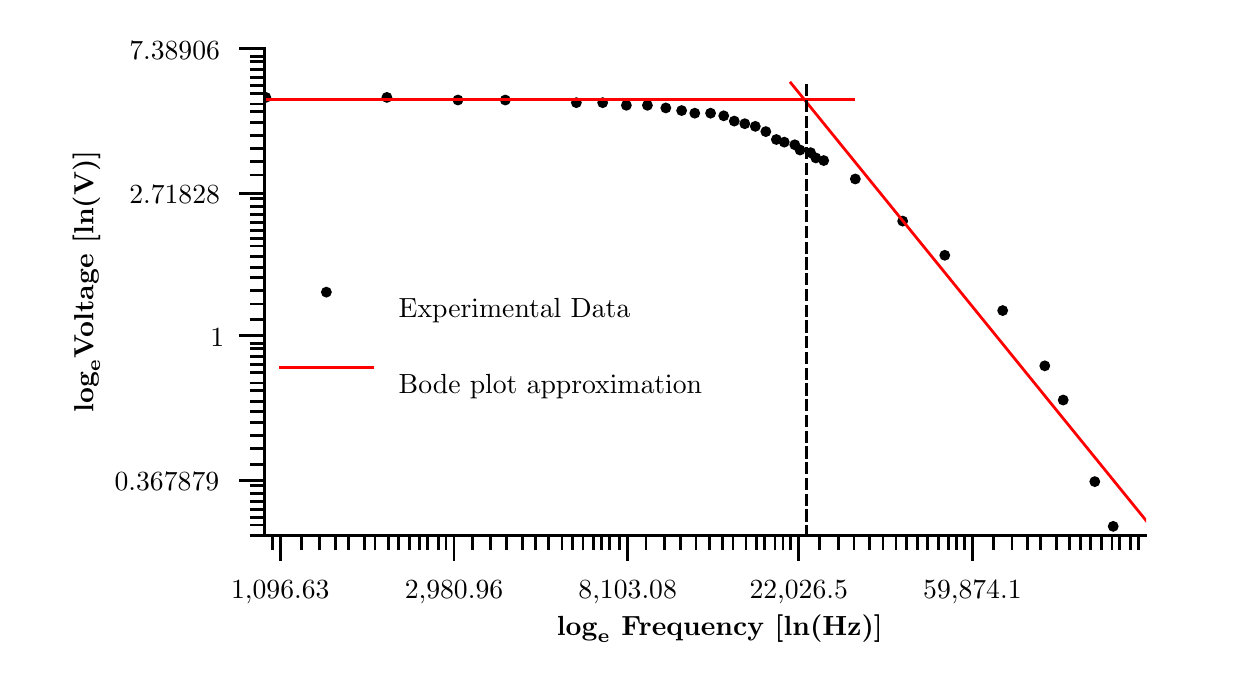
\begin{tikzpicture}{0pt}{0pt}{449pt}{239pt}
	\clip(0pt,239pt) -- (426.964pt,239pt) -- (426.964pt,11.7299pt) -- (0pt,11.7299pt) -- (0pt,239pt);
\begin{scope}
	\clip(85.5829pt,231.393pt) -- (404.141pt,231.393pt) -- (404.141pt,55.4722pt) -- (85.5829pt,55.4722pt) -- (85.5829pt,231.393pt);
	\color[rgb]{0,0,0}
	\fill(86.0584pt,213.801pt) ellipse (1.42638pt and 1.42638pt);
	\draw[line width=1pt, line join=miter, line cap=rect](86.0584pt,213.801pt) ellipse (1.42638pt and 1.42638pt);
	\color[rgb]{0,0,0}
	\fill(129.801pt,213.801pt) ellipse (1.42638pt and 1.42638pt);
	\draw[line width=1pt, line join=miter, line cap=rect](129.801pt,213.801pt) ellipse (1.42638pt and 1.42638pt);
	\fill(155.476pt,212.85pt) ellipse (1.42638pt and 1.42638pt);
	\draw[line width=1pt, line join=miter, line cap=rect](155.476pt,212.85pt) ellipse (1.42638pt and 1.42638pt);
	\fill(172.592pt,212.85pt) ellipse (1.42638pt and 1.42638pt);
	\draw[line width=1pt, line join=miter, line cap=rect](172.592pt,212.85pt) ellipse (1.42638pt and 1.42638pt);
	\fill(198.267pt,211.899pt) ellipse (1.42638pt and 1.42638pt);
	\draw[line width=1pt, line join=miter, line cap=rect](198.267pt,211.899pt) ellipse (1.42638pt and 1.42638pt);
	\fill(207.776pt,211.899pt) ellipse (1.42638pt and 1.42638pt);
	\draw[line width=1pt, line join=miter, line cap=rect](207.776pt,211.899pt) ellipse (1.42638pt and 1.42638pt);
	\fill(216.335pt,210.948pt) ellipse (1.42638pt and 1.42638pt);
	\draw[line width=1pt, line join=miter, line cap=rect](216.335pt,210.948pt) ellipse (1.42638pt and 1.42638pt);
	\fill(223.942pt,210.948pt) ellipse (1.42638pt and 1.42638pt);
	\draw[line width=1pt, line join=miter, line cap=rect](223.942pt,210.948pt) ellipse (1.42638pt and 1.42638pt);
	\fill(230.598pt,209.997pt) ellipse (1.42638pt and 1.42638pt);
	\draw[line width=1pt, line join=miter, line cap=rect](230.598pt,209.997pt) ellipse (1.42638pt and 1.42638pt);
	\fill(236.304pt,209.046pt) ellipse (1.42638pt and 1.42638pt);
	\draw[line width=1pt, line join=miter, line cap=rect](236.304pt,209.046pt) ellipse (1.42638pt and 1.42638pt);
	\fill(241.058pt,208.095pt) ellipse (1.42638pt and 1.42638pt);
	\draw[line width=1pt, line join=miter, line cap=rect](241.058pt,208.095pt) ellipse (1.42638pt and 1.42638pt);
	\fill(246.764pt,208.095pt) ellipse (1.42638pt and 1.42638pt);
	\draw[line width=1pt, line join=miter, line cap=rect](246.764pt,208.095pt) ellipse (1.42638pt and 1.42638pt);
	\fill(251.519pt,207.144pt) ellipse (1.42638pt and 1.42638pt);
	\draw[line width=1pt, line join=miter, line cap=rect](251.519pt,207.144pt) ellipse (1.42638pt and 1.42638pt);
	\fill(255.322pt,205.242pt) ellipse (1.42638pt and 1.42638pt);
	\draw[line width=1pt, line join=miter, line cap=rect](255.322pt,205.242pt) ellipse (1.42638pt and 1.42638pt);
	\fill(259.126pt,204.291pt) ellipse (1.42638pt and 1.42638pt);
	\draw[line width=1pt, line join=miter, line cap=rect](259.126pt,204.291pt) ellipse (1.42638pt and 1.42638pt);
	\fill(262.93pt,203.34pt) ellipse (1.42638pt and 1.42638pt);
	\draw[line width=1pt, line join=miter, line cap=rect](262.93pt,203.34pt) ellipse (1.42638pt and 1.42638pt);
	\fill(266.733pt,201.439pt) ellipse (1.42638pt and 1.42638pt);
	\draw[line width=1pt, line join=miter, line cap=rect](266.733pt,201.439pt) ellipse (1.42638pt and 1.42638pt);
	\fill(270.537pt,198.586pt) ellipse (1.42638pt and 1.42638pt);
	\draw[line width=1pt, line join=miter, line cap=rect](270.537pt,198.586pt) ellipse (1.42638pt and 1.42638pt);
	\fill(273.39pt,197.635pt) ellipse (1.42638pt and 1.42638pt);
	\draw[line width=1pt, line join=miter, line cap=rect](273.39pt,197.635pt) ellipse (1.42638pt and 1.42638pt);
	\fill(277.193pt,196.684pt) ellipse (1.42638pt and 1.42638pt);
	\draw[line width=1pt, line join=miter, line cap=rect](277.193pt,196.684pt) ellipse (1.42638pt and 1.42638pt);
	\fill(279.095pt,194.782pt) ellipse (1.42638pt and 1.42638pt);
	\draw[line width=1pt, line join=miter, line cap=rect](279.095pt,194.782pt) ellipse (1.42638pt and 1.42638pt);
	\fill(282.899pt,193.831pt) ellipse (1.42638pt and 1.42638pt);
	\draw[line width=1pt, line join=miter, line cap=rect](282.899pt,193.831pt) ellipse (1.42638pt and 1.42638pt);
	\fill(284.801pt,191.929pt) ellipse (1.42638pt and 1.42638pt);
	\draw[line width=1pt, line join=miter, line cap=rect](284.801pt,191.929pt) ellipse (1.42638pt and 1.42638pt);
	\fill(287.654pt,190.978pt) ellipse (1.42638pt and 1.42638pt);
	\draw[line width=1pt, line join=miter, line cap=rect](287.654pt,190.978pt) ellipse (1.42638pt and 1.42638pt);
	\fill(299.065pt,184.322pt) ellipse (1.42638pt and 1.42638pt);
	\draw[line width=1pt, line join=miter, line cap=rect](299.065pt,184.322pt) ellipse (1.42638pt and 1.42638pt);
	\fill(316.181pt,169.107pt) ellipse (1.42638pt and 1.42638pt);
	\draw[line width=1pt, line join=miter, line cap=rect](316.181pt,169.107pt) ellipse (1.42638pt and 1.42638pt);
	\fill(331.396pt,156.745pt) ellipse (1.42638pt and 1.42638pt);
	\draw[line width=1pt, line join=miter, line cap=rect](331.396pt,156.745pt) ellipse (1.42638pt and 1.42638pt);
	\fill(352.316pt,136.776pt) ellipse (1.42638pt and 1.42638pt);
	\draw[line width=1pt, line join=miter, line cap=rect](352.316pt,136.776pt) ellipse (1.42638pt and 1.42638pt);
	\fill(367.531pt,116.807pt) ellipse (1.42638pt and 1.42638pt);
	\draw[line width=1pt, line join=miter, line cap=rect](367.531pt,116.807pt) ellipse (1.42638pt and 1.42638pt);
	\fill(374.187pt,104.445pt) ellipse (1.42638pt and 1.42638pt);
	\draw[line width=1pt, line join=miter, line cap=rect](374.187pt,104.445pt) ellipse (1.42638pt and 1.42638pt);
	\fill(385.598pt,74.9661pt) ellipse (1.42638pt and 1.42638pt);
	\draw[line width=1pt, line join=miter, line cap=rect](385.598pt,74.9661pt) ellipse (1.42638pt and 1.42638pt);
	\fill(392.255pt,58.8005pt) ellipse (1.42638pt and 1.42638pt);
	\draw[line width=1pt, line join=miter, line cap=rect](392.255pt,58.8005pt) ellipse (1.42638pt and 1.42638pt);
	\color[rgb]{1,0,0}
	\draw[line width=1pt, line join=miter, line cap=rect](85.5829pt,213.14pt) -- (101.655pt,213.14pt) -- (114.43pt,213.14pt) -- (125.033pt,213.14pt) -- (134.097pt,213.14pt) -- (142.013pt,213.14pt) -- (149.038pt,213.14pt) -- (155.354pt,213.14pt) -- (161.09pt,213.14pt) -- (166.344pt,213.14pt) -- (171.19pt,213.14pt) -- (175.688pt,213.14pt) -- (179.885pt,213.14pt) -- (183.817pt,213.14pt) -- (187.517pt,213.14pt) -- (191.01pt,213.14pt) -- (194.318pt,213.14pt) -- (197.46pt,213.14pt) -- (200.452pt,213.14pt) -- (203.307pt,213.14pt) -- (206.038pt,213.14pt) -- (208.654pt,213.14pt) -- (211.165pt,213.14pt) -- (213.58pt,213.14pt) -- (215.904pt,213.14pt) -- (218.146pt,213.14pt) -- (220.309pt,213.14pt) -- (222.401pt,213.14pt) -- (224.425pt,213.14pt) -- (226.385pt,213.14pt) -- (228.286pt,213.14pt) -- (230.131pt,213.14pt) -- (231.922pt,213.14pt) -- (233.664pt,213.14pt) -- (235.359pt,213.14pt) -- (237.009pt,213.14pt) -- (238.617pt,213.14pt) -- (240.184pt,213.14pt) -- (241.713pt,213.14pt) -- (243.206pt,213.14pt) -- (244.664pt,213.14pt) -- (246.089pt,213.14pt) -- (247.481pt,213.14pt) -- (248.844pt,213.14pt) -- (250.177pt,213.14pt) -- (251.483pt,213.14pt) -- (252.762pt,213.14pt) -- (254.015pt,213.14pt) -- (255.244pt,213.14pt) -- (256.449pt,213.14pt) -- (257.632pt,213.14pt) -- (258.792pt,213.14pt) -- (259.931pt,213.14pt) -- (261.05pt,213.14pt) -- (262.149pt,213.14pt) -- (263.229pt,213.14pt) -- (264.291pt,213.14pt) -- (265.335pt,213.14pt) -- (266.362pt,213.14pt) -- (267.373pt,213.14pt) -- (268.367pt,213.14pt) -- (269.346pt,213.14pt) -- (270.31pt,213.14pt) -- (271.259pt,213.14pt) -- (272.194pt,213.14pt) -- (273.115pt,213.14pt) -- (274.023pt,213.14pt) -- (274.918pt,213.14pt) -- (275.8pt,213.14pt) -- (276.67pt,213.14pt) -- (277.528pt,213.14pt) -- (278.374pt,213.14pt) -- (279.209pt,213.14pt) -- (280.033pt,213.14pt) -- (280.846pt,213.14pt) -- (281.649pt,213.14pt) -- (282.442pt,213.14pt) -- (283.225pt,213.14pt) -- (283.998pt,213.14pt) -- (284.762pt,213.14pt) -- (285.516pt,213.14pt) -- (286.262pt,213.14pt) -- (286.999pt,213.14pt) -- (287.727pt,213.14pt) -- (288.446pt,213.14pt) -- (289.158pt,213.14pt) -- (289.862pt,213.14pt) -- (290.557pt,213.14pt) -- (291.245pt,213.14pt) -- (291.926pt,213.14pt) -- (292.599pt,213.14pt) -- (293.266pt,213.14pt) -- (293.925pt,213.14pt) -- (294.577pt,213.14pt) -- (295.222pt,213.14pt) -- (295.861pt,213.14pt) -- (296.494pt,213.14pt) -- (297.12pt,213.14pt) -- (297.74pt,213.14pt) -- (298.354pt,213.14pt);
	\draw[line width=1pt, line join=miter, line cap=rect](275.767pt,219.031pt) -- (406.994pt,57.3741pt);
	\color[rgb]{0,0,0}
	\draw[line width=1pt, dash pattern=on 0.12cm off 0.08cm, dash phase=0pt, line join=miter, line cap=rect](281.473pt,218.08pt) -- (281.473pt,45.963pt);
\end{scope}
\begin{scope}
	\color[rgb]{0,0,0}
	\pgftext[center, base, at={\pgfpoint{23.773pt}{147.229pt}},rotate=90]{$\boldsymbol{\log_\mathbf{e}}$\textbf{Voltage [ln(V)]}}
	\pgftext[center, base, at={\pgfpoint{50.3097pt}{71.6379pt}}]{0.367879}
	\pgftext[center, base, at={\pgfpoint{68.5183pt}{123.939pt}}]{1}
	\pgftext[center, base, at={\pgfpoint{53.1104pt}{175.288pt}}]{2.71828}
	\pgftext[center, base, at={\pgfpoint{53.1104pt}{227.589pt}}]{7.38906}
	\draw[line width=1pt, line join=bevel, line cap=rect](85.5829pt,55.4722pt) -- (80.8283pt,55.4722pt);
	\draw[line width=1pt, line join=bevel, line cap=rect](85.5829pt,59.2759pt) -- (80.8283pt,59.2759pt);
	\draw[line width=1pt, line join=bevel, line cap=rect](85.5829pt,62.1287pt) -- (80.8283pt,62.1287pt);
	\draw[line width=1pt, line join=bevel, line cap=rect](85.5829pt,64.9814pt) -- (80.8283pt,64.9814pt);
	\draw[line width=1pt, line join=bevel, line cap=rect](85.5829pt,67.8342pt) -- (80.8283pt,67.8342pt);
	\draw[line width=1pt, line join=bevel, line cap=rect](85.5829pt,70.687pt) -- (80.8283pt,70.687pt);
	\draw[line width=1pt, line join=bevel, line cap=rect](85.5829pt,73.5397pt) -- (80.8283pt,73.5397pt);
	\draw[line width=1pt, line join=bevel, line cap=rect](85.5829pt,75.4416pt) -- (80.8283pt,75.4416pt);
	\draw[line width=1pt, line join=bevel, line cap=rect](85.5829pt,75.4416pt) -- (80.8283pt,75.4416pt);
	\draw[line width=1pt, line join=bevel, line cap=rect](85.5829pt,81.1471pt) -- (80.8283pt,81.1471pt);
	\draw[line width=1pt, line join=bevel, line cap=rect](85.5829pt,86.8526pt) -- (80.8283pt,86.8526pt);
	\draw[line width=1pt, line join=bevel, line cap=rect](85.5829pt,91.6072pt) -- (80.8283pt,91.6072pt);
	\draw[line width=1pt, line join=bevel, line cap=rect](85.5829pt,96.3618pt) -- (80.8283pt,96.3618pt);
	\draw[line width=1pt, line join=bevel, line cap=rect](85.5829pt,100.166pt) -- (80.8283pt,100.166pt);
	\draw[line width=1pt, line join=bevel, line cap=rect](85.5829pt,103.969pt) -- (80.8283pt,103.969pt);
	\draw[line width=1pt, line join=bevel, line cap=rect](85.5829pt,107.773pt) -- (80.8283pt,107.773pt);
	\draw[line width=1pt, line join=bevel, line cap=rect](85.5829pt,110.626pt) -- (80.8283pt,110.626pt);
	\draw[line width=1pt, line join=bevel, line cap=rect](85.5829pt,114.429pt) -- (80.8283pt,114.429pt);
	\draw[line width=1pt, line join=bevel, line cap=rect](85.5829pt,117.282pt) -- (80.8283pt,117.282pt);
	\draw[line width=1pt, line join=bevel, line cap=rect](85.5829pt,120.135pt) -- (80.8283pt,120.135pt);
	\draw[line width=1pt, line join=bevel, line cap=rect](85.5829pt,122.988pt) -- (80.8283pt,122.988pt);
	\draw[line width=1pt, line join=bevel, line cap=rect](85.5829pt,124.889pt) -- (80.8283pt,124.889pt);
	\draw[line width=1pt, line join=bevel, line cap=rect](85.5829pt,127.742pt) -- (80.8283pt,127.742pt);
	\draw[line width=1pt, line join=bevel, line cap=rect](85.5829pt,127.742pt) -- (80.8283pt,127.742pt);
	\draw[line width=1pt, line join=bevel, line cap=rect](85.5829pt,133.448pt) -- (80.8283pt,133.448pt);
	\draw[line width=1pt, line join=bevel, line cap=rect](85.5829pt,139.153pt) -- (80.8283pt,139.153pt);
	\draw[line width=1pt, line join=bevel, line cap=rect](85.5829pt,143.908pt) -- (80.8283pt,143.908pt);
	\draw[line width=1pt, line join=bevel, line cap=rect](85.5829pt,148.662pt) -- (80.8283pt,148.662pt);
	\draw[line width=1pt, line join=bevel, line cap=rect](85.5829pt,152.466pt) -- (80.8283pt,152.466pt);
	\draw[line width=1pt, line join=bevel, line cap=rect](85.5829pt,156.27pt) -- (80.8283pt,156.27pt);
	\draw[line width=1pt, line join=bevel, line cap=rect](85.5829pt,160.074pt) -- (80.8283pt,160.074pt);
	\draw[line width=1pt, line join=bevel, line cap=rect](85.5829pt,162.926pt) -- (80.8283pt,162.926pt);
	\draw[line width=1pt, line join=bevel, line cap=rect](85.5829pt,165.779pt) -- (80.8283pt,165.779pt);
	\draw[line width=1pt, line join=bevel, line cap=rect](85.5829pt,168.632pt) -- (80.8283pt,168.632pt);
	\draw[line width=1pt, line join=bevel, line cap=rect](85.5829pt,171.485pt) -- (80.8283pt,171.485pt);
	\draw[line width=1pt, line join=bevel, line cap=rect](85.5829pt,174.337pt) -- (80.8283pt,174.337pt);
	\draw[line width=1pt, line join=bevel, line cap=rect](85.5829pt,177.19pt) -- (80.8283pt,177.19pt);
	\draw[line width=1pt, line join=bevel, line cap=rect](85.5829pt,179.092pt) -- (80.8283pt,179.092pt);
	\draw[line width=1pt, line join=bevel, line cap=rect](85.5829pt,179.092pt) -- (80.8283pt,179.092pt);
	\draw[line width=1pt, line join=bevel, line cap=rect](85.5829pt,185.748pt) -- (80.8283pt,185.748pt);
	\draw[line width=1pt, line join=bevel, line cap=rect](85.5829pt,190.503pt) -- (80.8283pt,190.503pt);
	\draw[line width=1pt, line join=bevel, line cap=rect](85.5829pt,195.258pt) -- (80.8283pt,195.258pt);
	\draw[line width=1pt, line join=bevel, line cap=rect](85.5829pt,200.012pt) -- (80.8283pt,200.012pt);
	\draw[line width=1pt, line join=bevel, line cap=rect](85.5829pt,204.767pt) -- (80.8283pt,204.767pt);
	\draw[line width=1pt, line join=bevel, line cap=rect](85.5829pt,208.571pt) -- (80.8283pt,208.571pt);
	\draw[line width=1pt, line join=bevel, line cap=rect](85.5829pt,211.423pt) -- (80.8283pt,211.423pt);
	\draw[line width=1pt, line join=bevel, line cap=rect](85.5829pt,215.227pt) -- (80.8283pt,215.227pt);
	\draw[line width=1pt, line join=bevel, line cap=rect](85.5829pt,218.08pt) -- (80.8283pt,218.08pt);
	\draw[line width=1pt, line join=bevel, line cap=rect](85.5829pt,220.933pt) -- (80.8283pt,220.933pt);
	\draw[line width=1pt, line join=bevel, line cap=rect](85.5829pt,223.785pt) -- (80.8283pt,223.785pt);
	\draw[line width=1pt, line join=bevel, line cap=rect](85.5829pt,226.638pt) -- (80.8283pt,226.638pt);
	\draw[line width=1pt, line join=bevel, line cap=rect](85.5829pt,228.54pt) -- (80.8283pt,228.54pt);
	\draw[line width=1pt, line join=bevel, line cap=rect](85.5829pt,231.393pt) -- (80.8283pt,231.393pt);
	\draw[line width=1pt, line join=bevel, line cap=rect](85.5829pt,75.4416pt) -- (77.0246pt,75.4416pt);
	\draw[line width=1pt, line join=bevel, line cap=rect](85.5829pt,127.742pt) -- (77.0246pt,127.742pt);
	\draw[line width=1pt, line join=bevel, line cap=rect](85.5829pt,179.092pt) -- (77.0246pt,179.092pt);
	\draw[line width=1pt, line join=bevel, line cap=rect](85.5829pt,231.393pt) -- (77.0246pt,231.393pt);
	\draw[line width=1pt, line join=bevel, line cap=rect](85.5829pt,231.393pt) -- (85.5829pt,55.4722pt);
	\pgftext[center, base, at={\pgfpoint{250.085pt}{19.3372pt}}]{\textbf{$\boldsymbol{\log_\mathbf{e}}$ Frequency [ln(Hz)]}}
	\pgftext[center, base, at={\pgfpoint{91.2884pt}{32.6501pt}}]{1,096.63}
	\pgftext[center, base, at={\pgfpoint{154.049pt}{32.6501pt}}]{2,980.96}
	\pgftext[center, base, at={\pgfpoint{216.81pt}{32.6501pt}}]{8,103.08}
	\pgftext[center, base, at={\pgfpoint{278.62pt}{32.6501pt}}]{22,026.5}
	\pgftext[center, base, at={\pgfpoint{341.381pt}{32.6501pt}}]{59,874.1}
	\draw[line width=1pt, line join=bevel, line cap=rect](88.4357pt,55.4722pt) -- (88.4357pt,50.7176pt);
	\draw[line width=1pt, line join=bevel, line cap=rect](91.2884pt,55.4722pt) -- (91.2884pt,50.7176pt);
	\draw[line width=1pt, line join=bevel, line cap=rect](91.2884pt,55.4722pt) -- (91.2884pt,50.7176pt);
	\draw[line width=1pt, line join=bevel, line cap=rect](98.8958pt,55.4722pt) -- (98.8958pt,50.7176pt);
	\draw[line width=1pt, line join=bevel, line cap=rect](105.552pt,55.4722pt) -- (105.552pt,50.7176pt);
	\draw[line width=1pt, line join=bevel, line cap=rect](111.258pt,55.4722pt) -- (111.258pt,50.7176pt);
	\draw[line width=1pt, line join=bevel, line cap=rect](116.012pt,55.4722pt) -- (116.012pt,50.7176pt);
	\draw[line width=1pt, line join=bevel, line cap=rect](121.718pt,55.4722pt) -- (121.718pt,50.7176pt);
	\draw[line width=1pt, line join=bevel, line cap=rect](125.522pt,55.4722pt) -- (125.522pt,50.7176pt);
	\draw[line width=1pt, line join=bevel, line cap=rect](130.276pt,55.4722pt) -- (130.276pt,50.7176pt);
	\draw[line width=1pt, line join=bevel, line cap=rect](134.08pt,55.4722pt) -- (134.08pt,50.7176pt);
	\draw[line width=1pt, line join=bevel, line cap=rect](137.884pt,55.4722pt) -- (137.884pt,50.7176pt);
	\draw[line width=1pt, line join=bevel, line cap=rect](141.687pt,55.4722pt) -- (141.687pt,50.7176pt);
	\draw[line width=1pt, line join=bevel, line cap=rect](144.54pt,55.4722pt) -- (144.54pt,50.7176pt);
	\draw[line width=1pt, line join=bevel, line cap=rect](148.344pt,55.4722pt) -- (148.344pt,50.7176pt);
	\draw[line width=1pt, line join=bevel, line cap=rect](151.196pt,55.4722pt) -- (151.196pt,50.7176pt);
	\draw[line width=1pt, line join=bevel, line cap=rect](154.049pt,55.4722pt) -- (154.049pt,50.7176pt);
	\draw[line width=1pt, line join=bevel, line cap=rect](154.049pt,55.4722pt) -- (154.049pt,50.7176pt);
	\draw[line width=1pt, line join=bevel, line cap=rect](160.706pt,55.4722pt) -- (160.706pt,50.7176pt);
	\draw[line width=1pt, line join=bevel, line cap=rect](167.362pt,55.4722pt) -- (167.362pt,50.7176pt);
	\draw[line width=1pt, line join=bevel, line cap=rect](173.068pt,55.4722pt) -- (173.068pt,50.7176pt);
	\draw[line width=1pt, line join=bevel, line cap=rect](178.773pt,55.4722pt) -- (178.773pt,50.7176pt);
	\draw[line width=1pt, line join=bevel, line cap=rect](183.528pt,55.4722pt) -- (183.528pt,50.7176pt);
	\draw[line width=1pt, line join=bevel, line cap=rect](188.282pt,55.4722pt) -- (188.282pt,50.7176pt);
	\draw[line width=1pt, line join=bevel, line cap=rect](193.037pt,55.4722pt) -- (193.037pt,50.7176pt);
	\draw[line width=1pt, line join=bevel, line cap=rect](196.841pt,55.4722pt) -- (196.841pt,50.7176pt);
	\draw[line width=1pt, line join=bevel, line cap=rect](200.644pt,55.4722pt) -- (200.644pt,50.7176pt);
	\draw[line width=1pt, line join=bevel, line cap=rect](204.448pt,55.4722pt) -- (204.448pt,50.7176pt);
	\draw[line width=1pt, line join=bevel, line cap=rect](207.301pt,55.4722pt) -- (207.301pt,50.7176pt);
	\draw[line width=1pt, line join=bevel, line cap=rect](210.154pt,55.4722pt) -- (210.154pt,50.7176pt);
	\draw[line width=1pt, line join=bevel, line cap=rect](213.957pt,55.4722pt) -- (213.957pt,50.7176pt);
	\draw[line width=1pt, line join=bevel, line cap=rect](216.81pt,55.4722pt) -- (216.81pt,50.7176pt);
	\draw[line width=1pt, line join=bevel, line cap=rect](216.81pt,55.4722pt) -- (216.81pt,50.7176pt);
	\draw[line width=1pt, line join=bevel, line cap=rect](223.466pt,55.4722pt) -- (223.466pt,50.7176pt);
	\draw[line width=1pt, line join=bevel, line cap=rect](230.123pt,55.4722pt) -- (230.123pt,50.7176pt);
	\draw[line width=1pt, line join=bevel, line cap=rect](235.828pt,55.4722pt) -- (235.828pt,50.7176pt);
	\draw[line width=1pt, line join=bevel, line cap=rect](241.534pt,55.4722pt) -- (241.534pt,50.7176pt);
	\draw[line width=1pt, line join=bevel, line cap=rect](246.289pt,55.4722pt) -- (246.289pt,50.7176pt);
	\draw[line width=1pt, line join=bevel, line cap=rect](251.043pt,55.4722pt) -- (251.043pt,50.7176pt);
	\draw[line width=1pt, line join=bevel, line cap=rect](254.847pt,55.4722pt) -- (254.847pt,50.7176pt);
	\draw[line width=1pt, line join=bevel, line cap=rect](259.601pt,55.4722pt) -- (259.601pt,50.7176pt);
	\draw[line width=1pt, line join=bevel, line cap=rect](263.405pt,55.4722pt) -- (263.405pt,50.7176pt);
	\draw[line width=1pt, line join=bevel, line cap=rect](266.258pt,55.4722pt) -- (266.258pt,50.7176pt);
	\draw[line width=1pt, line join=bevel, line cap=rect](270.062pt,55.4722pt) -- (270.062pt,50.7176pt);
	\draw[line width=1pt, line join=bevel, line cap=rect](272.914pt,55.4722pt) -- (272.914pt,50.7176pt);
	\draw[line width=1pt, line join=bevel, line cap=rect](275.767pt,55.4722pt) -- (275.767pt,50.7176pt);
	\draw[line width=1pt, line join=bevel, line cap=rect](278.62pt,55.4722pt) -- (278.62pt,50.7176pt);
	\draw[line width=1pt, line join=bevel, line cap=rect](278.62pt,55.4722pt) -- (278.62pt,50.7176pt);
	\draw[line width=1pt, line join=bevel, line cap=rect](286.227pt,55.4722pt) -- (286.227pt,50.7176pt);
	\draw[line width=1pt, line join=bevel, line cap=rect](292.884pt,55.4722pt) -- (292.884pt,50.7176pt);
	\draw[line width=1pt, line join=bevel, line cap=rect](298.589pt,55.4722pt) -- (298.589pt,50.7176pt);
	\draw[line width=1pt, line join=bevel, line cap=rect](304.295pt,55.4722pt) -- (304.295pt,50.7176pt);
	\draw[line width=1pt, line join=bevel, line cap=rect](309.049pt,55.4722pt) -- (309.049pt,50.7176pt);
	\draw[line width=1pt, line join=bevel, line cap=rect](313.804pt,55.4722pt) -- (313.804pt,50.7176pt);
	\draw[line width=1pt, line join=bevel, line cap=rect](317.608pt,55.4722pt) -- (317.608pt,50.7176pt);
	\draw[line width=1pt, line join=bevel, line cap=rect](321.411pt,55.4722pt) -- (321.411pt,50.7176pt);
	\draw[line width=1pt, line join=bevel, line cap=rect](325.215pt,55.4722pt) -- (325.215pt,50.7176pt);
	\draw[line width=1pt, line join=bevel, line cap=rect](329.019pt,55.4722pt) -- (329.019pt,50.7176pt);
	\draw[line width=1pt, line join=bevel, line cap=rect](332.822pt,55.4722pt) -- (332.822pt,50.7176pt);
	\draw[line width=1pt, line join=bevel, line cap=rect](335.675pt,55.4722pt) -- (335.675pt,50.7176pt);
	\draw[line width=1pt, line join=bevel, line cap=rect](338.528pt,55.4722pt) -- (338.528pt,50.7176pt);
	\draw[line width=1pt, line join=bevel, line cap=rect](341.381pt,55.4722pt) -- (341.381pt,50.7176pt);
	\draw[line width=1pt, line join=bevel, line cap=rect](341.381pt,55.4722pt) -- (341.381pt,50.7176pt);
	\draw[line width=1pt, line join=bevel, line cap=rect](348.988pt,55.4722pt) -- (348.988pt,50.7176pt);
	\draw[line width=1pt, line join=bevel, line cap=rect](355.644pt,55.4722pt) -- (355.644pt,50.7176pt);
	\draw[line width=1pt, line join=bevel, line cap=rect](361.35pt,55.4722pt) -- (361.35pt,50.7176pt);
	\draw[line width=1pt, line join=bevel, line cap=rect](366.105pt,55.4722pt) -- (366.105pt,50.7176pt);
	\draw[line width=1pt, line join=bevel, line cap=rect](371.81pt,55.4722pt) -- (371.81pt,50.7176pt);
	\draw[line width=1pt, line join=bevel, line cap=rect](376.565pt,55.4722pt) -- (376.565pt,50.7176pt);
	\draw[line width=1pt, line join=bevel, line cap=rect](380.368pt,55.4722pt) -- (380.368pt,50.7176pt);
	\draw[line width=1pt, line join=bevel, line cap=rect](384.172pt,55.4722pt) -- (384.172pt,50.7176pt);
	\draw[line width=1pt, line join=bevel, line cap=rect](387.976pt,55.4722pt) -- (387.976pt,50.7176pt);
	\draw[line width=1pt, line join=bevel, line cap=rect](391.779pt,55.4722pt) -- (391.779pt,50.7176pt);
	\draw[line width=1pt, line join=bevel, line cap=rect](394.632pt,55.4722pt) -- (394.632pt,50.7176pt);
	\draw[line width=1pt, line join=bevel, line cap=rect](398.436pt,55.4722pt) -- (398.436pt,50.7176pt);
	\draw[line width=1pt, line join=bevel, line cap=rect](401.289pt,55.4722pt) -- (401.289pt,50.7176pt);
	\draw[line width=1pt, line join=bevel, line cap=rect](91.2884pt,55.4722pt) -- (91.2884pt,46.9139pt);
	\draw[line width=1pt, line join=bevel, line cap=rect](154.049pt,55.4722pt) -- (154.049pt,46.9139pt);
	\draw[line width=1pt, line join=bevel, line cap=rect](216.81pt,55.4722pt) -- (216.81pt,46.9139pt);
	\draw[line width=1pt, line join=bevel, line cap=rect](278.62pt,55.4722pt) -- (278.62pt,46.9139pt);
	\draw[line width=1pt, line join=bevel, line cap=rect](341.381pt,55.4722pt) -- (341.381pt,46.9139pt);
	\draw[line width=1pt, line join=bevel, line cap=rect](85.5829pt,55.4722pt) -- (404.141pt,55.4722pt);
	\fill(107.93pt,143.432pt) ellipse (1.42638pt and 1.42638pt);
	\draw[line width=1pt, line join=miter, line cap=rect](107.93pt,143.432pt) ellipse (1.42638pt and 1.42638pt);
	\pgftext[left, base, at={\pgfpoint{134.08pt}{134.399pt}}]{Experimental Data}
	\color[rgb]{1,0,0}
	\draw[line width=1pt, line join=miter, line cap=rect](91.2884pt,116.331pt) -- (124.571pt,116.331pt);
	\color[rgb]{0,0,0}
	\pgftext[left, base, at={\pgfpoint{134.08pt}{106.822pt}}]{Bode plot approximation}
\end{scope}
\end{tikzpicture}

		\vspace{-20pt}
		\caption{When the natural logarithm of the output voltage is plotted against the log of the frequency input into the chip, a Bode plot is clearly observed. This is due to the low pass filters removing the high frequency signals after the cut-off frequency.}
		\label{fig:bode}
	\end{center}
\end{figure}

This concludes the experimental build time and data collection.

\newpage

	\section{Conclusion}
This experiment was centered on building and testing the instrument known as the theremin. This involved designing and building several different sections from readily available materials and components such that they could be played as a traditional theremin, but also so that information and data could be collected regarding the performance, capabilities and characteristics of the final assembly.

This was completed up to and including the pitch control using two radio frequency voltage control oscillators, a mixer and a hand controlled parallel plate capacitor. The volume control would be implemented next using a very similar design as was used for the pitch control, but with a circuit to convert the change in frequency to a change in voltage which could be used to vary the amplitude, and so the volume, of the produced signal.

The final signal shape and quality of the VCO signals are shown in figure~\ref{fig:final}, and the final output is shown below in figure~\ref{fig:final out}

\begin{figure}[htb]
	\begin{center}
		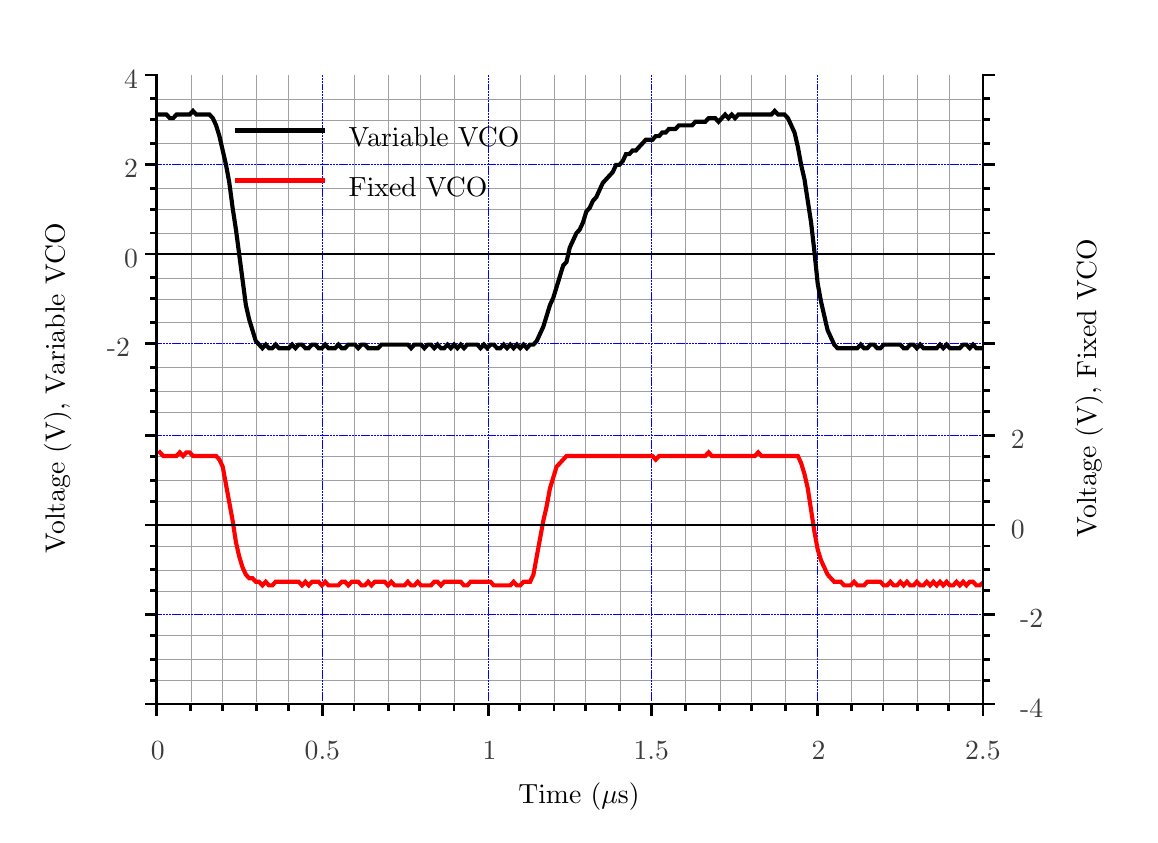
\begin{tikzpicture}{0pt}{0pt}{419pt}{299pt}
	\clip(0pt,299pt) -- (398.436pt,299pt) -- (398.436pt,14.6746pt) -- (0pt,14.6746pt) -- (0pt,299pt);
\begin{scope}
	\clip(46.5951pt,281.883pt) -- (345.184pt,281.883pt) -- (345.184pt,54.6133pt) -- (46.5951pt,54.6133pt) -- (46.5951pt,281.883pt);
	\color[rgb]{0.627451,0.627451,0.643137}
	\draw[line width=0.1pt, dash pattern=on 0.0024cm off 0.008cm, dash phase=0pt, line join=bevel, line cap=rect](58.9571pt,281.883pt) -- (58.9571pt,55.5642pt);
	\color[rgb]{0.627451,0.627451,0.643137}
	\draw[line width=0.1pt, dash pattern=on 0.0024cm off 0.008cm, dash phase=0pt, line join=bevel, line cap=rect](70.3682pt,281.883pt) -- (70.3682pt,55.5642pt);
	\draw[line width=0.1pt, dash pattern=on 0.0024cm off 0.008cm, dash phase=0pt, line join=bevel, line cap=rect](82.7301pt,281.883pt) -- (82.7301pt,55.5642pt);
	\draw[line width=0.1pt, dash pattern=on 0.0024cm off 0.008cm, dash phase=0pt, line join=bevel, line cap=rect](94.1412pt,281.883pt) -- (94.1412pt,55.5642pt);
	\draw[line width=0.1pt, dash pattern=on 0.0024cm off 0.008cm, dash phase=0pt, line join=bevel, line cap=rect](117.914pt,281.883pt) -- (117.914pt,55.5642pt);
	\draw[line width=0.1pt, dash pattern=on 0.0024cm off 0.008cm, dash phase=0pt, line join=bevel, line cap=rect](130.276pt,281.883pt) -- (130.276pt,55.5642pt);
	\draw[line width=0.1pt, dash pattern=on 0.0024cm off 0.008cm, dash phase=0pt, line join=bevel, line cap=rect](141.687pt,281.883pt) -- (141.687pt,55.5642pt);
	\draw[line width=0.1pt, dash pattern=on 0.0024cm off 0.008cm, dash phase=0pt, line join=bevel, line cap=rect](154.049pt,281.883pt) -- (154.049pt,55.5642pt);
	\draw[line width=0.1pt, dash pattern=on 0.0024cm off 0.008cm, dash phase=0pt, line join=bevel, line cap=rect](177.822pt,281.883pt) -- (177.822pt,55.5642pt);
	\draw[line width=0.1pt, dash pattern=on 0.0024cm off 0.008cm, dash phase=0pt, line join=bevel, line cap=rect](190.184pt,281.883pt) -- (190.184pt,55.5642pt);
	\draw[line width=0.1pt, dash pattern=on 0.0024cm off 0.008cm, dash phase=0pt, line join=bevel, line cap=rect](201.595pt,281.883pt) -- (201.595pt,55.5642pt);
	\draw[line width=0.1pt, dash pattern=on 0.0024cm off 0.008cm, dash phase=0pt, line join=bevel, line cap=rect](213.957pt,281.883pt) -- (213.957pt,55.5642pt);
	\draw[line width=0.1pt, dash pattern=on 0.0024cm off 0.008cm, dash phase=0pt, line join=bevel, line cap=rect](237.73pt,281.883pt) -- (237.73pt,55.5642pt);
	\draw[line width=0.1pt, dash pattern=on 0.0024cm off 0.008cm, dash phase=0pt, line join=bevel, line cap=rect](250.092pt,281.883pt) -- (250.092pt,55.5642pt);
	\draw[line width=0.1pt, dash pattern=on 0.0024cm off 0.008cm, dash phase=0pt, line join=bevel, line cap=rect](261.503pt,281.883pt) -- (261.503pt,55.5642pt);
	\draw[line width=0.1pt, dash pattern=on 0.0024cm off 0.008cm, dash phase=0pt, line join=bevel, line cap=rect](273.865pt,281.883pt) -- (273.865pt,55.5642pt);
	\draw[line width=0.1pt, dash pattern=on 0.0024cm off 0.008cm, dash phase=0pt, line join=bevel, line cap=rect](297.638pt,281.883pt) -- (297.638pt,55.5642pt);
	\draw[line width=0.1pt, dash pattern=on 0.0024cm off 0.008cm, dash phase=0pt, line join=bevel, line cap=rect](309.049pt,281.883pt) -- (309.049pt,55.5642pt);
	\draw[line width=0.1pt, dash pattern=on 0.0024cm off 0.008cm, dash phase=0pt, line join=bevel, line cap=rect](321.411pt,281.883pt) -- (321.411pt,55.5642pt);
	\draw[line width=0.1pt, dash pattern=on 0.0024cm off 0.008cm, dash phase=0pt, line join=bevel, line cap=rect](332.822pt,281.883pt) -- (332.822pt,55.5642pt);
	\draw[line width=0.1pt, dash pattern=on 0.0024cm off 0.008cm, dash phase=0pt, line join=bevel, line cap=rect](46.5951pt,63.1716pt) -- (344.233pt,63.1716pt);
	\draw[line width=0.1pt, dash pattern=on 0.0024cm off 0.008cm, dash phase=0pt, line join=bevel, line cap=rect](46.5951pt,79.3372pt) -- (344.233pt,79.3372pt);
	\draw[line width=0.1pt, dash pattern=on 0.0024cm off 0.008cm, dash phase=0pt, line join=bevel, line cap=rect](46.5951pt,95.5029pt) -- (344.233pt,95.5029pt);
	\draw[line width=0.1pt, dash pattern=on 0.0024cm off 0.008cm, dash phase=0pt, line join=bevel, line cap=rect](46.5951pt,111.669pt) -- (344.233pt,111.669pt);
	\draw[line width=0.1pt, dash pattern=on 0.0024cm off 0.008cm, dash phase=0pt, line join=bevel, line cap=rect](46.5951pt,127.834pt) -- (344.233pt,127.834pt);
	\draw[line width=0.1pt, dash pattern=on 0.0024cm off 0.008cm, dash phase=0pt, line join=bevel, line cap=rect](46.5951pt,144pt) -- (344.233pt,144pt);
	\draw[line width=0.1pt, dash pattern=on 0.0024cm off 0.008cm, dash phase=0pt, line join=bevel, line cap=rect](46.5951pt,160.166pt) -- (344.233pt,160.166pt);
	\draw[line width=0.1pt, dash pattern=on 0.0024cm off 0.008cm, dash phase=0pt, line join=bevel, line cap=rect](46.5951pt,176.331pt) -- (344.233pt,176.331pt);
	\draw[line width=0.1pt, dash pattern=on 0.0024cm off 0.008cm, dash phase=0pt, line join=bevel, line cap=rect](46.5951pt,192.497pt) -- (344.233pt,192.497pt);
	\draw[line width=0.1pt, dash pattern=on 0.0024cm off 0.008cm, dash phase=0pt, line join=bevel, line cap=rect](46.5951pt,208.662pt) -- (344.233pt,208.662pt);
	\draw[line width=0.1pt, dash pattern=on 0.0024cm off 0.008cm, dash phase=0pt, line join=bevel, line cap=rect](46.5951pt,224.828pt) -- (344.233pt,224.828pt);
	\draw[line width=0.1pt, dash pattern=on 0.0024cm off 0.008cm, dash phase=0pt, line join=bevel, line cap=rect](46.5951pt,240.994pt) -- (344.233pt,240.994pt);
	\draw[line width=0.1pt, dash pattern=on 0.0024cm off 0.008cm, dash phase=0pt, line join=bevel, line cap=rect](46.5951pt,257.159pt) -- (344.233pt,257.159pt);
	\draw[line width=0.1pt, dash pattern=on 0.0024cm off 0.008cm, dash phase=0pt, line join=bevel, line cap=rect](46.5951pt,273.325pt) -- (344.233pt,273.325pt);
	\draw[line width=0.1pt, dash pattern=on 0.0024cm off 0.008cm, dash phase=0pt, line join=bevel, line cap=rect](46.5951pt,70.7789pt) -- (344.233pt,70.7789pt);
	\draw[line width=0.1pt, dash pattern=on 0.0024cm off 0.008cm, dash phase=0pt, line join=bevel, line cap=rect](46.5951pt,103.11pt) -- (344.233pt,103.11pt);
	\draw[line width=0.1pt, dash pattern=on 0.0024cm off 0.008cm, dash phase=0pt, line join=bevel, line cap=rect](46.5951pt,135.442pt) -- (344.233pt,135.442pt);
	\draw[line width=0.1pt, dash pattern=on 0.0024cm off 0.008cm, dash phase=0pt, line join=bevel, line cap=rect](46.5951pt,167.773pt) -- (344.233pt,167.773pt);
	\draw[line width=0.1pt, dash pattern=on 0.0024cm off 0.008cm, dash phase=0pt, line join=bevel, line cap=rect](46.5951pt,201.055pt) -- (344.233pt,201.055pt);
	\draw[line width=0.1pt, dash pattern=on 0.0024cm off 0.008cm, dash phase=0pt, line join=bevel, line cap=rect](46.5951pt,233.386pt) -- (344.233pt,233.386pt);
	\draw[line width=0.1pt, dash pattern=on 0.0024cm off 0.008cm, dash phase=0pt, line join=bevel, line cap=rect](46.5951pt,265.718pt) -- (344.233pt,265.718pt);
	\color[rgb]{0,0,1}
	\draw[line width=0.2pt, dash pattern=on 0.024cm off 0.016cm, dash phase=0pt, line join=bevel, line cap=rect](106.503pt,281.883pt) -- (106.503pt,55.5642pt);
	\draw[line width=0.2pt, dash pattern=on 0.024cm off 0.016cm, dash phase=0pt, line join=bevel, line cap=rect](166.411pt,281.883pt) -- (166.411pt,55.5642pt);
	\draw[line width=0.2pt, dash pattern=on 0.024cm off 0.016cm, dash phase=0pt, line join=bevel, line cap=rect](225.368pt,281.883pt) -- (225.368pt,55.5642pt);
	\draw[line width=0.2pt, dash pattern=on 0.024cm off 0.016cm, dash phase=0pt, line join=bevel, line cap=rect](285.276pt,281.883pt) -- (285.276pt,55.5642pt);
	\draw[line width=0.2pt, dash pattern=on 0.024cm off 0.016cm, dash phase=0pt, line join=bevel, line cap=rect](46.5951pt,86.9446pt) -- (344.233pt,86.9446pt);
	\draw[line width=0.2pt, dash pattern=on 0.024cm off 0.016cm, dash phase=0pt, line join=bevel, line cap=rect](46.5951pt,119.276pt) -- (344.233pt,119.276pt);
	\draw[line width=0.2pt, dash pattern=on 0.024cm off 0.016cm, dash phase=0pt, line join=bevel, line cap=rect](46.5951pt,151.607pt) -- (344.233pt,151.607pt);
	\draw[line width=0.2pt, dash pattern=on 0.024cm off 0.016cm, dash phase=0pt, line join=bevel, line cap=rect](46.5951pt,184.889pt) -- (344.233pt,184.889pt);
	\draw[line width=0.2pt, dash pattern=on 0.024cm off 0.016cm, dash phase=0pt, line join=bevel, line cap=rect](46.5951pt,217.221pt) -- (344.233pt,217.221pt);
	\draw[line width=0.2pt, dash pattern=on 0.024cm off 0.016cm, dash phase=0pt, line join=bevel, line cap=rect](46.5951pt,249.552pt) -- (344.233pt,249.552pt);
	\color[rgb]{0,0,0}
	\draw[line width=1.5pt, line join=miter, line cap=rect](47.7895pt,267.598pt) -- (48.9838pt,267.598pt) -- (50.1782pt,267.598pt) -- (51.3726pt,266.299pt) -- (52.5669pt,266.299pt) -- (53.7613pt,267.598pt) -- (54.9556pt,267.598pt) -- (56.15pt,267.598pt) -- (57.3443pt,267.598pt) -- (58.5387pt,267.598pt) -- (59.7331pt,268.897pt) -- (60.9274pt,267.598pt) -- (62.1218pt,267.598pt) -- (63.3161pt,267.598pt) -- (64.5105pt,267.598pt) -- (65.7048pt,267.598pt) -- (66.8992pt,266.299pt) -- (68.0936pt,263.702pt) -- (69.2879pt,259.806pt) -- (70.4823pt,254.611pt) -- (71.6766pt,249.416pt) -- (72.871pt,242.923pt) -- (74.0653pt,233.832pt) -- (75.2597pt,226.04pt) -- (76.4541pt,216.949pt) -- (77.6484pt,207.858pt) -- (78.8428pt,198.767pt) -- (80.0371pt,193.573pt) -- (81.2315pt,189.677pt) -- (82.4258pt,185.781pt) -- (83.6202pt,184.482pt) -- (84.8146pt,183.183pt) -- (86.0089pt,184.482pt) -- (87.2033pt,183.183pt) -- (88.3976pt,183.183pt) -- (89.592pt,184.482pt) -- (90.7863pt,183.183pt) -- (91.9807pt,183.183pt) -- (93.175pt,183.183pt) -- (94.3694pt,183.183pt) -- (95.5638pt,184.482pt) -- (96.7581pt,183.183pt) -- (97.9525pt,184.482pt) -- (99.1468pt,184.482pt) -- (100.341pt,183.183pt) -- (101.536pt,183.183pt) -- (102.73pt,184.482pt) -- (103.924pt,184.482pt) -- (105.119pt,183.183pt) -- (106.313pt,183.183pt) -- (107.507pt,184.482pt) -- (108.702pt,183.183pt) -- (109.896pt,183.183pt) -- (111.09pt,183.183pt) -- (112.285pt,184.482pt) -- (113.479pt,183.183pt) -- (114.673pt,183.183pt) -- (115.868pt,184.482pt) -- (117.062pt,184.482pt) -- (118.257pt,184.482pt) -- (119.451pt,183.183pt) -- (120.645pt,184.482pt) -- (121.84pt,184.482pt) -- (123.034pt,183.183pt) -- (124.228pt,183.183pt) -- (125.423pt,183.183pt) -- (126.617pt,183.183pt) -- (127.811pt,184.482pt) -- (129.006pt,184.482pt) -- (130.2pt,184.482pt) -- (131.394pt,184.482pt) -- (132.589pt,184.482pt) -- (133.783pt,184.482pt) -- (134.978pt,184.482pt) -- (136.172pt,184.482pt) -- (137.366pt,184.482pt) -- (138.561pt,183.183pt) -- (139.755pt,184.482pt) -- (140.949pt,184.482pt) -- (142.144pt,184.482pt) -- (143.338pt,183.183pt) -- (144.532pt,184.482pt) -- (145.727pt,184.482pt) -- (146.921pt,183.183pt) -- (148.115pt,184.482pt) -- (149.31pt,183.183pt) -- (150.504pt,183.183pt) -- (151.699pt,184.482pt) -- (152.893pt,183.183pt) -- (154.087pt,184.482pt) -- (155.282pt,183.183pt) -- (156.476pt,184.482pt) -- (157.67pt,183.183pt) -- (158.865pt,184.482pt) -- (160.059pt,184.482pt) -- (161.253pt,184.482pt) -- (162.448pt,184.482pt) -- (163.642pt,183.183pt) -- (164.836pt,184.482pt) -- (166.031pt,183.183pt) -- (167.225pt,184.482pt) -- (168.42pt,184.482pt) -- (169.614pt,183.183pt) -- (170.808pt,183.183pt) -- (172.003pt,184.482pt) -- (173.197pt,183.183pt) -- (174.391pt,184.482pt) -- (175.586pt,183.183pt) -- (176.78pt,184.482pt) -- (177.974pt,183.183pt) -- (179.169pt,184.482pt) -- (180.363pt,183.183pt) -- (181.557pt,184.482pt) -- (182.752pt,184.482pt) -- (183.946pt,185.781pt) -- (185.141pt,188.378pt) -- (186.335pt,190.975pt) -- (187.529pt,194.871pt) -- (188.724pt,198.767pt) -- (189.918pt,201.365pt) -- (191.112pt,205.261pt) -- (192.307pt,209.157pt) -- (193.501pt,213.053pt) -- (194.695pt,214.352pt) -- (195.89pt,219.546pt) -- (197.084pt,222.144pt) -- (198.278pt,224.741pt) -- (199.473pt,226.04pt) -- (200.667pt,228.637pt) -- (201.862pt,232.533pt) -- (203.056pt,233.832pt) -- (204.25pt,236.429pt) -- (205.445pt,237.728pt) -- (206.639pt,240.325pt) -- (207.833pt,242.923pt) -- (209.028pt,244.222pt) -- (210.222pt,245.52pt) -- (211.416pt,246.819pt) -- (212.611pt,249.416pt) -- (213.805pt,249.416pt) -- (214.999pt,250.715pt) -- (216.194pt,253.312pt) -- (217.388pt,253.312pt) -- (218.583pt,254.611pt) -- (219.777pt,254.611pt) -- (220.971pt,255.91pt) -- (222.166pt,257.208pt) -- (223.36pt,258.507pt) -- (224.554pt,258.507pt) -- (225.749pt,258.507pt) -- (226.943pt,259.806pt) -- (228.137pt,259.806pt) -- (229.332pt,261.104pt) -- (230.526pt,261.104pt) -- (231.72pt,262.403pt) -- (232.915pt,262.403pt) -- (234.109pt,262.403pt) -- (235.304pt,263.702pt) -- (236.498pt,263.702pt) -- (237.692pt,263.702pt) -- (238.887pt,263.702pt) -- (240.081pt,263.702pt) -- (241.275pt,265pt) -- (242.47pt,265pt) -- (243.664pt,265pt) -- (244.858pt,265pt) -- (246.053pt,266.299pt) -- (247.247pt,266.299pt) -- (248.441pt,266.299pt) -- (249.636pt,265pt) -- (250.83pt,266.299pt) -- (252.025pt,267.598pt) -- (253.219pt,266.299pt) -- (254.413pt,267.598pt) -- (255.608pt,266.299pt) -- (256.802pt,267.598pt) -- (257.996pt,267.598pt) -- (259.191pt,267.598pt) -- (260.385pt,267.598pt) -- (261.579pt,267.598pt) -- (262.774pt,267.598pt) -- (263.968pt,267.598pt) -- (265.162pt,267.598pt) -- (266.357pt,267.598pt) -- (267.551pt,267.598pt) -- (268.746pt,267.598pt) -- (269.94pt,268.897pt) -- (271.134pt,267.598pt) -- (272.329pt,267.598pt) -- (273.523pt,267.598pt) -- (274.717pt,266.299pt) -- (275.912pt,263.702pt) -- (277.106pt,261.104pt) -- (278.3pt,255.91pt) -- (279.495pt,249.416pt) -- (280.689pt,244.222pt) -- (281.883pt,236.429pt) -- (283.078pt,228.637pt) -- (284.272pt,218.248pt) -- (285.466pt,206.56pt) -- (286.661pt,200.066pt) -- (287.855pt,194.871pt) -- (289.05pt,189.677pt) -- (290.244pt,187.079pt) -- (291.438pt,184.482pt) -- (292.633pt,183.183pt) -- (293.827pt,183.183pt) -- (295.021pt,183.183pt) -- (296.216pt,183.183pt) -- (297.41pt,183.183pt) -- (298.604pt,183.183pt) -- (299.799pt,183.183pt) -- (300.993pt,184.482pt) -- (302.187pt,183.183pt) -- (303.382pt,183.183pt) -- (304.576pt,184.482pt) -- (305.771pt,184.482pt) -- (306.965pt,183.183pt) -- (308.159pt,183.183pt) -- (309.354pt,184.482pt) -- (310.548pt,184.482pt) -- (311.742pt,184.482pt) -- (312.937pt,184.482pt) -- (314.131pt,184.482pt) -- (315.325pt,184.482pt) -- (316.52pt,183.183pt) -- (317.714pt,183.183pt) -- (318.908pt,184.482pt) -- (320.103pt,184.482pt) -- (321.297pt,183.183pt) -- (322.492pt,184.482pt) -- (323.686pt,183.183pt) -- (324.88pt,183.183pt) -- (326.075pt,183.183pt) -- (327.269pt,183.183pt) -- (328.463pt,183.183pt) -- (329.658pt,184.482pt) -- (330.852pt,183.183pt) -- (332.046pt,184.482pt) -- (333.241pt,183.183pt) -- (334.435pt,183.183pt) -- (335.629pt,183.183pt) -- (336.824pt,183.183pt) -- (338.018pt,184.482pt) -- (339.213pt,184.482pt) -- (340.407pt,183.183pt) -- (341.601pt,184.482pt) -- (342.796pt,183.183pt) -- (343.99pt,183.183pt) -- (345.184pt,183.183pt);
	\color[rgb]{1,0,0}
	\draw[line width=1.5pt, line join=miter, line cap=rect](47.7895pt,145.521pt) -- (48.9838pt,144.223pt) -- (50.1782pt,144.223pt) -- (51.3726pt,144.223pt) -- (52.5669pt,144.223pt) -- (53.7613pt,144.223pt) -- (54.9556pt,145.521pt) -- (56.15pt,144.223pt) -- (57.3443pt,145.521pt) -- (58.5387pt,145.521pt) -- (59.7331pt,144.223pt) -- (60.9274pt,144.223pt) -- (62.1218pt,144.223pt) -- (63.3161pt,144.223pt) -- (64.5105pt,144.223pt) -- (65.7048pt,144.223pt) -- (66.8992pt,144.223pt) -- (68.0936pt,144.223pt) -- (69.2879pt,142.924pt) -- (70.4823pt,140.327pt) -- (71.6766pt,133.833pt) -- (72.871pt,127.34pt) -- (74.0653pt,120.846pt) -- (75.2597pt,113.054pt) -- (76.4541pt,107.859pt) -- (77.6484pt,103.963pt) -- (78.8428pt,101.366pt) -- (80.0371pt,100.067pt) -- (81.2315pt,100.067pt) -- (82.4258pt,98.7686pt) -- (83.6202pt,98.7686pt) -- (84.8146pt,97.4699pt) -- (86.0089pt,98.7686pt) -- (87.2033pt,97.4699pt) -- (88.3976pt,97.4699pt) -- (89.592pt,98.7686pt) -- (90.7863pt,98.7686pt) -- (91.9807pt,98.7686pt) -- (93.175pt,98.7686pt) -- (94.3694pt,98.7686pt) -- (95.5638pt,98.7686pt) -- (96.7581pt,98.7686pt) -- (97.9525pt,98.7686pt) -- (99.1468pt,97.4699pt) -- (100.341pt,98.7686pt) -- (101.536pt,97.4699pt) -- (102.73pt,98.7686pt) -- (103.924pt,98.7686pt) -- (105.119pt,98.7686pt) -- (106.313pt,97.4699pt) -- (107.507pt,98.7686pt) -- (108.702pt,97.4699pt) -- (109.896pt,97.4699pt) -- (111.09pt,97.4699pt) -- (112.285pt,97.4699pt) -- (113.479pt,98.7686pt) -- (114.673pt,98.7686pt) -- (115.868pt,97.4699pt) -- (117.062pt,98.7686pt) -- (118.257pt,98.7686pt) -- (119.451pt,98.7686pt) -- (120.645pt,97.4699pt) -- (121.84pt,97.4699pt) -- (123.034pt,98.7686pt) -- (124.228pt,97.4699pt) -- (125.423pt,98.7686pt) -- (126.617pt,98.7686pt) -- (127.811pt,98.7686pt) -- (129.006pt,98.7686pt) -- (130.2pt,97.4699pt) -- (131.394pt,98.7686pt) -- (132.589pt,97.4699pt) -- (133.783pt,97.4699pt) -- (134.978pt,97.4699pt) -- (136.172pt,97.4699pt) -- (137.366pt,98.7686pt) -- (138.561pt,97.4699pt) -- (139.755pt,97.4699pt) -- (140.949pt,98.7686pt) -- (142.144pt,97.4699pt) -- (143.338pt,97.4699pt) -- (144.532pt,97.4699pt) -- (145.727pt,97.4699pt) -- (146.921pt,98.7686pt) -- (148.115pt,98.7686pt) -- (149.31pt,97.4699pt) -- (150.504pt,98.7686pt) -- (151.699pt,98.7686pt) -- (152.893pt,98.7686pt) -- (154.087pt,98.7686pt) -- (155.282pt,98.7686pt) -- (156.476pt,98.7686pt) -- (157.67pt,97.4699pt) -- (158.865pt,97.4699pt) -- (160.059pt,98.7686pt) -- (161.253pt,98.7686pt) -- (162.448pt,98.7686pt) -- (163.642pt,98.7686pt) -- (164.836pt,98.7686pt) -- (166.031pt,98.7686pt) -- (167.225pt,98.7686pt) -- (168.42pt,97.4699pt) -- (169.614pt,97.4699pt) -- (170.808pt,97.4699pt) -- (172.003pt,97.4699pt) -- (173.197pt,97.4699pt) -- (174.391pt,97.4699pt) -- (175.586pt,98.7686pt) -- (176.78pt,97.4699pt) -- (177.974pt,97.4699pt) -- (179.169pt,98.7686pt) -- (180.363pt,98.7686pt) -- (181.557pt,98.7686pt) -- (182.752pt,101.366pt) -- (183.946pt,107.859pt) -- (185.141pt,114.353pt) -- (186.335pt,120.846pt) -- (187.529pt,126.041pt) -- (188.724pt,132.534pt) -- (189.918pt,136.431pt) -- (191.112pt,140.327pt) -- (192.307pt,141.625pt) -- (193.501pt,142.924pt) -- (194.695pt,144.223pt) -- (195.89pt,144.223pt) -- (197.084pt,144.223pt) -- (198.278pt,144.223pt) -- (199.473pt,144.223pt) -- (200.667pt,144.223pt) -- (201.862pt,144.223pt) -- (203.056pt,144.223pt) -- (204.25pt,144.223pt) -- (205.445pt,144.223pt) -- (206.639pt,144.223pt) -- (207.833pt,144.223pt) -- (209.028pt,144.223pt) -- (210.222pt,144.223pt) -- (211.416pt,144.223pt) -- (212.611pt,144.223pt) -- (213.805pt,144.223pt) -- (214.999pt,144.223pt) -- (216.194pt,144.223pt) -- (217.388pt,144.223pt) -- (218.583pt,144.223pt) -- (219.777pt,144.223pt) -- (220.971pt,144.223pt) -- (222.166pt,144.223pt) -- (223.36pt,144.223pt) -- (224.554pt,144.223pt) -- (225.749pt,144.223pt) -- (226.943pt,142.924pt) -- (228.137pt,144.223pt) -- (229.332pt,144.223pt) -- (230.526pt,144.223pt) -- (231.72pt,144.223pt) -- (232.915pt,144.223pt) -- (234.109pt,144.223pt) -- (235.304pt,144.223pt) -- (236.498pt,144.223pt) -- (237.692pt,144.223pt) -- (238.887pt,144.223pt) -- (240.081pt,144.223pt) -- (241.275pt,144.223pt) -- (242.47pt,144.223pt) -- (243.664pt,144.223pt) -- (244.858pt,144.223pt) -- (246.053pt,145.521pt) -- (247.247pt,144.223pt) -- (248.441pt,144.223pt) -- (249.636pt,144.223pt) -- (250.83pt,144.223pt) -- (252.025pt,144.223pt) -- (253.219pt,144.223pt) -- (254.413pt,144.223pt) -- (255.608pt,144.223pt) -- (256.802pt,144.223pt) -- (257.996pt,144.223pt) -- (259.191pt,144.223pt) -- (260.385pt,144.223pt) -- (261.579pt,144.223pt) -- (262.774pt,144.223pt) -- (263.968pt,145.521pt) -- (265.162pt,144.223pt) -- (266.357pt,144.223pt) -- (267.551pt,144.223pt) -- (268.746pt,144.223pt) -- (269.94pt,144.223pt) -- (271.134pt,144.223pt) -- (272.329pt,144.223pt) -- (273.523pt,144.223pt) -- (274.717pt,144.223pt) -- (275.912pt,144.223pt) -- (277.106pt,144.223pt) -- (278.3pt,144.223pt) -- (279.495pt,141.625pt) -- (280.689pt,137.729pt) -- (281.883pt,132.534pt) -- (283.078pt,124.742pt) -- (284.272pt,116.95pt) -- (285.466pt,110.457pt) -- (286.661pt,106.561pt) -- (287.855pt,103.963pt) -- (289.05pt,101.366pt) -- (290.244pt,100.067pt) -- (291.438pt,98.7686pt) -- (292.633pt,98.7686pt) -- (293.827pt,98.7686pt) -- (295.021pt,97.4699pt) -- (296.216pt,97.4699pt) -- (297.41pt,97.4699pt) -- (298.604pt,98.7686pt) -- (299.799pt,97.4699pt) -- (300.993pt,97.4699pt) -- (302.187pt,97.4699pt) -- (303.382pt,98.7686pt) -- (304.576pt,98.7686pt) -- (305.771pt,98.7686pt) -- (306.965pt,98.7686pt) -- (308.159pt,98.7686pt) -- (309.354pt,97.4699pt) -- (310.548pt,97.4699pt) -- (311.742pt,98.7686pt) -- (312.937pt,97.4699pt) -- (314.131pt,97.4699pt) -- (315.325pt,98.7686pt) -- (316.52pt,97.4699pt) -- (317.714pt,98.7686pt) -- (318.908pt,97.4699pt) -- (320.103pt,97.4699pt) -- (321.297pt,98.7686pt) -- (322.492pt,97.4699pt) -- (323.686pt,97.4699pt) -- (324.88pt,98.7686pt) -- (326.075pt,97.4699pt) -- (327.269pt,98.7686pt) -- (328.463pt,97.4699pt) -- (329.658pt,98.7686pt) -- (330.852pt,97.4699pt) -- (332.046pt,98.7686pt) -- (333.241pt,97.4699pt) -- (334.435pt,97.4699pt) -- (335.629pt,98.7686pt) -- (336.824pt,97.4699pt) -- (338.018pt,98.7686pt) -- (339.213pt,97.4699pt) -- (340.407pt,98.7686pt) -- (341.601pt,98.7686pt) -- (342.796pt,97.4699pt) -- (343.99pt,97.4699pt) -- (345.184pt,98.4209pt);
	\color[rgb]{0,0,0}
	\draw[line width=1pt, line join=bevel, line cap=rect](46.5951pt,217.221pt) -- (344.233pt,217.221pt);
	\draw[line width=1pt, line join=miter, line cap=rect](46.5951pt,119.276pt) -- (345.184pt,119.276pt);
\end{scope}
\begin{scope}
	\color[rgb]{0,0,0}
	\pgftext[center, base, at={\pgfpoint{13.3129pt}{168.716pt}},rotate=90]{Voltage (V), Variable VCO}
	\color[rgb]{0.235294,0.235294,0.235294}

	\pgftext[center, base, at={\pgfpoint{32.8216pt}{180.135pt}}]{-2}
	\pgftext[center, base, at={\pgfpoint{37.3311pt}{212.466pt}}]{0}
	\pgftext[center, base, at={\pgfpoint{37.3311pt}{244.798pt}}]{2}
	\pgftext[center, base, at={\pgfpoint{37.3311pt}{277.129pt}}]{4}
	\color[rgb]{0,0,0}
	\draw[line width=1pt, line join=bevel, line cap=rect](46.5951pt,63.1716pt) -- (44.6933pt,63.1716pt);
	\draw[line width=1pt, line join=bevel, line cap=rect](46.5951pt,79.3372pt) -- (44.6933pt,79.3372pt);
	\draw[line width=1pt, line join=bevel, line cap=rect](46.5951pt,95.5029pt) -- (44.6933pt,95.5029pt);
	\draw[line width=1pt, line join=bevel, line cap=rect](46.5951pt,111.669pt) -- (44.6933pt,111.669pt);
	\draw[line width=1pt, line join=bevel, line cap=rect](46.5951pt,127.834pt) -- (44.6933pt,127.834pt);
	\draw[line width=1pt, line join=bevel, line cap=rect](46.5951pt,144pt) -- (44.6933pt,144pt);
	\draw[line width=1pt, line join=bevel, line cap=rect](46.5951pt,160.166pt) -- (44.6933pt,160.166pt);
	\draw[line width=1pt, line join=bevel, line cap=rect](46.5951pt,176.331pt) -- (44.6933pt,176.331pt);
	\draw[line width=1pt, line join=bevel, line cap=rect](46.5951pt,192.497pt) -- (44.6933pt,192.497pt);
	\draw[line width=1pt, line join=bevel, line cap=rect](46.5951pt,208.662pt) -- (44.6933pt,208.662pt);
	\draw[line width=1pt, line join=bevel, line cap=rect](46.5951pt,224.828pt) -- (44.6933pt,224.828pt);
	\draw[line width=1pt, line join=bevel, line cap=rect](46.5951pt,240.994pt) -- (44.6933pt,240.994pt);
	\draw[line width=1pt, line join=bevel, line cap=rect](46.5951pt,257.159pt) -- (44.6933pt,257.159pt);
	\draw[line width=1pt, line join=bevel, line cap=rect](46.5951pt,273.325pt) -- (44.6933pt,273.325pt);
	\draw[line width=1pt, line join=bevel, line cap=rect](46.5951pt,70.7789pt) -- (44.6933pt,70.7789pt);
	\draw[line width=1pt, line join=bevel, line cap=rect](46.5951pt,103.11pt) -- (44.6933pt,103.11pt);
	\draw[line width=1pt, line join=bevel, line cap=rect](46.5951pt,135.442pt) -- (44.6933pt,135.442pt);
	\draw[line width=1pt, line join=bevel, line cap=rect](46.5951pt,167.773pt) -- (44.6933pt,167.773pt);
	\draw[line width=1pt, line join=bevel, line cap=rect](46.5951pt,201.055pt) -- (44.6933pt,201.055pt);
	\draw[line width=1pt, line join=bevel, line cap=rect](46.5951pt,233.386pt) -- (44.6933pt,233.386pt);
	\draw[line width=1pt, line join=bevel, line cap=rect](46.5951pt,265.718pt) -- (44.6933pt,265.718pt);
	\draw[line width=1pt, line join=bevel, line cap=rect](46.5951pt,54.6133pt) -- (42.7914pt,54.6133pt);
	\draw[line width=1pt, line join=bevel, line cap=rect](46.5951pt,86.9446pt) -- (42.7914pt,86.9446pt);
	\draw[line width=1pt, line join=bevel, line cap=rect](46.5951pt,119.276pt) -- (42.7914pt,119.276pt);
	\draw[line width=1pt, line join=bevel, line cap=rect](46.5951pt,151.607pt) -- (42.7914pt,151.607pt);
	\draw[line width=1pt, line join=bevel, line cap=rect](46.5951pt,184.889pt) -- (42.7914pt,184.889pt);
	\draw[line width=1pt, line join=bevel, line cap=rect](46.5951pt,217.221pt) -- (42.7914pt,217.221pt);
	\draw[line width=1pt, line join=bevel, line cap=rect](46.5951pt,249.552pt) -- (42.7914pt,249.552pt);
	\draw[line width=1pt, line join=bevel, line cap=rect](46.5951pt,281.883pt) -- (42.7914pt,281.883pt);
	\draw[line width=1pt, line join=bevel, line cap=rect](46.5951pt,281.883pt) -- (46.5951pt,54.6133pt);
	\pgftext[center, base, at={\pgfpoint{386.074pt}{168.724pt}},rotate=90]{Voltage (V), Fixed VCO}
	\color[rgb]{0.235294,0.235294,0.235294}
	\pgftext[center, base, at={\pgfpoint{362.791pt}{49.8587pt}}]{-4}
	\pgftext[center, base, at={\pgfpoint{362.791pt}{82.19pt}}]{-2}
	\pgftext[center, base, at={\pgfpoint{357.791pt}{114.521pt}}]{0}
	\pgftext[center, base, at={\pgfpoint{357.791pt}{146.853pt}}]{2}

	\color[rgb]{0,0,0}
	\draw[line width=1pt, line join=bevel, line cap=rect](345.184pt,63.1716pt) -- (347.086pt,63.1716pt);
	\draw[line width=1pt, line join=bevel, line cap=rect](345.184pt,79.3372pt) -- (347.086pt,79.3372pt);
	\draw[line width=1pt, line join=bevel, line cap=rect](345.184pt,95.5029pt) -- (347.086pt,95.5029pt);
	\draw[line width=1pt, line join=bevel, line cap=rect](345.184pt,111.669pt) -- (347.086pt,111.669pt);
	\draw[line width=1pt, line join=bevel, line cap=rect](345.184pt,127.834pt) -- (347.086pt,127.834pt);
	\draw[line width=1pt, line join=bevel, line cap=rect](345.184pt,144pt) -- (347.086pt,144pt);
	\draw[line width=1pt, line join=bevel, line cap=rect](345.184pt,160.166pt) -- (347.086pt,160.166pt);
	\draw[line width=1pt, line join=bevel, line cap=rect](345.184pt,176.331pt) -- (347.086pt,176.331pt);
	\draw[line width=1pt, line join=bevel, line cap=rect](345.184pt,192.497pt) -- (347.086pt,192.497pt);
	\draw[line width=1pt, line join=bevel, line cap=rect](345.184pt,208.662pt) -- (347.086pt,208.662pt);
	\draw[line width=1pt, line join=bevel, line cap=rect](345.184pt,224.828pt) -- (347.086pt,224.828pt);
	\draw[line width=1pt, line join=bevel, line cap=rect](345.184pt,240.994pt) -- (347.086pt,240.994pt);
	\draw[line width=1pt, line join=bevel, line cap=rect](345.184pt,257.159pt) -- (347.086pt,257.159pt);
	\draw[line width=1pt, line join=bevel, line cap=rect](345.184pt,273.325pt) -- (347.086pt,273.325pt);
	\draw[line width=1pt, line join=bevel, line cap=rect](345.184pt,70.7789pt) -- (347.086pt,70.7789pt);
	\draw[line width=1pt, line join=bevel, line cap=rect](345.184pt,103.11pt) -- (347.086pt,103.11pt);
	\draw[line width=1pt, line join=bevel, line cap=rect](345.184pt,135.442pt) -- (347.086pt,135.442pt);
	\draw[line width=1pt, line join=bevel, line cap=rect](345.184pt,167.773pt) -- (347.086pt,167.773pt);
	\draw[line width=1pt, line join=bevel, line cap=rect](345.184pt,201.055pt) -- (347.086pt,201.055pt);
	\draw[line width=1pt, line join=bevel, line cap=rect](345.184pt,233.386pt) -- (347.086pt,233.386pt);
	\draw[line width=1pt, line join=bevel, line cap=rect](345.184pt,265.718pt) -- (347.086pt,265.718pt);
	\draw[line width=1pt, line join=bevel, line cap=rect](345.184pt,54.6133pt) -- (348.988pt,54.6133pt);
	\draw[line width=1pt, line join=bevel, line cap=rect](345.184pt,86.9446pt) -- (348.988pt,86.9446pt);
	\draw[line width=1pt, line join=bevel, line cap=rect](345.184pt,119.276pt) -- (348.988pt,119.276pt);
	\draw[line width=1pt, line join=bevel, line cap=rect](345.184pt,151.607pt) -- (348.988pt,151.607pt);
	\draw[line width=1pt, line join=bevel, line cap=rect](345.184pt,184.889pt) -- (348.988pt,184.889pt);
	\draw[line width=1pt, line join=bevel, line cap=rect](345.184pt,217.221pt) -- (348.988pt,217.221pt);
	\draw[line width=1pt, line join=bevel, line cap=rect](345.184pt,249.552pt) -- (348.988pt,249.552pt);
	\draw[line width=1pt, line join=bevel, line cap=rect](345.184pt,281.883pt) -- (348.988pt,281.883pt);
	\draw[line width=1pt, line join=bevel, line cap=rect](345.184pt,281.883pt) -- (345.184pt,54.6133pt);
	\pgftext[center, base, at={\pgfpoint{199.211pt}{18.4783pt}}]{Time ($\mu$s)}
	\color[rgb]{0.235294,0.235294,0.235294}
	\pgftext[center, base, at={\pgfpoint{47.0632pt}{34.6439pt}}]{0}
	\pgftext[center, base, at={\pgfpoint{106.496pt}{34.6439pt}}]{0.5}
	\pgftext[center, base, at={\pgfpoint{166.879pt}{34.6439pt}}]{1}
	\pgftext[center, base, at={\pgfpoint{225.361pt}{34.6439pt}}]{1.5}
	\pgftext[center, base, at={\pgfpoint{285.744pt}{34.6439pt}}]{2}
	\pgftext[center, base, at={\pgfpoint{345.177pt}{34.6439pt}}]{2.5}
	\color[rgb]{0,0,0}
	\draw[line width=1pt, line join=bevel, line cap=rect](58.9571pt,54.6133pt) -- (58.9571pt,52.7114pt);
	\draw[line width=1pt, line join=bevel, line cap=rect](70.3682pt,54.6133pt) -- (70.3682pt,52.7114pt);
	\draw[line width=1pt, line join=bevel, line cap=rect](82.7301pt,54.6133pt) -- (82.7301pt,52.7114pt);
	\draw[line width=1pt, line join=bevel, line cap=rect](94.1412pt,54.6133pt) -- (94.1412pt,52.7114pt);
	\draw[line width=1pt, line join=bevel, line cap=rect](117.914pt,54.6133pt) -- (117.914pt,52.7114pt);
	\draw[line width=1pt, line join=bevel, line cap=rect](130.276pt,54.6133pt) -- (130.276pt,52.7114pt);
	\draw[line width=1pt, line join=bevel, line cap=rect](141.687pt,54.6133pt) -- (141.687pt,52.7114pt);
	\draw[line width=1pt, line join=bevel, line cap=rect](154.049pt,54.6133pt) -- (154.049pt,52.7114pt);
	\draw[line width=1pt, line join=bevel, line cap=rect](177.822pt,54.6133pt) -- (177.822pt,52.7114pt);
	\draw[line width=1pt, line join=bevel, line cap=rect](190.184pt,54.6133pt) -- (190.184pt,52.7114pt);
	\draw[line width=1pt, line join=bevel, line cap=rect](201.595pt,54.6133pt) -- (201.595pt,52.7114pt);
	\draw[line width=1pt, line join=bevel, line cap=rect](213.957pt,54.6133pt) -- (213.957pt,52.7114pt);
	\draw[line width=1pt, line join=bevel, line cap=rect](237.73pt,54.6133pt) -- (237.73pt,52.7114pt);
	\draw[line width=1pt, line join=bevel, line cap=rect](250.092pt,54.6133pt) -- (250.092pt,52.7114pt);
	\draw[line width=1pt, line join=bevel, line cap=rect](261.503pt,54.6133pt) -- (261.503pt,52.7114pt);
	\draw[line width=1pt, line join=bevel, line cap=rect](273.865pt,54.6133pt) -- (273.865pt,52.7114pt);
	\draw[line width=1pt, line join=bevel, line cap=rect](297.638pt,54.6133pt) -- (297.638pt,52.7114pt);
	\draw[line width=1pt, line join=bevel, line cap=rect](309.049pt,54.6133pt) -- (309.049pt,52.7114pt);
	\draw[line width=1pt, line join=bevel, line cap=rect](321.411pt,54.6133pt) -- (321.411pt,52.7114pt);
	\draw[line width=1pt, line join=bevel, line cap=rect](332.822pt,54.6133pt) -- (332.822pt,52.7114pt);
	\draw[line width=1pt, line join=bevel, line cap=rect](46.5951pt,54.6133pt) -- (46.5951pt,50.8096pt);
	\draw[line width=1pt, line join=bevel, line cap=rect](106.503pt,54.6133pt) -- (106.503pt,50.8096pt);
	\draw[line width=1pt, line join=bevel, line cap=rect](166.411pt,54.6133pt) -- (166.411pt,50.8096pt);
	\draw[line width=1pt, line join=bevel, line cap=rect](225.368pt,54.6133pt) -- (225.368pt,50.8096pt);
	\draw[line width=1pt, line join=bevel, line cap=rect](285.276pt,54.6133pt) -- (285.276pt,50.8096pt);
	\draw[line width=1pt, line join=bevel, line cap=rect](345.184pt,54.6133pt) -- (345.184pt,50.8096pt);
	\draw[line width=1pt, line join=bevel, line cap=rect](46.5951pt,54.6133pt) -- (345.184pt,54.6133pt);
	\draw[line width=2pt, line join=miter, line cap=rect](76.0737pt,261.914pt) -- (106.503pt,261.914pt);
	\pgftext[left, base, at={\pgfpoint{116.012pt}{256.209pt}}]{Variable VCO}
	\color[rgb]{1,0,0}
	\draw[line width=2pt, line join=miter, line cap=rect](76.0737pt,243.847pt) -- (106.503pt,243.847pt);
	\color[rgb]{0,0,0}
	\pgftext[left, base, at={\pgfpoint{116.012pt}{238.141pt}}]{Fixed VCO}
\end{scope}
\end{tikzpicture}

		\caption{The final signal produced by the components of the theremin. The upper signal is the variable VCO, the lower the fixed VCO. They are both input into the mixer.}
		\label{fig:final}
	\end{center}
\end{figure}

\begin{figure}
	\begin{center}
		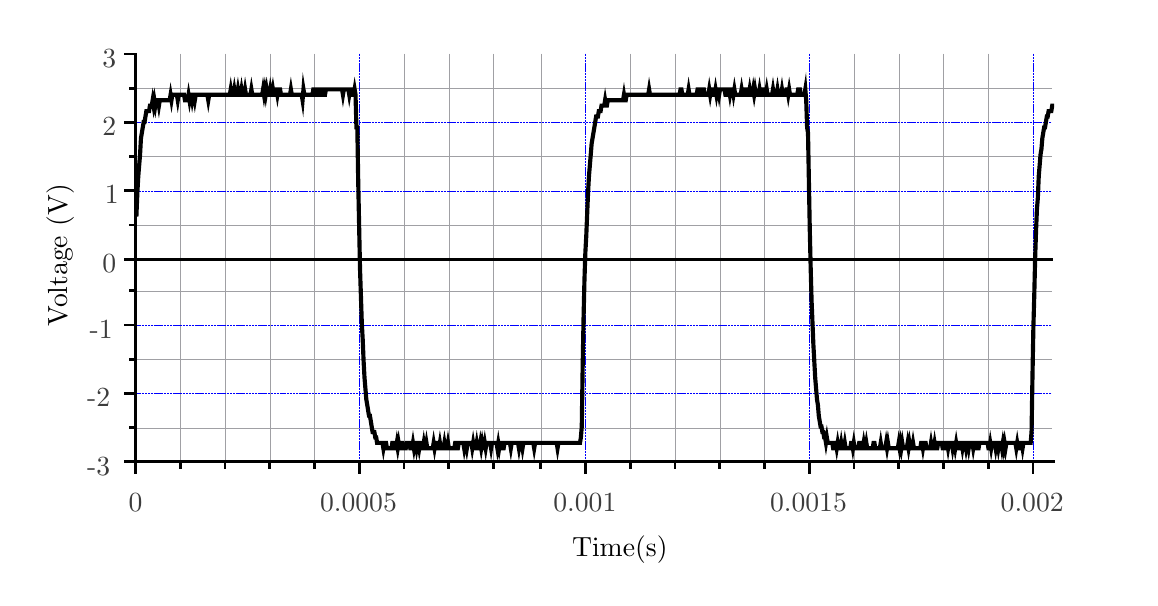
\begin{tikzpicture}{0pt}{0pt}{419pt}{209pt}
	\clip(0pt,209pt) -- (398.436pt,209pt) -- (398.436pt,10.2575pt) -- (0pt,10.2575pt) -- (0pt,209pt);
\begin{scope}
	\clip(38.9878pt,199.491pt) -- (370.859pt,199.491pt) -- (370.859pt,52.098pt) -- (38.9878pt,52.098pt) -- (38.9878pt,199.491pt);
	\color[rgb]{0.627451,0.627451,0.643137}
	\draw[line width=0.1pt, dash pattern=on 0.0024cm off 0.008cm, dash phase=0pt, line join=bevel, line cap=rect](55.1534pt,199.491pt) -- (55.1534pt,53.0489pt);
	\color[rgb]{0.627451,0.627451,0.643137}
	\draw[line width=0.1pt, dash pattern=on 0.0024cm off 0.008cm, dash phase=0pt, line join=bevel, line cap=rect](71.3191pt,199.491pt) -- (71.3191pt,53.0489pt);
	\draw[line width=0.1pt, dash pattern=on 0.0024cm off 0.008cm, dash phase=0pt, line join=bevel, line cap=rect](87.4847pt,199.491pt) -- (87.4847pt,53.0489pt);
	\draw[line width=0.1pt, dash pattern=on 0.0024cm off 0.008cm, dash phase=0pt, line join=bevel, line cap=rect](103.65pt,199.491pt) -- (103.65pt,53.0489pt);
	\draw[line width=0.1pt, dash pattern=on 0.0024cm off 0.008cm, dash phase=0pt, line join=bevel, line cap=rect](135.982pt,199.491pt) -- (135.982pt,53.0489pt);
	\draw[line width=0.1pt, dash pattern=on 0.0024cm off 0.008cm, dash phase=0pt, line join=bevel, line cap=rect](152.147pt,199.491pt) -- (152.147pt,53.0489pt);
	\draw[line width=0.1pt, dash pattern=on 0.0024cm off 0.008cm, dash phase=0pt, line join=bevel, line cap=rect](168.313pt,199.491pt) -- (168.313pt,53.0489pt);
	\draw[line width=0.1pt, dash pattern=on 0.0024cm off 0.008cm, dash phase=0pt, line join=bevel, line cap=rect](185.43pt,199.491pt) -- (185.43pt,53.0489pt);
	\draw[line width=0.1pt, dash pattern=on 0.0024cm off 0.008cm, dash phase=0pt, line join=bevel, line cap=rect](217.761pt,199.491pt) -- (217.761pt,53.0489pt);
	\draw[line width=0.1pt, dash pattern=on 0.0024cm off 0.008cm, dash phase=0pt, line join=bevel, line cap=rect](233.927pt,199.491pt) -- (233.927pt,53.0489pt);
	\draw[line width=0.1pt, dash pattern=on 0.0024cm off 0.008cm, dash phase=0pt, line join=bevel, line cap=rect](250.092pt,199.491pt) -- (250.092pt,53.0489pt);
	\draw[line width=0.1pt, dash pattern=on 0.0024cm off 0.008cm, dash phase=0pt, line join=bevel, line cap=rect](266.258pt,199.491pt) -- (266.258pt,53.0489pt);
	\draw[line width=0.1pt, dash pattern=on 0.0024cm off 0.008cm, dash phase=0pt, line join=bevel, line cap=rect](298.589pt,199.491pt) -- (298.589pt,53.0489pt);
	\draw[line width=0.1pt, dash pattern=on 0.0024cm off 0.008cm, dash phase=0pt, line join=bevel, line cap=rect](314.755pt,199.491pt) -- (314.755pt,53.0489pt);
	\draw[line width=0.1pt, dash pattern=on 0.0024cm off 0.008cm, dash phase=0pt, line join=bevel, line cap=rect](330.921pt,199.491pt) -- (330.921pt,53.0489pt);
	\draw[line width=0.1pt, dash pattern=on 0.0024cm off 0.008cm, dash phase=0pt, line join=bevel, line cap=rect](347.086pt,199.491pt) -- (347.086pt,53.0489pt);
	\draw[line width=0.1pt, dash pattern=on 0.0024cm off 0.008cm, dash phase=0pt, line join=bevel, line cap=rect](38.9878pt,64.46pt) -- (369.908pt,64.46pt);
	\draw[line width=0.1pt, dash pattern=on 0.0024cm off 0.008cm, dash phase=0pt, line join=bevel, line cap=rect](38.9878pt,89.1839pt) -- (369.908pt,89.1839pt);
	\draw[line width=0.1pt, dash pattern=on 0.0024cm off 0.008cm, dash phase=0pt, line join=bevel, line cap=rect](38.9878pt,113.908pt) -- (369.908pt,113.908pt);
	\draw[line width=0.1pt, dash pattern=on 0.0024cm off 0.008cm, dash phase=0pt, line join=bevel, line cap=rect](38.9878pt,137.681pt) -- (369.908pt,137.681pt);
	\draw[line width=0.1pt, dash pattern=on 0.0024cm off 0.008cm, dash phase=0pt, line join=bevel, line cap=rect](38.9878pt,162.405pt) -- (369.908pt,162.405pt);
	\draw[line width=0.1pt, dash pattern=on 0.0024cm off 0.008cm, dash phase=0pt, line join=bevel, line cap=rect](38.9878pt,187.129pt) -- (369.908pt,187.129pt);
	\color[rgb]{0,0,1}
	\draw[line width=0.2pt, dash pattern=on 0.024cm off 0.016cm, dash phase=0pt, line join=bevel, line cap=rect](119.816pt,199.491pt) -- (119.816pt,53.0489pt);
	\draw[line width=0.2pt, dash pattern=on 0.024cm off 0.016cm, dash phase=0pt, line join=bevel, line cap=rect](201.595pt,199.491pt) -- (201.595pt,53.0489pt);
	\draw[line width=0.2pt, dash pattern=on 0.024cm off 0.016cm, dash phase=0pt, line join=bevel, line cap=rect](282.424pt,199.491pt) -- (282.424pt,53.0489pt);
	\draw[line width=0.2pt, dash pattern=on 0.024cm off 0.016cm, dash phase=0pt, line join=bevel, line cap=rect](363.252pt,199.491pt) -- (363.252pt,53.0489pt);
	\draw[line width=0.2pt, dash pattern=on 0.024cm off 0.016cm, dash phase=0pt, line join=bevel, line cap=rect](38.9878pt,76.822pt) -- (369.908pt,76.822pt);
	\draw[line width=0.2pt, dash pattern=on 0.024cm off 0.016cm, dash phase=0pt, line join=bevel, line cap=rect](38.9878pt,101.546pt) -- (369.908pt,101.546pt);
	\draw[line width=0.2pt, dash pattern=on 0.024cm off 0.016cm, dash phase=0pt, line join=bevel, line cap=rect](38.9878pt,125.319pt) -- (369.908pt,125.319pt);
	\draw[line width=0.2pt, dash pattern=on 0.024cm off 0.016cm, dash phase=0pt, line join=bevel, line cap=rect](38.9878pt,150.043pt) -- (369.908pt,150.043pt);
	\draw[line width=0.2pt, dash pattern=on 0.024cm off 0.016cm, dash phase=0pt, line join=bevel, line cap=rect](38.9878pt,174.767pt) -- (369.908pt,174.767pt);
	\color[rgb]{0,0,0}
	\draw[line width=1.5pt, line join=miter, line cap=rect](39.3122pt,141.516pt) -- (39.6366pt,149.377pt) -- (39.961pt,155.273pt) -- (40.2854pt,159.203pt) -- (40.6098pt,163.134pt) -- (40.9342pt,169.03pt) -- (41.2586pt,170.995pt) -- (41.583pt,172.96pt) -- (41.9075pt,174.925pt) -- (42.2319pt,174.925pt) -- (42.5563pt,176.891pt) -- (42.8807pt,178.856pt) -- (43.2051pt,178.856pt) -- (43.5295pt,178.856pt) -- (43.8539pt,178.856pt) -- (44.1783pt,180.821pt) -- (44.5027pt,180.821pt) -- (44.8271pt,180.821pt) -- (45.1516pt,182.786pt) -- (45.476pt,180.821pt) -- (45.8004pt,182.786pt) -- (46.1248pt,180.821pt) -- (46.4492pt,182.786pt) -- (46.7736pt,182.786pt) -- (47.098pt,182.786pt) -- (47.4224pt,180.821pt) -- (47.7468pt,182.786pt) -- (48.0712pt,182.786pt) -- (48.3957pt,182.786pt) -- (48.7201pt,182.786pt) -- (49.0445pt,182.786pt) -- (49.3689pt,182.786pt) -- (49.6933pt,182.786pt) -- (50.0177pt,182.786pt) -- (50.3421pt,182.786pt) -- (50.6665pt,182.786pt) -- (50.9909pt,182.786pt) -- (51.3153pt,182.786pt) -- (51.6398pt,184.752pt) -- (51.9642pt,182.786pt) -- (52.2886pt,184.752pt) -- (52.613pt,184.752pt) -- (52.9374pt,184.752pt) -- (53.2618pt,184.752pt) -- (53.5862pt,184.752pt) -- (53.9106pt,184.752pt) -- (54.235pt,182.786pt) -- (54.5594pt,184.752pt) -- (54.8839pt,184.752pt) -- (55.2083pt,184.752pt) -- (55.5327pt,184.752pt) -- (55.8571pt,184.752pt) -- (56.1815pt,184.752pt) -- (56.5059pt,184.752pt) -- (56.8303pt,182.786pt) -- (57.1547pt,182.786pt) -- (57.4791pt,182.786pt) -- (57.8035pt,182.786pt) -- (58.128pt,184.752pt) -- (58.4524pt,182.786pt) -- (58.7768pt,184.752pt) -- (59.1012pt,184.752pt) -- (59.4256pt,182.786pt) -- (59.75pt,184.752pt) -- (60.0744pt,184.752pt) -- (60.3988pt,182.786pt) -- (60.7232pt,184.752pt) -- (61.0476pt,184.752pt) -- (61.3721pt,184.752pt) -- (61.6965pt,184.752pt) -- (62.0209pt,184.752pt) -- (62.3453pt,184.752pt) -- (62.6697pt,184.752pt) -- (62.9941pt,184.752pt) -- (63.3185pt,184.752pt) -- (63.6429pt,184.752pt) -- (63.9673pt,184.752pt) -- (64.2917pt,184.752pt) -- (64.6162pt,184.752pt) -- (64.9406pt,184.752pt) -- (65.265pt,182.786pt) -- (65.5894pt,184.752pt) -- (65.9138pt,184.752pt) -- (66.2382pt,184.752pt) -- (66.5626pt,184.752pt) -- (66.887pt,184.752pt) -- (67.2114pt,184.752pt) -- (67.5358pt,184.752pt) -- (67.8603pt,184.752pt) -- (68.1847pt,184.752pt) -- (68.5091pt,184.752pt) -- (68.8335pt,184.752pt) -- (69.1579pt,184.752pt) -- (69.4823pt,184.752pt) -- (69.8067pt,184.752pt) -- (70.1311pt,184.752pt) -- (70.4555pt,184.752pt) -- (70.7799pt,184.752pt) -- (71.1044pt,184.752pt) -- (71.4288pt,184.752pt) -- (71.7532pt,184.752pt) -- (72.0776pt,184.752pt) -- (72.402pt,184.752pt) -- (72.7264pt,184.752pt) -- (73.0508pt,184.752pt) -- (73.3752pt,186.717pt) -- (73.6996pt,184.752pt) -- (74.024pt,184.752pt) -- (74.3485pt,184.752pt) -- (74.6729pt,186.717pt) -- (74.9973pt,184.752pt) -- (75.3217pt,184.752pt) -- (75.6461pt,184.752pt) -- (75.9705pt,186.717pt) -- (76.2949pt,184.752pt) -- (76.6193pt,184.752pt) -- (76.9437pt,184.752pt) -- (77.2681pt,186.717pt) -- (77.5926pt,184.752pt) -- (77.917pt,184.752pt) -- (78.2414pt,184.752pt) -- (78.5658pt,186.717pt) -- (78.8902pt,184.752pt) -- (79.2146pt,184.752pt) -- (79.539pt,184.752pt) -- (79.8634pt,184.752pt) -- (80.1878pt,184.752pt) -- (80.5122pt,184.752pt) -- (80.8367pt,186.717pt) -- (81.1611pt,184.752pt) -- (81.4855pt,184.752pt) -- (81.8099pt,184.752pt) -- (82.1343pt,184.752pt) -- (82.4587pt,184.752pt) -- (82.7831pt,184.752pt) -- (83.1075pt,184.752pt) -- (83.4319pt,184.752pt) -- (83.7563pt,184.752pt) -- (84.0808pt,184.752pt) -- (84.4052pt,184.752pt) -- (84.7296pt,184.752pt) -- (85.054pt,186.717pt) -- (85.3784pt,184.752pt) -- (85.7028pt,186.717pt) -- (86.0272pt,184.752pt) -- (86.3516pt,186.717pt) -- (86.676pt,184.752pt) -- (87.0004pt,184.752pt) -- (87.3249pt,184.752pt) -- (87.6493pt,186.717pt) -- (87.9737pt,184.752pt) -- (88.2981pt,184.752pt) -- (88.6225pt,186.717pt) -- (88.9469pt,184.752pt) -- (89.2713pt,184.752pt) -- (89.5957pt,186.717pt) -- (89.9201pt,186.717pt) -- (90.2445pt,184.752pt) -- (90.569pt,186.717pt) -- (90.8934pt,186.717pt) -- (91.2178pt,186.717pt) -- (91.5422pt,184.752pt) -- (91.8666pt,184.752pt) -- (92.191pt,184.752pt) -- (92.5154pt,184.752pt) -- (92.8398pt,184.752pt) -- (93.1642pt,184.752pt) -- (93.4886pt,184.752pt) -- (93.8131pt,184.752pt) -- (94.1375pt,184.752pt) -- (94.4619pt,184.752pt) -- (94.7863pt,184.752pt) -- (95.1107pt,186.717pt) -- (95.4351pt,184.752pt) -- (95.7595pt,184.752pt) -- (96.0839pt,184.752pt) -- (96.4083pt,184.752pt) -- (96.7327pt,184.752pt) -- (97.0572pt,184.752pt) -- (97.3816pt,184.752pt) -- (97.706pt,184.752pt) -- (98.0304pt,184.752pt) -- (98.3548pt,184.752pt) -- (98.6792pt,184.752pt) -- (99.0036pt,184.752pt) -- (99.328pt,182.786pt) -- (99.6524pt,186.717pt) -- (99.9768pt,184.752pt) -- (100.301pt,184.752pt) -- (100.626pt,184.752pt) -- (100.95pt,184.752pt) -- (101.274pt,184.752pt) -- (101.599pt,184.752pt) -- (101.923pt,184.752pt) -- (102.248pt,184.752pt) -- (102.572pt,184.752pt) -- (102.897pt,184.752pt) -- (103.221pt,186.717pt) -- (103.545pt,186.717pt) -- (103.87pt,184.752pt) -- (104.194pt,184.752pt) -- (104.519pt,184.752pt) -- (104.843pt,186.717pt) -- (105.167pt,186.717pt) -- (105.492pt,184.752pt) -- (105.816pt,184.752pt) -- (106.141pt,186.717pt) -- (106.465pt,186.717pt) -- (106.789pt,186.717pt) -- (107.114pt,184.752pt) -- (107.438pt,184.752pt) -- (107.763pt,186.717pt) -- (108.087pt,186.717pt) -- (108.412pt,186.717pt) -- (108.736pt,186.717pt) -- (109.06pt,186.717pt) -- (109.385pt,186.717pt) -- (109.709pt,186.717pt) -- (110.034pt,186.717pt) -- (110.358pt,186.717pt) -- (110.682pt,186.717pt) -- (111.007pt,186.717pt) -- (111.331pt,186.717pt) -- (111.656pt,186.717pt) -- (111.98pt,186.717pt) -- (112.304pt,186.717pt) -- (112.629pt,186.717pt) -- (112.953pt,186.717pt) -- (113.278pt,186.717pt) -- (113.602pt,186.717pt) -- (113.926pt,184.752pt) -- (114.251pt,186.717pt) -- (114.575pt,186.717pt) -- (114.9pt,186.717pt) -- (115.224pt,186.717pt) -- (115.549pt,186.717pt) -- (115.873pt,186.717pt) -- (116.197pt,184.752pt) -- (116.522pt,186.717pt) -- (116.846pt,186.717pt) -- (117.171pt,186.717pt) -- (117.495pt,184.752pt) -- (117.819pt,184.752pt) -- (118.144pt,186.717pt) -- (118.468pt,184.752pt) -- (118.793pt,172.96pt) -- (119.117pt,172.96pt) -- (119.441pt,153.308pt) -- (119.766pt,137.586pt) -- (120.09pt,121.864pt) -- (120.415pt,112.038pt) -- (120.739pt,102.212pt) -- (121.063pt,96.3159pt) -- (121.388pt,88.4549pt) -- (121.712pt,82.5592pt) -- (122.037pt,78.6287pt) -- (122.361pt,74.6982pt) -- (122.686pt,72.733pt) -- (123.01pt,70.7678pt) -- (123.334pt,68.8025pt) -- (123.659pt,68.8025pt) -- (123.983pt,66.8373pt) -- (124.308pt,64.8721pt) -- (124.632pt,62.9068pt) -- (124.956pt,62.9068pt) -- (125.281pt,62.9068pt) -- (125.605pt,60.9416pt) -- (125.93pt,60.9416pt) -- (126.254pt,58.9764pt) -- (126.578pt,58.9764pt) -- (126.903pt,58.9764pt) -- (127.227pt,58.9764pt) -- (127.552pt,58.9764pt) -- (127.876pt,58.9764pt) -- (128.201pt,58.9764pt) -- (128.525pt,57.0111pt) -- (128.849pt,58.9764pt) -- (129.174pt,58.9764pt) -- (129.498pt,58.9764pt) -- (129.823pt,57.0111pt) -- (130.147pt,57.0111pt) -- (130.471pt,57.0111pt) -- (130.796pt,57.0111pt) -- (131.12pt,57.0111pt) -- (131.445pt,57.0111pt) -- (131.769pt,58.9764pt) -- (132.093pt,58.9764pt) -- (132.418pt,57.0111pt) -- (132.742pt,57.0111pt) -- (133.067pt,57.0111pt) -- (133.391pt,58.9764pt) -- (133.715pt,57.0111pt) -- (134.04pt,58.9764pt) -- (134.364pt,57.0111pt) -- (134.689pt,57.0111pt) -- (135.013pt,58.9764pt) -- (135.338pt,58.9764pt) -- (135.662pt,57.0111pt) -- (135.986pt,57.0111pt) -- (136.311pt,57.0111pt) -- (136.635pt,57.0111pt) -- (136.96pt,58.9764pt) -- (137.284pt,58.9764pt) -- (137.608pt,58.9764pt) -- (137.933pt,58.9764pt) -- (138.257pt,57.0111pt) -- (138.582pt,57.0111pt) -- (138.906pt,57.0111pt) -- (139.23pt,58.9764pt) -- (139.555pt,57.0111pt) -- (139.879pt,58.9764pt) -- (140.204pt,58.9764pt) -- (140.528pt,57.0111pt) -- (140.853pt,58.9764pt) -- (141.177pt,58.9764pt) -- (141.501pt,57.0111pt) -- (141.826pt,58.9764pt) -- (142.15pt,58.9764pt) -- (142.475pt,57.0111pt) -- (142.799pt,57.0111pt) -- (143.123pt,58.9764pt) -- (143.448pt,57.0111pt) -- (143.772pt,57.0111pt) -- (144.097pt,58.9764pt) -- (144.421pt,57.0111pt) -- (144.745pt,57.0111pt) -- (145.07pt,57.0111pt) -- (145.394pt,57.0111pt) -- (145.719pt,57.0111pt) -- (146.043pt,57.0111pt) -- (146.367pt,57.0111pt) -- (146.692pt,58.9764pt) -- (147.016pt,57.0111pt) -- (147.341pt,58.9764pt) -- (147.665pt,58.9764pt) -- (147.99pt,57.0111pt) -- (148.314pt,57.0111pt) -- (148.638pt,57.0111pt) -- (148.963pt,58.9764pt) -- (149.287pt,57.0111pt) -- (149.612pt,57.0111pt) -- (149.936pt,57.0111pt) -- (150.26pt,57.0111pt) -- (150.585pt,58.9764pt) -- (150.909pt,57.0111pt) -- (151.234pt,57.0111pt) -- (151.558pt,57.0111pt) -- (151.882pt,58.9764pt) -- (152.207pt,57.0111pt) -- (152.531pt,57.0111pt) -- (152.856pt,57.0111pt) -- (153.18pt,57.0111pt) -- (153.504pt,57.0111pt) -- (153.829pt,57.0111pt) -- (154.153pt,57.0111pt) -- (154.478pt,58.9764pt) -- (154.802pt,58.9764pt) -- (155.127pt,57.0111pt) -- (155.451pt,57.0111pt) -- (155.775pt,58.9764pt) -- (156.1pt,58.9764pt) -- (156.424pt,58.9764pt) -- (156.749pt,58.9764pt) -- (157.073pt,58.9764pt) -- (157.397pt,58.9764pt) -- (157.722pt,57.0111pt) -- (158.046pt,58.9764pt) -- (158.371pt,58.9764pt) -- (158.695pt,57.0111pt) -- (159.019pt,58.9764pt) -- (159.344pt,58.9764pt) -- (159.668pt,58.9764pt) -- (159.993pt,58.9764pt) -- (160.317pt,58.9764pt) -- (160.642pt,57.0111pt) -- (160.966pt,58.9764pt) -- (161.29pt,57.0111pt) -- (161.615pt,57.0111pt) -- (161.939pt,57.0111pt) -- (162.264pt,58.9764pt) -- (162.588pt,57.0111pt) -- (162.912pt,57.0111pt) -- (163.237pt,57.0111pt) -- (163.561pt,58.9764pt) -- (163.886pt,57.0111pt) -- (164.21pt,58.9764pt) -- (164.534pt,57.0111pt) -- (164.859pt,57.0111pt) -- (165.183pt,58.9764pt) -- (165.508pt,57.0111pt) -- (165.832pt,58.9764pt) -- (166.156pt,58.9764pt) -- (166.481pt,58.9764pt) -- (166.805pt,58.9764pt) -- (167.13pt,58.9764pt) -- (167.454pt,57.0111pt) -- (167.779pt,58.9764pt) -- (168.103pt,58.9764pt) -- (168.427pt,58.9764pt) -- (168.752pt,58.9764pt) -- (169.076pt,58.9764pt) -- (169.401pt,58.9764pt) -- (169.725pt,57.0111pt) -- (170.049pt,58.9764pt) -- (170.374pt,57.0111pt) -- (170.698pt,58.9764pt) -- (171.023pt,58.9764pt) -- (171.347pt,58.9764pt) -- (171.671pt,57.0111pt) -- (171.996pt,57.0111pt) -- (172.32pt,58.9764pt) -- (172.645pt,58.9764pt) -- (172.969pt,58.9764pt) -- (173.294pt,58.9764pt) -- (173.618pt,58.9764pt) -- (173.942pt,58.9764pt) -- (174.267pt,58.9764pt) -- (174.591pt,57.0111pt) -- (174.916pt,58.9764pt) -- (175.24pt,58.9764pt) -- (175.564pt,58.9764pt) -- (175.889pt,58.9764pt) -- (176.213pt,58.9764pt) -- (176.538pt,58.9764pt) -- (176.862pt,58.9764pt) -- (177.186pt,58.9764pt) -- (177.511pt,57.0111pt) -- (177.835pt,58.9764pt) -- (178.16pt,58.9764pt) -- (178.484pt,58.9764pt) -- (178.808pt,57.0111pt) -- (179.133pt,58.9764pt) -- (179.457pt,58.9764pt) -- (179.782pt,58.9764pt) -- (180.106pt,58.9764pt) -- (180.431pt,58.9764pt) -- (180.755pt,58.9764pt) -- (181.079pt,58.9764pt) -- (181.404pt,58.9764pt) -- (181.728pt,58.9764pt) -- (182.053pt,58.9764pt) -- (182.377pt,58.9764pt) -- (182.701pt,58.9764pt) -- (183.026pt,57.0111pt) -- (183.35pt,58.9764pt) -- (183.675pt,58.9764pt) -- (183.999pt,58.9764pt) -- (184.323pt,58.9764pt) -- (184.648pt,58.9764pt) -- (184.972pt,58.9764pt) -- (185.297pt,58.9764pt) -- (185.621pt,58.9764pt) -- (185.946pt,58.9764pt) -- (186.27pt,58.9764pt) -- (186.594pt,58.9764pt) -- (186.919pt,58.9764pt) -- (187.243pt,58.9764pt) -- (187.568pt,58.9764pt) -- (187.892pt,58.9764pt) -- (188.216pt,58.9764pt) -- (188.541pt,58.9764pt) -- (188.865pt,58.9764pt) -- (189.19pt,58.9764pt) -- (189.514pt,58.9764pt) -- (189.838pt,58.9764pt) -- (190.163pt,58.9764pt) -- (190.487pt,58.9764pt) -- (190.812pt,58.9764pt) -- (191.136pt,58.9764pt) -- (191.46pt,57.0111pt) -- (191.785pt,58.9764pt) -- (192.109pt,58.9764pt) -- (192.434pt,58.9764pt) -- (192.758pt,58.9764pt) -- (193.083pt,58.9764pt) -- (193.407pt,58.9764pt) -- (193.731pt,58.9764pt) -- (194.056pt,58.9764pt) -- (194.38pt,58.9764pt) -- (194.705pt,58.9764pt) -- (195.029pt,58.9764pt) -- (195.353pt,58.9764pt) -- (195.678pt,58.9764pt) -- (196.002pt,58.9764pt) -- (196.327pt,58.9764pt) -- (196.651pt,58.9764pt) -- (196.975pt,58.9764pt) -- (197.3pt,58.9764pt) -- (197.624pt,58.9764pt) -- (197.949pt,58.9764pt) -- (198.273pt,58.9764pt) -- (198.597pt,58.9764pt) -- (198.922pt,58.9764pt) -- (199.246pt,58.9764pt) -- (199.571pt,58.9764pt) -- (199.895pt,60.9416pt) -- (200.22pt,64.8721pt) -- (200.544pt,86.4897pt) -- (200.868pt,104.177pt) -- (201.193pt,117.933pt) -- (201.517pt,127.76pt) -- (201.842pt,133.655pt) -- (202.166pt,141.516pt) -- (202.49pt,149.377pt) -- (202.815pt,155.273pt) -- (203.139pt,159.203pt) -- (203.464pt,163.134pt) -- (203.788pt,167.064pt) -- (204.112pt,169.03pt) -- (204.437pt,170.995pt) -- (204.761pt,172.96pt) -- (205.086pt,174.925pt) -- (205.41pt,176.891pt) -- (205.735pt,176.891pt) -- (206.059pt,176.891pt) -- (206.383pt,178.856pt) -- (206.708pt,178.856pt) -- (207.032pt,178.856pt) -- (207.357pt,180.821pt) -- (207.681pt,180.821pt) -- (208.005pt,180.821pt) -- (208.33pt,180.821pt) -- (208.654pt,182.786pt) -- (208.979pt,180.821pt) -- (209.303pt,180.821pt) -- (209.627pt,182.786pt) -- (209.952pt,182.786pt) -- (210.276pt,182.786pt) -- (210.601pt,182.786pt) -- (210.925pt,182.786pt) -- (211.249pt,182.786pt) -- (211.574pt,182.786pt) -- (211.898pt,182.786pt) -- (212.223pt,182.786pt) -- (212.547pt,182.786pt) -- (212.872pt,182.786pt) -- (213.196pt,182.786pt) -- (213.52pt,182.786pt) -- (213.845pt,182.786pt) -- (214.169pt,182.786pt) -- (214.494pt,182.786pt) -- (214.818pt,182.786pt) -- (215.142pt,182.786pt) -- (215.467pt,184.752pt) -- (215.791pt,182.786pt) -- (216.116pt,182.786pt) -- (216.44pt,184.752pt) -- (216.764pt,184.752pt) -- (217.089pt,184.752pt) -- (217.413pt,184.752pt) -- (217.738pt,184.752pt) -- (218.062pt,184.752pt) -- (218.387pt,184.752pt) -- (218.711pt,184.752pt) -- (219.035pt,184.752pt) -- (219.36pt,184.752pt) -- (219.684pt,184.752pt) -- (220.009pt,184.752pt) -- (220.333pt,184.752pt) -- (220.657pt,184.752pt) -- (220.982pt,184.752pt) -- (221.306pt,184.752pt) -- (221.631pt,184.752pt) -- (221.955pt,184.752pt) -- (222.279pt,184.752pt) -- (222.604pt,184.752pt) -- (222.928pt,184.752pt) -- (223.253pt,184.752pt) -- (223.577pt,184.752pt) -- (223.901pt,184.752pt) -- (224.226pt,184.752pt) -- (224.55pt,186.717pt) -- (224.875pt,184.752pt) -- (225.199pt,184.752pt) -- (225.524pt,184.752pt) -- (225.848pt,184.752pt) -- (226.172pt,184.752pt) -- (226.497pt,184.752pt) -- (226.821pt,184.752pt) -- (227.146pt,184.752pt) -- (227.47pt,184.752pt) -- (227.794pt,184.752pt) -- (228.119pt,184.752pt) -- (228.443pt,184.752pt) -- (228.768pt,184.752pt) -- (229.092pt,184.752pt) -- (229.416pt,184.752pt) -- (229.741pt,184.752pt) -- (230.065pt,184.752pt) -- (230.39pt,184.752pt) -- (230.714pt,184.752pt) -- (231.038pt,184.752pt) -- (231.363pt,184.752pt) -- (231.687pt,184.752pt) -- (232.012pt,184.752pt) -- (232.336pt,184.752pt) -- (232.661pt,184.752pt) -- (232.985pt,184.752pt) -- (233.309pt,184.752pt) -- (233.634pt,184.752pt) -- (233.958pt,184.752pt) -- (234.283pt,184.752pt) -- (234.607pt,184.752pt) -- (234.931pt,184.752pt) -- (235.256pt,184.752pt) -- (235.58pt,184.752pt) -- (235.905pt,186.717pt) -- (236.229pt,186.717pt) -- (236.553pt,184.752pt) -- (236.878pt,184.752pt) -- (237.202pt,184.752pt) -- (237.527pt,184.752pt) -- (237.851pt,184.752pt) -- (238.176pt,184.752pt) -- (238.5pt,184.752pt) -- (238.824pt,186.717pt) -- (239.149pt,184.752pt) -- (239.473pt,184.752pt) -- (239.798pt,184.752pt) -- (240.122pt,184.752pt) -- (240.446pt,184.752pt) -- (240.771pt,184.752pt) -- (241.095pt,184.752pt) -- (241.42pt,184.752pt) -- (241.744pt,184.752pt) -- (242.068pt,186.717pt) -- (242.393pt,186.717pt) -- (242.717pt,184.752pt) -- (243.042pt,184.752pt) -- (243.366pt,184.752pt) -- (243.69pt,186.717pt) -- (244.015pt,186.717pt) -- (244.339pt,186.717pt) -- (244.664pt,184.752pt) -- (244.988pt,184.752pt) -- (245.313pt,184.752pt) -- (245.637pt,184.752pt) -- (245.961pt,184.752pt) -- (246.286pt,186.717pt) -- (246.61pt,184.752pt) -- (246.935pt,186.717pt) -- (247.259pt,186.717pt) -- (247.583pt,186.717pt) -- (247.908pt,184.752pt) -- (248.232pt,184.752pt) -- (248.557pt,186.717pt) -- (248.881pt,184.752pt) -- (249.205pt,186.717pt) -- (249.53pt,186.717pt) -- (249.854pt,184.752pt) -- (250.179pt,186.717pt) -- (250.503pt,186.717pt) -- (250.828pt,186.717pt) -- (251.152pt,186.717pt) -- (251.476pt,186.717pt) -- (251.801pt,186.717pt) -- (252.125pt,184.752pt) -- (252.45pt,184.752pt) -- (252.774pt,186.717pt) -- (253.098pt,186.717pt) -- (253.423pt,186.717pt) -- (253.747pt,184.752pt) -- (254.072pt,186.717pt) -- (254.396pt,186.717pt) -- (254.72pt,186.717pt) -- (255.045pt,184.752pt) -- (255.369pt,186.717pt) -- (255.694pt,184.752pt) -- (256.018pt,184.752pt) -- (256.342pt,184.752pt) -- (256.667pt,184.752pt) -- (256.991pt,184.752pt) -- (257.316pt,184.752pt) -- (257.64pt,184.752pt) -- (257.965pt,186.717pt) -- (258.289pt,184.752pt) -- (258.613pt,184.752pt) -- (258.938pt,186.717pt) -- (259.262pt,186.717pt) -- (259.587pt,186.717pt) -- (259.911pt,184.752pt) -- (260.235pt,184.752pt) -- (260.56pt,184.752pt) -- (260.884pt,186.717pt) -- (261.209pt,184.752pt) -- (261.533pt,184.752pt) -- (261.857pt,184.752pt) -- (262.182pt,186.717pt) -- (262.506pt,184.752pt) -- (262.831pt,186.717pt) -- (263.155pt,184.752pt) -- (263.479pt,184.752pt) -- (263.804pt,184.752pt) -- (264.128pt,184.752pt) -- (264.453pt,186.717pt) -- (264.777pt,184.752pt) -- (265.102pt,184.752pt) -- (265.426pt,186.717pt) -- (265.75pt,186.717pt) -- (266.075pt,184.752pt) -- (266.399pt,184.752pt) -- (266.724pt,184.752pt) -- (267.048pt,186.717pt) -- (267.372pt,184.752pt) -- (267.697pt,184.752pt) -- (268.021pt,184.752pt) -- (268.346pt,184.752pt) -- (268.67pt,184.752pt) -- (268.994pt,184.752pt) -- (269.319pt,186.717pt) -- (269.643pt,184.752pt) -- (269.968pt,184.752pt) -- (270.292pt,184.752pt) -- (270.617pt,184.752pt) -- (270.941pt,186.717pt) -- (271.265pt,184.752pt) -- (271.59pt,184.752pt) -- (271.914pt,184.752pt) -- (272.239pt,184.752pt) -- (272.563pt,186.717pt) -- (272.887pt,184.752pt) -- (273.212pt,184.752pt) -- (273.536pt,184.752pt) -- (273.861pt,184.752pt) -- (274.185pt,186.717pt) -- (274.509pt,186.717pt) -- (274.834pt,184.752pt) -- (275.158pt,186.717pt) -- (275.483pt,184.752pt) -- (275.807pt,184.752pt) -- (276.131pt,184.752pt) -- (276.456pt,184.752pt) -- (276.78pt,184.752pt) -- (277.105pt,184.752pt) -- (277.429pt,184.752pt) -- (277.754pt,184.752pt) -- (278.078pt,184.752pt) -- (278.402pt,186.717pt) -- (278.727pt,186.717pt) -- (279.051pt,186.717pt) -- (279.376pt,184.752pt) -- (279.7pt,184.752pt) -- (280.024pt,184.752pt) -- (280.349pt,184.752pt) -- (280.673pt,184.752pt) -- (280.998pt,186.717pt) -- (281.322pt,182.786pt) -- (281.646pt,172.96pt) -- (281.971pt,170.995pt) -- (282.295pt,153.308pt) -- (282.62pt,135.621pt) -- (282.944pt,121.864pt) -- (283.269pt,110.073pt) -- (283.593pt,102.212pt) -- (283.917pt,94.3506pt) -- (284.242pt,88.4549pt) -- (284.566pt,82.5592pt) -- (284.891pt,78.6287pt) -- (285.215pt,74.6982pt) -- (285.539pt,72.733pt) -- (285.864pt,68.8025pt) -- (286.188pt,66.8373pt) -- (286.513pt,64.8721pt) -- (286.837pt,64.8721pt) -- (287.161pt,62.9068pt) -- (287.486pt,62.9068pt) -- (287.81pt,60.9416pt) -- (288.135pt,60.9416pt) -- (288.459pt,58.9764pt) -- (288.783pt,60.9416pt) -- (289.108pt,58.9764pt) -- (289.432pt,58.9764pt) -- (289.757pt,58.9764pt) -- (290.081pt,58.9764pt) -- (290.406pt,58.9764pt) -- (290.73pt,58.9764pt) -- (291.054pt,57.0111pt) -- (291.379pt,57.0111pt) -- (291.703pt,58.9764pt) -- (292.028pt,58.9764pt) -- (292.352pt,57.0111pt) -- (292.676pt,58.9764pt) -- (293.001pt,57.0111pt) -- (293.325pt,57.0111pt) -- (293.65pt,57.0111pt) -- (293.974pt,58.9764pt) -- (294.298pt,57.0111pt) -- (294.623pt,57.0111pt) -- (294.947pt,57.0111pt) -- (295.272pt,58.9764pt) -- (295.596pt,57.0111pt) -- (295.92pt,57.0111pt) -- (296.245pt,57.0111pt) -- (296.569pt,57.0111pt) -- (296.894pt,57.0111pt) -- (297.218pt,57.0111pt) -- (297.543pt,58.9764pt) -- (297.867pt,58.9764pt) -- (298.191pt,57.0111pt) -- (298.516pt,58.9764pt) -- (298.84pt,57.0111pt) -- (299.165pt,57.0111pt) -- (299.489pt,57.0111pt) -- (299.813pt,57.0111pt) -- (300.138pt,57.0111pt) -- (300.462pt,58.9764pt) -- (300.787pt,58.9764pt) -- (301.111pt,57.0111pt) -- (301.435pt,57.0111pt) -- (301.76pt,57.0111pt) -- (302.084pt,58.9764pt) -- (302.409pt,57.0111pt) -- (302.733pt,57.0111pt) -- (303.058pt,58.9764pt) -- (303.382pt,57.0111pt) -- (303.706pt,57.0111pt) -- (304.031pt,57.0111pt) -- (304.355pt,57.0111pt) -- (304.68pt,57.0111pt) -- (305.004pt,57.0111pt) -- (305.328pt,57.0111pt) -- (305.653pt,58.9764pt) -- (305.977pt,58.9764pt) -- (306.302pt,57.0111pt) -- (306.626pt,57.0111pt) -- (306.95pt,57.0111pt) -- (307.275pt,57.0111pt) -- (307.599pt,57.0111pt) -- (307.924pt,57.0111pt) -- (308.248pt,58.9764pt) -- (308.572pt,57.0111pt) -- (308.897pt,57.0111pt) -- (309.221pt,57.0111pt) -- (309.546pt,57.0111pt) -- (309.87pt,57.0111pt) -- (310.195pt,58.9764pt) -- (310.519pt,57.0111pt) -- (310.843pt,58.9764pt) -- (311.168pt,57.0111pt) -- (311.492pt,57.0111pt) -- (311.817pt,57.0111pt) -- (312.141pt,57.0111pt) -- (312.465pt,57.0111pt) -- (312.79pt,57.0111pt) -- (313.114pt,57.0111pt) -- (313.439pt,57.0111pt) -- (313.763pt,57.0111pt) -- (314.087pt,57.0111pt) -- (314.412pt,57.0111pt) -- (314.736pt,58.9764pt) -- (315.061pt,57.0111pt) -- (315.385pt,58.9764pt) -- (315.71pt,57.0111pt) -- (316.034pt,58.9764pt) -- (316.358pt,57.0111pt) -- (316.683pt,57.0111pt) -- (317.007pt,57.0111pt) -- (317.332pt,57.0111pt) -- (317.656pt,57.0111pt) -- (317.98pt,58.9764pt) -- (318.305pt,57.0111pt) -- (318.629pt,58.9764pt) -- (318.954pt,57.0111pt) -- (319.278pt,57.0111pt) -- (319.602pt,57.0111pt) -- (319.927pt,58.9764pt) -- (320.251pt,57.0111pt) -- (320.576pt,57.0111pt) -- (320.9pt,57.0111pt) -- (321.224pt,57.0111pt) -- (321.549pt,57.0111pt) -- (321.873pt,57.0111pt) -- (322.198pt,57.0111pt) -- (322.522pt,57.0111pt) -- (322.847pt,58.9764pt) -- (323.171pt,58.9764pt) -- (323.495pt,57.0111pt) -- (323.82pt,58.9764pt) -- (324.144pt,58.9764pt) -- (324.469pt,58.9764pt) -- (324.793pt,57.0111pt) -- (325.117pt,57.0111pt) -- (325.442pt,57.0111pt) -- (325.766pt,57.0111pt) -- (326.091pt,57.0111pt) -- (326.415pt,58.9764pt) -- (326.739pt,57.0111pt) -- (327.064pt,57.0111pt) -- (327.388pt,57.0111pt) -- (327.713pt,58.9764pt) -- (328.037pt,57.0111pt) -- (328.361pt,57.0111pt) -- (328.686pt,57.0111pt) -- (329.01pt,58.9764pt) -- (329.335pt,58.9764pt) -- (329.659pt,58.9764pt) -- (329.984pt,58.9764pt) -- (330.308pt,58.9764pt) -- (330.632pt,57.0111pt) -- (330.957pt,57.0111pt) -- (331.281pt,57.0111pt) -- (331.606pt,58.9764pt) -- (331.93pt,58.9764pt) -- (332.254pt,58.9764pt) -- (332.579pt,57.0111pt) -- (332.903pt,58.9764pt) -- (333.228pt,58.9764pt) -- (333.552pt,58.9764pt) -- (333.876pt,58.9764pt) -- (334.201pt,57.0111pt) -- (334.525pt,58.9764pt) -- (334.85pt,58.9764pt) -- (335.174pt,57.0111pt) -- (335.499pt,58.9764pt) -- (335.823pt,57.0111pt) -- (336.147pt,57.0111pt) -- (336.472pt,57.0111pt) -- (336.796pt,58.9764pt) -- (337.121pt,58.9764pt) -- (337.445pt,58.9764pt) -- (337.769pt,57.0111pt) -- (338.094pt,58.9764pt) -- (338.418pt,58.9764pt) -- (338.743pt,58.9764pt) -- (339.067pt,57.0111pt) -- (339.391pt,58.9764pt) -- (339.716pt,58.9764pt) -- (340.04pt,57.0111pt) -- (340.365pt,58.9764pt) -- (340.689pt,58.9764pt) -- (341.013pt,58.9764pt) -- (341.338pt,58.9764pt) -- (341.662pt,57.0111pt) -- (341.987pt,58.9764pt) -- (342.311pt,58.9764pt) -- (342.636pt,58.9764pt) -- (342.96pt,57.0111pt) -- (343.284pt,57.0111pt) -- (343.609pt,57.0111pt) -- (343.933pt,58.9764pt) -- (344.258pt,58.9764pt) -- (344.582pt,58.9764pt) -- (344.906pt,58.9764pt) -- (345.231pt,58.9764pt) -- (345.555pt,58.9764pt) -- (345.88pt,58.9764pt) -- (346.204pt,58.9764pt) -- (346.528pt,58.9764pt) -- (346.853pt,58.9764pt) -- (347.177pt,57.0111pt) -- (347.502pt,57.0111pt) -- (347.826pt,58.9764pt) -- (348.151pt,57.0111pt) -- (348.475pt,58.9764pt) -- (348.799pt,58.9764pt) -- (349.124pt,58.9764pt) -- (349.448pt,58.9764pt) -- (349.773pt,57.0111pt) -- (350.097pt,58.9764pt) -- (350.421pt,58.9764pt) -- (350.746pt,57.0111pt) -- (351.07pt,58.9764pt) -- (351.395pt,58.9764pt) -- (351.719pt,58.9764pt) -- (352.043pt,57.0111pt) -- (352.368pt,58.9764pt) -- (352.692pt,57.0111pt) -- (353.017pt,58.9764pt) -- (353.341pt,57.0111pt) -- (353.665pt,58.9764pt) -- (353.99pt,58.9764pt) -- (354.314pt,58.9764pt) -- (354.639pt,58.9764pt) -- (354.963pt,58.9764pt) -- (355.288pt,58.9764pt) -- (355.612pt,58.9764pt) -- (355.936pt,58.9764pt) -- (356.261pt,58.9764pt) -- (356.585pt,58.9764pt) -- (356.91pt,58.9764pt) -- (357.234pt,57.0111pt) -- (357.558pt,58.9764pt) -- (357.883pt,57.0111pt) -- (358.207pt,57.0111pt) -- (358.532pt,57.0111pt) -- (358.856pt,58.9764pt) -- (359.18pt,58.9764pt) -- (359.505pt,57.0111pt) -- (359.829pt,58.9764pt) -- (360.154pt,58.9764pt) -- (360.478pt,58.9764pt) -- (360.803pt,58.9764pt) -- (361.127pt,58.9764pt) -- (361.451pt,58.9764pt) -- (361.776pt,58.9764pt) -- (362.1pt,58.9764pt) -- (362.425pt,58.9764pt) -- (362.749pt,62.9068pt) -- (363.073pt,82.5592pt) -- (363.398pt,100.246pt) -- (363.722pt,112.038pt) -- (364.047pt,125.794pt) -- (364.371pt,135.621pt) -- (364.695pt,143.482pt) -- (365.02pt,147.412pt) -- (365.344pt,155.273pt) -- (365.669pt,159.203pt) -- (365.993pt,163.134pt) -- (366.317pt,165.099pt) -- (366.642pt,169.03pt) -- (366.966pt,170.995pt) -- (367.291pt,172.96pt) -- (367.615pt,172.96pt) -- (367.94pt,174.925pt) -- (368.264pt,176.891pt) -- (368.588pt,176.891pt) -- (368.913pt,178.856pt) -- (369.237pt,178.856pt) -- (369.562pt,178.856pt) -- (369.886pt,178.856pt) -- (370.21pt,180.821pt) -- (370.535pt,180.821pt) -- (370.859pt,180.821pt);
	\draw[line width=1pt, line join=bevel, line cap=rect](38.9878pt,125.319pt) -- (369.908pt,125.319pt);
\end{scope}
\begin{scope}
	\color[rgb]{0,0,0}
	\pgftext[center, base, at={\pgfpoint{14.2638pt}{126.738pt}},rotate=90]{Voltage (V)}
	\color[rgb]{0.235294,0.235294,0.235294}
	\pgftext[center, base, at={\pgfpoint{25.6154pt}{47.3434pt}}]{-3}
	\pgftext[center, base, at={\pgfpoint{25.6154pt}{72.0674pt}}]{-2}
	\pgftext[center, base, at={\pgfpoint{26.5664pt}{96.7913pt}}]{-1}
	\pgftext[center, base, at={\pgfpoint{29.4488pt}{120.564pt}}]{0}
	\pgftext[center, base, at={\pgfpoint{30.3998pt}{145.288pt}}]{1}
	\pgftext[center, base, at={\pgfpoint{29.4488pt}{170.012pt}}]{2}
	\pgftext[center, base, at={\pgfpoint{29.4488pt}{194.736pt}}]{3}
	\color[rgb]{0,0,0}
	\draw[line width=1pt, line join=bevel, line cap=rect](38.9878pt,64.46pt) -- (37.0859pt,64.46pt);
	\draw[line width=1pt, line join=bevel, line cap=rect](38.9878pt,89.1839pt) -- (37.0859pt,89.1839pt);
	\draw[line width=1pt, line join=bevel, line cap=rect](38.9878pt,113.908pt) -- (37.0859pt,113.908pt);
	\draw[line width=1pt, line join=bevel, line cap=rect](38.9878pt,137.681pt) -- (37.0859pt,137.681pt);
	\draw[line width=1pt, line join=bevel, line cap=rect](38.9878pt,162.405pt) -- (37.0859pt,162.405pt);
	\draw[line width=1pt, line join=bevel, line cap=rect](38.9878pt,187.129pt) -- (37.0859pt,187.129pt);
	\draw[line width=1pt, line join=bevel, line cap=rect](38.9878pt,52.098pt) -- (35.1841pt,52.098pt);
	\draw[line width=1pt, line join=bevel, line cap=rect](38.9878pt,76.822pt) -- (35.1841pt,76.822pt);
	\draw[line width=1pt, line join=bevel, line cap=rect](38.9878pt,101.546pt) -- (35.1841pt,101.546pt);
	\draw[line width=1pt, line join=bevel, line cap=rect](38.9878pt,125.319pt) -- (35.1841pt,125.319pt);
	\draw[line width=1pt, line join=bevel, line cap=rect](38.9878pt,150.043pt) -- (35.1841pt,150.043pt);
	\draw[line width=1pt, line join=bevel, line cap=rect](38.9878pt,174.767pt) -- (35.1841pt,174.767pt);
	\draw[line width=1pt, line join=bevel, line cap=rect](38.9878pt,199.491pt) -- (35.1841pt,199.491pt);
	\draw[line width=1pt, line join=bevel, line cap=rect](38.9878pt,199.491pt) -- (38.9878pt,52.098pt);
	\pgftext[center, base, at={\pgfpoint{213.957pt}{17.8649pt}}]{Time(s)}
	\color[rgb]{0.235294,0.235294,0.235294}
	\pgftext[center, base, at={\pgfpoint{38.958pt}{34.0305pt}}]{0}
	\pgftext[center, base, at={\pgfpoint{119.534pt}{34.0305pt}}]{0.0005}
	\pgftext[center, base, at={\pgfpoint{201.343pt}{34.0305pt}}]{0.001}
	\pgftext[center, base, at={\pgfpoint{282.141pt}{34.0305pt}}]{0.0015}
	\pgftext[center, base, at={\pgfpoint{362.999pt}{34.0305pt}}]{0.002}
	\color[rgb]{0,0,0}
	\draw[line width=1pt, line join=bevel, line cap=rect](55.1534pt,52.098pt) -- (55.1534pt,50.1962pt);
	\draw[line width=1pt, line join=bevel, line cap=rect](71.3191pt,52.098pt) -- (71.3191pt,50.1962pt);
	\draw[line width=1pt, line join=bevel, line cap=rect](87.4847pt,52.098pt) -- (87.4847pt,50.1962pt);
	\draw[line width=1pt, line join=bevel, line cap=rect](103.65pt,52.098pt) -- (103.65pt,50.1962pt);
	\draw[line width=1pt, line join=bevel, line cap=rect](135.982pt,52.098pt) -- (135.982pt,50.1962pt);
	\draw[line width=1pt, line join=bevel, line cap=rect](152.147pt,52.098pt) -- (152.147pt,50.1962pt);
	\draw[line width=1pt, line join=bevel, line cap=rect](168.313pt,52.098pt) -- (168.313pt,50.1962pt);
	\draw[line width=1pt, line join=bevel, line cap=rect](185.43pt,52.098pt) -- (185.43pt,50.1962pt);
	\draw[line width=1pt, line join=bevel, line cap=rect](217.761pt,52.098pt) -- (217.761pt,50.1962pt);
	\draw[line width=1pt, line join=bevel, line cap=rect](233.927pt,52.098pt) -- (233.927pt,50.1962pt);
	\draw[line width=1pt, line join=bevel, line cap=rect](250.092pt,52.098pt) -- (250.092pt,50.1962pt);
	\draw[line width=1pt, line join=bevel, line cap=rect](266.258pt,52.098pt) -- (266.258pt,50.1962pt);
	\draw[line width=1pt, line join=bevel, line cap=rect](298.589pt,52.098pt) -- (298.589pt,50.1962pt);
	\draw[line width=1pt, line join=bevel, line cap=rect](314.755pt,52.098pt) -- (314.755pt,50.1962pt);
	\draw[line width=1pt, line join=bevel, line cap=rect](330.921pt,52.098pt) -- (330.921pt,50.1962pt);
	\draw[line width=1pt, line join=bevel, line cap=rect](347.086pt,52.098pt) -- (347.086pt,50.1962pt);
	\draw[line width=1pt, line join=bevel, line cap=rect](38.9878pt,52.098pt) -- (38.9878pt,48.2943pt);
	\draw[line width=1pt, line join=bevel, line cap=rect](119.816pt,52.098pt) -- (119.816pt,48.2943pt);
	\draw[line width=1pt, line join=bevel, line cap=rect](201.595pt,52.098pt) -- (201.595pt,48.2943pt);
	\draw[line width=1pt, line join=bevel, line cap=rect](282.424pt,52.098pt) -- (282.424pt,48.2943pt);
	\draw[line width=1pt, line join=bevel, line cap=rect](363.252pt,52.098pt) -- (363.252pt,48.2943pt);
	\draw[line width=1pt, line join=bevel, line cap=rect](38.9878pt,52.098pt) -- (370.859pt,52.098pt);
\end{scope}
\end{tikzpicture}

		\caption{}
		\label{fig:final out}
	\end{center}
\end{figure}

	\part*{Appendix}
\addcontentsline{toc}{part}{Appendix}

\appendix

\section{555 Timer IC Circuit Diagram}
\label{app:555}
Circuit diagram of the 555 timer IC as produced by the manufacturer\cite{NE555}.
\begin{figure}[h!]
	\begin{center}
		\includegraphics[scale=0.9]{report_img/555_crop}
	\end{center}
\end{figure}

\section{555 Timer IC Circuit Diagram}
\label{app:4046}
Circuit diagram of the 4046 IC as produced by the manufacturer\cite{HEF4046B}.
\begin{figure}[h!]
	\begin{center}
		\includegraphics[scale=0.6]{report_img/4046_crop}
	\end{center}
\end{figure}

\section{SA612A Pin Configuration}
\label{app:SA612A}
Pin configuration of the SA612A mixer chip used\cite{SA612A}.
\begin{figure}[h!]
	\begin{center}
		\includegraphics[scale=1]{report_img/SA612A_crop}
	\end{center}
\end{figure}

\section{TL081 Op-Amp}
\label{app:lt081}
Internal structure and pin diagram of the LT081 operational amplifier used in the low pass filter\cite{TL081}.
\begin{figure}[h!]
\centering
\subfigure[Internal circuit diagram.]{
\includegraphics[scale=0.55]{report_img/lt081_crop1}
\label{fig:subfig1}
}
\subfigure[Pin locations]{
\raisebox{3cm}{\includegraphics[scale=0.67]{report_img/lt081_crop2}
\label{fig:subfig2}
}}
\label{fig:subfigureExample}
\end{figure}

	\include{bib}

%\end{sloppypar}
\end{document}
